\documentclass[twoside]{book}

% Packages required by doxygen
\usepackage{fixltx2e}
\usepackage{calc}
\usepackage{doxygen}
\usepackage[export]{adjustbox} % also loads graphicx
\usepackage{graphicx}
\usepackage[utf8]{inputenc}
\usepackage{makeidx}
\usepackage{multicol}
\usepackage{multirow}
\PassOptionsToPackage{warn}{textcomp}
\usepackage{textcomp}
\usepackage[nointegrals]{wasysym}
\usepackage[table]{xcolor}

% Font selection
\usepackage[T1]{fontenc}
\usepackage[scaled=.90]{helvet}
\usepackage{courier}
\usepackage{amssymb}
\usepackage{sectsty}
\renewcommand{\familydefault}{\sfdefault}
\allsectionsfont{%
  \fontseries{bc}\selectfont%
  \color{darkgray}%
}
\renewcommand{\DoxyLabelFont}{%
  \fontseries{bc}\selectfont%
  \color{darkgray}%
}
\newcommand{\+}{\discretionary{\mbox{\scriptsize$\hookleftarrow$}}{}{}}

% Page & text layout
\usepackage{geometry}
\geometry{%
  a4paper,%
  top=2.5cm,%
  bottom=2.5cm,%
  left=2.5cm,%
  right=2.5cm%
}
\tolerance=750
\hfuzz=15pt
\hbadness=750
\setlength{\emergencystretch}{15pt}
\setlength{\parindent}{0cm}
\setlength{\parskip}{3ex plus 2ex minus 2ex}
\makeatletter
\renewcommand{\paragraph}{%
  \@startsection{paragraph}{4}{0ex}{-1.0ex}{1.0ex}{%
    \normalfont\normalsize\bfseries\SS@parafont%
  }%
}
\renewcommand{\subparagraph}{%
  \@startsection{subparagraph}{5}{0ex}{-1.0ex}{1.0ex}{%
    \normalfont\normalsize\bfseries\SS@subparafont%
  }%
}
\makeatother

% Headers & footers
\usepackage{fancyhdr}
\pagestyle{fancyplain}
\fancyhead[LE]{\fancyplain{}{\bfseries\thepage}}
\fancyhead[CE]{\fancyplain{}{}}
\fancyhead[RE]{\fancyplain{}{\bfseries\leftmark}}
\fancyhead[LO]{\fancyplain{}{\bfseries\rightmark}}
\fancyhead[CO]{\fancyplain{}{}}
\fancyhead[RO]{\fancyplain{}{\bfseries\thepage}}
\fancyfoot[LE]{\fancyplain{}{}}
\fancyfoot[CE]{\fancyplain{}{}}
\fancyfoot[RE]{\fancyplain{}{\bfseries\scriptsize Generated by Doxygen }}
\fancyfoot[LO]{\fancyplain{}{\bfseries\scriptsize Generated by Doxygen }}
\fancyfoot[CO]{\fancyplain{}{}}
\fancyfoot[RO]{\fancyplain{}{}}
\renewcommand{\footrulewidth}{0.4pt}
\renewcommand{\chaptermark}[1]{%
  \markboth{#1}{}%
}
\renewcommand{\sectionmark}[1]{%
  \markright{\thesection\ #1}%
}

% Indices & bibliography
\usepackage{natbib}
\usepackage[titles]{tocloft}
\setcounter{tocdepth}{3}
\setcounter{secnumdepth}{5}
\makeindex

% Hyperlinks (required, but should be loaded last)
\usepackage{ifpdf}
\ifpdf
  \usepackage[pdftex,pagebackref=true]{hyperref}
\else
  \usepackage[ps2pdf,pagebackref=true]{hyperref}
\fi
\hypersetup{%
  colorlinks=true,%
  linkcolor=blue,%
  citecolor=blue,%
  unicode%
}

% Custom commands
\newcommand{\clearemptydoublepage}{%
  \newpage{\pagestyle{empty}\cleardoublepage}%
}

\usepackage{caption}
\captionsetup{labelsep=space,justification=centering,font={bf},singlelinecheck=off,skip=4pt,position=top}

%===== C O N T E N T S =====

\begin{document}

% Titlepage & ToC
\hypersetup{pageanchor=false,
             bookmarksnumbered=true,
             pdfencoding=unicode
            }
\pagenumbering{roman}
\begin{titlepage}
\vspace*{7cm}
\begin{center}%
{\Large Wo\+R-\/\+Robots Applicatie \\[1ex]\large 1.\+0 }\\
\vspace*{1cm}
{\large Generated by Doxygen 1.8.11}\\
\end{center}
\end{titlepage}
\clearemptydoublepage
\tableofcontents
\clearemptydoublepage
\pagenumbering{arabic}
\hypersetup{pageanchor=true}

%--- Begin generated contents ---
\chapter{Namespace Index}
\section{Namespace List}
Here is a list of all namespaces with brief descriptions\+:\begin{DoxyCompactList}
\item\contentsline{section}{\hyperlink{namespace_path_algorithm}{Path\+Algorithm} }{\pageref{namespace_path_algorithm}}{}
\item\contentsline{section}{\hyperlink{namespacerobot_point}{robot\+Point} }{\pageref{namespacerobot_point}}{}
\item\contentsline{section}{\hyperlink{namespaceserial}{serial} }{\pageref{namespaceserial}}{}
\item\contentsline{section}{\hyperlink{namespaceserial_1_1_serial}{serial\+::\+Serial} }{\pageref{namespaceserial_1_1_serial}}{}
\item\contentsline{section}{\hyperlink{namespace_widgets}{Widgets} }{\pageref{namespace_widgets}}{}
\end{DoxyCompactList}

\chapter{Class Index}
\section{Class List}
Here are the classes, structs, unions and interfaces with brief descriptions\+:\begin{DoxyCompactList}
\item\contentsline{section}{\hyperlink{class_path_algorithm_1_1_a_star}{Path\+Algorithm\+::\+A\+Star} }{\pageref{class_path_algorithm_1_1_a_star}}{}
\item\contentsline{section}{\hyperlink{struct_colour}{Colour} \\*Struct for the colour thresholds }{\pageref{struct_colour}}{}
\item\contentsline{section}{\hyperlink{struct_path_algorithm_1_1_edge}{Path\+Algorithm\+::\+Edge} }{\pageref{struct_path_algorithm_1_1_edge}}{}
\item\contentsline{section}{\hyperlink{struct_path_algorithm_1_1_graph}{Path\+Algorithm\+::\+Graph} }{\pageref{struct_path_algorithm_1_1_graph}}{}
\item\contentsline{section}{\hyperlink{class_interface}{Interface} }{\pageref{class_interface}}{}
\item\contentsline{section}{\hyperlink{class_matrix}{Matrix$<$ W, H, T $>$} }{\pageref{class_matrix}}{}
\item\contentsline{section}{\hyperlink{structrobot_point_1_1_point}{robot\+Point\+::\+Point} }{\pageref{structrobot_point_1_1_point}}{}
\item\contentsline{section}{\hyperlink{struct_position}{Position} }{\pageref{struct_position}}{}
\item\contentsline{section}{\hyperlink{struct_properties}{Properties} \\*Struct for properties of a certain contour }{\pageref{struct_properties}}{}
\item\contentsline{section}{\hyperlink{class_robot_arm}{Robot\+Arm} }{\pageref{class_robot_arm}}{}
\item\contentsline{section}{\hyperlink{class_robotic_arm}{Robotic\+Arm} }{\pageref{class_robotic_arm}}{}
\item\contentsline{section}{\hyperlink{class_robot_serial}{Robot\+Serial} }{\pageref{class_robot_serial}}{}
\item\contentsline{section}{\hyperlink{class_serial_1_1_scoped_read_lock}{serial\+::\+Serial\+::\+Scoped\+Read\+Lock} }{\pageref{class_serial_1_1_scoped_read_lock}}{}
\item\contentsline{section}{\hyperlink{class_serial_1_1_scoped_write_lock}{serial\+::\+Serial\+::\+Scoped\+Write\+Lock} }{\pageref{class_serial_1_1_scoped_write_lock}}{}
\item\contentsline{section}{\hyperlink{struct_servo}{Servo} }{\pageref{struct_servo}}{}
\item\contentsline{section}{\hyperlink{struct_widgets_1_1_size}{Widgets\+::\+Size} }{\pageref{struct_widgets_1_1_size}}{}
\item\contentsline{section}{\hyperlink{struct_path_algorithm_1_1_vertex}{Path\+Algorithm\+::\+Vertex} }{\pageref{struct_path_algorithm_1_1_vertex}}{}
\item\contentsline{section}{\hyperlink{struct_path_algorithm_1_1_vertex_equal_point_compare}{Path\+Algorithm\+::\+Vertex\+Equal\+Point\+Compare} }{\pageref{struct_path_algorithm_1_1_vertex_equal_point_compare}}{}
\item\contentsline{section}{\hyperlink{struct_path_algorithm_1_1_vertex_less_cost_compare}{Path\+Algorithm\+::\+Vertex\+Less\+Cost\+Compare} }{\pageref{struct_path_algorithm_1_1_vertex_less_cost_compare}}{}
\item\contentsline{section}{\hyperlink{struct_path_algorithm_1_1_vertex_less_id_compare}{Path\+Algorithm\+::\+Vertex\+Less\+Id\+Compare} }{\pageref{struct_path_algorithm_1_1_vertex_less_id_compare}}{}
\item\contentsline{section}{\hyperlink{class_vision}{Vision} }{\pageref{class_vision}}{}
\end{DoxyCompactList}

\chapter{File Index}
\section{File List}
Here is a list of all files with brief descriptions\+:\begin{DoxyCompactList}
\item\contentsline{section}{src/\hyperlink{_a_star_8cpp}{A\+Star.\+cpp} }{\pageref{_a_star_8cpp}}{}
\item\contentsline{section}{src/\hyperlink{_a_star_8hpp}{A\+Star.\+hpp} }{\pageref{_a_star_8hpp}}{}
\item\contentsline{section}{src/\hyperlink{constants_8hpp}{constants.\+hpp} }{\pageref{constants_8hpp}}{}
\item\contentsline{section}{src/\hyperlink{interface_8cpp}{interface.\+cpp} }{\pageref{interface_8cpp}}{}
\item\contentsline{section}{src/\hyperlink{interface_8hpp}{interface.\+hpp} }{\pageref{interface_8hpp}}{}
\item\contentsline{section}{src/\hyperlink{_point_8hpp}{Point.\+hpp} }{\pageref{_point_8hpp}}{}
\item\contentsline{section}{src/\hyperlink{_robot-_serial_8cpp}{Robot-\/\+Serial.\+cpp} }{\pageref{_robot-_serial_8cpp}}{}
\item\contentsline{section}{src/\hyperlink{_robot-_serial_8hpp}{Robot-\/\+Serial.\+hpp} }{\pageref{_robot-_serial_8hpp}}{}
\item\contentsline{section}{src/\hyperlink{_robot___arm_8cpp}{Robot\+\_\+\+Arm.\+cpp} }{\pageref{_robot___arm_8cpp}}{}
\item\contentsline{section}{src/\hyperlink{_robot___arm_8hpp}{Robot\+\_\+\+Arm.\+hpp} }{\pageref{_robot___arm_8hpp}}{}
\item\contentsline{section}{src/\hyperlink{_robot___driver__server_8cpp}{Robot\+\_\+\+Driver\+\_\+server.\+cpp} }{\pageref{_robot___driver__server_8cpp}}{}
\item\contentsline{section}{src/\hyperlink{_robot_arm_bestuuring_8cpp}{Robot\+Arm\+Bestuuring.\+cpp} }{\pageref{_robot_arm_bestuuring_8cpp}}{}
\item\contentsline{section}{src/\hyperlink{_robotic_arm_8cpp}{Robotic\+Arm.\+cpp} }{\pageref{_robotic_arm_8cpp}}{}
\item\contentsline{section}{src/\hyperlink{_robotic_arm_8hpp}{Robotic\+Arm.\+hpp} }{\pageref{_robotic_arm_8hpp}}{}
\item\contentsline{section}{src/\hyperlink{robotsrvtest_8cpp}{robotsrvtest.\+cpp} }{\pageref{robotsrvtest_8cpp}}{}
\item\contentsline{section}{src/\hyperlink{serial_8cc}{serial.\+cc} }{\pageref{serial_8cc}}{}
\item\contentsline{section}{src/\hyperlink{_servo_8cpp}{Servo.\+cpp} }{\pageref{_servo_8cpp}}{}
\item\contentsline{section}{src/\hyperlink{_servo_8hpp}{Servo.\+hpp} }{\pageref{_servo_8hpp}}{}
\item\contentsline{section}{src/\hyperlink{_size_8hpp}{Size.\+hpp} }{\pageref{_size_8hpp}}{}
\item\contentsline{section}{src/\hyperlink{vision_8cpp}{vision.\+cpp} }{\pageref{vision_8cpp}}{}
\item\contentsline{section}{src/\hyperlink{vision_8hpp}{vision.\+hpp} }{\pageref{vision_8hpp}}{}
\end{DoxyCompactList}

\chapter{Namespace Documentation}
\hypertarget{namespace_path_algorithm}{}\section{Path\+Algorithm Namespace Reference}
\label{namespace_path_algorithm}\index{Path\+Algorithm@{Path\+Algorithm}}
\subsection*{Classes}
\begin{DoxyCompactItemize}
\item 
class \hyperlink{class_path_algorithm_1_1_a_star}{A\+Star}
\item 
struct \hyperlink{struct_path_algorithm_1_1_edge}{Edge}
\item 
struct \hyperlink{struct_path_algorithm_1_1_graph}{Graph}
\item 
struct \hyperlink{struct_path_algorithm_1_1_vertex}{Vertex}
\item 
struct \hyperlink{struct_path_algorithm_1_1_vertex_equal_point_compare}{Vertex\+Equal\+Point\+Compare}
\item 
struct \hyperlink{struct_path_algorithm_1_1_vertex_less_cost_compare}{Vertex\+Less\+Cost\+Compare}
\item 
struct \hyperlink{struct_path_algorithm_1_1_vertex_less_id_compare}{Vertex\+Less\+Id\+Compare}
\end{DoxyCompactItemize}
\subsection*{Typedefs}
\begin{DoxyCompactItemize}
\item 
typedef std\+::vector$<$ \hyperlink{struct_path_algorithm_1_1_vertex}{Vertex} $>$ \hyperlink{namespace_path_algorithm_a7f2958a43117506f3cb6dc9409a22c0d}{Path}
\item 
typedef std\+::vector$<$ \hyperlink{struct_path_algorithm_1_1_vertex}{Vertex} $>$ \hyperlink{namespace_path_algorithm_a999fc5baea7d1f71e42570630a297029}{Open\+Set}
\item 
typedef std\+::set$<$ \hyperlink{struct_path_algorithm_1_1_vertex}{Vertex}, \hyperlink{struct_path_algorithm_1_1_vertex_less_id_compare}{Vertex\+Less\+Id\+Compare} $>$ \hyperlink{namespace_path_algorithm_ac027c23e4b4c237b6eb96fc63d79266f}{Closed\+Set}
\item 
typedef std\+::map$<$ \hyperlink{struct_path_algorithm_1_1_vertex}{Vertex}, \hyperlink{struct_path_algorithm_1_1_vertex}{Vertex}, \hyperlink{struct_path_algorithm_1_1_vertex_less_id_compare}{Vertex\+Less\+Id\+Compare} $>$ \hyperlink{namespace_path_algorithm_ac8a52a9740a0bfa959810bd92e08d962}{Vertex\+Map}
\end{DoxyCompactItemize}
\subsection*{Functions}
\begin{DoxyCompactItemize}
\item 
double \hyperlink{namespace_path_algorithm_a303daba8d3a083b341d1f4a799c3d5e4}{Actual\+Cost} (const \hyperlink{struct_path_algorithm_1_1_vertex}{Vertex} \&a\+Start, const \hyperlink{struct_path_algorithm_1_1_vertex}{Vertex} \&a\+Goal)
\item 
double \hyperlink{namespace_path_algorithm_a2e4474691c7ebd46c7238f2c53b0e543}{Heuristic\+Cost} (const \hyperlink{struct_path_algorithm_1_1_vertex}{Vertex} \&a\+Start, const \hyperlink{struct_path_algorithm_1_1_vertex}{Vertex} \&a\+Goal)
\item 
\hyperlink{namespace_path_algorithm_a7f2958a43117506f3cb6dc9409a22c0d}{Path} \hyperlink{namespace_path_algorithm_a1b72e8125a5f9fa31d3130c816f1a03f}{Construct\+Path} (\hyperlink{namespace_path_algorithm_ac8a52a9740a0bfa959810bd92e08d962}{Vertex\+Map} \&a\+Predecessor\+Map, const \hyperlink{struct_path_algorithm_1_1_vertex}{Vertex} \&a\+Current\+Node)
\item 
std\+::vector$<$ \hyperlink{struct_path_algorithm_1_1_vertex}{Vertex} $>$ \hyperlink{namespace_path_algorithm_ae4490c66af669f70064a693a8d7a889e}{Get\+Neighbours} (const \hyperlink{struct_path_algorithm_1_1_vertex}{Vertex} \&a\+Vertex, int a\+Free\+Radius, \hyperlink{class_robotic_arm}{Robotic\+Arm} \&robot)
\item 
std\+::vector$<$ \hyperlink{struct_path_algorithm_1_1_edge}{Edge} $>$ \hyperlink{namespace_path_algorithm_a8f0c4453fa932953ae67e31855f68197}{Get\+Neighbour\+Connections} (const \hyperlink{struct_path_algorithm_1_1_vertex}{Vertex} \&a\+Vertex, int a\+Free\+Radius, \hyperlink{class_robotic_arm}{Robotic\+Arm} \&robot)
\item 
std\+::pair$<$ double, double $>$ \hyperlink{namespace_path_algorithm_aaa1cdbf02ad31d9d9f0161839a1af45d}{forward\+Kinematics} (double x0, double y0, double a, double p1, double b, double p2)
\item 
std\+::ostream \& \hyperlink{namespace_path_algorithm_a7570fe9b9ed95b023311d0b9ef75b7ea}{operator$<$$<$} (std\+::ostream \&os, const \hyperlink{struct_path_algorithm_1_1_vertex}{Vertex} \&a\+Vertex)
\item 
std\+::ostream \& \hyperlink{namespace_path_algorithm_a4d00bd2dacc6db331429deab0d46cbf3}{operator$<$$<$} (std\+::ostream \&os, const \hyperlink{struct_path_algorithm_1_1_edge}{Edge} \&an\+Edge)
\end{DoxyCompactItemize}


\subsection{Typedef Documentation}
\index{Path\+Algorithm@{Path\+Algorithm}!Closed\+Set@{Closed\+Set}}
\index{Closed\+Set@{Closed\+Set}!Path\+Algorithm@{Path\+Algorithm}}
\subsubsection[{\texorpdfstring{Closed\+Set}{ClosedSet}}]{\setlength{\rightskip}{0pt plus 5cm}typedef std\+::set$<${\bf Vertex}, {\bf Vertex\+Less\+Id\+Compare}$>$ {\bf Path\+Algorithm\+::\+Closed\+Set}}\hypertarget{namespace_path_algorithm_ac027c23e4b4c237b6eb96fc63d79266f}{}\label{namespace_path_algorithm_ac027c23e4b4c237b6eb96fc63d79266f}


Definition at line 192 of file A\+Star.\+hpp.

\index{Path\+Algorithm@{Path\+Algorithm}!Open\+Set@{Open\+Set}}
\index{Open\+Set@{Open\+Set}!Path\+Algorithm@{Path\+Algorithm}}
\subsubsection[{\texorpdfstring{Open\+Set}{OpenSet}}]{\setlength{\rightskip}{0pt plus 5cm}typedef std\+::vector$<${\bf Vertex}$>$ {\bf Path\+Algorithm\+::\+Open\+Set}}\hypertarget{namespace_path_algorithm_a999fc5baea7d1f71e42570630a297029}{}\label{namespace_path_algorithm_a999fc5baea7d1f71e42570630a297029}


Definition at line 191 of file A\+Star.\+hpp.

\index{Path\+Algorithm@{Path\+Algorithm}!Path@{Path}}
\index{Path@{Path}!Path\+Algorithm@{Path\+Algorithm}}
\subsubsection[{\texorpdfstring{Path}{Path}}]{\setlength{\rightskip}{0pt plus 5cm}typedef std\+::vector$<${\bf Vertex}$>$ {\bf Path\+Algorithm\+::\+Path}}\hypertarget{namespace_path_algorithm_a7f2958a43117506f3cb6dc9409a22c0d}{}\label{namespace_path_algorithm_a7f2958a43117506f3cb6dc9409a22c0d}


Definition at line 190 of file A\+Star.\+hpp.

\index{Path\+Algorithm@{Path\+Algorithm}!Vertex\+Map@{Vertex\+Map}}
\index{Vertex\+Map@{Vertex\+Map}!Path\+Algorithm@{Path\+Algorithm}}
\subsubsection[{\texorpdfstring{Vertex\+Map}{VertexMap}}]{\setlength{\rightskip}{0pt plus 5cm}typedef std\+::map$<${\bf Vertex}, {\bf Vertex}, {\bf Vertex\+Less\+Id\+Compare}$>$ {\bf Path\+Algorithm\+::\+Vertex\+Map}}\hypertarget{namespace_path_algorithm_ac8a52a9740a0bfa959810bd92e08d962}{}\label{namespace_path_algorithm_ac8a52a9740a0bfa959810bd92e08d962}


Definition at line 193 of file A\+Star.\+hpp.



\subsection{Function Documentation}
\index{Path\+Algorithm@{Path\+Algorithm}!Actual\+Cost@{Actual\+Cost}}
\index{Actual\+Cost@{Actual\+Cost}!Path\+Algorithm@{Path\+Algorithm}}
\subsubsection[{\texorpdfstring{Actual\+Cost(const Vertex \&a\+Start, const Vertex \&a\+Goal)}{ActualCost(const Vertex &aStart, const Vertex &aGoal)}}]{\setlength{\rightskip}{0pt plus 5cm}double Path\+Algorithm\+::\+Actual\+Cost (
\begin{DoxyParamCaption}
\item[{const {\bf Vertex} \&}]{a\+Start, }
\item[{const {\bf Vertex} \&}]{a\+Goal}
\end{DoxyParamCaption}
)}\hypertarget{namespace_path_algorithm_a303daba8d3a083b341d1f4a799c3d5e4}{}\label{namespace_path_algorithm_a303daba8d3a083b341d1f4a799c3d5e4}


Definition at line 14 of file A\+Star.\+cpp.



Here is the caller graph for this function\+:\nopagebreak
\begin{figure}[H]
\begin{center}
\leavevmode
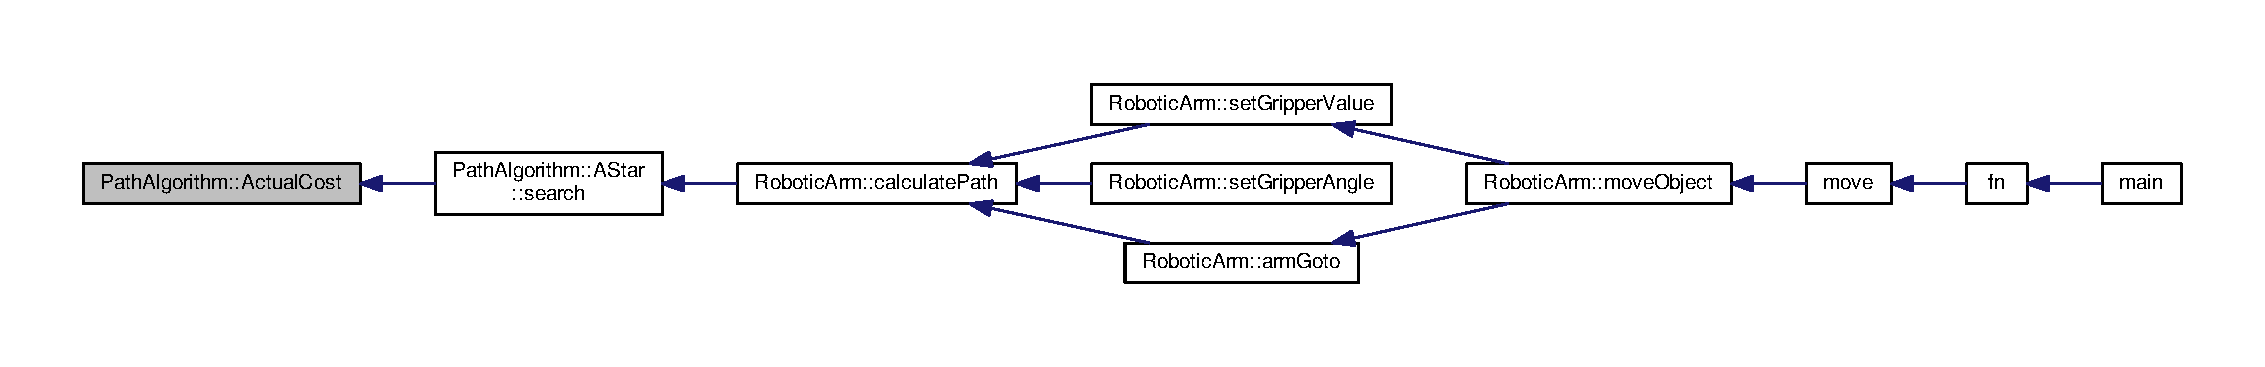
\includegraphics[width=350pt]{namespace_path_algorithm_a303daba8d3a083b341d1f4a799c3d5e4_icgraph}
\end{center}
\end{figure}


\index{Path\+Algorithm@{Path\+Algorithm}!Construct\+Path@{Construct\+Path}}
\index{Construct\+Path@{Construct\+Path}!Path\+Algorithm@{Path\+Algorithm}}
\subsubsection[{\texorpdfstring{Construct\+Path(\+Vertex\+Map \&a\+Predecessor\+Map, const Vertex \&a\+Current\+Node)}{ConstructPath(VertexMap &aPredecessorMap, const Vertex &aCurrentNode)}}]{\setlength{\rightskip}{0pt plus 5cm}{\bf Path} Path\+Algorithm\+::\+Construct\+Path (
\begin{DoxyParamCaption}
\item[{{\bf Vertex\+Map} \&}]{a\+Predecessor\+Map, }
\item[{const {\bf Vertex} \&}]{a\+Current\+Node}
\end{DoxyParamCaption}
)}\hypertarget{namespace_path_algorithm_a1b72e8125a5f9fa31d3130c816f1a03f}{}\label{namespace_path_algorithm_a1b72e8125a5f9fa31d3130c816f1a03f}


Definition at line 28 of file A\+Star.\+cpp.



Here is the caller graph for this function\+:\nopagebreak
\begin{figure}[H]
\begin{center}
\leavevmode
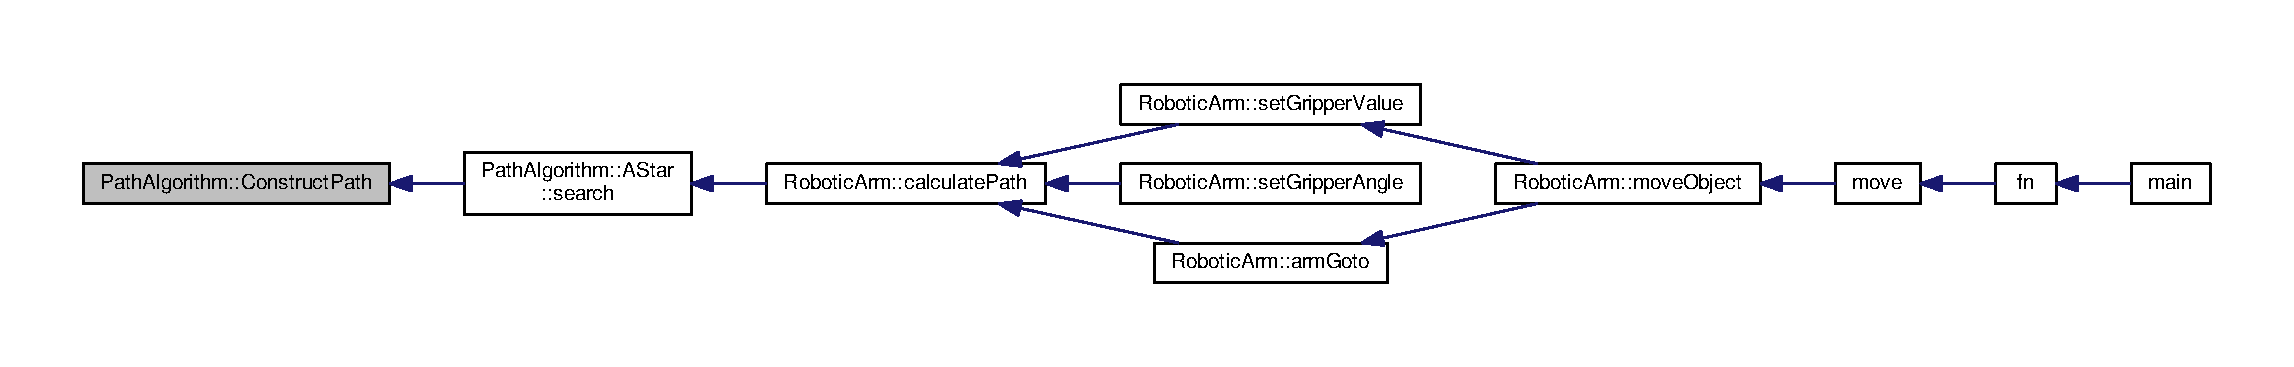
\includegraphics[width=350pt]{namespace_path_algorithm_a1b72e8125a5f9fa31d3130c816f1a03f_icgraph}
\end{center}
\end{figure}


\index{Path\+Algorithm@{Path\+Algorithm}!forward\+Kinematics@{forward\+Kinematics}}
\index{forward\+Kinematics@{forward\+Kinematics}!Path\+Algorithm@{Path\+Algorithm}}
\subsubsection[{\texorpdfstring{forward\+Kinematics(double x0, double y0, double a, double p1, double b, double p2)}{forwardKinematics(double x0, double y0, double a, double p1, double b, double p2)}}]{\setlength{\rightskip}{0pt plus 5cm}std\+::pair$<$double, double$>$ Path\+Algorithm\+::forward\+Kinematics (
\begin{DoxyParamCaption}
\item[{double}]{x0, }
\item[{double}]{y0, }
\item[{double}]{a, }
\item[{double}]{p1, }
\item[{double}]{b, }
\item[{double}]{p2}
\end{DoxyParamCaption}
)}\hypertarget{namespace_path_algorithm_aaa1cdbf02ad31d9d9f0161839a1af45d}{}\label{namespace_path_algorithm_aaa1cdbf02ad31d9d9f0161839a1af45d}
\index{Path\+Algorithm@{Path\+Algorithm}!Get\+Neighbour\+Connections@{Get\+Neighbour\+Connections}}
\index{Get\+Neighbour\+Connections@{Get\+Neighbour\+Connections}!Path\+Algorithm@{Path\+Algorithm}}
\subsubsection[{\texorpdfstring{Get\+Neighbour\+Connections(const Vertex \&a\+Vertex, int a\+Free\+Radius, Robotic\+Arm \&robot)}{GetNeighbourConnections(const Vertex &aVertex, int aFreeRadius, RoboticArm &robot)}}]{\setlength{\rightskip}{0pt plus 5cm}std\+::vector$<${\bf Edge}$>$ Path\+Algorithm\+::\+Get\+Neighbour\+Connections (
\begin{DoxyParamCaption}
\item[{const {\bf Vertex} \&}]{a\+Vertex, }
\item[{int}]{a\+Free\+Radius, }
\item[{{\bf Robotic\+Arm} \&}]{robot}
\end{DoxyParamCaption}
)}\hypertarget{namespace_path_algorithm_a8f0c4453fa932953ae67e31855f68197}{}\label{namespace_path_algorithm_a8f0c4453fa932953ae67e31855f68197}


Definition at line 84 of file A\+Star.\+cpp.



Here is the call graph for this function\+:\nopagebreak
\begin{figure}[H]
\begin{center}
\leavevmode
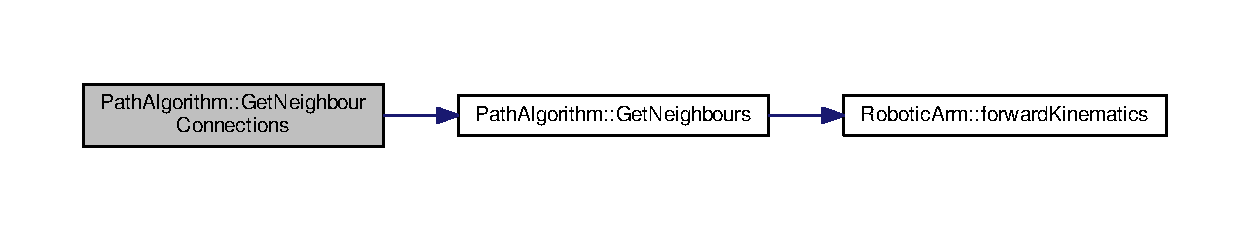
\includegraphics[width=350pt]{namespace_path_algorithm_a8f0c4453fa932953ae67e31855f68197_cgraph}
\end{center}
\end{figure}




Here is the caller graph for this function\+:\nopagebreak
\begin{figure}[H]
\begin{center}
\leavevmode
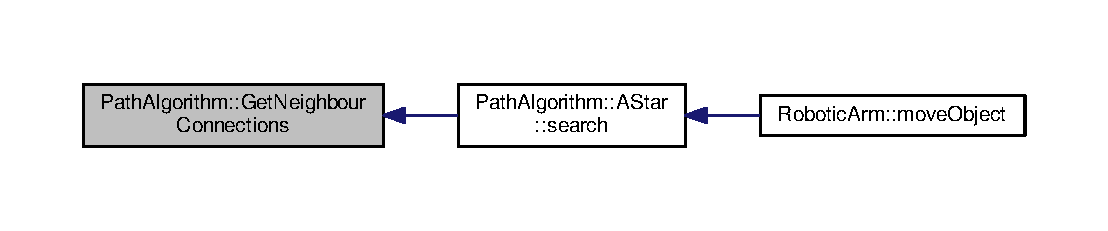
\includegraphics[width=350pt]{namespace_path_algorithm_a8f0c4453fa932953ae67e31855f68197_icgraph}
\end{center}
\end{figure}


\index{Path\+Algorithm@{Path\+Algorithm}!Get\+Neighbours@{Get\+Neighbours}}
\index{Get\+Neighbours@{Get\+Neighbours}!Path\+Algorithm@{Path\+Algorithm}}
\subsubsection[{\texorpdfstring{Get\+Neighbours(const Vertex \&a\+Vertex, int a\+Free\+Radius, Robotic\+Arm \&robot)}{GetNeighbours(const Vertex &aVertex, int aFreeRadius, RoboticArm &robot)}}]{\setlength{\rightskip}{0pt plus 5cm}std\+::vector$<${\bf Vertex}$>$ Path\+Algorithm\+::\+Get\+Neighbours (
\begin{DoxyParamCaption}
\item[{const {\bf Vertex} \&}]{a\+Vertex, }
\item[{int}]{a\+Free\+Radius, }
\item[{{\bf Robotic\+Arm} \&}]{robot}
\end{DoxyParamCaption}
)}\hypertarget{namespace_path_algorithm_ae4490c66af669f70064a693a8d7a889e}{}\label{namespace_path_algorithm_ae4490c66af669f70064a693a8d7a889e}


Definition at line 47 of file A\+Star.\+cpp.



Here is the call graph for this function\+:\nopagebreak
\begin{figure}[H]
\begin{center}
\leavevmode
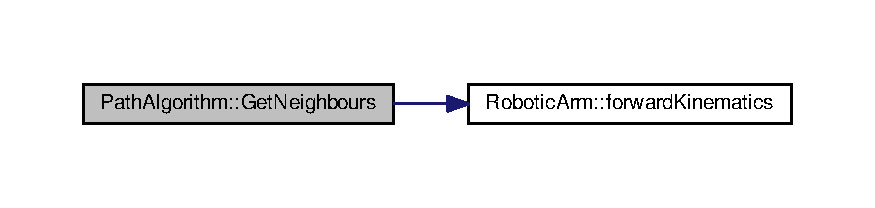
\includegraphics[width=350pt]{namespace_path_algorithm_ae4490c66af669f70064a693a8d7a889e_cgraph}
\end{center}
\end{figure}




Here is the caller graph for this function\+:\nopagebreak
\begin{figure}[H]
\begin{center}
\leavevmode
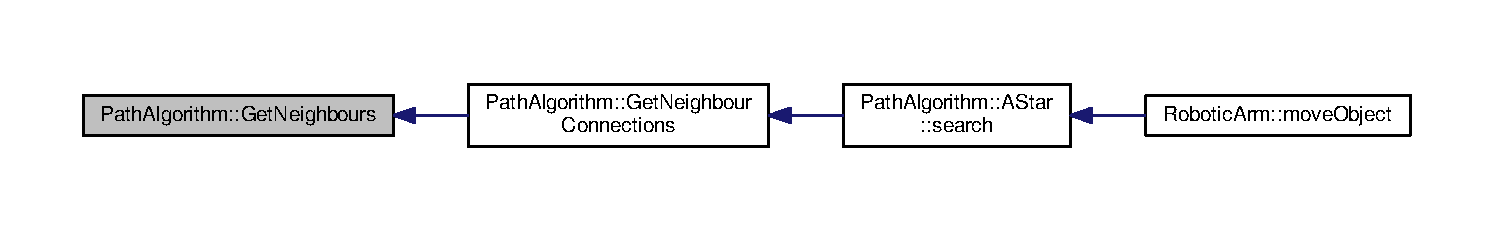
\includegraphics[width=350pt]{namespace_path_algorithm_ae4490c66af669f70064a693a8d7a889e_icgraph}
\end{center}
\end{figure}


\index{Path\+Algorithm@{Path\+Algorithm}!Heuristic\+Cost@{Heuristic\+Cost}}
\index{Heuristic\+Cost@{Heuristic\+Cost}!Path\+Algorithm@{Path\+Algorithm}}
\subsubsection[{\texorpdfstring{Heuristic\+Cost(const Vertex \&a\+Start, const Vertex \&a\+Goal)}{HeuristicCost(const Vertex &aStart, const Vertex &aGoal)}}]{\setlength{\rightskip}{0pt plus 5cm}double Path\+Algorithm\+::\+Heuristic\+Cost (
\begin{DoxyParamCaption}
\item[{const {\bf Vertex} \&}]{a\+Start, }
\item[{const {\bf Vertex} \&}]{a\+Goal}
\end{DoxyParamCaption}
)}\hypertarget{namespace_path_algorithm_a2e4474691c7ebd46c7238f2c53b0e543}{}\label{namespace_path_algorithm_a2e4474691c7ebd46c7238f2c53b0e543}


Definition at line 21 of file A\+Star.\+cpp.



Here is the caller graph for this function\+:\nopagebreak
\begin{figure}[H]
\begin{center}
\leavevmode
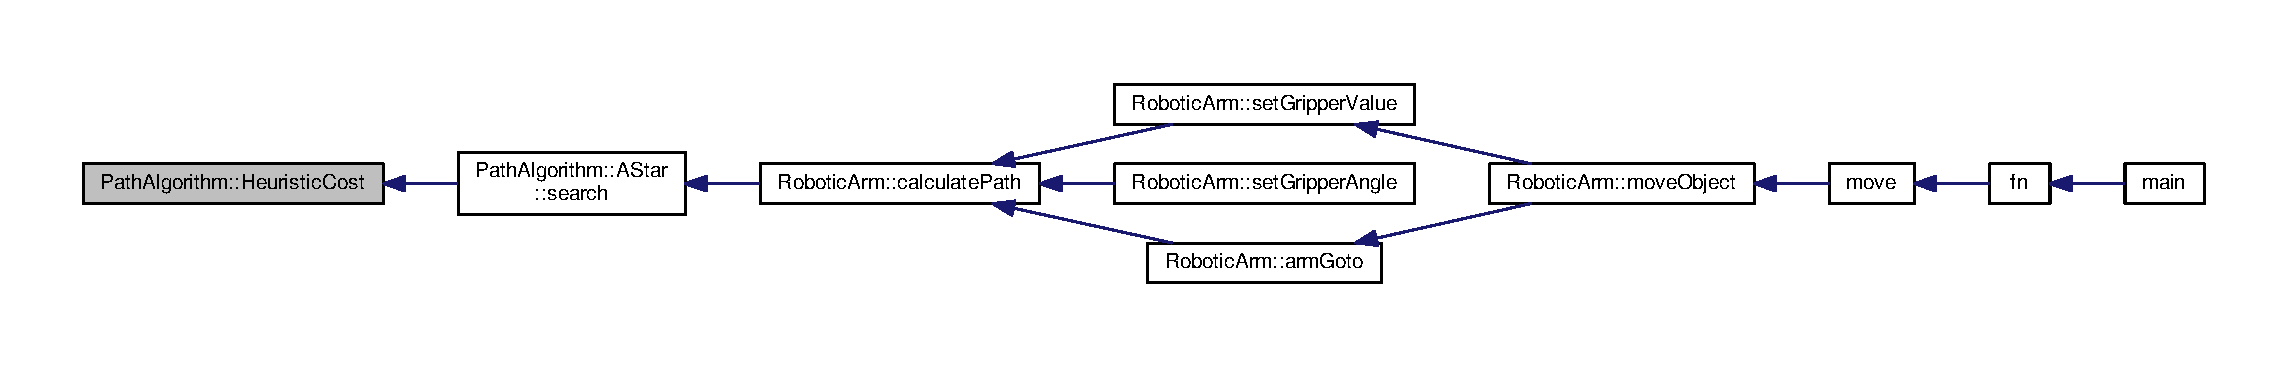
\includegraphics[width=350pt]{namespace_path_algorithm_a2e4474691c7ebd46c7238f2c53b0e543_icgraph}
\end{center}
\end{figure}


\index{Path\+Algorithm@{Path\+Algorithm}!operator$<$$<$@{operator$<$$<$}}
\index{operator$<$$<$@{operator$<$$<$}!Path\+Algorithm@{Path\+Algorithm}}
\subsubsection[{\texorpdfstring{operator$<$$<$(std\+::ostream \&os, const Vertex \&a\+Vertex)}{operator<<(std::ostream &os, const Vertex &aVertex)}}]{\setlength{\rightskip}{0pt plus 5cm}std\+::ostream\& Path\+Algorithm\+::operator$<$$<$ (
\begin{DoxyParamCaption}
\item[{std\+::ostream \&}]{os, }
\item[{const {\bf Vertex} \&}]{a\+Vertex}
\end{DoxyParamCaption}
)\hspace{0.3cm}{\ttfamily [inline]}}\hypertarget{namespace_path_algorithm_a7570fe9b9ed95b023311d0b9ef75b7ea}{}\label{namespace_path_algorithm_a7570fe9b9ed95b023311d0b9ef75b7ea}

\begin{DoxyParams}{Parameters}
{\em os} & \\
\hline
{\em a\+Vertex} & \\
\hline
\end{DoxyParams}
\begin{DoxyReturn}{Returns}

\end{DoxyReturn}


Definition at line 173 of file A\+Star.\+hpp.

\index{Path\+Algorithm@{Path\+Algorithm}!operator$<$$<$@{operator$<$$<$}}
\index{operator$<$$<$@{operator$<$$<$}!Path\+Algorithm@{Path\+Algorithm}}
\subsubsection[{\texorpdfstring{operator$<$$<$(std\+::ostream \&os, const Edge \&an\+Edge)}{operator<<(std::ostream &os, const Edge &anEdge)}}]{\setlength{\rightskip}{0pt plus 5cm}std\+::ostream\& Path\+Algorithm\+::operator$<$$<$ (
\begin{DoxyParamCaption}
\item[{std\+::ostream \&}]{os, }
\item[{const {\bf Edge} \&}]{an\+Edge}
\end{DoxyParamCaption}
)\hspace{0.3cm}{\ttfamily [inline]}}\hypertarget{namespace_path_algorithm_a4d00bd2dacc6db331429deab0d46cbf3}{}\label{namespace_path_algorithm_a4d00bd2dacc6db331429deab0d46cbf3}

\begin{DoxyParams}{Parameters}
{\em os} & \\
\hline
{\em an\+Edge} & \\
\hline
\end{DoxyParams}
\begin{DoxyReturn}{Returns}

\end{DoxyReturn}


Definition at line 183 of file A\+Star.\+hpp.


\hypertarget{namespacerobot_point}{}\section{robot\+Point Namespace Reference}
\label{namespacerobot_point}\index{robot\+Point@{robot\+Point}}
\subsection*{Classes}
\begin{DoxyCompactItemize}
\item 
struct \hyperlink{structrobot_point_1_1_point}{Point}
\end{DoxyCompactItemize}

\hypertarget{namespaceserial}{}\section{serial Namespace Reference}
\label{namespaceserial}\index{serial@{serial}}
\subsection*{Namespaces}
\begin{DoxyCompactItemize}
\item 
 \hyperlink{namespaceserial_1_1_serial}{Serial}
\end{DoxyCompactItemize}

\hypertarget{namespaceserial_1_1_serial}{}\section{serial\+:\+:Serial Namespace Reference}
\label{namespaceserial_1_1_serial}\index{serial\+::\+Serial@{serial\+::\+Serial}}
\subsection*{Classes}
\begin{DoxyCompactItemize}
\item 
class \hyperlink{class_serial_1_1_scoped_read_lock}{Scoped\+Read\+Lock}
\item 
class \hyperlink{class_serial_1_1_scoped_write_lock}{Scoped\+Write\+Lock}
\end{DoxyCompactItemize}

\hypertarget{namespace_widgets}{}\section{Widgets Namespace Reference}
\label{namespace_widgets}\index{Widgets@{Widgets}}
\subsection*{Classes}
\begin{DoxyCompactItemize}
\item 
struct \hyperlink{struct_widgets_1_1_size}{Size}
\end{DoxyCompactItemize}

\chapter{Class Documentation}
\hypertarget{class_path_algorithm_1_1_a_star}{}\section{Path\+Algorithm\+:\+:A\+Star Class Reference}
\label{class_path_algorithm_1_1_a_star}\index{Path\+Algorithm\+::\+A\+Star@{Path\+Algorithm\+::\+A\+Star}}


{\ttfamily \#include $<$A\+Star.\+hpp$>$}

\subsection*{Public Member Functions}
\begin{DoxyCompactItemize}
\item 
\hyperlink{namespace_path_algorithm_a7f2958a43117506f3cb6dc9409a22c0d}{Path} \hyperlink{class_path_algorithm_1_1_a_star_aee41b31ec44b02f6dc94889d228a3582}{search} (\hyperlink{struct_path_algorithm_1_1_vertex}{Vertex} a\+Start, const \hyperlink{struct_path_algorithm_1_1_vertex}{Vertex} \&a\+Goal, const \hyperlink{struct_widgets_1_1_size}{Size} \&a\+Robot\+Size, \hyperlink{class_robotic_arm}{Robotic\+Arm} \&robot)
\item 
void \hyperlink{class_path_algorithm_1_1_a_star_a63f88f24acf7bf34cd060051134c9190}{add\+To\+Open\+Set} (const \hyperlink{struct_path_algorithm_1_1_vertex}{Vertex} \&a\+Vertex)
\item 
void \hyperlink{class_path_algorithm_1_1_a_star_afcc23a676145d6e280d1c3430af5380a}{remove\+From\+Open\+Set} (const \hyperlink{struct_path_algorithm_1_1_vertex}{Vertex} \&a\+Vertex)
\item 
void \hyperlink{class_path_algorithm_1_1_a_star_aba29c2585fbf49880cf5e8b9bf6d3eb5}{remove\+From\+Open\+Set} (Open\+Set\+::iterator \&i)
\item 
Open\+Set\+::iterator \hyperlink{class_path_algorithm_1_1_a_star_ae78bfebdee31135fdfb2f302347f962f}{find\+In\+Open\+Set} (const \hyperlink{struct_path_algorithm_1_1_vertex}{Vertex} \&a\+Vertex)
\item 
bool \hyperlink{class_path_algorithm_1_1_a_star_a657aaaf577ca25e68e6a5af57214e7d4}{find\+Remove\+In\+Open\+Set} (const \hyperlink{struct_path_algorithm_1_1_vertex}{Vertex} \&a\+Vertex)
\item 
void \hyperlink{class_path_algorithm_1_1_a_star_a5bb18edbbd54833aac9eddfe63ba652d}{remove\+First\+From\+Open\+Set} ()
\item 
void \hyperlink{class_path_algorithm_1_1_a_star_a53139e4b3cd3971a2bf85a430e83378f}{add\+To\+Closed\+Set} (const \hyperlink{struct_path_algorithm_1_1_vertex}{Vertex} \&a\+Vertex)
\item 
void \hyperlink{class_path_algorithm_1_1_a_star_a1b6971a9c5878e859cbdb3270dda93b4}{remove\+From\+Closed\+Set} (const \hyperlink{struct_path_algorithm_1_1_vertex}{Vertex} \&a\+Vertex)
\item 
void \hyperlink{class_path_algorithm_1_1_a_star_a799953993c1255f0ce559f7233d3c926}{remove\+From\+Closed\+Set} (Closed\+Set\+::iterator \&i)
\item 
Closed\+Set\+::iterator \hyperlink{class_path_algorithm_1_1_a_star_a73d9639e838fd55bb392d01238fc967a}{find\+In\+Closed\+Set} (const \hyperlink{struct_path_algorithm_1_1_vertex}{Vertex} \&a\+Vertex)
\item 
bool \hyperlink{class_path_algorithm_1_1_a_star_a843db81c9950c0184ee31627313f5793}{find\+Remove\+Closed\+Set} (const \hyperlink{struct_path_algorithm_1_1_vertex}{Vertex} \&a\+Vertex)
\item 
\hyperlink{namespace_path_algorithm_ac027c23e4b4c237b6eb96fc63d79266f}{Closed\+Set} \hyperlink{class_path_algorithm_1_1_a_star_a94fcc29f04e6398edbd58effbf59b49a}{get\+Closed\+Set} () const 
\item 
\hyperlink{namespace_path_algorithm_a999fc5baea7d1f71e42570630a297029}{Open\+Set} \hyperlink{class_path_algorithm_1_1_a_star_ae419f2d019378d9b4435d862b70da72f}{get\+Open\+Set} () const 
\item 
\hyperlink{namespace_path_algorithm_ac8a52a9740a0bfa959810bd92e08d962}{Vertex\+Map} \hyperlink{class_path_algorithm_1_1_a_star_ac4ce233712c0f7aac44d029e61888581}{get\+Predecessor\+Map} () const 
\end{DoxyCompactItemize}
\subsection*{Protected Member Functions}
\begin{DoxyCompactItemize}
\item 
\hyperlink{namespace_path_algorithm_ac027c23e4b4c237b6eb96fc63d79266f}{Closed\+Set} \& \hyperlink{class_path_algorithm_1_1_a_star_a4cb2a6c928a01fcac02533500bd8ace5}{get\+CS} ()
\item 
const \hyperlink{namespace_path_algorithm_ac027c23e4b4c237b6eb96fc63d79266f}{Closed\+Set} \& \hyperlink{class_path_algorithm_1_1_a_star_a420e1ac8824a265dc2272c7e50899322}{get\+CS} () const 
\item 
\hyperlink{namespace_path_algorithm_a999fc5baea7d1f71e42570630a297029}{Open\+Set} \& \hyperlink{class_path_algorithm_1_1_a_star_a48e23107ffca02392bdf2439775baecf}{get\+OS} ()
\item 
const \hyperlink{namespace_path_algorithm_a999fc5baea7d1f71e42570630a297029}{Open\+Set} \& \hyperlink{class_path_algorithm_1_1_a_star_af5ea4271f9318edaa68d8030e35d0cf1}{get\+OS} () const 
\item 
\hyperlink{namespace_path_algorithm_ac8a52a9740a0bfa959810bd92e08d962}{Vertex\+Map} \& \hyperlink{class_path_algorithm_1_1_a_star_a4bb6718fd07f503ff836c5cdccd74236}{get\+PM} ()
\item 
const \hyperlink{namespace_path_algorithm_ac8a52a9740a0bfa959810bd92e08d962}{Vertex\+Map} \& \hyperlink{class_path_algorithm_1_1_a_star_a021ff514f018ce9ec7db705578a210d4}{get\+PM} () const 
\end{DoxyCompactItemize}


\subsection{Detailed Description}


Definition at line 197 of file A\+Star.\+hpp.



\subsection{Member Function Documentation}
\index{Path\+Algorithm\+::\+A\+Star@{Path\+Algorithm\+::\+A\+Star}!add\+To\+Closed\+Set@{add\+To\+Closed\+Set}}
\index{add\+To\+Closed\+Set@{add\+To\+Closed\+Set}!Path\+Algorithm\+::\+A\+Star@{Path\+Algorithm\+::\+A\+Star}}
\subsubsection[{\texorpdfstring{add\+To\+Closed\+Set(const Vertex \&a\+Vertex)}{addToClosedSet(const Vertex &aVertex)}}]{\setlength{\rightskip}{0pt plus 5cm}void Path\+Algorithm\+::\+A\+Star\+::add\+To\+Closed\+Set (
\begin{DoxyParamCaption}
\item[{const {\bf Vertex} \&}]{a\+Vertex}
\end{DoxyParamCaption}
)}\hypertarget{class_path_algorithm_1_1_a_star_a53139e4b3cd3971a2bf85a430e83378f}{}\label{class_path_algorithm_1_1_a_star_a53139e4b3cd3971a2bf85a430e83378f}


Definition at line 316 of file A\+Star.\+cpp.



Here is the caller graph for this function\+:\nopagebreak
\begin{figure}[H]
\begin{center}
\leavevmode
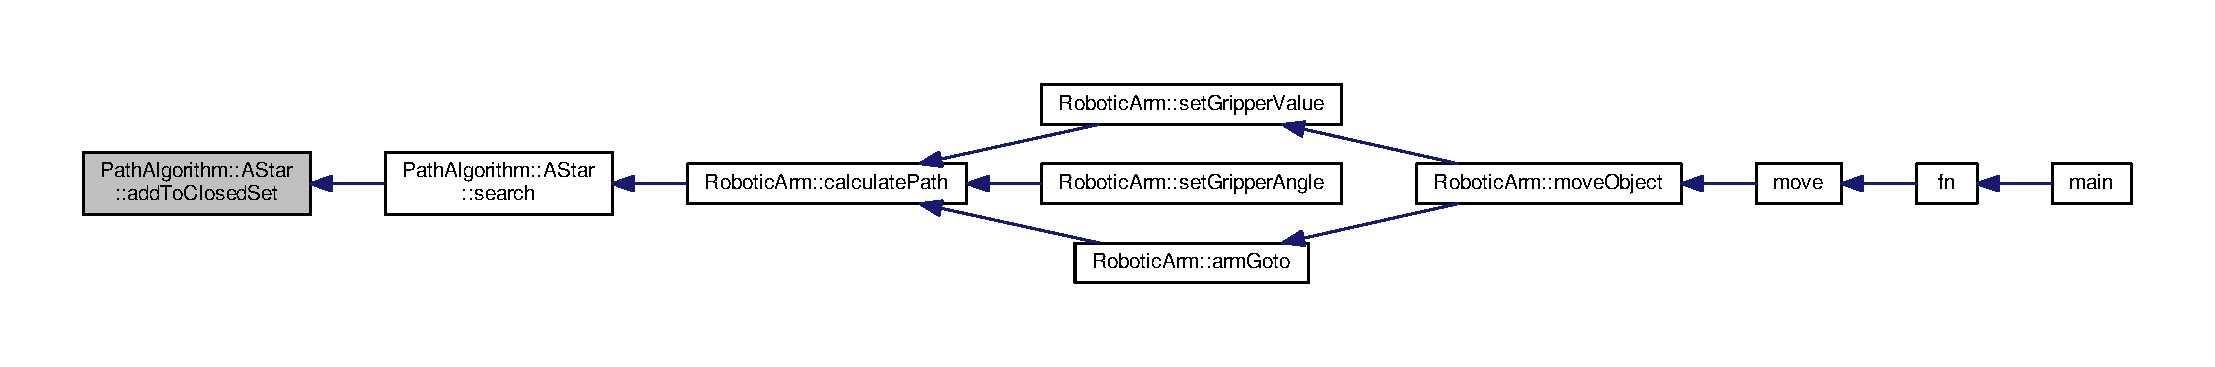
\includegraphics[width=350pt]{class_path_algorithm_1_1_a_star_a53139e4b3cd3971a2bf85a430e83378f_icgraph}
\end{center}
\end{figure}


\index{Path\+Algorithm\+::\+A\+Star@{Path\+Algorithm\+::\+A\+Star}!add\+To\+Open\+Set@{add\+To\+Open\+Set}}
\index{add\+To\+Open\+Set@{add\+To\+Open\+Set}!Path\+Algorithm\+::\+A\+Star@{Path\+Algorithm\+::\+A\+Star}}
\subsubsection[{\texorpdfstring{add\+To\+Open\+Set(const Vertex \&a\+Vertex)}{addToOpenSet(const Vertex &aVertex)}}]{\setlength{\rightskip}{0pt plus 5cm}void Path\+Algorithm\+::\+A\+Star\+::add\+To\+Open\+Set (
\begin{DoxyParamCaption}
\item[{const {\bf Vertex} \&}]{a\+Vertex}
\end{DoxyParamCaption}
)}\hypertarget{class_path_algorithm_1_1_a_star_a63f88f24acf7bf34cd060051134c9190}{}\label{class_path_algorithm_1_1_a_star_a63f88f24acf7bf34cd060051134c9190}


Definition at line 255 of file A\+Star.\+cpp.



Here is the caller graph for this function\+:\nopagebreak
\begin{figure}[H]
\begin{center}
\leavevmode
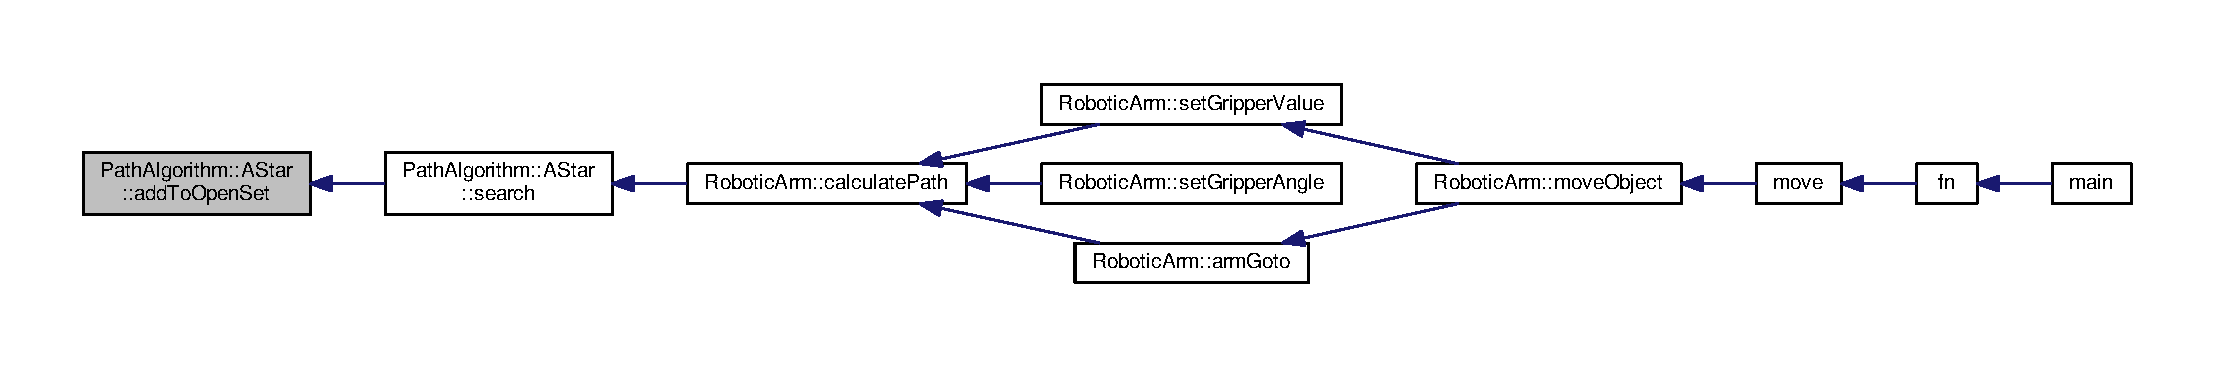
\includegraphics[width=350pt]{class_path_algorithm_1_1_a_star_a63f88f24acf7bf34cd060051134c9190_icgraph}
\end{center}
\end{figure}


\index{Path\+Algorithm\+::\+A\+Star@{Path\+Algorithm\+::\+A\+Star}!find\+In\+Closed\+Set@{find\+In\+Closed\+Set}}
\index{find\+In\+Closed\+Set@{find\+In\+Closed\+Set}!Path\+Algorithm\+::\+A\+Star@{Path\+Algorithm\+::\+A\+Star}}
\subsubsection[{\texorpdfstring{find\+In\+Closed\+Set(const Vertex \&a\+Vertex)}{findInClosedSet(const Vertex &aVertex)}}]{\setlength{\rightskip}{0pt plus 5cm}Closed\+Set\+::iterator Path\+Algorithm\+::\+A\+Star\+::find\+In\+Closed\+Set (
\begin{DoxyParamCaption}
\item[{const {\bf Vertex} \&}]{a\+Vertex}
\end{DoxyParamCaption}
)}\hypertarget{class_path_algorithm_1_1_a_star_a73d9639e838fd55bb392d01238fc967a}{}\label{class_path_algorithm_1_1_a_star_a73d9639e838fd55bb392d01238fc967a}


Definition at line 343 of file A\+Star.\+cpp.



Here is the caller graph for this function\+:\nopagebreak
\begin{figure}[H]
\begin{center}
\leavevmode
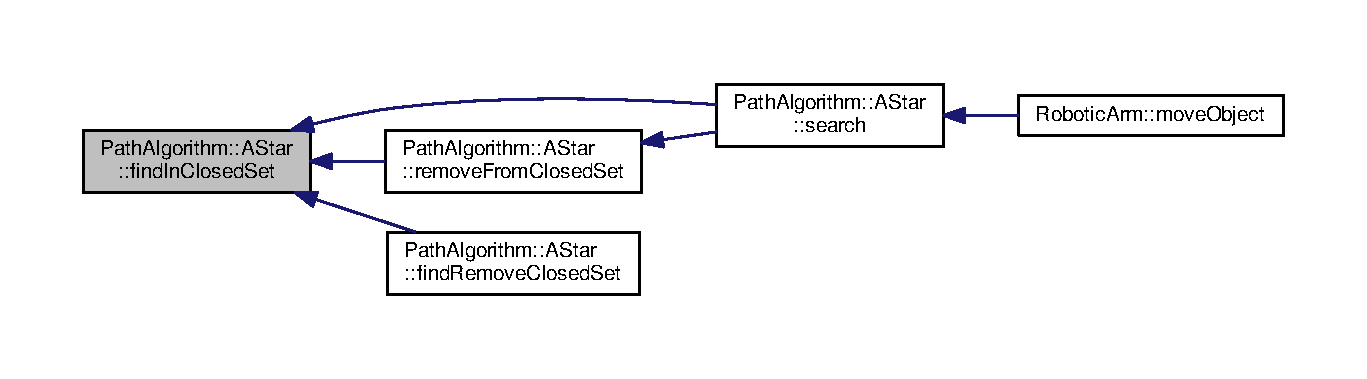
\includegraphics[width=350pt]{class_path_algorithm_1_1_a_star_a73d9639e838fd55bb392d01238fc967a_icgraph}
\end{center}
\end{figure}


\index{Path\+Algorithm\+::\+A\+Star@{Path\+Algorithm\+::\+A\+Star}!find\+In\+Open\+Set@{find\+In\+Open\+Set}}
\index{find\+In\+Open\+Set@{find\+In\+Open\+Set}!Path\+Algorithm\+::\+A\+Star@{Path\+Algorithm\+::\+A\+Star}}
\subsubsection[{\texorpdfstring{find\+In\+Open\+Set(const Vertex \&a\+Vertex)}{findInOpenSet(const Vertex &aVertex)}}]{\setlength{\rightskip}{0pt plus 5cm}Open\+Set\+::iterator Path\+Algorithm\+::\+A\+Star\+::find\+In\+Open\+Set (
\begin{DoxyParamCaption}
\item[{const {\bf Vertex} \&}]{a\+Vertex}
\end{DoxyParamCaption}
)}\hypertarget{class_path_algorithm_1_1_a_star_ae78bfebdee31135fdfb2f302347f962f}{}\label{class_path_algorithm_1_1_a_star_ae78bfebdee31135fdfb2f302347f962f}


Definition at line 282 of file A\+Star.\+cpp.



Here is the call graph for this function\+:\nopagebreak
\begin{figure}[H]
\begin{center}
\leavevmode
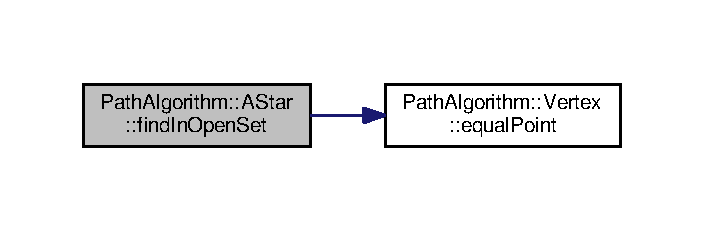
\includegraphics[width=338pt]{class_path_algorithm_1_1_a_star_ae78bfebdee31135fdfb2f302347f962f_cgraph}
\end{center}
\end{figure}




Here is the caller graph for this function\+:\nopagebreak
\begin{figure}[H]
\begin{center}
\leavevmode
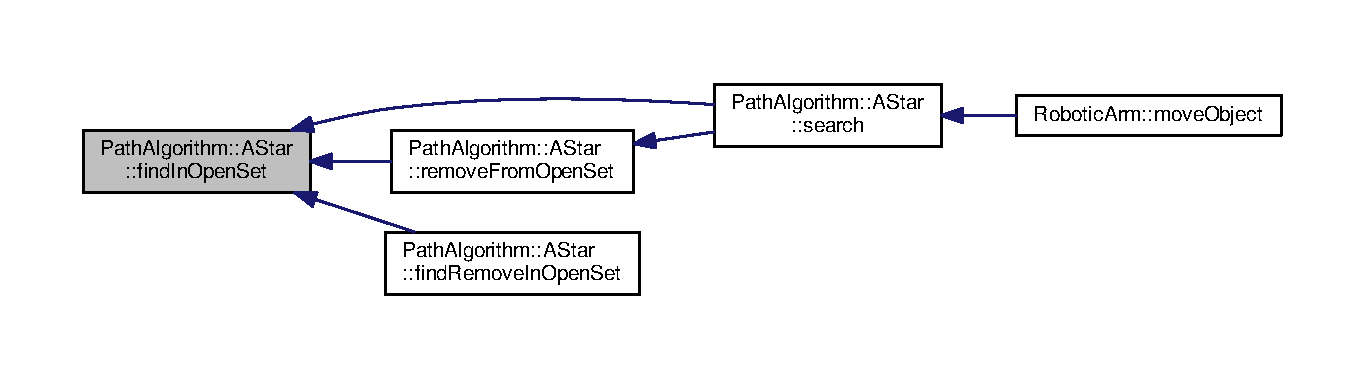
\includegraphics[width=350pt]{class_path_algorithm_1_1_a_star_ae78bfebdee31135fdfb2f302347f962f_icgraph}
\end{center}
\end{figure}


\index{Path\+Algorithm\+::\+A\+Star@{Path\+Algorithm\+::\+A\+Star}!find\+Remove\+Closed\+Set@{find\+Remove\+Closed\+Set}}
\index{find\+Remove\+Closed\+Set@{find\+Remove\+Closed\+Set}!Path\+Algorithm\+::\+A\+Star@{Path\+Algorithm\+::\+A\+Star}}
\subsubsection[{\texorpdfstring{find\+Remove\+Closed\+Set(const Vertex \&a\+Vertex)}{findRemoveClosedSet(const Vertex &aVertex)}}]{\setlength{\rightskip}{0pt plus 5cm}bool Path\+Algorithm\+::\+A\+Star\+::find\+Remove\+Closed\+Set (
\begin{DoxyParamCaption}
\item[{const {\bf Vertex} \&}]{a\+Vertex}
\end{DoxyParamCaption}
)}\hypertarget{class_path_algorithm_1_1_a_star_a843db81c9950c0184ee31627313f5793}{}\label{class_path_algorithm_1_1_a_star_a843db81c9950c0184ee31627313f5793}


Definition at line 361 of file A\+Star.\+cpp.



Here is the call graph for this function\+:\nopagebreak
\begin{figure}[H]
\begin{center}
\leavevmode
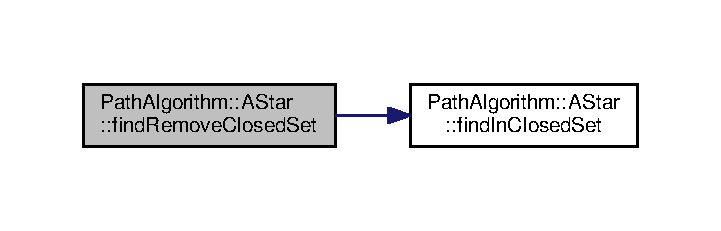
\includegraphics[width=346pt]{class_path_algorithm_1_1_a_star_a843db81c9950c0184ee31627313f5793_cgraph}
\end{center}
\end{figure}


\index{Path\+Algorithm\+::\+A\+Star@{Path\+Algorithm\+::\+A\+Star}!find\+Remove\+In\+Open\+Set@{find\+Remove\+In\+Open\+Set}}
\index{find\+Remove\+In\+Open\+Set@{find\+Remove\+In\+Open\+Set}!Path\+Algorithm\+::\+A\+Star@{Path\+Algorithm\+::\+A\+Star}}
\subsubsection[{\texorpdfstring{find\+Remove\+In\+Open\+Set(const Vertex \&a\+Vertex)}{findRemoveInOpenSet(const Vertex &aVertex)}}]{\setlength{\rightskip}{0pt plus 5cm}bool Path\+Algorithm\+::\+A\+Star\+::find\+Remove\+In\+Open\+Set (
\begin{DoxyParamCaption}
\item[{const {\bf Vertex} \&}]{a\+Vertex}
\end{DoxyParamCaption}
)}\hypertarget{class_path_algorithm_1_1_a_star_a657aaaf577ca25e68e6a5af57214e7d4}{}\label{class_path_algorithm_1_1_a_star_a657aaaf577ca25e68e6a5af57214e7d4}


Definition at line 293 of file A\+Star.\+cpp.



Here is the call graph for this function\+:\nopagebreak
\begin{figure}[H]
\begin{center}
\leavevmode
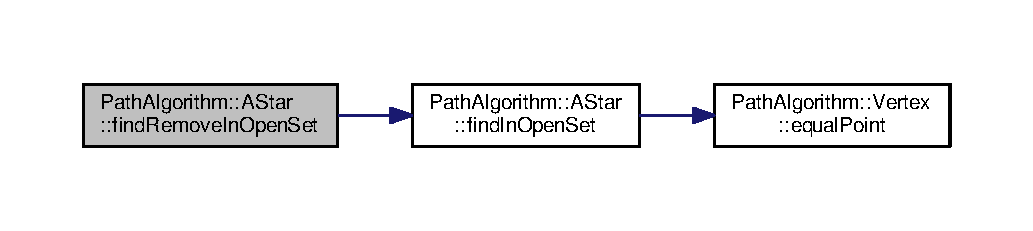
\includegraphics[width=350pt]{class_path_algorithm_1_1_a_star_a657aaaf577ca25e68e6a5af57214e7d4_cgraph}
\end{center}
\end{figure}


\index{Path\+Algorithm\+::\+A\+Star@{Path\+Algorithm\+::\+A\+Star}!get\+Closed\+Set@{get\+Closed\+Set}}
\index{get\+Closed\+Set@{get\+Closed\+Set}!Path\+Algorithm\+::\+A\+Star@{Path\+Algorithm\+::\+A\+Star}}
\subsubsection[{\texorpdfstring{get\+Closed\+Set() const }{getClosedSet() const }}]{\setlength{\rightskip}{0pt plus 5cm}{\bf Closed\+Set} Path\+Algorithm\+::\+A\+Star\+::get\+Closed\+Set (
\begin{DoxyParamCaption}
{}
\end{DoxyParamCaption}
) const}\hypertarget{class_path_algorithm_1_1_a_star_a94fcc29f04e6398edbd58effbf59b49a}{}\label{class_path_algorithm_1_1_a_star_a94fcc29f04e6398edbd58effbf59b49a}


Definition at line 352 of file A\+Star.\+cpp.



Here is the call graph for this function\+:\nopagebreak
\begin{figure}[H]
\begin{center}
\leavevmode
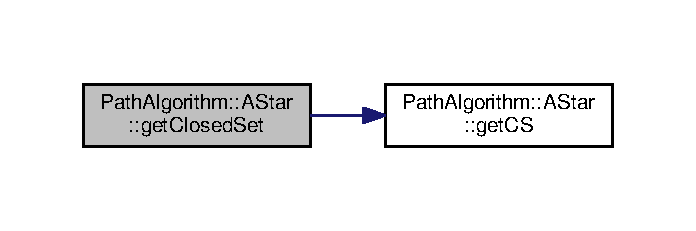
\includegraphics[width=334pt]{class_path_algorithm_1_1_a_star_a94fcc29f04e6398edbd58effbf59b49a_cgraph}
\end{center}
\end{figure}


\index{Path\+Algorithm\+::\+A\+Star@{Path\+Algorithm\+::\+A\+Star}!get\+CS@{get\+CS}}
\index{get\+CS@{get\+CS}!Path\+Algorithm\+::\+A\+Star@{Path\+Algorithm\+::\+A\+Star}}
\subsubsection[{\texorpdfstring{get\+C\+S()}{getCS()}}]{\setlength{\rightskip}{0pt plus 5cm}{\bf Closed\+Set} \& Path\+Algorithm\+::\+A\+Star\+::get\+CS (
\begin{DoxyParamCaption}
{}
\end{DoxyParamCaption}
)\hspace{0.3cm}{\ttfamily [protected]}}\hypertarget{class_path_algorithm_1_1_a_star_a4cb2a6c928a01fcac02533500bd8ace5}{}\label{class_path_algorithm_1_1_a_star_a4cb2a6c928a01fcac02533500bd8ace5}


Definition at line 394 of file A\+Star.\+cpp.



Here is the caller graph for this function\+:\nopagebreak
\begin{figure}[H]
\begin{center}
\leavevmode
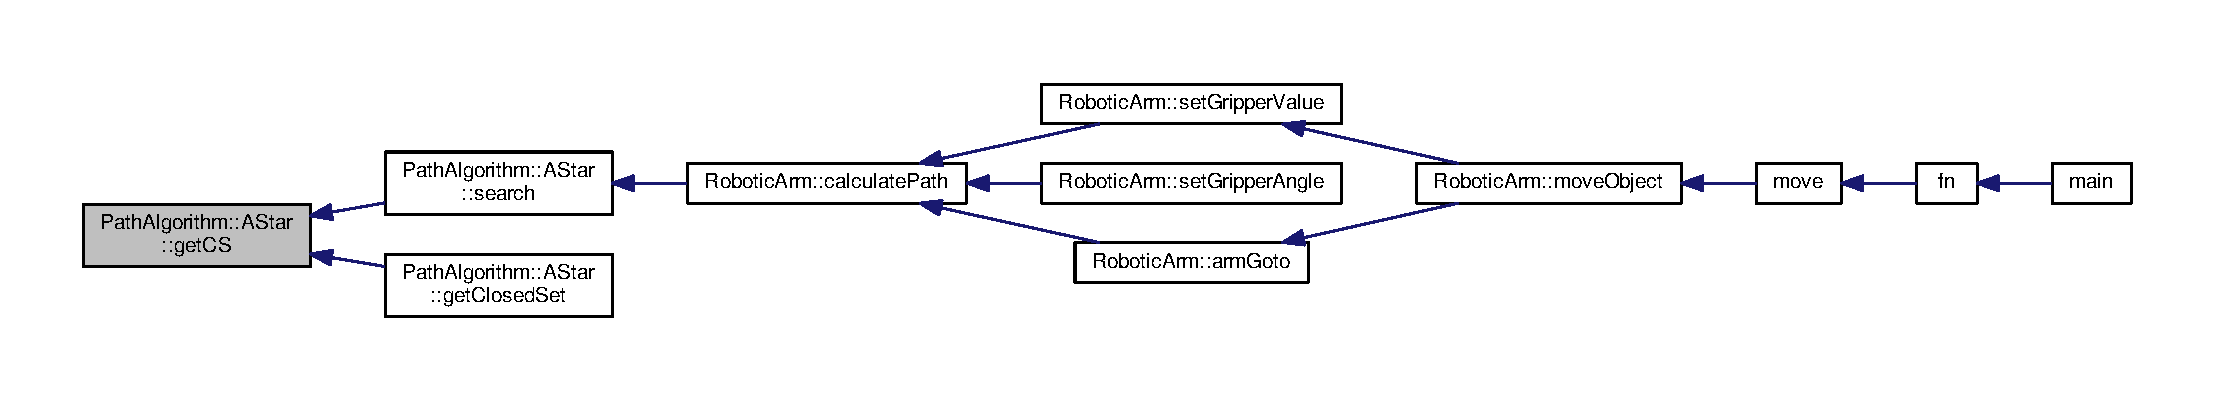
\includegraphics[width=350pt]{class_path_algorithm_1_1_a_star_a4cb2a6c928a01fcac02533500bd8ace5_icgraph}
\end{center}
\end{figure}


\index{Path\+Algorithm\+::\+A\+Star@{Path\+Algorithm\+::\+A\+Star}!get\+CS@{get\+CS}}
\index{get\+CS@{get\+CS}!Path\+Algorithm\+::\+A\+Star@{Path\+Algorithm\+::\+A\+Star}}
\subsubsection[{\texorpdfstring{get\+C\+S() const }{getCS() const }}]{\setlength{\rightskip}{0pt plus 5cm}const {\bf Closed\+Set} \& Path\+Algorithm\+::\+A\+Star\+::get\+CS (
\begin{DoxyParamCaption}
{}
\end{DoxyParamCaption}
) const\hspace{0.3cm}{\ttfamily [protected]}}\hypertarget{class_path_algorithm_1_1_a_star_a420e1ac8824a265dc2272c7e50899322}{}\label{class_path_algorithm_1_1_a_star_a420e1ac8824a265dc2272c7e50899322}


Definition at line 402 of file A\+Star.\+cpp.

\index{Path\+Algorithm\+::\+A\+Star@{Path\+Algorithm\+::\+A\+Star}!get\+Open\+Set@{get\+Open\+Set}}
\index{get\+Open\+Set@{get\+Open\+Set}!Path\+Algorithm\+::\+A\+Star@{Path\+Algorithm\+::\+A\+Star}}
\subsubsection[{\texorpdfstring{get\+Open\+Set() const }{getOpenSet() const }}]{\setlength{\rightskip}{0pt plus 5cm}{\bf Open\+Set} Path\+Algorithm\+::\+A\+Star\+::get\+Open\+Set (
\begin{DoxyParamCaption}
{}
\end{DoxyParamCaption}
) const}\hypertarget{class_path_algorithm_1_1_a_star_ae419f2d019378d9b4435d862b70da72f}{}\label{class_path_algorithm_1_1_a_star_ae419f2d019378d9b4435d862b70da72f}


Definition at line 375 of file A\+Star.\+cpp.



Here is the call graph for this function\+:\nopagebreak
\begin{figure}[H]
\begin{center}
\leavevmode
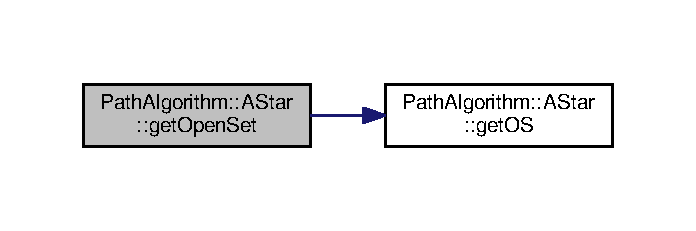
\includegraphics[width=334pt]{class_path_algorithm_1_1_a_star_ae419f2d019378d9b4435d862b70da72f_cgraph}
\end{center}
\end{figure}


\index{Path\+Algorithm\+::\+A\+Star@{Path\+Algorithm\+::\+A\+Star}!get\+OS@{get\+OS}}
\index{get\+OS@{get\+OS}!Path\+Algorithm\+::\+A\+Star@{Path\+Algorithm\+::\+A\+Star}}
\subsubsection[{\texorpdfstring{get\+O\+S()}{getOS()}}]{\setlength{\rightskip}{0pt plus 5cm}{\bf Open\+Set} \& Path\+Algorithm\+::\+A\+Star\+::get\+OS (
\begin{DoxyParamCaption}
{}
\end{DoxyParamCaption}
)\hspace{0.3cm}{\ttfamily [protected]}}\hypertarget{class_path_algorithm_1_1_a_star_a48e23107ffca02392bdf2439775baecf}{}\label{class_path_algorithm_1_1_a_star_a48e23107ffca02392bdf2439775baecf}


Definition at line 410 of file A\+Star.\+cpp.



Here is the caller graph for this function\+:\nopagebreak
\begin{figure}[H]
\begin{center}
\leavevmode
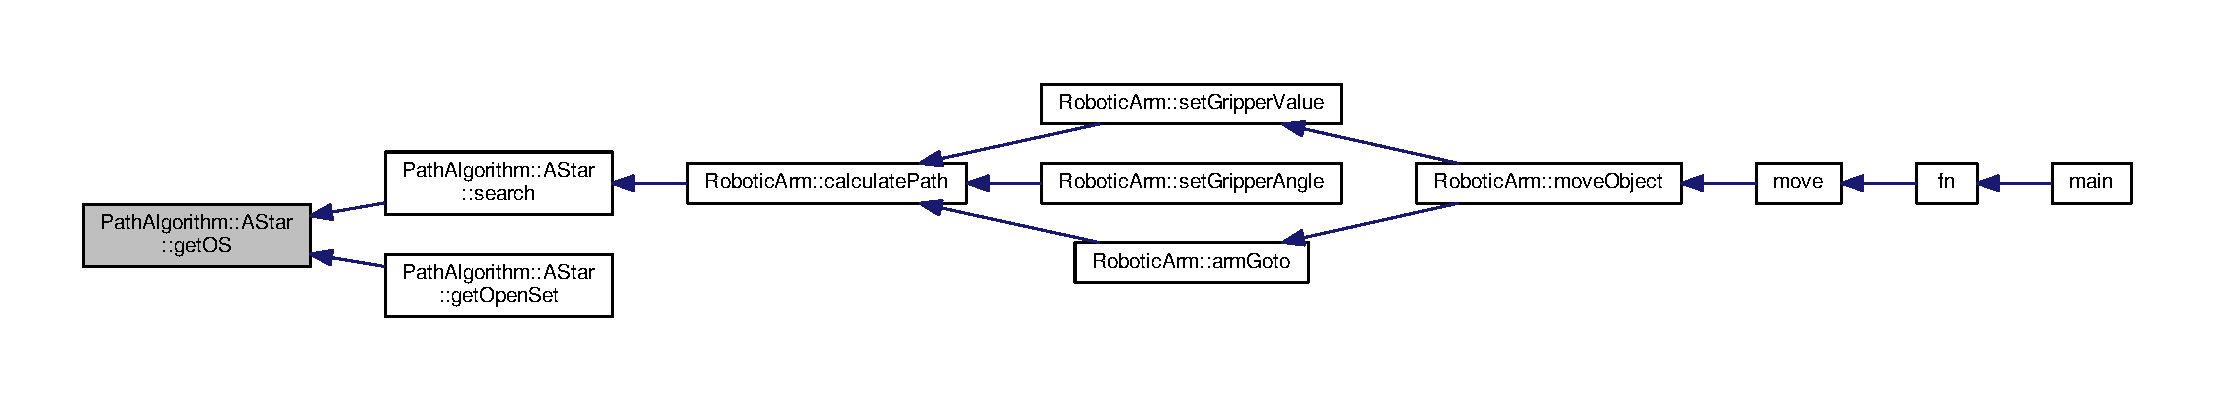
\includegraphics[width=350pt]{class_path_algorithm_1_1_a_star_a48e23107ffca02392bdf2439775baecf_icgraph}
\end{center}
\end{figure}


\index{Path\+Algorithm\+::\+A\+Star@{Path\+Algorithm\+::\+A\+Star}!get\+OS@{get\+OS}}
\index{get\+OS@{get\+OS}!Path\+Algorithm\+::\+A\+Star@{Path\+Algorithm\+::\+A\+Star}}
\subsubsection[{\texorpdfstring{get\+O\+S() const }{getOS() const }}]{\setlength{\rightskip}{0pt plus 5cm}const {\bf Open\+Set} \& Path\+Algorithm\+::\+A\+Star\+::get\+OS (
\begin{DoxyParamCaption}
{}
\end{DoxyParamCaption}
) const\hspace{0.3cm}{\ttfamily [protected]}}\hypertarget{class_path_algorithm_1_1_a_star_af5ea4271f9318edaa68d8030e35d0cf1}{}\label{class_path_algorithm_1_1_a_star_af5ea4271f9318edaa68d8030e35d0cf1}


Definition at line 418 of file A\+Star.\+cpp.

\index{Path\+Algorithm\+::\+A\+Star@{Path\+Algorithm\+::\+A\+Star}!get\+PM@{get\+PM}}
\index{get\+PM@{get\+PM}!Path\+Algorithm\+::\+A\+Star@{Path\+Algorithm\+::\+A\+Star}}
\subsubsection[{\texorpdfstring{get\+P\+M()}{getPM()}}]{\setlength{\rightskip}{0pt plus 5cm}{\bf Vertex\+Map} \& Path\+Algorithm\+::\+A\+Star\+::get\+PM (
\begin{DoxyParamCaption}
{}
\end{DoxyParamCaption}
)\hspace{0.3cm}{\ttfamily [protected]}}\hypertarget{class_path_algorithm_1_1_a_star_a4bb6718fd07f503ff836c5cdccd74236}{}\label{class_path_algorithm_1_1_a_star_a4bb6718fd07f503ff836c5cdccd74236}


Definition at line 426 of file A\+Star.\+cpp.



Here is the caller graph for this function\+:\nopagebreak
\begin{figure}[H]
\begin{center}
\leavevmode
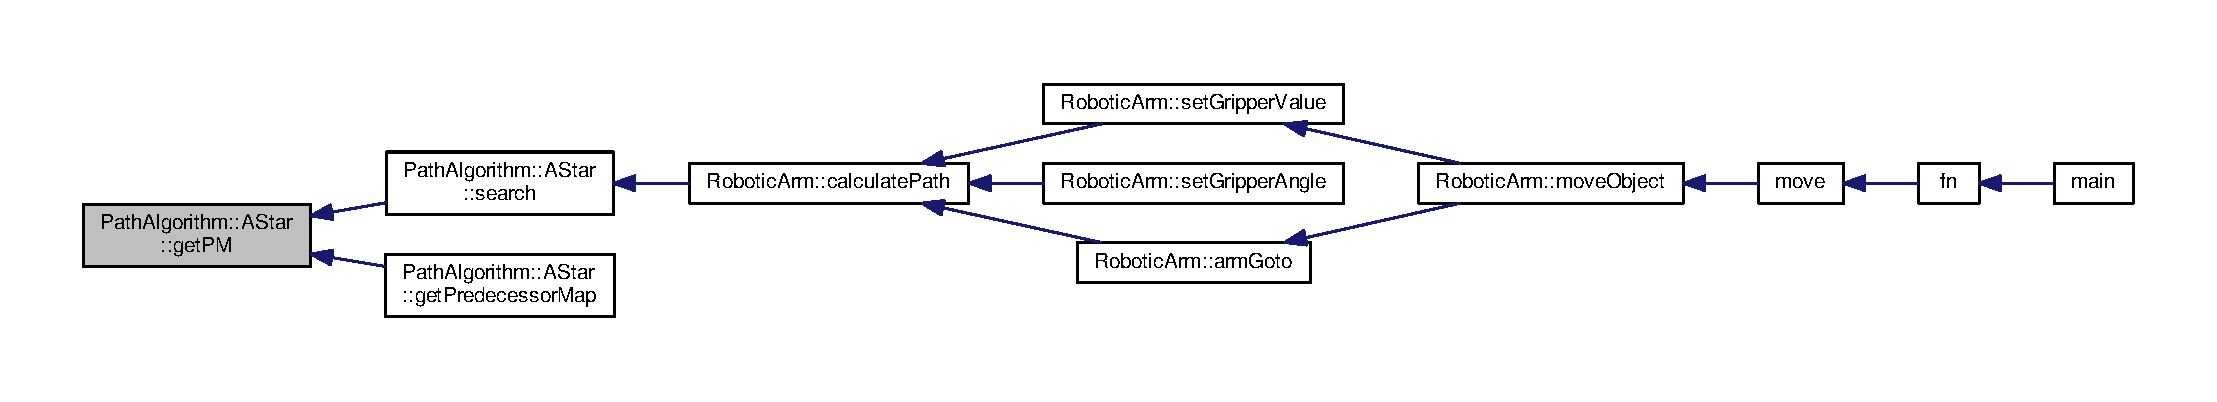
\includegraphics[width=350pt]{class_path_algorithm_1_1_a_star_a4bb6718fd07f503ff836c5cdccd74236_icgraph}
\end{center}
\end{figure}


\index{Path\+Algorithm\+::\+A\+Star@{Path\+Algorithm\+::\+A\+Star}!get\+PM@{get\+PM}}
\index{get\+PM@{get\+PM}!Path\+Algorithm\+::\+A\+Star@{Path\+Algorithm\+::\+A\+Star}}
\subsubsection[{\texorpdfstring{get\+P\+M() const }{getPM() const }}]{\setlength{\rightskip}{0pt plus 5cm}const {\bf Vertex\+Map} \& Path\+Algorithm\+::\+A\+Star\+::get\+PM (
\begin{DoxyParamCaption}
{}
\end{DoxyParamCaption}
) const\hspace{0.3cm}{\ttfamily [protected]}}\hypertarget{class_path_algorithm_1_1_a_star_a021ff514f018ce9ec7db705578a210d4}{}\label{class_path_algorithm_1_1_a_star_a021ff514f018ce9ec7db705578a210d4}


Definition at line 434 of file A\+Star.\+cpp.

\index{Path\+Algorithm\+::\+A\+Star@{Path\+Algorithm\+::\+A\+Star}!get\+Predecessor\+Map@{get\+Predecessor\+Map}}
\index{get\+Predecessor\+Map@{get\+Predecessor\+Map}!Path\+Algorithm\+::\+A\+Star@{Path\+Algorithm\+::\+A\+Star}}
\subsubsection[{\texorpdfstring{get\+Predecessor\+Map() const }{getPredecessorMap() const }}]{\setlength{\rightskip}{0pt plus 5cm}{\bf Vertex\+Map} Path\+Algorithm\+::\+A\+Star\+::get\+Predecessor\+Map (
\begin{DoxyParamCaption}
{}
\end{DoxyParamCaption}
) const}\hypertarget{class_path_algorithm_1_1_a_star_ac4ce233712c0f7aac44d029e61888581}{}\label{class_path_algorithm_1_1_a_star_ac4ce233712c0f7aac44d029e61888581}


Definition at line 384 of file A\+Star.\+cpp.



Here is the call graph for this function\+:\nopagebreak
\begin{figure}[H]
\begin{center}
\leavevmode
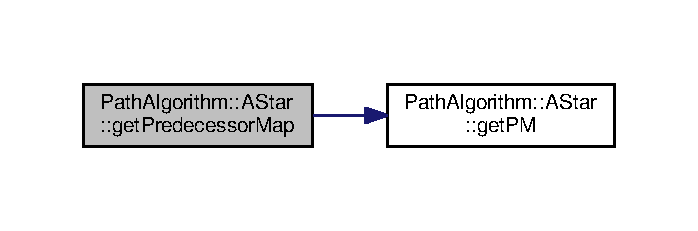
\includegraphics[width=335pt]{class_path_algorithm_1_1_a_star_ac4ce233712c0f7aac44d029e61888581_cgraph}
\end{center}
\end{figure}


\index{Path\+Algorithm\+::\+A\+Star@{Path\+Algorithm\+::\+A\+Star}!remove\+First\+From\+Open\+Set@{remove\+First\+From\+Open\+Set}}
\index{remove\+First\+From\+Open\+Set@{remove\+First\+From\+Open\+Set}!Path\+Algorithm\+::\+A\+Star@{Path\+Algorithm\+::\+A\+Star}}
\subsubsection[{\texorpdfstring{remove\+First\+From\+Open\+Set()}{removeFirstFromOpenSet()}}]{\setlength{\rightskip}{0pt plus 5cm}void Path\+Algorithm\+::\+A\+Star\+::remove\+First\+From\+Open\+Set (
\begin{DoxyParamCaption}
{}
\end{DoxyParamCaption}
)}\hypertarget{class_path_algorithm_1_1_a_star_a5bb18edbbd54833aac9eddfe63ba652d}{}\label{class_path_algorithm_1_1_a_star_a5bb18edbbd54833aac9eddfe63ba652d}


Definition at line 308 of file A\+Star.\+cpp.



Here is the caller graph for this function\+:\nopagebreak
\begin{figure}[H]
\begin{center}
\leavevmode
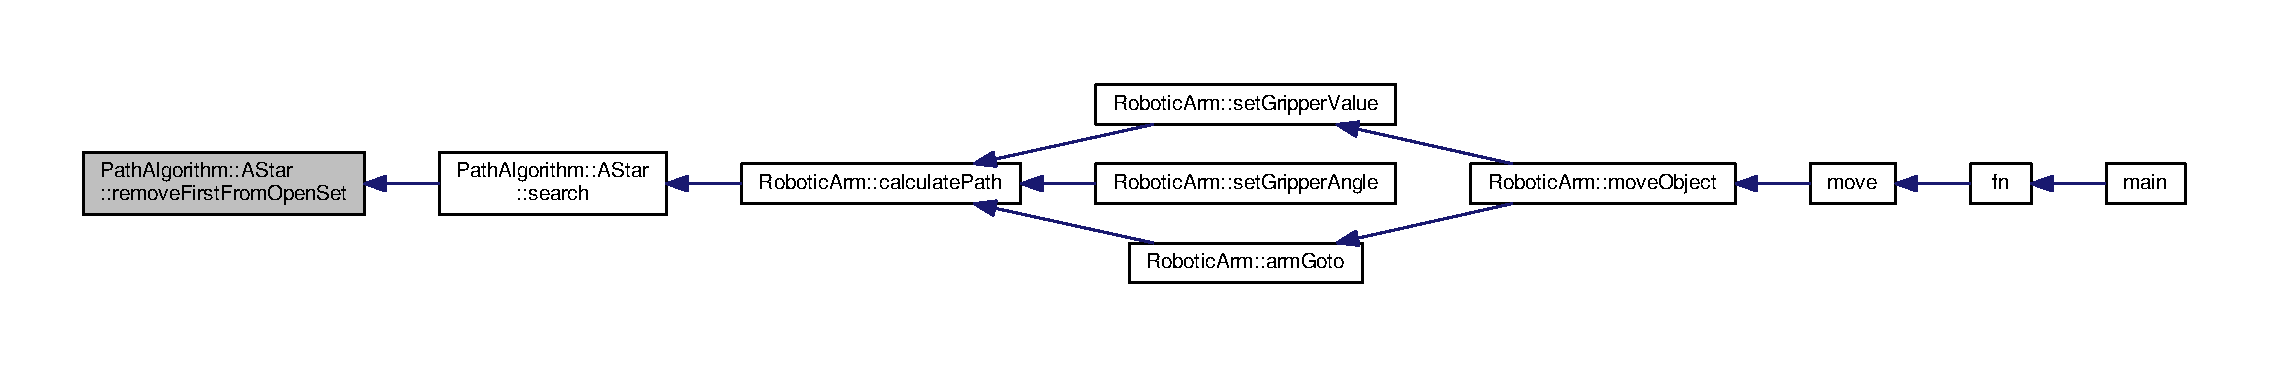
\includegraphics[width=350pt]{class_path_algorithm_1_1_a_star_a5bb18edbbd54833aac9eddfe63ba652d_icgraph}
\end{center}
\end{figure}


\index{Path\+Algorithm\+::\+A\+Star@{Path\+Algorithm\+::\+A\+Star}!remove\+From\+Closed\+Set@{remove\+From\+Closed\+Set}}
\index{remove\+From\+Closed\+Set@{remove\+From\+Closed\+Set}!Path\+Algorithm\+::\+A\+Star@{Path\+Algorithm\+::\+A\+Star}}
\subsubsection[{\texorpdfstring{remove\+From\+Closed\+Set(const Vertex \&a\+Vertex)}{removeFromClosedSet(const Vertex &aVertex)}}]{\setlength{\rightskip}{0pt plus 5cm}void Path\+Algorithm\+::\+A\+Star\+::remove\+From\+Closed\+Set (
\begin{DoxyParamCaption}
\item[{const {\bf Vertex} \&}]{a\+Vertex}
\end{DoxyParamCaption}
)}\hypertarget{class_path_algorithm_1_1_a_star_a1b6971a9c5878e859cbdb3270dda93b4}{}\label{class_path_algorithm_1_1_a_star_a1b6971a9c5878e859cbdb3270dda93b4}


Definition at line 325 of file A\+Star.\+cpp.



Here is the call graph for this function\+:\nopagebreak
\begin{figure}[H]
\begin{center}
\leavevmode
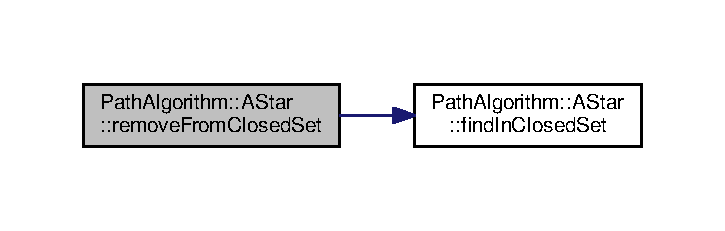
\includegraphics[width=348pt]{class_path_algorithm_1_1_a_star_a1b6971a9c5878e859cbdb3270dda93b4_cgraph}
\end{center}
\end{figure}




Here is the caller graph for this function\+:\nopagebreak
\begin{figure}[H]
\begin{center}
\leavevmode
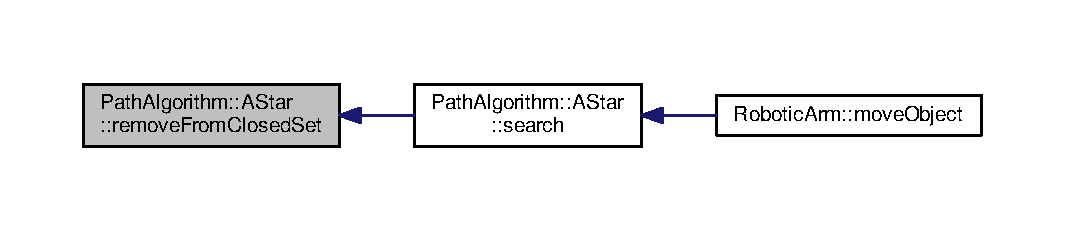
\includegraphics[width=350pt]{class_path_algorithm_1_1_a_star_a1b6971a9c5878e859cbdb3270dda93b4_icgraph}
\end{center}
\end{figure}


\index{Path\+Algorithm\+::\+A\+Star@{Path\+Algorithm\+::\+A\+Star}!remove\+From\+Closed\+Set@{remove\+From\+Closed\+Set}}
\index{remove\+From\+Closed\+Set@{remove\+From\+Closed\+Set}!Path\+Algorithm\+::\+A\+Star@{Path\+Algorithm\+::\+A\+Star}}
\subsubsection[{\texorpdfstring{remove\+From\+Closed\+Set(\+Closed\+Set\+::iterator \&i)}{removeFromClosedSet(ClosedSet::iterator &i)}}]{\setlength{\rightskip}{0pt plus 5cm}void Path\+Algorithm\+::\+A\+Star\+::remove\+From\+Closed\+Set (
\begin{DoxyParamCaption}
\item[{Closed\+Set\+::iterator \&}]{i}
\end{DoxyParamCaption}
)}\hypertarget{class_path_algorithm_1_1_a_star_a799953993c1255f0ce559f7233d3c926}{}\label{class_path_algorithm_1_1_a_star_a799953993c1255f0ce559f7233d3c926}


Definition at line 334 of file A\+Star.\+cpp.

\index{Path\+Algorithm\+::\+A\+Star@{Path\+Algorithm\+::\+A\+Star}!remove\+From\+Open\+Set@{remove\+From\+Open\+Set}}
\index{remove\+From\+Open\+Set@{remove\+From\+Open\+Set}!Path\+Algorithm\+::\+A\+Star@{Path\+Algorithm\+::\+A\+Star}}
\subsubsection[{\texorpdfstring{remove\+From\+Open\+Set(const Vertex \&a\+Vertex)}{removeFromOpenSet(const Vertex &aVertex)}}]{\setlength{\rightskip}{0pt plus 5cm}void Path\+Algorithm\+::\+A\+Star\+::remove\+From\+Open\+Set (
\begin{DoxyParamCaption}
\item[{const {\bf Vertex} \&}]{a\+Vertex}
\end{DoxyParamCaption}
)}\hypertarget{class_path_algorithm_1_1_a_star_afcc23a676145d6e280d1c3430af5380a}{}\label{class_path_algorithm_1_1_a_star_afcc23a676145d6e280d1c3430af5380a}


Definition at line 264 of file A\+Star.\+cpp.



Here is the call graph for this function\+:\nopagebreak
\begin{figure}[H]
\begin{center}
\leavevmode
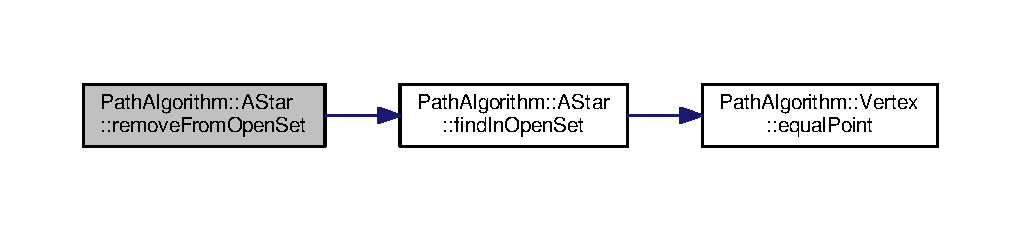
\includegraphics[width=350pt]{class_path_algorithm_1_1_a_star_afcc23a676145d6e280d1c3430af5380a_cgraph}
\end{center}
\end{figure}




Here is the caller graph for this function\+:\nopagebreak
\begin{figure}[H]
\begin{center}
\leavevmode
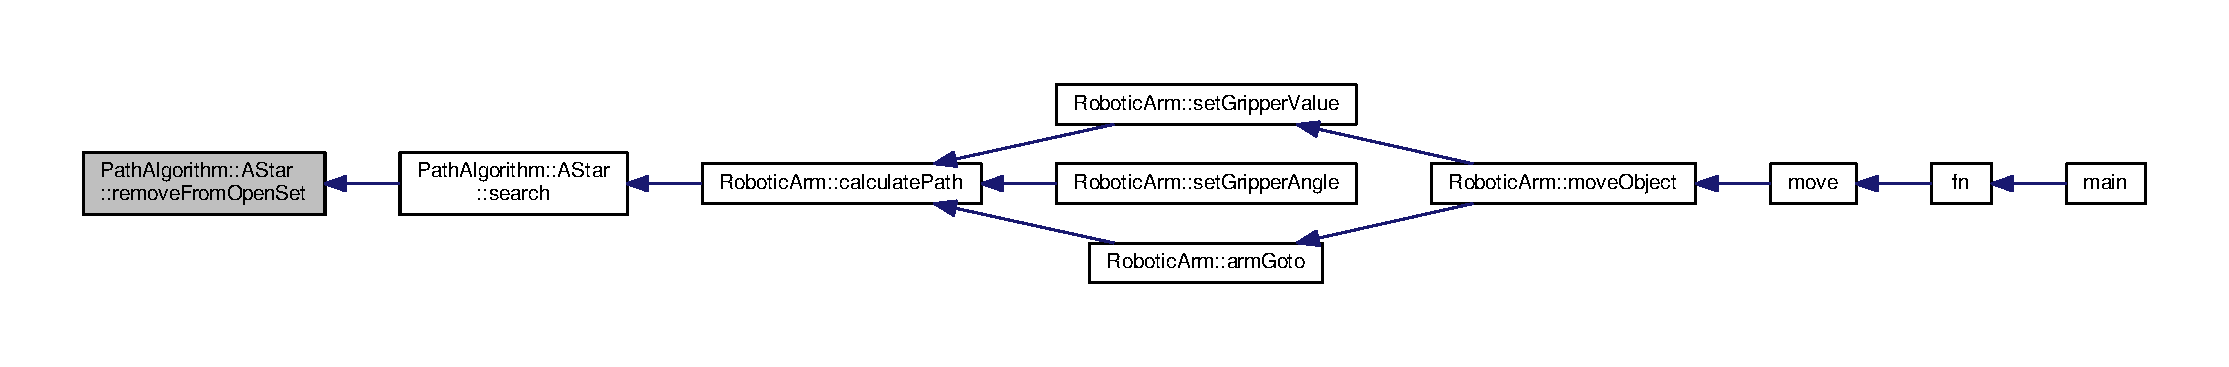
\includegraphics[width=350pt]{class_path_algorithm_1_1_a_star_afcc23a676145d6e280d1c3430af5380a_icgraph}
\end{center}
\end{figure}


\index{Path\+Algorithm\+::\+A\+Star@{Path\+Algorithm\+::\+A\+Star}!remove\+From\+Open\+Set@{remove\+From\+Open\+Set}}
\index{remove\+From\+Open\+Set@{remove\+From\+Open\+Set}!Path\+Algorithm\+::\+A\+Star@{Path\+Algorithm\+::\+A\+Star}}
\subsubsection[{\texorpdfstring{remove\+From\+Open\+Set(\+Open\+Set\+::iterator \&i)}{removeFromOpenSet(OpenSet::iterator &i)}}]{\setlength{\rightskip}{0pt plus 5cm}void Path\+Algorithm\+::\+A\+Star\+::remove\+From\+Open\+Set (
\begin{DoxyParamCaption}
\item[{Open\+Set\+::iterator \&}]{i}
\end{DoxyParamCaption}
)}\hypertarget{class_path_algorithm_1_1_a_star_aba29c2585fbf49880cf5e8b9bf6d3eb5}{}\label{class_path_algorithm_1_1_a_star_aba29c2585fbf49880cf5e8b9bf6d3eb5}


Definition at line 273 of file A\+Star.\+cpp.

\index{Path\+Algorithm\+::\+A\+Star@{Path\+Algorithm\+::\+A\+Star}!search@{search}}
\index{search@{search}!Path\+Algorithm\+::\+A\+Star@{Path\+Algorithm\+::\+A\+Star}}
\subsubsection[{\texorpdfstring{search(\+Vertex a\+Start, const Vertex \&a\+Goal, const Size \&a\+Robot\+Size, Robotic\+Arm \&robot)}{search(Vertex aStart, const Vertex &aGoal, const Size &aRobotSize, RoboticArm &robot)}}]{\setlength{\rightskip}{0pt plus 5cm}{\bf Path} Path\+Algorithm\+::\+A\+Star\+::search (
\begin{DoxyParamCaption}
\item[{{\bf Vertex}}]{a\+Start, }
\item[{const {\bf Vertex} \&}]{a\+Goal, }
\item[{const {\bf Size} \&}]{a\+Robot\+Size, }
\item[{{\bf Robotic\+Arm} \&}]{robot}
\end{DoxyParamCaption}
)}\hypertarget{class_path_algorithm_1_1_a_star_aee41b31ec44b02f6dc94889d228a3582}{}\label{class_path_algorithm_1_1_a_star_aee41b31ec44b02f6dc94889d228a3582}


Definition at line 100 of file A\+Star.\+cpp.



Here is the call graph for this function\+:\nopagebreak
\begin{figure}[H]
\begin{center}
\leavevmode
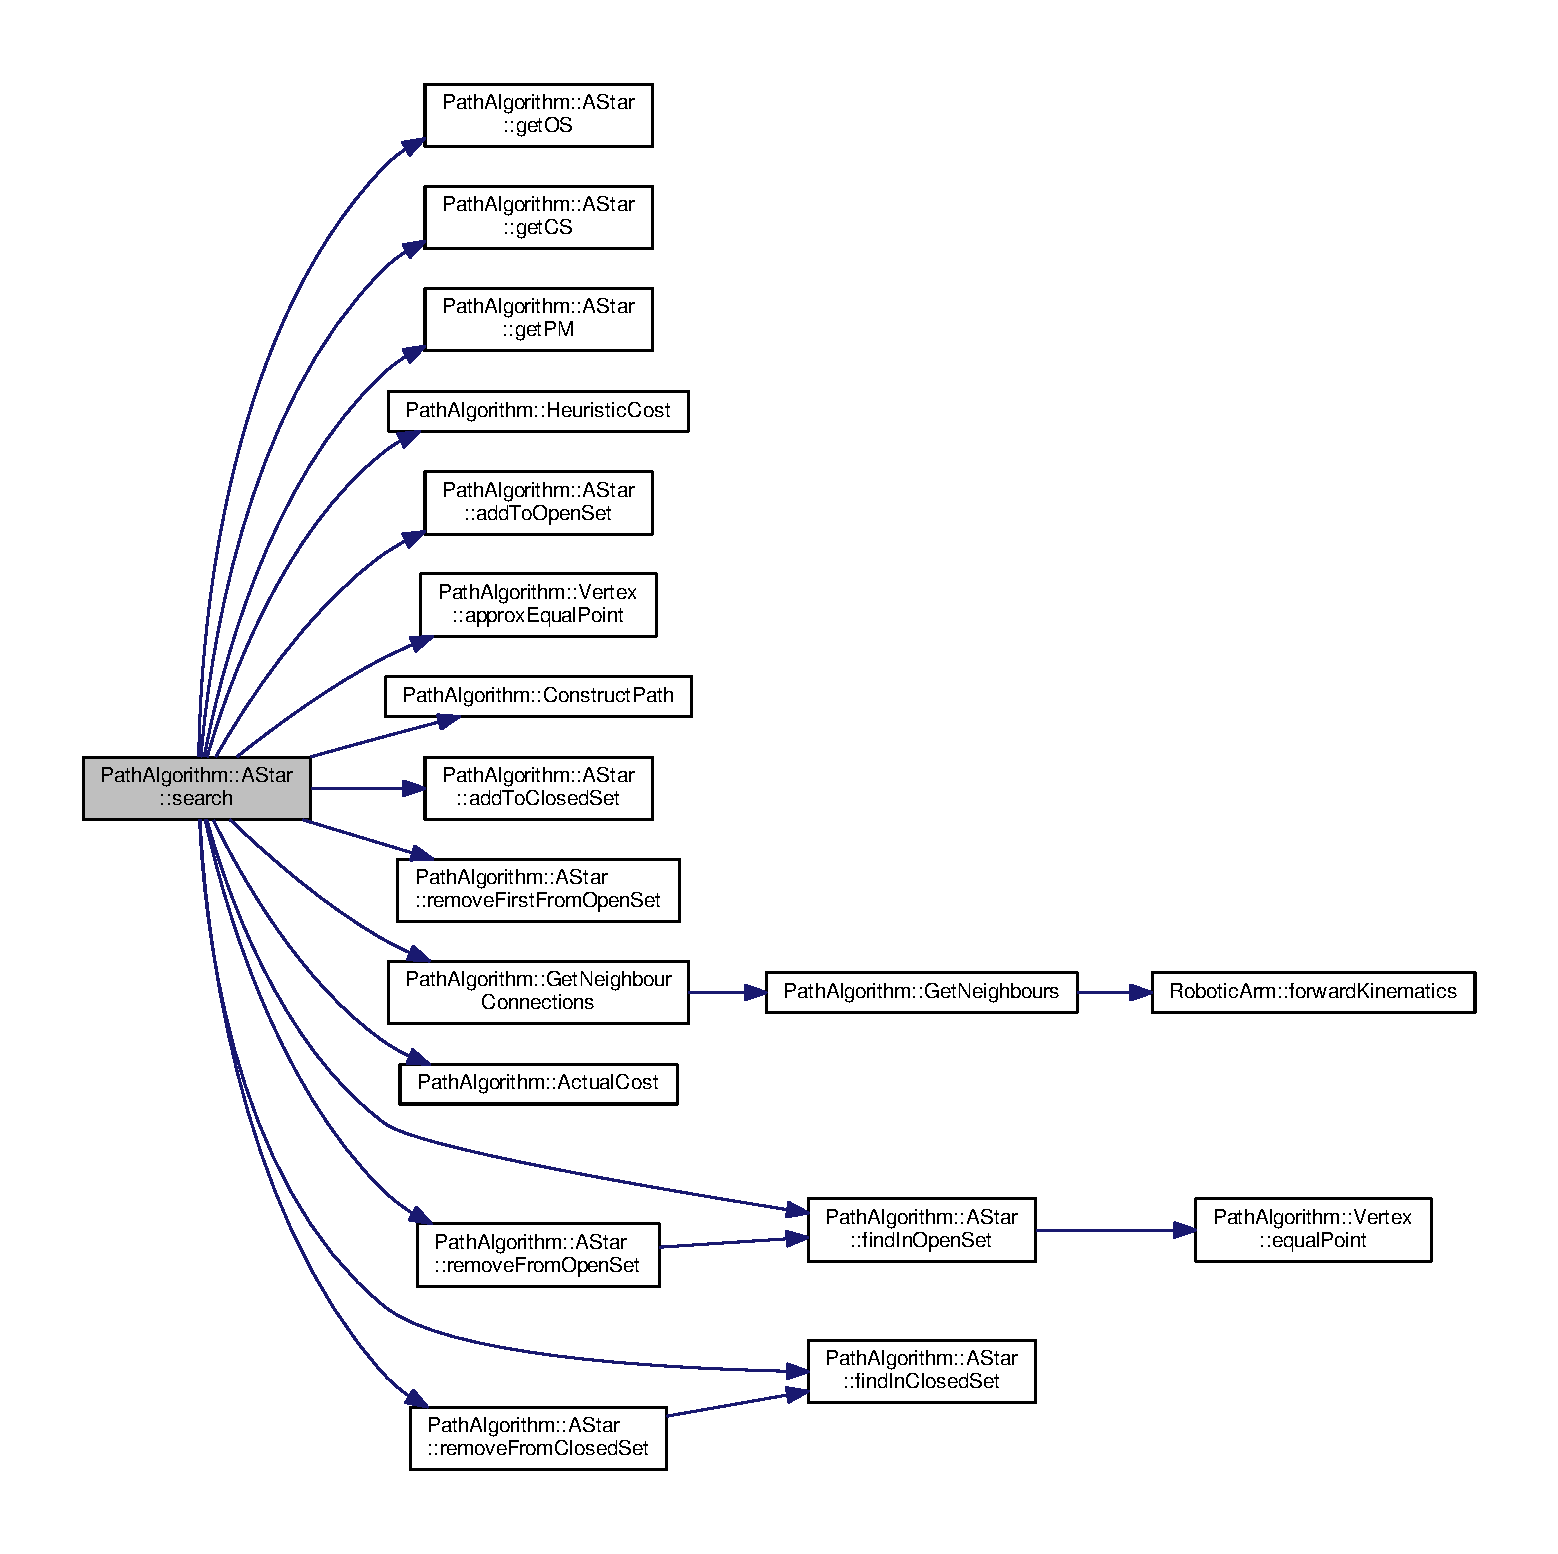
\includegraphics[width=350pt]{class_path_algorithm_1_1_a_star_aee41b31ec44b02f6dc94889d228a3582_cgraph}
\end{center}
\end{figure}




Here is the caller graph for this function\+:\nopagebreak
\begin{figure}[H]
\begin{center}
\leavevmode
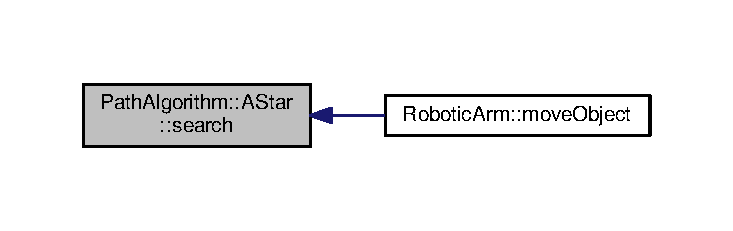
\includegraphics[width=350pt]{class_path_algorithm_1_1_a_star_aee41b31ec44b02f6dc94889d228a3582_icgraph}
\end{center}
\end{figure}




The documentation for this class was generated from the following files\+:\begin{DoxyCompactItemize}
\item 
src/\hyperlink{_a_star_8hpp}{A\+Star.\+hpp}\item 
src/\hyperlink{_a_star_8cpp}{A\+Star.\+cpp}\end{DoxyCompactItemize}

\hypertarget{struct_colour}{}\section{Colour Struct Reference}
\label{struct_colour}\index{Colour@{Colour}}


Struct for the colour thresholds.  




{\ttfamily \#include $<$vision.\+hpp$>$}



Collaboration diagram for Colour\+:\nopagebreak
\begin{figure}[H]
\begin{center}
\leavevmode
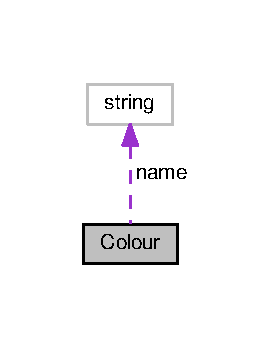
\includegraphics[width=131pt]{struct_colour__coll__graph}
\end{center}
\end{figure}
\subsection*{Public Attributes}
\begin{DoxyCompactItemize}
\item 
int \hyperlink{struct_colour_ad80795d6cb069ebb1ba58d21dc431a1f}{hue\+\_\+min}
\item 
int \hyperlink{struct_colour_a060d31cb0c6cd91881d3b194878ecc9c}{sat\+\_\+min}
\item 
int \hyperlink{struct_colour_ac9491a53fac7ac1d76a3a0fb3845ac18}{val\+\_\+min}
\item 
int \hyperlink{struct_colour_ad5bb23b460d5d34079ae34e7e1c0940c}{hue\+\_\+max}
\item 
int \hyperlink{struct_colour_afe350ccf1ecf2dbf5f414ba869878d65}{sat\+\_\+max}
\item 
int \hyperlink{struct_colour_abc073c89d95297937d9743f52170e853}{val\+\_\+max}
\item 
string \hyperlink{struct_colour_a4a7225c84050a0d8d9164643a0ccbbd2}{name}
\end{DoxyCompactItemize}


\subsection{Detailed Description}
Struct for the colour thresholds. 


\begin{DoxyParams}{Parameters}
{\em hue\+\_\+min} & the minimal hue \\
\hline
{\em sat\+\_\+min} & the minimal saturation \\
\hline
{\em val\+\_\+min} & the minimal value \\
\hline
{\em hue\+\_\+max} & the maximal hue \\
\hline
{\em sat\+\_\+max} & the maximal saturation \\
\hline
{\em val\+\_\+max} & the maximal value \\
\hline
\end{DoxyParams}


Definition at line 34 of file vision.\+hpp.



\subsection{Member Data Documentation}
\index{Colour@{Colour}!hue\+\_\+max@{hue\+\_\+max}}
\index{hue\+\_\+max@{hue\+\_\+max}!Colour@{Colour}}
\subsubsection[{\texorpdfstring{hue\+\_\+max}{hue_max}}]{\setlength{\rightskip}{0pt plus 5cm}int Colour\+::hue\+\_\+max}\hypertarget{struct_colour_ad5bb23b460d5d34079ae34e7e1c0940c}{}\label{struct_colour_ad5bb23b460d5d34079ae34e7e1c0940c}


Definition at line 39 of file vision.\+hpp.

\index{Colour@{Colour}!hue\+\_\+min@{hue\+\_\+min}}
\index{hue\+\_\+min@{hue\+\_\+min}!Colour@{Colour}}
\subsubsection[{\texorpdfstring{hue\+\_\+min}{hue_min}}]{\setlength{\rightskip}{0pt plus 5cm}int Colour\+::hue\+\_\+min}\hypertarget{struct_colour_ad80795d6cb069ebb1ba58d21dc431a1f}{}\label{struct_colour_ad80795d6cb069ebb1ba58d21dc431a1f}


Definition at line 36 of file vision.\+hpp.

\index{Colour@{Colour}!name@{name}}
\index{name@{name}!Colour@{Colour}}
\subsubsection[{\texorpdfstring{name}{name}}]{\setlength{\rightskip}{0pt plus 5cm}string Colour\+::name}\hypertarget{struct_colour_a4a7225c84050a0d8d9164643a0ccbbd2}{}\label{struct_colour_a4a7225c84050a0d8d9164643a0ccbbd2}


Definition at line 42 of file vision.\+hpp.

\index{Colour@{Colour}!sat\+\_\+max@{sat\+\_\+max}}
\index{sat\+\_\+max@{sat\+\_\+max}!Colour@{Colour}}
\subsubsection[{\texorpdfstring{sat\+\_\+max}{sat_max}}]{\setlength{\rightskip}{0pt plus 5cm}int Colour\+::sat\+\_\+max}\hypertarget{struct_colour_afe350ccf1ecf2dbf5f414ba869878d65}{}\label{struct_colour_afe350ccf1ecf2dbf5f414ba869878d65}


Definition at line 40 of file vision.\+hpp.

\index{Colour@{Colour}!sat\+\_\+min@{sat\+\_\+min}}
\index{sat\+\_\+min@{sat\+\_\+min}!Colour@{Colour}}
\subsubsection[{\texorpdfstring{sat\+\_\+min}{sat_min}}]{\setlength{\rightskip}{0pt plus 5cm}int Colour\+::sat\+\_\+min}\hypertarget{struct_colour_a060d31cb0c6cd91881d3b194878ecc9c}{}\label{struct_colour_a060d31cb0c6cd91881d3b194878ecc9c}


Definition at line 37 of file vision.\+hpp.

\index{Colour@{Colour}!val\+\_\+max@{val\+\_\+max}}
\index{val\+\_\+max@{val\+\_\+max}!Colour@{Colour}}
\subsubsection[{\texorpdfstring{val\+\_\+max}{val_max}}]{\setlength{\rightskip}{0pt plus 5cm}int Colour\+::val\+\_\+max}\hypertarget{struct_colour_abc073c89d95297937d9743f52170e853}{}\label{struct_colour_abc073c89d95297937d9743f52170e853}


Definition at line 41 of file vision.\+hpp.

\index{Colour@{Colour}!val\+\_\+min@{val\+\_\+min}}
\index{val\+\_\+min@{val\+\_\+min}!Colour@{Colour}}
\subsubsection[{\texorpdfstring{val\+\_\+min}{val_min}}]{\setlength{\rightskip}{0pt plus 5cm}int Colour\+::val\+\_\+min}\hypertarget{struct_colour_ac9491a53fac7ac1d76a3a0fb3845ac18}{}\label{struct_colour_ac9491a53fac7ac1d76a3a0fb3845ac18}


Definition at line 38 of file vision.\+hpp.



The documentation for this struct was generated from the following file\+:\begin{DoxyCompactItemize}
\item 
src/\hyperlink{vision_8hpp}{vision.\+hpp}\end{DoxyCompactItemize}

\hypertarget{struct_path_algorithm_1_1_edge}{}\section{Path\+Algorithm\+:\+:Edge Struct Reference}
\label{struct_path_algorithm_1_1_edge}\index{Path\+Algorithm\+::\+Edge@{Path\+Algorithm\+::\+Edge}}


{\ttfamily \#include $<$A\+Star.\+hpp$>$}



Collaboration diagram for Path\+Algorithm\+:\+:Edge\+:\nopagebreak
\begin{figure}[H]
\begin{center}
\leavevmode
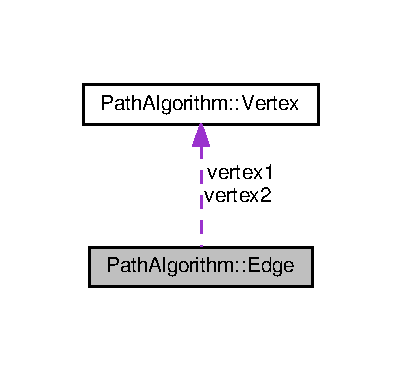
\includegraphics[width=193pt]{struct_path_algorithm_1_1_edge__coll__graph}
\end{center}
\end{figure}
\subsection*{Public Member Functions}
\begin{DoxyCompactItemize}
\item 
\hyperlink{struct_path_algorithm_1_1_edge_a4378105bc5d8b8b2fd147cb8b5a62662}{Edge} (const \hyperlink{struct_path_algorithm_1_1_vertex}{Vertex} \&a\+Vertex1, const \hyperlink{struct_path_algorithm_1_1_vertex}{Vertex} \&a\+Vertex2)
\item 
\hyperlink{struct_path_algorithm_1_1_edge_a2a1cfa63c51fac6e9c7385ab6b0b0b0c}{Edge} (const \hyperlink{struct_path_algorithm_1_1_edge}{Edge} \&an\+Edge)
\item 
const \hyperlink{struct_path_algorithm_1_1_vertex}{Vertex} \& \hyperlink{struct_path_algorithm_1_1_edge_a0a987c8705e5e41f890fb4f222243af8}{this\+Side} (const \hyperlink{struct_path_algorithm_1_1_vertex}{Vertex} \&a\+Vertex) const 
\item 
const \hyperlink{struct_path_algorithm_1_1_vertex}{Vertex} \& \hyperlink{struct_path_algorithm_1_1_edge_a204de7bc294af2cd5df73c29b2587345}{other\+Side} (const \hyperlink{struct_path_algorithm_1_1_vertex}{Vertex} \&a\+Vertex) const 
\end{DoxyCompactItemize}
\subsection*{Public Attributes}
\begin{DoxyCompactItemize}
\item 
\hyperlink{struct_path_algorithm_1_1_vertex}{Vertex} \hyperlink{struct_path_algorithm_1_1_edge_ab655d5ef6c7022bc87520c4e751b4dcf}{vertex1}
\item 
\hyperlink{struct_path_algorithm_1_1_vertex}{Vertex} \hyperlink{struct_path_algorithm_1_1_edge_ab8d28fabc8b10986f4e4d915f0b6f16a}{vertex2}
\end{DoxyCompactItemize}


\subsection{Detailed Description}


Definition at line 134 of file A\+Star.\+hpp.



\subsection{Constructor \& Destructor Documentation}
\index{Path\+Algorithm\+::\+Edge@{Path\+Algorithm\+::\+Edge}!Edge@{Edge}}
\index{Edge@{Edge}!Path\+Algorithm\+::\+Edge@{Path\+Algorithm\+::\+Edge}}
\subsubsection[{\texorpdfstring{Edge(const Vertex \&a\+Vertex1, const Vertex \&a\+Vertex2)}{Edge(const Vertex &aVertex1, const Vertex &aVertex2)}}]{\setlength{\rightskip}{0pt plus 5cm}Path\+Algorithm\+::\+Edge\+::\+Edge (
\begin{DoxyParamCaption}
\item[{const {\bf Vertex} \&}]{a\+Vertex1, }
\item[{const {\bf Vertex} \&}]{a\+Vertex2}
\end{DoxyParamCaption}
)\hspace{0.3cm}{\ttfamily [inline]}}\hypertarget{struct_path_algorithm_1_1_edge_a4378105bc5d8b8b2fd147cb8b5a62662}{}\label{struct_path_algorithm_1_1_edge_a4378105bc5d8b8b2fd147cb8b5a62662}


Definition at line 136 of file A\+Star.\+hpp.

\index{Path\+Algorithm\+::\+Edge@{Path\+Algorithm\+::\+Edge}!Edge@{Edge}}
\index{Edge@{Edge}!Path\+Algorithm\+::\+Edge@{Path\+Algorithm\+::\+Edge}}
\subsubsection[{\texorpdfstring{Edge(const Edge \&an\+Edge)}{Edge(const Edge &anEdge)}}]{\setlength{\rightskip}{0pt plus 5cm}Path\+Algorithm\+::\+Edge\+::\+Edge (
\begin{DoxyParamCaption}
\item[{const {\bf Edge} \&}]{an\+Edge}
\end{DoxyParamCaption}
)\hspace{0.3cm}{\ttfamily [inline]}}\hypertarget{struct_path_algorithm_1_1_edge_a2a1cfa63c51fac6e9c7385ab6b0b0b0c}{}\label{struct_path_algorithm_1_1_edge_a2a1cfa63c51fac6e9c7385ab6b0b0b0c}


Definition at line 140 of file A\+Star.\+hpp.



\subsection{Member Function Documentation}
\index{Path\+Algorithm\+::\+Edge@{Path\+Algorithm\+::\+Edge}!other\+Side@{other\+Side}}
\index{other\+Side@{other\+Side}!Path\+Algorithm\+::\+Edge@{Path\+Algorithm\+::\+Edge}}
\subsubsection[{\texorpdfstring{other\+Side(const Vertex \&a\+Vertex) const }{otherSide(const Vertex &aVertex) const }}]{\setlength{\rightskip}{0pt plus 5cm}const {\bf Vertex}\& Path\+Algorithm\+::\+Edge\+::other\+Side (
\begin{DoxyParamCaption}
\item[{const {\bf Vertex} \&}]{a\+Vertex}
\end{DoxyParamCaption}
) const\hspace{0.3cm}{\ttfamily [inline]}}\hypertarget{struct_path_algorithm_1_1_edge_a204de7bc294af2cd5df73c29b2587345}{}\label{struct_path_algorithm_1_1_edge_a204de7bc294af2cd5df73c29b2587345}


Definition at line 154 of file A\+Star.\+hpp.

\index{Path\+Algorithm\+::\+Edge@{Path\+Algorithm\+::\+Edge}!this\+Side@{this\+Side}}
\index{this\+Side@{this\+Side}!Path\+Algorithm\+::\+Edge@{Path\+Algorithm\+::\+Edge}}
\subsubsection[{\texorpdfstring{this\+Side(const Vertex \&a\+Vertex) const }{thisSide(const Vertex &aVertex) const }}]{\setlength{\rightskip}{0pt plus 5cm}const {\bf Vertex}\& Path\+Algorithm\+::\+Edge\+::this\+Side (
\begin{DoxyParamCaption}
\item[{const {\bf Vertex} \&}]{a\+Vertex}
\end{DoxyParamCaption}
) const\hspace{0.3cm}{\ttfamily [inline]}}\hypertarget{struct_path_algorithm_1_1_edge_a0a987c8705e5e41f890fb4f222243af8}{}\label{struct_path_algorithm_1_1_edge_a0a987c8705e5e41f890fb4f222243af8}


Definition at line 145 of file A\+Star.\+hpp.



\subsection{Member Data Documentation}
\index{Path\+Algorithm\+::\+Edge@{Path\+Algorithm\+::\+Edge}!vertex1@{vertex1}}
\index{vertex1@{vertex1}!Path\+Algorithm\+::\+Edge@{Path\+Algorithm\+::\+Edge}}
\subsubsection[{\texorpdfstring{vertex1}{vertex1}}]{\setlength{\rightskip}{0pt plus 5cm}{\bf Vertex} Path\+Algorithm\+::\+Edge\+::vertex1}\hypertarget{struct_path_algorithm_1_1_edge_ab655d5ef6c7022bc87520c4e751b4dcf}{}\label{struct_path_algorithm_1_1_edge_ab655d5ef6c7022bc87520c4e751b4dcf}


Definition at line 163 of file A\+Star.\+hpp.

\index{Path\+Algorithm\+::\+Edge@{Path\+Algorithm\+::\+Edge}!vertex2@{vertex2}}
\index{vertex2@{vertex2}!Path\+Algorithm\+::\+Edge@{Path\+Algorithm\+::\+Edge}}
\subsubsection[{\texorpdfstring{vertex2}{vertex2}}]{\setlength{\rightskip}{0pt plus 5cm}{\bf Vertex} Path\+Algorithm\+::\+Edge\+::vertex2}\hypertarget{struct_path_algorithm_1_1_edge_ab8d28fabc8b10986f4e4d915f0b6f16a}{}\label{struct_path_algorithm_1_1_edge_ab8d28fabc8b10986f4e4d915f0b6f16a}


Definition at line 164 of file A\+Star.\+hpp.



The documentation for this struct was generated from the following file\+:\begin{DoxyCompactItemize}
\item 
src/\hyperlink{_a_star_8hpp}{A\+Star.\+hpp}\end{DoxyCompactItemize}

\hypertarget{struct_path_algorithm_1_1_graph}{}\section{Path\+Algorithm\+:\+:Graph Struct Reference}
\label{struct_path_algorithm_1_1_graph}\index{Path\+Algorithm\+::\+Graph@{Path\+Algorithm\+::\+Graph}}


{\ttfamily \#include $<$A\+Star.\+hpp$>$}

\subsection*{Public Member Functions}
\begin{DoxyCompactItemize}
\item 
void \hyperlink{struct_path_algorithm_1_1_graph_a185d5e83f65e20c5549169a1f8c2c6e6}{setE} (\hyperlink{struct_path_algorithm_1_1_edge}{Edge} \hyperlink{struct_path_algorithm_1_1_graph_a74823a65650b0f20268b0a274a2b69a7}{e})
\item 
void \hyperlink{struct_path_algorithm_1_1_graph_a7754a1020f2d394070f7cdf63ba1e446}{setV} (\hyperlink{struct_path_algorithm_1_1_vertex}{Vertex} \hyperlink{struct_path_algorithm_1_1_graph_a8c71f9d9965684ae31ab85ccec9c8114}{v})
\end{DoxyCompactItemize}
\subsection*{Static Public Member Functions}
\begin{DoxyCompactItemize}
\item 
static \hyperlink{struct_path_algorithm_1_1_graph}{Graph} \& \hyperlink{struct_path_algorithm_1_1_graph_ab9015f34eac8789354a91091630fbbe9}{get\+Instance} ()
\end{DoxyCompactItemize}
\subsection*{Public Attributes}
\begin{DoxyCompactItemize}
\item 
std\+::vector$<$ \hyperlink{struct_path_algorithm_1_1_edge}{Edge} $>$ \hyperlink{struct_path_algorithm_1_1_graph_a74823a65650b0f20268b0a274a2b69a7}{e}
\item 
std\+::vector$<$ \hyperlink{struct_path_algorithm_1_1_vertex}{Vertex} $>$ \hyperlink{struct_path_algorithm_1_1_graph_a8c71f9d9965684ae31ab85ccec9c8114}{v}
\end{DoxyCompactItemize}


\subsection{Detailed Description}


Definition at line 308 of file A\+Star.\+hpp.



\subsection{Member Function Documentation}
\index{Path\+Algorithm\+::\+Graph@{Path\+Algorithm\+::\+Graph}!get\+Instance@{get\+Instance}}
\index{get\+Instance@{get\+Instance}!Path\+Algorithm\+::\+Graph@{Path\+Algorithm\+::\+Graph}}
\subsubsection[{\texorpdfstring{get\+Instance()}{getInstance()}}]{\setlength{\rightskip}{0pt plus 5cm}static {\bf Graph}\& Path\+Algorithm\+::\+Graph\+::get\+Instance (
\begin{DoxyParamCaption}
{}
\end{DoxyParamCaption}
)\hspace{0.3cm}{\ttfamily [inline]}, {\ttfamily [static]}}\hypertarget{struct_path_algorithm_1_1_graph_ab9015f34eac8789354a91091630fbbe9}{}\label{struct_path_algorithm_1_1_graph_ab9015f34eac8789354a91091630fbbe9}


Definition at line 312 of file A\+Star.\+hpp.

\index{Path\+Algorithm\+::\+Graph@{Path\+Algorithm\+::\+Graph}!setE@{setE}}
\index{setE@{setE}!Path\+Algorithm\+::\+Graph@{Path\+Algorithm\+::\+Graph}}
\subsubsection[{\texorpdfstring{set\+E(\+Edge e)}{setE(Edge e)}}]{\setlength{\rightskip}{0pt plus 5cm}void Path\+Algorithm\+::\+Graph\+::setE (
\begin{DoxyParamCaption}
\item[{{\bf Edge}}]{e}
\end{DoxyParamCaption}
)\hspace{0.3cm}{\ttfamily [inline]}}\hypertarget{struct_path_algorithm_1_1_graph_a185d5e83f65e20c5549169a1f8c2c6e6}{}\label{struct_path_algorithm_1_1_graph_a185d5e83f65e20c5549169a1f8c2c6e6}


Definition at line 317 of file A\+Star.\+hpp.

\index{Path\+Algorithm\+::\+Graph@{Path\+Algorithm\+::\+Graph}!setV@{setV}}
\index{setV@{setV}!Path\+Algorithm\+::\+Graph@{Path\+Algorithm\+::\+Graph}}
\subsubsection[{\texorpdfstring{set\+V(\+Vertex v)}{setV(Vertex v)}}]{\setlength{\rightskip}{0pt plus 5cm}void Path\+Algorithm\+::\+Graph\+::setV (
\begin{DoxyParamCaption}
\item[{{\bf Vertex}}]{v}
\end{DoxyParamCaption}
)\hspace{0.3cm}{\ttfamily [inline]}}\hypertarget{struct_path_algorithm_1_1_graph_a7754a1020f2d394070f7cdf63ba1e446}{}\label{struct_path_algorithm_1_1_graph_a7754a1020f2d394070f7cdf63ba1e446}


Definition at line 321 of file A\+Star.\+hpp.



\subsection{Member Data Documentation}
\index{Path\+Algorithm\+::\+Graph@{Path\+Algorithm\+::\+Graph}!e@{e}}
\index{e@{e}!Path\+Algorithm\+::\+Graph@{Path\+Algorithm\+::\+Graph}}
\subsubsection[{\texorpdfstring{e}{e}}]{\setlength{\rightskip}{0pt plus 5cm}std\+::vector$<${\bf Edge}$>$ Path\+Algorithm\+::\+Graph\+::e}\hypertarget{struct_path_algorithm_1_1_graph_a74823a65650b0f20268b0a274a2b69a7}{}\label{struct_path_algorithm_1_1_graph_a74823a65650b0f20268b0a274a2b69a7}


Definition at line 325 of file A\+Star.\+hpp.

\index{Path\+Algorithm\+::\+Graph@{Path\+Algorithm\+::\+Graph}!v@{v}}
\index{v@{v}!Path\+Algorithm\+::\+Graph@{Path\+Algorithm\+::\+Graph}}
\subsubsection[{\texorpdfstring{v}{v}}]{\setlength{\rightskip}{0pt plus 5cm}std\+::vector$<${\bf Vertex}$>$ Path\+Algorithm\+::\+Graph\+::v}\hypertarget{struct_path_algorithm_1_1_graph_a8c71f9d9965684ae31ab85ccec9c8114}{}\label{struct_path_algorithm_1_1_graph_a8c71f9d9965684ae31ab85ccec9c8114}


Definition at line 326 of file A\+Star.\+hpp.



The documentation for this struct was generated from the following file\+:\begin{DoxyCompactItemize}
\item 
src/\hyperlink{_a_star_8hpp}{A\+Star.\+hpp}\end{DoxyCompactItemize}

\hypertarget{class_interface}{}\section{Interface Class Reference}
\label{class_interface}\index{Interface@{Interface}}


{\ttfamily \#include $<$interface.\+hpp$>$}

\subsection*{Public Member Functions}
\begin{DoxyCompactItemize}
\item 
\hyperlink{class_interface_a4406d74c75bdfe150bf72be1f1cda8b1}{Interface} ()
\begin{DoxyCompactList}\small\item\em Constructor. \end{DoxyCompactList}\item 
\hyperlink{class_interface_a19179888f29f18f1be54a3dfe98f68c0}{$\sim$\+Interface} ()
\begin{DoxyCompactList}\small\item\em Destructor. \end{DoxyCompactList}\item 
int8\+\_\+t \hyperlink{class_interface_a345faa7570aa36a31681ca850d1c283d}{parser} (bool first\+\_\+time)
\begin{DoxyCompactList}\small\item\em Function that will read the input and will then check if it is correct and translate the input to a pair filled with the choices of the user. It calls. \end{DoxyCompactList}\item 
int8\+\_\+t \hyperlink{class_interface_a24b944dc66cb79f76ba91192a2a2860e}{await\+\_\+input} (bool first\+\_\+time)
\begin{DoxyCompactList}\small\item\em This function will serve the user a form to fill in and will call the parser function afterwards. \end{DoxyCompactList}\item 
uint8\+\_\+t \hyperlink{class_interface_adfa71e85801e5bb0e8bc88da902f8133}{get\+\_\+specification} () const 
\begin{DoxyCompactList}\small\item\em getter for the specification. \end{DoxyCompactList}\end{DoxyCompactItemize}
\subsection*{Private Member Functions}
\begin{DoxyCompactItemize}
\item 
string \hyperlink{class_interface_ab6e3210b017ae87be6ecf3b0fdd29d89}{input} ()
\begin{DoxyCompactList}\small\item\em Function to wait and extract input data from user through the console. \end{DoxyCompactList}\end{DoxyCompactItemize}
\subsection*{Private Attributes}
\begin{DoxyCompactItemize}
\item 
uint8\+\_\+t \hyperlink{class_interface_a8a5e47e57ef555ebbf54f345686e34cf}{specification}
\begin{DoxyCompactList}\small\item\em Pair contains info about the chosen shape (first value) and the colour (second value). \end{DoxyCompactList}\end{DoxyCompactItemize}


\subsection{Detailed Description}
This class will handle anything related to the console interface. 

Definition at line 22 of file interface.\+hpp.



\subsection{Constructor \& Destructor Documentation}
\index{Interface@{Interface}!Interface@{Interface}}
\index{Interface@{Interface}!Interface@{Interface}}
\subsubsection[{\texorpdfstring{Interface()}{Interface()}}]{\setlength{\rightskip}{0pt plus 5cm}Interface\+::\+Interface (
\begin{DoxyParamCaption}
{}
\end{DoxyParamCaption}
)}\hypertarget{class_interface_a4406d74c75bdfe150bf72be1f1cda8b1}{}\label{class_interface_a4406d74c75bdfe150bf72be1f1cda8b1}


Constructor. 



Definition at line 10 of file interface.\+cpp.

\index{Interface@{Interface}!````~Interface@{$\sim$\+Interface}}
\index{````~Interface@{$\sim$\+Interface}!Interface@{Interface}}
\subsubsection[{\texorpdfstring{$\sim$\+Interface()}{~Interface()}}]{\setlength{\rightskip}{0pt plus 5cm}Interface\+::$\sim$\+Interface (
\begin{DoxyParamCaption}
{}
\end{DoxyParamCaption}
)}\hypertarget{class_interface_a19179888f29f18f1be54a3dfe98f68c0}{}\label{class_interface_a19179888f29f18f1be54a3dfe98f68c0}


Destructor. 



Definition at line 15 of file interface.\+cpp.



\subsection{Member Function Documentation}
\index{Interface@{Interface}!await\+\_\+input@{await\+\_\+input}}
\index{await\+\_\+input@{await\+\_\+input}!Interface@{Interface}}
\subsubsection[{\texorpdfstring{await\+\_\+input(bool first\+\_\+time)}{await_input(bool first_time)}}]{\setlength{\rightskip}{0pt plus 5cm}int8\+\_\+t Interface\+::await\+\_\+input (
\begin{DoxyParamCaption}
\item[{bool}]{first\+\_\+time}
\end{DoxyParamCaption}
)}\hypertarget{class_interface_a24b944dc66cb79f76ba91192a2a2860e}{}\label{class_interface_a24b944dc66cb79f76ba91192a2a2860e}


This function will serve the user a form to fill in and will call the parser function afterwards. 

\begin{DoxySeeAlso}{See also}
\hyperlink{class_interface_a345faa7570aa36a31681ca850d1c283d}{parser()} 
\end{DoxySeeAlso}
\begin{DoxyReturn}{Returns}
handling code 
\end{DoxyReturn}


Definition at line 89 of file interface.\+cpp.



Here is the call graph for this function\+:\nopagebreak
\begin{figure}[H]
\begin{center}
\leavevmode
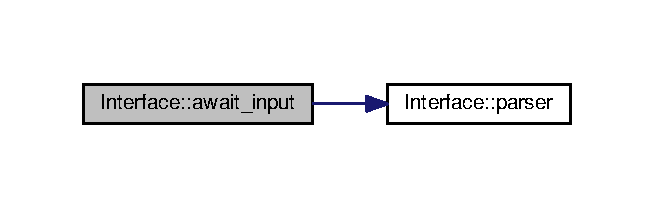
\includegraphics[width=350pt]{class_interface_a24b944dc66cb79f76ba91192a2a2860e_cgraph}
\end{center}
\end{figure}




Here is the caller graph for this function\+:\nopagebreak
\begin{figure}[H]
\begin{center}
\leavevmode
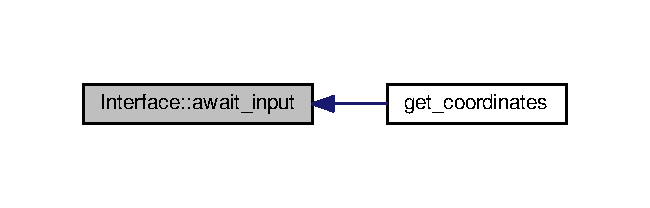
\includegraphics[width=350pt]{class_interface_a24b944dc66cb79f76ba91192a2a2860e_icgraph}
\end{center}
\end{figure}


\index{Interface@{Interface}!get\+\_\+specification@{get\+\_\+specification}}
\index{get\+\_\+specification@{get\+\_\+specification}!Interface@{Interface}}
\subsubsection[{\texorpdfstring{get\+\_\+specification() const }{get_specification() const }}]{\setlength{\rightskip}{0pt plus 5cm}uint8\+\_\+t Interface\+::get\+\_\+specification (
\begin{DoxyParamCaption}
{}
\end{DoxyParamCaption}
) const}\hypertarget{class_interface_adfa71e85801e5bb0e8bc88da902f8133}{}\label{class_interface_adfa71e85801e5bb0e8bc88da902f8133}


getter for the specification. 

\begin{DoxyReturn}{Returns}
specification pair filled with shape and colour 
\end{DoxyReturn}


Definition at line 111 of file interface.\+cpp.



Here is the caller graph for this function\+:\nopagebreak
\begin{figure}[H]
\begin{center}
\leavevmode
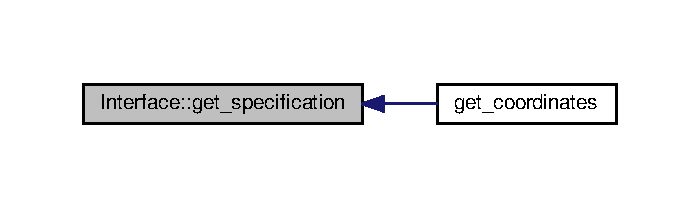
\includegraphics[width=350pt]{class_interface_adfa71e85801e5bb0e8bc88da902f8133_icgraph}
\end{center}
\end{figure}


\index{Interface@{Interface}!input@{input}}
\index{input@{input}!Interface@{Interface}}
\subsubsection[{\texorpdfstring{input()}{input()}}]{\setlength{\rightskip}{0pt plus 5cm}string Interface\+::input (
\begin{DoxyParamCaption}
{}
\end{DoxyParamCaption}
)\hspace{0.3cm}{\ttfamily [private]}}\hypertarget{class_interface_ab6e3210b017ae87be6ecf3b0fdd29d89}{}\label{class_interface_ab6e3210b017ae87be6ecf3b0fdd29d89}


Function to wait and extract input data from user through the console. 

\begin{DoxyReturn}{Returns}
string of input characters 
\end{DoxyReturn}


Definition at line 20 of file interface.\+cpp.



Here is the caller graph for this function\+:\nopagebreak
\begin{figure}[H]
\begin{center}
\leavevmode
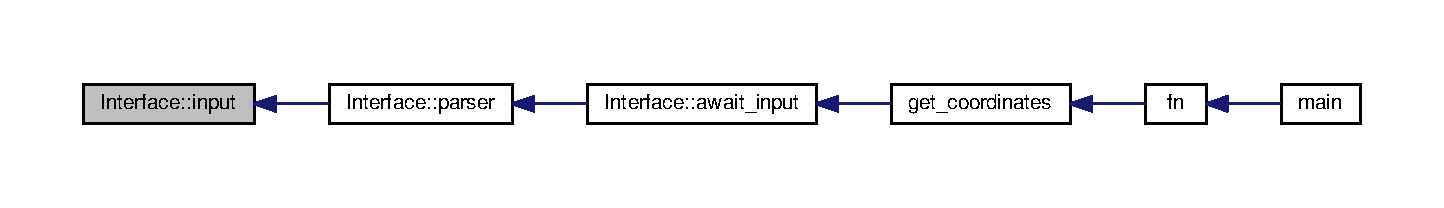
\includegraphics[width=350pt]{class_interface_ab6e3210b017ae87be6ecf3b0fdd29d89_icgraph}
\end{center}
\end{figure}


\index{Interface@{Interface}!parser@{parser}}
\index{parser@{parser}!Interface@{Interface}}
\subsubsection[{\texorpdfstring{parser(bool first\+\_\+time)}{parser(bool first_time)}}]{\setlength{\rightskip}{0pt plus 5cm}int8\+\_\+t Interface\+::parser (
\begin{DoxyParamCaption}
\item[{bool}]{first\+\_\+time}
\end{DoxyParamCaption}
)}\hypertarget{class_interface_a345faa7570aa36a31681ca850d1c283d}{}\label{class_interface_a345faa7570aa36a31681ca850d1c283d}


Function that will read the input and will then check if it is correct and translate the input to a pair filled with the choices of the user. It calls. 

\begin{DoxySeeAlso}{See also}
\hyperlink{class_interface_ab6e3210b017ae87be6ecf3b0fdd29d89}{input()} first to get the \hyperlink{class_interface_ab6e3210b017ae87be6ecf3b0fdd29d89}{input} from the user. This is not passed to the function. When \textquotesingle{}e\textquotesingle{} is put in, it will return 1 It supports a batch mode and accepts a line from a file. 

\hyperlink{class_interface_ab6e3210b017ae87be6ecf3b0fdd29d89}{input()} 
\end{DoxySeeAlso}

\begin{DoxyParams}{Parameters}
{\em line} & string with the read line \\
\hline
{\em batch} & parameter to set batch mode \\
\hline
\end{DoxyParams}
\begin{DoxyReturn}{Returns}
handling code 
\end{DoxyReturn}


Definition at line 28 of file interface.\+cpp.



Here is the call graph for this function\+:\nopagebreak
\begin{figure}[H]
\begin{center}
\leavevmode
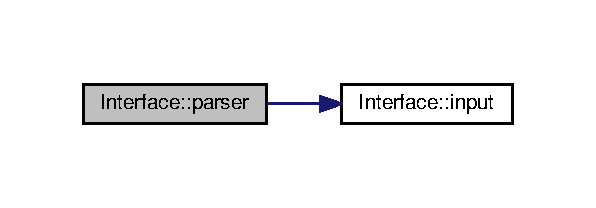
\includegraphics[width=286pt]{class_interface_a345faa7570aa36a31681ca850d1c283d_cgraph}
\end{center}
\end{figure}




Here is the caller graph for this function\+:\nopagebreak
\begin{figure}[H]
\begin{center}
\leavevmode
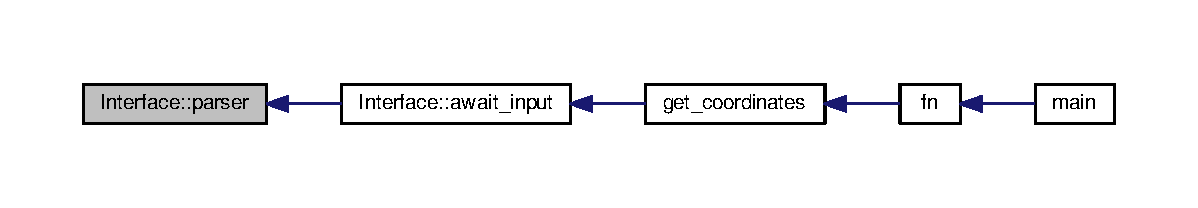
\includegraphics[width=350pt]{class_interface_a345faa7570aa36a31681ca850d1c283d_icgraph}
\end{center}
\end{figure}




\subsection{Member Data Documentation}
\index{Interface@{Interface}!specification@{specification}}
\index{specification@{specification}!Interface@{Interface}}
\subsubsection[{\texorpdfstring{specification}{specification}}]{\setlength{\rightskip}{0pt plus 5cm}uint8\+\_\+t Interface\+::specification\hspace{0.3cm}{\ttfamily [private]}}\hypertarget{class_interface_a8a5e47e57ef555ebbf54f345686e34cf}{}\label{class_interface_a8a5e47e57ef555ebbf54f345686e34cf}


Pair contains info about the chosen shape (first value) and the colour (second value). 



Definition at line 70 of file interface.\+hpp.



The documentation for this class was generated from the following files\+:\begin{DoxyCompactItemize}
\item 
src/\hyperlink{interface_8hpp}{interface.\+hpp}\item 
src/\hyperlink{interface_8cpp}{interface.\+cpp}\end{DoxyCompactItemize}

\hypertarget{class_matrix}{}\section{Matrix$<$ W, H, T $>$ Class Template Reference}
\label{class_matrix}\index{Matrix$<$ W, H, T $>$@{Matrix$<$ W, H, T $>$}}


{\ttfamily \#include $<$Matrix.\+hpp$>$}

\subsection*{Public Member Functions}
\begin{DoxyCompactItemize}
\item 
\hyperlink{class_matrix_a26e9ec6ddcde3891596c76e8fd753d04}{Matrix} (T default\+Value=0)
\item 
\hyperlink{class_matrix_a304fa7436faff40983551ed2d93b8583}{Matrix} (const std\+::initializer\+\_\+list$<$ T $>$ \&list)
\item 
\hyperlink{class_matrix_a266627bf345d07baa56e78c25013a83d}{Matrix} (const std\+::initializer\+\_\+list$<$ std\+::initializer\+\_\+list$<$ T $>$$>$ \&list)
\item 
\hyperlink{class_matrix_a94c464f26c4f31ff40674a2432ed9c6e}{Matrix} (const std\+::array$<$ std\+::array$<$ T, W $>$, H $>$ \&array)
\item 
\hyperlink{class_matrix_ad8895ac9cc7fc537addf48c1fb9497b9}{Matrix} (const \hyperlink{class_matrix}{Matrix}$<$ W, H, T $>$ \&other)
\item 
std\+::array$<$ T, W $>$ \hyperlink{class_matrix_ab33ffea8cb7e14c82d7ac183a9929198}{at} (std\+::size\+\_\+t height) const 
\item 
T \hyperlink{class_matrix_a9454a436ff7c18983b832642cc58b3ff}{at} (std\+::size\+\_\+t height, std\+::size\+\_\+t width) const 
\item 
std\+::array$<$ T, W $>$ \& \hyperlink{class_matrix_a5c110971f6c4b6282b937d0e815ab731}{operator\mbox{[}$\,$\mbox{]}} (const std\+::size\+\_\+t idx)
\item 
const \hyperlink{class_matrix}{Matrix}$<$ W, H, T $>$ \& \hyperlink{class_matrix_a20c1001ca220100453e36b15279b6ab7}{operator=} (const \hyperlink{class_matrix}{Matrix}$<$ W, H, T $>$ \&other)
\item 
{\footnotesize template$<$std\+::size\+\_\+t a\+Width, std\+::size\+\_\+t a\+Height, class aT $>$ }\\const \hyperlink{class_matrix}{Matrix} \hyperlink{class_matrix_a1b74e614af59905c38d68eb0daaffec7}{operator=} (const \hyperlink{class_matrix}{Matrix}$<$ a\+Width, a\+Height, aT $>$ \&other)
\item 
{\footnotesize template$<$std\+::size\+\_\+t a\+Width, std\+::size\+\_\+t a\+Height, class aT $>$ }\\bool \hyperlink{class_matrix_acb58c98e1e74826d92aee856ffc4a3b4}{operator==} (const \hyperlink{class_matrix}{Matrix}$<$ a\+Width, a\+Height, aT $>$ \&other)
\item 
std\+::size\+\_\+t \hyperlink{class_matrix_a7bc543fe8c5920f92aab8a172d963e8c}{size} () const 
\item 
std\+::size\+\_\+t \hyperlink{class_matrix_a9259f00c0dc87ef47a0823e4d5ebb429}{get\+Width} () const 
\item 
std\+::size\+\_\+t \hyperlink{class_matrix_a67a8079db706e47b4c59b5515bde766a}{get\+Height} () const 
\item 
\hyperlink{class_matrix}{Matrix}$<$ H, W, T $>$ \hyperlink{class_matrix_abb5e9bcfad1f5ed025294c599451c738}{transpose} () const 
\item 
\hyperlink{class_matrix}{Matrix}$<$ H, W, T $>$ \hyperlink{class_matrix_af079b7d71963122e484a1918351e5b16}{Invert} () const 
\item 
\hyperlink{class_matrix}{Matrix}$<$ W, H, T $>$ \hyperlink{class_matrix_aac7c89f565eca5c6a69bc721be2c7a63}{Swap} (unsigned long row1, unsigned long row2) const 
\item 
\hyperlink{class_matrix}{Matrix}$<$ W, H, T $>$ \hyperlink{class_matrix_aac2fa2441171eebbce6569cd085a9949}{Add} (unsigned long from, unsigned long to, double multiplier) const 
\item 
bool \hyperlink{class_matrix_a71d4fede301a6798bf5ea7df3abb0eaa}{appr} (const \hyperlink{class_matrix}{Matrix}$<$ W, H, T $>$ \&a, const \hyperlink{class_matrix}{Matrix}$<$ W, H, T $>$ \&b, double precision)
\item 
\hyperlink{class_matrix}{Matrix}$<$ W, H, T $>$ \hyperlink{class_matrix_a1cca7534031201f08afa146565310a98}{Identity} () const 
\item 
std\+::size\+\_\+t \hyperlink{class_matrix_a194c3692f1bbb0c80970fc5bae2b01a1}{get\+Highest\+Row} (const unsigned short i)
\item 
\hyperlink{class_matrix}{Matrix}$<$ H, W $\ast$2, T $>$ \hyperlink{class_matrix_adb725d9614aa45937766d87668e5e0cc}{h\+Concat} (const \hyperlink{class_matrix}{Matrix}$<$ H, W $\ast$2, T $>$ \&other) const 
\item 
{\footnotesize template$<$class aT  = T$>$ }\\\hyperlink{class_matrix}{Matrix}$<$ W, H, T $>$ \hyperlink{class_matrix_a47377a1da625f943895eec79daefa690}{point\+Wise\+Multiply} (const T value)
\item 
std\+::string \hyperlink{class_matrix_aa65e4a9c832a9134de9a2b4d0f7758df}{to\+\_\+string} () const 
\item 
\hyperlink{class_matrix}{Matrix}$<$ W, H, T $>$ \& \hyperlink{class_matrix_ad93704899e6667c756e06377d6e67d48}{operator$\ast$=} (const T \&scalar)
\item 
\hyperlink{class_matrix}{Matrix}$<$ W, H, T $>$ \hyperlink{class_matrix_ad1da3a066ba6d48c2f7952c6cc7b95d2}{operator$\ast$} (const T \&scalar) const 
\item 
{\footnotesize template$<$class aT  = T$>$ }\\\hyperlink{class_matrix}{Matrix}$<$ W, H, T $>$ \& \hyperlink{class_matrix_a162b1b5392a6c838baf43d4765027b3f}{operator/=} (const aT \&scalar)
\item 
{\footnotesize template$<$class aT  = T$>$ }\\\hyperlink{class_matrix}{Matrix}$<$ W, H, T $>$ \hyperlink{class_matrix_a0b62ff512870c79543e5d5e710e5e53b}{operator/} (const aT \&scalar) const 
\item 
\hyperlink{class_matrix}{Matrix}$<$ W, H, T $>$ \& \hyperlink{class_matrix_af1ce2eed120cde67df92e23a7f8b7b00}{operator+=} (const T \&value)
\item 
\hyperlink{class_matrix}{Matrix}$<$ W, H, T $>$ \hyperlink{class_matrix_af225dded660c20974f3a3c29b0360a8a}{operator+} (const T \&value)
\item 
{\footnotesize template$<$class aT  = T$>$ }\\\hyperlink{class_matrix}{Matrix}$<$ W, H, T $>$ \& \hyperlink{class_matrix_a1675e7e5ed541024cbc5fdc66114d23c}{operator-\/=} (const aT \&value)
\item 
{\footnotesize template$<$class aT  = T$>$ }\\\hyperlink{class_matrix}{Matrix}$<$ W, H, T $>$ \hyperlink{class_matrix_a1a3d0d98807ec9146bf0d1d374c10517}{operator-\/} (const aT \&value) const 
\item 
{\footnotesize template$<$std\+::size\+\_\+t a\+Width, std\+::size\+\_\+t a\+Height$>$ }\\\hyperlink{class_matrix}{Matrix}$<$ a\+Width, H, T $>$ \hyperlink{class_matrix_a7f339c5605cecdf38f2629ee54acdb4a}{operator$\ast$} (const \hyperlink{class_matrix}{Matrix}$<$ a\+Width, a\+Height, T $>$ \&other) const 
\item 
\hyperlink{class_matrix}{Matrix}$<$ W, H, T $>$ \& \hyperlink{class_matrix_a3fb20993c946d64ba102a4cc28f353f4}{operator+=} (const \hyperlink{class_matrix}{Matrix}$<$ W, H, T $>$ \&other)
\item 
\hyperlink{class_matrix}{Matrix}$<$ W, H, T $>$ \hyperlink{class_matrix_a5123d4078fb8145eb7c7dd4722b49845}{operator+} (const \hyperlink{class_matrix}{Matrix}$<$ W, H, T $>$ \&other)
\item 
\hyperlink{class_matrix}{Matrix}$<$ W, H, T $>$ \& \hyperlink{class_matrix_aae3a29e920db3256c1ccc3842ac0b15a}{operator-\/=} (const \hyperlink{class_matrix}{Matrix}$<$ W, H, T $>$ \&other)
\item 
\hyperlink{class_matrix}{Matrix}$<$ W, H, T $>$ \hyperlink{class_matrix_a2d80e2c5863a05d0917e9e5a02cc575b}{operator-\/} (\hyperlink{class_matrix}{Matrix}$<$ W, H, T $>$ \&other)
\item 
virtual \hyperlink{class_matrix_af9284a0f60b726bdb0e9a473d1e265f7}{$\sim$\+Matrix} ()
\item 
{\footnotesize template$<$std\+::size\+\_\+t a\+Width, std\+::size\+\_\+t a\+Height, class aT $>$ }\\const \hyperlink{class_matrix}{Matrix}$<$ W, H, T $>$ \hyperlink{class_matrix_a09e6b5e23cef709c63ce2ec0a0ccce2d}{operator=} (const \hyperlink{class_matrix}{Matrix}$<$ a\+Width, a\+Height, aT $>$ \&other)
\end{DoxyCompactItemize}


\subsection{Detailed Description}
\subsubsection*{template$<$std\+::size\+\_\+t W, std\+::size\+\_\+t H, class T = int$>$\\*
class Matrix$<$ W, H, T $>$}



Definition at line 18 of file Matrix.\+hpp.



\subsection{Constructor \& Destructor Documentation}
\index{Matrix@{Matrix}!Matrix@{Matrix}}
\index{Matrix@{Matrix}!Matrix@{Matrix}}
\subsubsection[{\texorpdfstring{Matrix(\+T default\+Value=0)}{Matrix(T defaultValue=0)}}]{\setlength{\rightskip}{0pt plus 5cm}template$<$std\+::size\+\_\+t W, std\+::size\+\_\+t H, class T $>$ {\bf Matrix}$<$ W, H, T $>$\+::{\bf Matrix} (
\begin{DoxyParamCaption}
\item[{T}]{default\+Value = {\ttfamily 0}}
\end{DoxyParamCaption}
)}\hypertarget{class_matrix_a26e9ec6ddcde3891596c76e8fd753d04}{}\label{class_matrix_a26e9ec6ddcde3891596c76e8fd753d04}


Definition at line 150 of file Matrix.\+hpp.

\index{Matrix@{Matrix}!Matrix@{Matrix}}
\index{Matrix@{Matrix}!Matrix@{Matrix}}
\subsubsection[{\texorpdfstring{Matrix(const std\+::initializer\+\_\+list$<$ T $>$ \&list)}{Matrix(const std::initializer_list< T > &list)}}]{\setlength{\rightskip}{0pt plus 5cm}template$<$std\+::size\+\_\+t W, std\+::size\+\_\+t H, class T $>$ {\bf Matrix}$<$ W, H, T $>$\+::{\bf Matrix} (
\begin{DoxyParamCaption}
\item[{const std\+::initializer\+\_\+list$<$ T $>$ \&}]{list}
\end{DoxyParamCaption}
)}\hypertarget{class_matrix_a304fa7436faff40983551ed2d93b8583}{}\label{class_matrix_a304fa7436faff40983551ed2d93b8583}


Definition at line 159 of file Matrix.\+hpp.

\index{Matrix@{Matrix}!Matrix@{Matrix}}
\index{Matrix@{Matrix}!Matrix@{Matrix}}
\subsubsection[{\texorpdfstring{Matrix(const std\+::initializer\+\_\+list$<$ std\+::initializer\+\_\+list$<$ T $>$$>$ \&list)}{Matrix(const std::initializer_list< std::initializer_list< T >> &list)}}]{\setlength{\rightskip}{0pt plus 5cm}template$<$std\+::size\+\_\+t W, std\+::size\+\_\+t H, class T $>$ {\bf Matrix}$<$ W, H, T $>$\+::{\bf Matrix} (
\begin{DoxyParamCaption}
\item[{const std\+::initializer\+\_\+list$<$ std\+::initializer\+\_\+list$<$ T $>$$>$ \&}]{list}
\end{DoxyParamCaption}
)}\hypertarget{class_matrix_a266627bf345d07baa56e78c25013a83d}{}\label{class_matrix_a266627bf345d07baa56e78c25013a83d}


Definition at line 181 of file Matrix.\+hpp.

\index{Matrix@{Matrix}!Matrix@{Matrix}}
\index{Matrix@{Matrix}!Matrix@{Matrix}}
\subsubsection[{\texorpdfstring{Matrix(const std\+::array$<$ std\+::array$<$ T, W $>$, H $>$ \&array)}{Matrix(const std::array< std::array< T, W >, H > &array)}}]{\setlength{\rightskip}{0pt plus 5cm}template$<$std\+::size\+\_\+t W, std\+::size\+\_\+t H, class T $>$ {\bf Matrix}$<$ W, H, T $>$\+::{\bf Matrix} (
\begin{DoxyParamCaption}
\item[{const std\+::array$<$ std\+::array$<$ T, W $>$, H $>$ \&}]{array}
\end{DoxyParamCaption}
)}\hypertarget{class_matrix_a94c464f26c4f31ff40674a2432ed9c6e}{}\label{class_matrix_a94c464f26c4f31ff40674a2432ed9c6e}


Definition at line 211 of file Matrix.\+hpp.

\index{Matrix@{Matrix}!Matrix@{Matrix}}
\index{Matrix@{Matrix}!Matrix@{Matrix}}
\subsubsection[{\texorpdfstring{Matrix(const Matrix$<$ W, H, T $>$ \&other)}{Matrix(const Matrix< W, H, T > &other)}}]{\setlength{\rightskip}{0pt plus 5cm}template$<$std\+::size\+\_\+t W, std\+::size\+\_\+t H, class T $>$ {\bf Matrix}$<$ W, H, T $>$\+::{\bf Matrix} (
\begin{DoxyParamCaption}
\item[{const {\bf Matrix}$<$ W, H, T $>$ \&}]{other}
\end{DoxyParamCaption}
)}\hypertarget{class_matrix_ad8895ac9cc7fc537addf48c1fb9497b9}{}\label{class_matrix_ad8895ac9cc7fc537addf48c1fb9497b9}


Definition at line 218 of file Matrix.\+hpp.

\index{Matrix@{Matrix}!````~Matrix@{$\sim$\+Matrix}}
\index{````~Matrix@{$\sim$\+Matrix}!Matrix@{Matrix}}
\subsubsection[{\texorpdfstring{$\sim$\+Matrix()}{~Matrix()}}]{\setlength{\rightskip}{0pt plus 5cm}template$<$std\+::size\+\_\+t W, std\+::size\+\_\+t H, class T $>$ {\bf Matrix}$<$ W, H, T $>$\+::$\sim${\bf Matrix} (
\begin{DoxyParamCaption}
{}
\end{DoxyParamCaption}
)\hspace{0.3cm}{\ttfamily [virtual]}}\hypertarget{class_matrix_af9284a0f60b726bdb0e9a473d1e265f7}{}\label{class_matrix_af9284a0f60b726bdb0e9a473d1e265f7}


Definition at line 649 of file Matrix.\+hpp.



Here is the caller graph for this function\+:\nopagebreak
\begin{figure}[H]
\begin{center}
\leavevmode
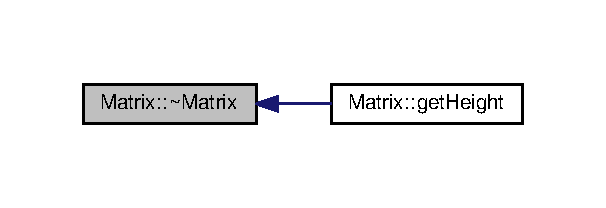
\includegraphics[width=291pt]{class_matrix_af9284a0f60b726bdb0e9a473d1e265f7_icgraph}
\end{center}
\end{figure}




\subsection{Member Function Documentation}
\index{Matrix@{Matrix}!Add@{Add}}
\index{Add@{Add}!Matrix@{Matrix}}
\subsubsection[{\texorpdfstring{Add(unsigned long from, unsigned long to, double multiplier) const }{Add(unsigned long from, unsigned long to, double multiplier) const }}]{\setlength{\rightskip}{0pt plus 5cm}template$<$std\+::size\+\_\+t W, std\+::size\+\_\+t H, class T $>$ {\bf Matrix}$<$ W, H, T $>$ {\bf Matrix}$<$ W, H, T $>$\+::Add (
\begin{DoxyParamCaption}
\item[{unsigned long}]{from, }
\item[{unsigned long}]{to, }
\item[{double}]{multiplier}
\end{DoxyParamCaption}
) const}\hypertarget{class_matrix_aac2fa2441171eebbce6569cd085a9949}{}\label{class_matrix_aac2fa2441171eebbce6569cd085a9949}


Definition at line 340 of file Matrix.\+hpp.



Here is the caller graph for this function\+:\nopagebreak
\begin{figure}[H]
\begin{center}
\leavevmode
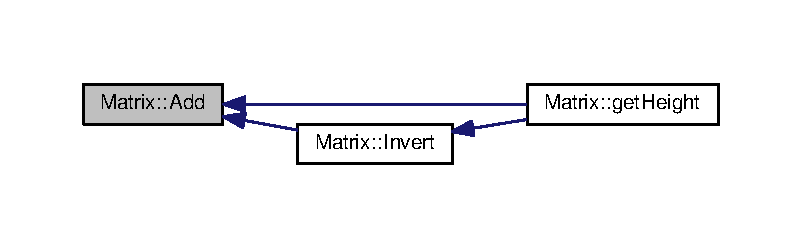
\includegraphics[width=350pt]{class_matrix_aac2fa2441171eebbce6569cd085a9949_icgraph}
\end{center}
\end{figure}


\index{Matrix@{Matrix}!appr@{appr}}
\index{appr@{appr}!Matrix@{Matrix}}
\subsubsection[{\texorpdfstring{appr(const Matrix$<$ W, H, T $>$ \&a, const Matrix$<$ W, H, T $>$ \&b, double precision)}{appr(const Matrix< W, H, T > &a, const Matrix< W, H, T > &b, double precision)}}]{\setlength{\rightskip}{0pt plus 5cm}template$<$std\+::size\+\_\+t W, std\+::size\+\_\+t H, class T $>$ bool {\bf Matrix}$<$ W, H, T $>$\+::appr (
\begin{DoxyParamCaption}
\item[{const {\bf Matrix}$<$ W, H, T $>$ \&}]{a, }
\item[{const {\bf Matrix}$<$ W, H, T $>$ \&}]{b, }
\item[{double}]{precision}
\end{DoxyParamCaption}
)}\hypertarget{class_matrix_a71d4fede301a6798bf5ea7df3abb0eaa}{}\label{class_matrix_a71d4fede301a6798bf5ea7df3abb0eaa}


Definition at line 355 of file Matrix.\+hpp.



Here is the call graph for this function\+:\nopagebreak
\begin{figure}[H]
\begin{center}
\leavevmode
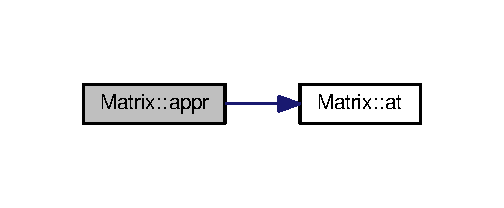
\includegraphics[width=242pt]{class_matrix_a71d4fede301a6798bf5ea7df3abb0eaa_cgraph}
\end{center}
\end{figure}




Here is the caller graph for this function\+:\nopagebreak
\begin{figure}[H]
\begin{center}
\leavevmode
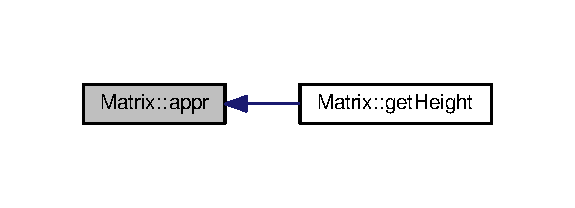
\includegraphics[width=276pt]{class_matrix_a71d4fede301a6798bf5ea7df3abb0eaa_icgraph}
\end{center}
\end{figure}


\index{Matrix@{Matrix}!at@{at}}
\index{at@{at}!Matrix@{Matrix}}
\subsubsection[{\texorpdfstring{at(std\+::size\+\_\+t height) const }{at(std::size_t height) const }}]{\setlength{\rightskip}{0pt plus 5cm}template$<$std\+::size\+\_\+t W, std\+::size\+\_\+t H, class T $>$ std\+::array$<$ T, W $>$ {\bf Matrix}$<$ W, H, T $>$\+::at (
\begin{DoxyParamCaption}
\item[{std\+::size\+\_\+t}]{height}
\end{DoxyParamCaption}
) const}\hypertarget{class_matrix_ab33ffea8cb7e14c82d7ac183a9929198}{}\label{class_matrix_ab33ffea8cb7e14c82d7ac183a9929198}


Definition at line 225 of file Matrix.\+hpp.



Here is the caller graph for this function\+:\nopagebreak
\begin{figure}[H]
\begin{center}
\leavevmode
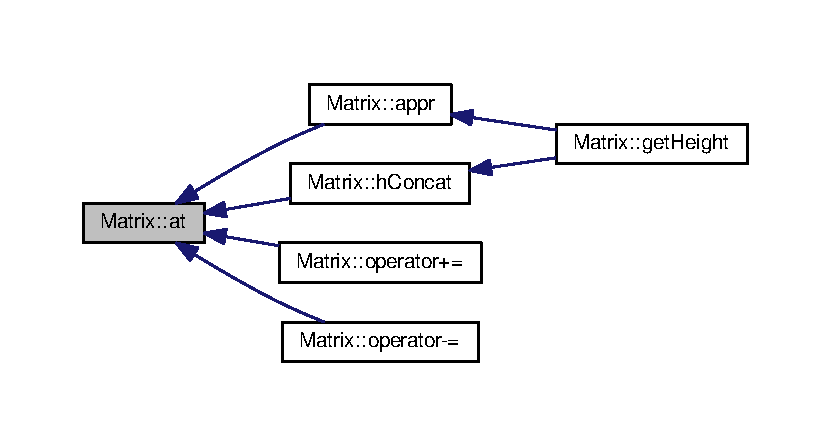
\includegraphics[width=350pt]{class_matrix_ab33ffea8cb7e14c82d7ac183a9929198_icgraph}
\end{center}
\end{figure}


\index{Matrix@{Matrix}!at@{at}}
\index{at@{at}!Matrix@{Matrix}}
\subsubsection[{\texorpdfstring{at(std\+::size\+\_\+t height, std\+::size\+\_\+t width) const }{at(std::size_t height, std::size_t width) const }}]{\setlength{\rightskip}{0pt plus 5cm}template$<$std\+::size\+\_\+t W, std\+::size\+\_\+t H, class T $>$ T {\bf Matrix}$<$ W, H, T $>$\+::at (
\begin{DoxyParamCaption}
\item[{std\+::size\+\_\+t}]{height, }
\item[{std\+::size\+\_\+t}]{width}
\end{DoxyParamCaption}
) const}\hypertarget{class_matrix_a9454a436ff7c18983b832642cc58b3ff}{}\label{class_matrix_a9454a436ff7c18983b832642cc58b3ff}


Definition at line 231 of file Matrix.\+hpp.

\index{Matrix@{Matrix}!get\+Height@{get\+Height}}
\index{get\+Height@{get\+Height}!Matrix@{Matrix}}
\subsubsection[{\texorpdfstring{get\+Height() const }{getHeight() const }}]{\setlength{\rightskip}{0pt plus 5cm}template$<$std\+::size\+\_\+t W, std\+::size\+\_\+t H, class T = int$>$ std\+::size\+\_\+t {\bf Matrix}$<$ W, H, T $>$\+::get\+Height (
\begin{DoxyParamCaption}
{}
\end{DoxyParamCaption}
) const\hspace{0.3cm}{\ttfamily [inline]}}\hypertarget{class_matrix_a67a8079db706e47b4c59b5515bde766a}{}\label{class_matrix_a67a8079db706e47b4c59b5515bde766a}


Definition at line 67 of file Matrix.\+hpp.



Here is the call graph for this function\+:\nopagebreak
\begin{figure}[H]
\begin{center}
\leavevmode
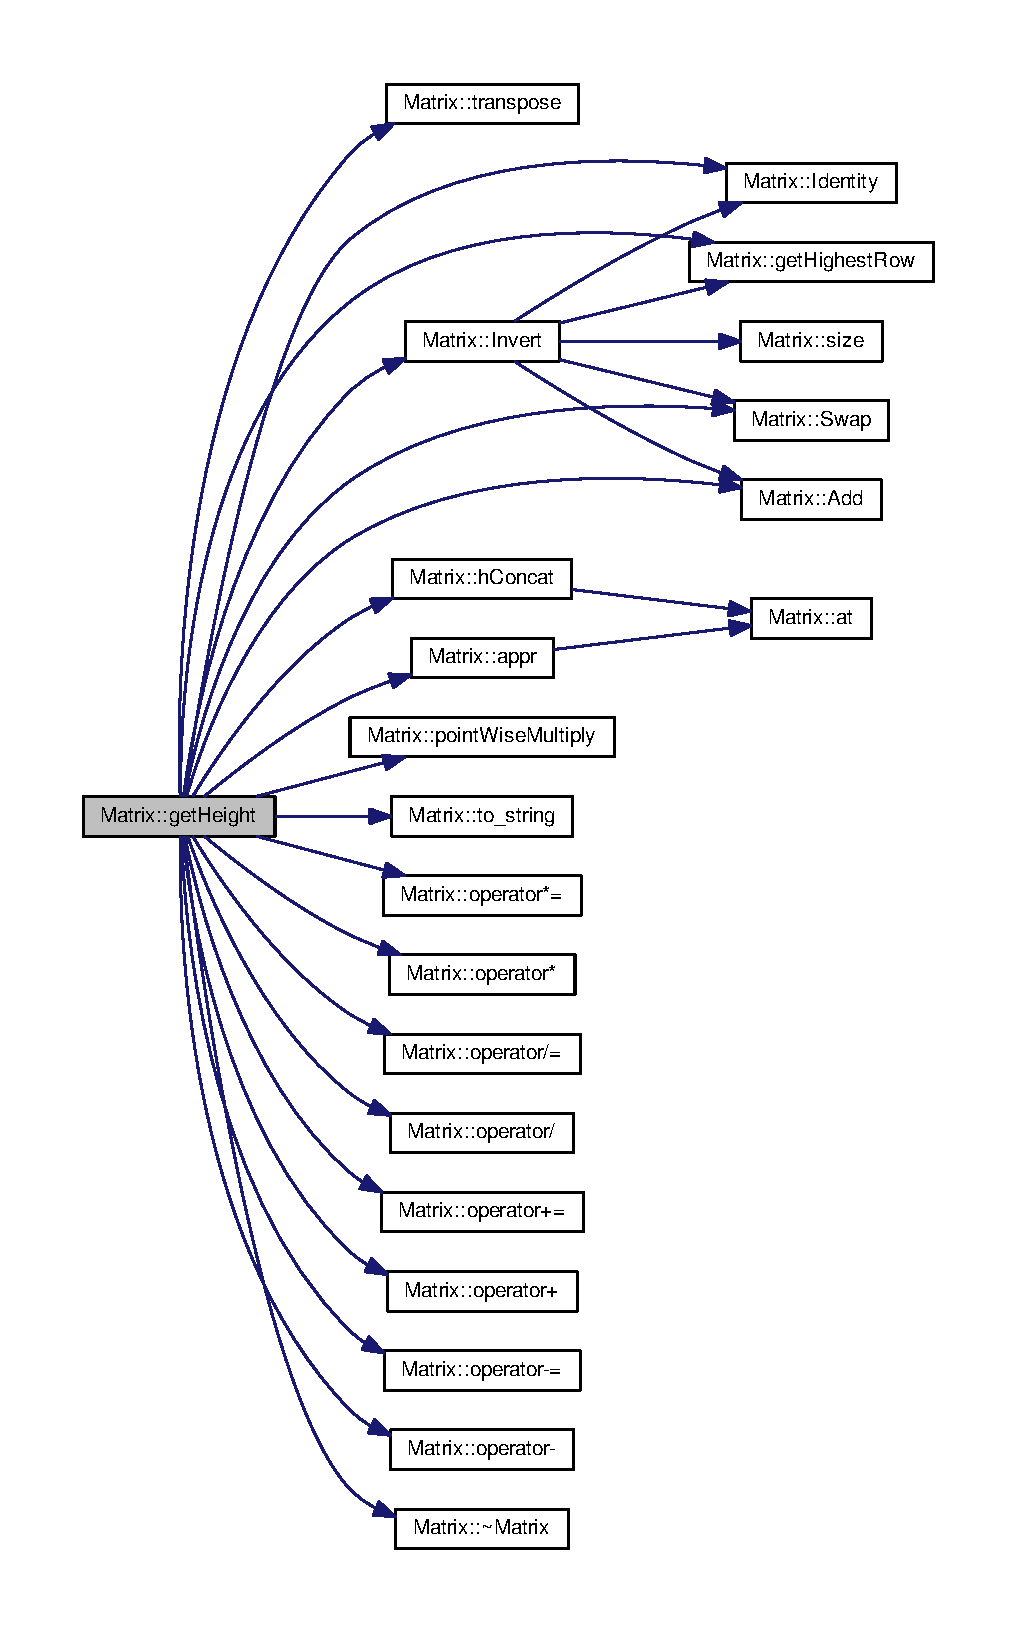
\includegraphics[height=550pt]{class_matrix_a67a8079db706e47b4c59b5515bde766a_cgraph}
\end{center}
\end{figure}


\index{Matrix@{Matrix}!get\+Highest\+Row@{get\+Highest\+Row}}
\index{get\+Highest\+Row@{get\+Highest\+Row}!Matrix@{Matrix}}
\subsubsection[{\texorpdfstring{get\+Highest\+Row(const unsigned short i)}{getHighestRow(const unsigned short i)}}]{\setlength{\rightskip}{0pt plus 5cm}template$<$std\+::size\+\_\+t W, std\+::size\+\_\+t H, class T $>$ std\+::size\+\_\+t {\bf Matrix}$<$ W, H, T $>$\+::get\+Highest\+Row (
\begin{DoxyParamCaption}
\item[{const unsigned short}]{i}
\end{DoxyParamCaption}
)}\hypertarget{class_matrix_a194c3692f1bbb0c80970fc5bae2b01a1}{}\label{class_matrix_a194c3692f1bbb0c80970fc5bae2b01a1}


Definition at line 380 of file Matrix.\+hpp.



Here is the caller graph for this function\+:\nopagebreak
\begin{figure}[H]
\begin{center}
\leavevmode
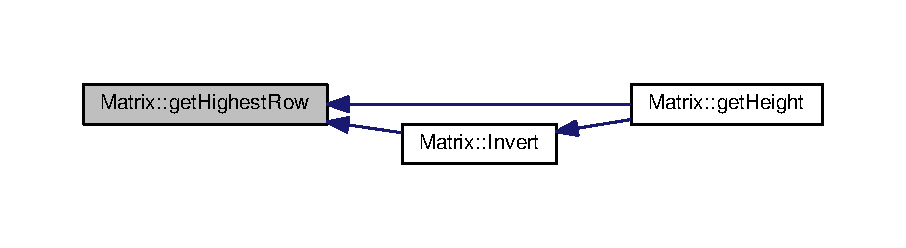
\includegraphics[width=350pt]{class_matrix_a194c3692f1bbb0c80970fc5bae2b01a1_icgraph}
\end{center}
\end{figure}


\index{Matrix@{Matrix}!get\+Width@{get\+Width}}
\index{get\+Width@{get\+Width}!Matrix@{Matrix}}
\subsubsection[{\texorpdfstring{get\+Width() const }{getWidth() const }}]{\setlength{\rightskip}{0pt plus 5cm}template$<$std\+::size\+\_\+t W, std\+::size\+\_\+t H, class T = int$>$ std\+::size\+\_\+t {\bf Matrix}$<$ W, H, T $>$\+::get\+Width (
\begin{DoxyParamCaption}
{}
\end{DoxyParamCaption}
) const\hspace{0.3cm}{\ttfamily [inline]}}\hypertarget{class_matrix_a9259f00c0dc87ef47a0823e4d5ebb429}{}\label{class_matrix_a9259f00c0dc87ef47a0823e4d5ebb429}


Definition at line 62 of file Matrix.\+hpp.

\index{Matrix@{Matrix}!h\+Concat@{h\+Concat}}
\index{h\+Concat@{h\+Concat}!Matrix@{Matrix}}
\subsubsection[{\texorpdfstring{h\+Concat(const Matrix$<$ H, W $\ast$2, T $>$ \&other) const }{hConcat(const Matrix< H, W *2, T > &other) const }}]{\setlength{\rightskip}{0pt plus 5cm}template$<$std\+::size\+\_\+t W, std\+::size\+\_\+t H, class T $>$ {\bf Matrix}$<$ H, W $\ast$2, T $>$ {\bf Matrix}$<$ W, H, T $>$\+::h\+Concat (
\begin{DoxyParamCaption}
\item[{const {\bf Matrix}$<$ H, W $\ast$2, T $>$ \&}]{other}
\end{DoxyParamCaption}
) const}\hypertarget{class_matrix_adb725d9614aa45937766d87668e5e0cc}{}\label{class_matrix_adb725d9614aa45937766d87668e5e0cc}


Definition at line 407 of file Matrix.\+hpp.



Here is the call graph for this function\+:\nopagebreak
\begin{figure}[H]
\begin{center}
\leavevmode
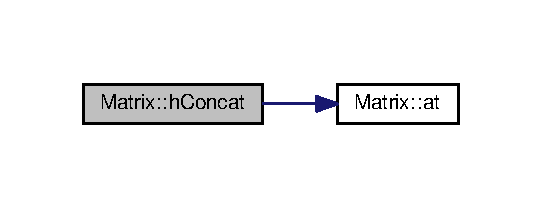
\includegraphics[width=260pt]{class_matrix_adb725d9614aa45937766d87668e5e0cc_cgraph}
\end{center}
\end{figure}




Here is the caller graph for this function\+:\nopagebreak
\begin{figure}[H]
\begin{center}
\leavevmode
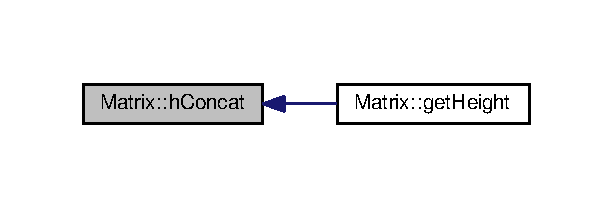
\includegraphics[width=294pt]{class_matrix_adb725d9614aa45937766d87668e5e0cc_icgraph}
\end{center}
\end{figure}


\index{Matrix@{Matrix}!Identity@{Identity}}
\index{Identity@{Identity}!Matrix@{Matrix}}
\subsubsection[{\texorpdfstring{Identity() const }{Identity() const }}]{\setlength{\rightskip}{0pt plus 5cm}template$<$std\+::size\+\_\+t W, std\+::size\+\_\+t H, class T $>$ {\bf Matrix}$<$ W, H, T $>$ {\bf Matrix}$<$ W, H, T $>$\+::Identity (
\begin{DoxyParamCaption}
{}
\end{DoxyParamCaption}
) const}\hypertarget{class_matrix_a1cca7534031201f08afa146565310a98}{}\label{class_matrix_a1cca7534031201f08afa146565310a98}


Definition at line 366 of file Matrix.\+hpp.



Here is the caller graph for this function\+:\nopagebreak
\begin{figure}[H]
\begin{center}
\leavevmode
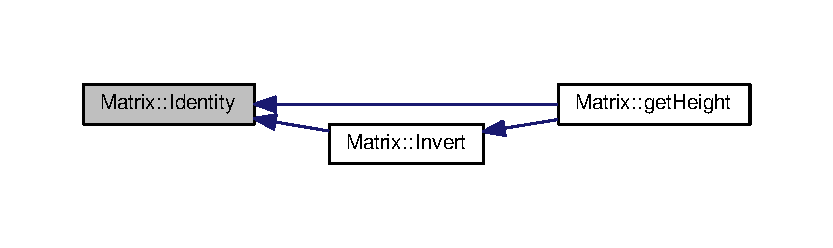
\includegraphics[width=350pt]{class_matrix_a1cca7534031201f08afa146565310a98_icgraph}
\end{center}
\end{figure}


\index{Matrix@{Matrix}!Invert@{Invert}}
\index{Invert@{Invert}!Matrix@{Matrix}}
\subsubsection[{\texorpdfstring{Invert() const }{Invert() const }}]{\setlength{\rightskip}{0pt plus 5cm}template$<$std\+::size\+\_\+t W, std\+::size\+\_\+t H, class T $>$ {\bf Matrix}$<$ H, W, T $>$ {\bf Matrix}$<$ W, H, T $>$\+::Invert (
\begin{DoxyParamCaption}
{}
\end{DoxyParamCaption}
) const}\hypertarget{class_matrix_af079b7d71963122e484a1918351e5b16}{}\label{class_matrix_af079b7d71963122e484a1918351e5b16}


Definition at line 424 of file Matrix.\+hpp.



Here is the call graph for this function\+:\nopagebreak
\begin{figure}[H]
\begin{center}
\leavevmode
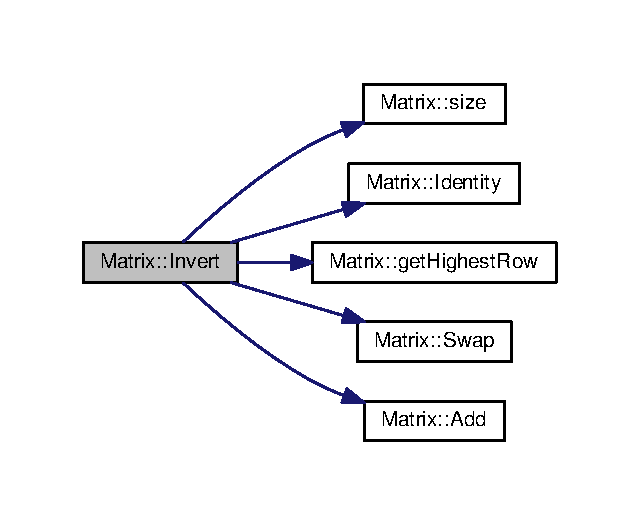
\includegraphics[width=307pt]{class_matrix_af079b7d71963122e484a1918351e5b16_cgraph}
\end{center}
\end{figure}




Here is the caller graph for this function\+:\nopagebreak
\begin{figure}[H]
\begin{center}
\leavevmode
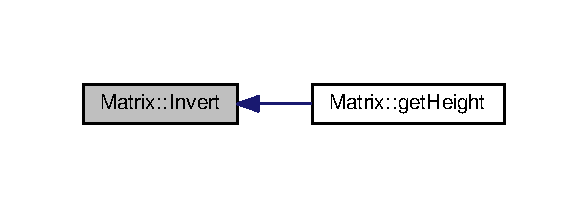
\includegraphics[width=282pt]{class_matrix_af079b7d71963122e484a1918351e5b16_icgraph}
\end{center}
\end{figure}


\index{Matrix@{Matrix}!operator$\ast$@{operator$\ast$}}
\index{operator$\ast$@{operator$\ast$}!Matrix@{Matrix}}
\subsubsection[{\texorpdfstring{operator$\ast$(const T \&scalar) const }{operator*(const T &scalar) const }}]{\setlength{\rightskip}{0pt plus 5cm}template$<$std\+::size\+\_\+t W, std\+::size\+\_\+t H, class T $>$ {\bf Matrix}$<$ W, H, T $>$ {\bf Matrix}$<$ W, H, T $>$\+::operator$\ast$ (
\begin{DoxyParamCaption}
\item[{const T \&}]{scalar}
\end{DoxyParamCaption}
) const}\hypertarget{class_matrix_ad1da3a066ba6d48c2f7952c6cc7b95d2}{}\label{class_matrix_ad1da3a066ba6d48c2f7952c6cc7b95d2}


Definition at line 511 of file Matrix.\+hpp.



Here is the caller graph for this function\+:\nopagebreak
\begin{figure}[H]
\begin{center}
\leavevmode
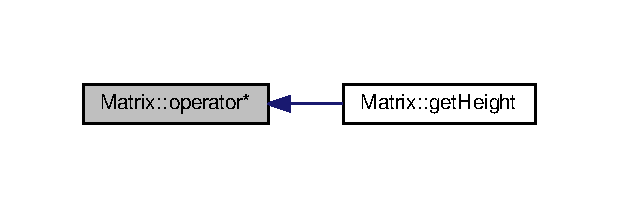
\includegraphics[width=297pt]{class_matrix_ad1da3a066ba6d48c2f7952c6cc7b95d2_icgraph}
\end{center}
\end{figure}


\index{Matrix@{Matrix}!operator$\ast$@{operator$\ast$}}
\index{operator$\ast$@{operator$\ast$}!Matrix@{Matrix}}
\subsubsection[{\texorpdfstring{operator$\ast$(const Matrix$<$ a\+Width, a\+Height, T $>$ \&other) const }{operator*(const Matrix< aWidth, aHeight, T > &other) const }}]{\setlength{\rightskip}{0pt plus 5cm}template$<$std\+::size\+\_\+t W, std\+::size\+\_\+t H, class T $>$ template$<$std\+::size\+\_\+t a\+Width, std\+::size\+\_\+t a\+Height$>$ {\bf Matrix}$<$ a\+Width, H, T $>$ {\bf Matrix}$<$ W, H, T $>$\+::operator$\ast$ (
\begin{DoxyParamCaption}
\item[{const {\bf Matrix}$<$ a\+Width, a\+Height, T $>$ \&}]{other}
\end{DoxyParamCaption}
) const}\hypertarget{class_matrix_a7f339c5605cecdf38f2629ee54acdb4a}{}\label{class_matrix_a7f339c5605cecdf38f2629ee54acdb4a}


Definition at line 583 of file Matrix.\+hpp.

\index{Matrix@{Matrix}!operator$\ast$=@{operator$\ast$=}}
\index{operator$\ast$=@{operator$\ast$=}!Matrix@{Matrix}}
\subsubsection[{\texorpdfstring{operator$\ast$=(const T \&scalar)}{operator*=(const T &scalar)}}]{\setlength{\rightskip}{0pt plus 5cm}template$<$std\+::size\+\_\+t W, std\+::size\+\_\+t H, class T $>$ {\bf Matrix}$<$ W, H, T $>$ \& {\bf Matrix}$<$ W, H, T $>$\+::operator$\ast$= (
\begin{DoxyParamCaption}
\item[{const T \&}]{scalar}
\end{DoxyParamCaption}
)}\hypertarget{class_matrix_ad93704899e6667c756e06377d6e67d48}{}\label{class_matrix_ad93704899e6667c756e06377d6e67d48}


Definition at line 498 of file Matrix.\+hpp.



Here is the caller graph for this function\+:\nopagebreak
\begin{figure}[H]
\begin{center}
\leavevmode
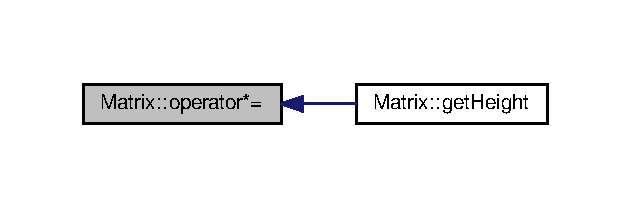
\includegraphics[width=303pt]{class_matrix_ad93704899e6667c756e06377d6e67d48_icgraph}
\end{center}
\end{figure}


\index{Matrix@{Matrix}!operator+@{operator+}}
\index{operator+@{operator+}!Matrix@{Matrix}}
\subsubsection[{\texorpdfstring{operator+(const T \&value)}{operator+(const T &value)}}]{\setlength{\rightskip}{0pt plus 5cm}template$<$std\+::size\+\_\+t W, std\+::size\+\_\+t H, class T $>$ {\bf Matrix}$<$ W, H, T $>$ {\bf Matrix}$<$ W, H, T $>$\+::operator+ (
\begin{DoxyParamCaption}
\item[{const T \&}]{value}
\end{DoxyParamCaption}
)}\hypertarget{class_matrix_af225dded660c20974f3a3c29b0360a8a}{}\label{class_matrix_af225dded660c20974f3a3c29b0360a8a}


Definition at line 553 of file Matrix.\+hpp.



Here is the caller graph for this function\+:\nopagebreak
\begin{figure}[H]
\begin{center}
\leavevmode
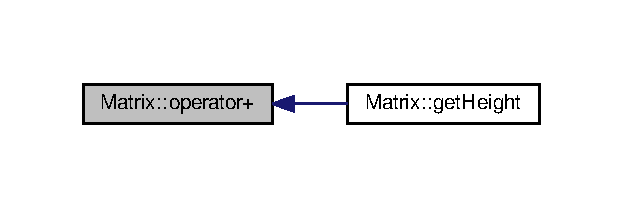
\includegraphics[width=299pt]{class_matrix_af225dded660c20974f3a3c29b0360a8a_icgraph}
\end{center}
\end{figure}


\index{Matrix@{Matrix}!operator+@{operator+}}
\index{operator+@{operator+}!Matrix@{Matrix}}
\subsubsection[{\texorpdfstring{operator+(const Matrix$<$ W, H, T $>$ \&other)}{operator+(const Matrix< W, H, T > &other)}}]{\setlength{\rightskip}{0pt plus 5cm}template$<$std\+::size\+\_\+t W, std\+::size\+\_\+t H, class T $>$ {\bf Matrix}$<$ W, H, T $>$ {\bf Matrix}$<$ W, H, T $>$\+::operator+ (
\begin{DoxyParamCaption}
\item[{const {\bf Matrix}$<$ W, H, T $>$ \&}]{other}
\end{DoxyParamCaption}
)}\hypertarget{class_matrix_a5123d4078fb8145eb7c7dd4722b49845}{}\label{class_matrix_a5123d4078fb8145eb7c7dd4722b49845}


Definition at line 622 of file Matrix.\+hpp.

\index{Matrix@{Matrix}!operator+=@{operator+=}}
\index{operator+=@{operator+=}!Matrix@{Matrix}}
\subsubsection[{\texorpdfstring{operator+=(const T \&value)}{operator+=(const T &value)}}]{\setlength{\rightskip}{0pt plus 5cm}template$<$std\+::size\+\_\+t W, std\+::size\+\_\+t H, class T $>$ {\bf Matrix}$<$ W, H, T $>$ \& {\bf Matrix}$<$ W, H, T $>$\+::operator+= (
\begin{DoxyParamCaption}
\item[{const T \&}]{value}
\end{DoxyParamCaption}
)}\hypertarget{class_matrix_af1ce2eed120cde67df92e23a7f8b7b00}{}\label{class_matrix_af1ce2eed120cde67df92e23a7f8b7b00}


Definition at line 540 of file Matrix.\+hpp.



Here is the caller graph for this function\+:\nopagebreak
\begin{figure}[H]
\begin{center}
\leavevmode
\includegraphics[width=305pt]{class_matrix_af1ce2eed120cde67df92e23a7f8b7b00_icgraph}
\end{center}
\end{figure}


\index{Matrix@{Matrix}!operator+=@{operator+=}}
\index{operator+=@{operator+=}!Matrix@{Matrix}}
\subsubsection[{\texorpdfstring{operator+=(const Matrix$<$ W, H, T $>$ \&other)}{operator+=(const Matrix< W, H, T > &other)}}]{\setlength{\rightskip}{0pt plus 5cm}template$<$std\+::size\+\_\+t W, std\+::size\+\_\+t H, class T $>$ {\bf Matrix}$<$ W, H, T $>$ \& {\bf Matrix}$<$ W, H, T $>$\+::operator+= (
\begin{DoxyParamCaption}
\item[{const {\bf Matrix}$<$ W, H, T $>$ \&}]{other}
\end{DoxyParamCaption}
)}\hypertarget{class_matrix_a3fb20993c946d64ba102a4cc28f353f4}{}\label{class_matrix_a3fb20993c946d64ba102a4cc28f353f4}


Definition at line 609 of file Matrix.\+hpp.



Here is the call graph for this function\+:\nopagebreak
\begin{figure}[H]
\begin{center}
\leavevmode
\includegraphics[width=271pt]{class_matrix_a3fb20993c946d64ba102a4cc28f353f4_cgraph}
\end{center}
\end{figure}


\index{Matrix@{Matrix}!operator-\/@{operator-\/}}
\index{operator-\/@{operator-\/}!Matrix@{Matrix}}
\subsubsection[{\texorpdfstring{operator-\/(const a\+T \&value) const }{operator-(const aT &value) const }}]{\setlength{\rightskip}{0pt plus 5cm}template$<$std\+::size\+\_\+t W, std\+::size\+\_\+t H, class T $>$ template$<$class aT $>$ {\bf Matrix}$<$ W, H, T $>$ {\bf Matrix}$<$ W, H, T $>$\+::operator-\/ (
\begin{DoxyParamCaption}
\item[{const aT \&}]{value}
\end{DoxyParamCaption}
) const}\hypertarget{class_matrix_a1a3d0d98807ec9146bf0d1d374c10517}{}\label{class_matrix_a1a3d0d98807ec9146bf0d1d374c10517}


Definition at line 575 of file Matrix.\+hpp.



Here is the caller graph for this function\+:\nopagebreak
\begin{figure}[H]
\begin{center}
\leavevmode
\includegraphics[width=296pt]{class_matrix_a1a3d0d98807ec9146bf0d1d374c10517_icgraph}
\end{center}
\end{figure}


\index{Matrix@{Matrix}!operator-\/@{operator-\/}}
\index{operator-\/@{operator-\/}!Matrix@{Matrix}}
\subsubsection[{\texorpdfstring{operator-\/(\+Matrix$<$ W, H, T $>$ \&other)}{operator-(Matrix< W, H, T > &other)}}]{\setlength{\rightskip}{0pt plus 5cm}template$<$std\+::size\+\_\+t W, std\+::size\+\_\+t H, class T $>$ {\bf Matrix}$<$ W, H, T $>$ {\bf Matrix}$<$ W, H, T $>$\+::operator-\/ (
\begin{DoxyParamCaption}
\item[{{\bf Matrix}$<$ W, H, T $>$ \&}]{other}
\end{DoxyParamCaption}
)}\hypertarget{class_matrix_a2d80e2c5863a05d0917e9e5a02cc575b}{}\label{class_matrix_a2d80e2c5863a05d0917e9e5a02cc575b}


Definition at line 642 of file Matrix.\+hpp.

\index{Matrix@{Matrix}!operator-\/=@{operator-\/=}}
\index{operator-\/=@{operator-\/=}!Matrix@{Matrix}}
\subsubsection[{\texorpdfstring{operator-\/=(const a\+T \&value)}{operator-=(const aT &value)}}]{\setlength{\rightskip}{0pt plus 5cm}template$<$std\+::size\+\_\+t W, std\+::size\+\_\+t H, class T $>$ template$<$class aT $>$ {\bf Matrix}$<$ W, H, T $>$ \& {\bf Matrix}$<$ W, H, T $>$\+::operator-\/= (
\begin{DoxyParamCaption}
\item[{const aT \&}]{value}
\end{DoxyParamCaption}
)}\hypertarget{class_matrix_a1675e7e5ed541024cbc5fdc66114d23c}{}\label{class_matrix_a1675e7e5ed541024cbc5fdc66114d23c}


Definition at line 561 of file Matrix.\+hpp.



Here is the caller graph for this function\+:\nopagebreak
\begin{figure}[H]
\begin{center}
\leavevmode
\includegraphics[width=302pt]{class_matrix_a1675e7e5ed541024cbc5fdc66114d23c_icgraph}
\end{center}
\end{figure}


\index{Matrix@{Matrix}!operator-\/=@{operator-\/=}}
\index{operator-\/=@{operator-\/=}!Matrix@{Matrix}}
\subsubsection[{\texorpdfstring{operator-\/=(const Matrix$<$ W, H, T $>$ \&other)}{operator-=(const Matrix< W, H, T > &other)}}]{\setlength{\rightskip}{0pt plus 5cm}template$<$std\+::size\+\_\+t W, std\+::size\+\_\+t H, class T $>$ {\bf Matrix}$<$ W, H, T $>$ \& {\bf Matrix}$<$ W, H, T $>$\+::operator-\/= (
\begin{DoxyParamCaption}
\item[{const {\bf Matrix}$<$ W, H, T $>$ \&}]{other}
\end{DoxyParamCaption}
)}\hypertarget{class_matrix_aae3a29e920db3256c1ccc3842ac0b15a}{}\label{class_matrix_aae3a29e920db3256c1ccc3842ac0b15a}


Definition at line 629 of file Matrix.\+hpp.



Here is the call graph for this function\+:\nopagebreak
\begin{figure}[H]
\begin{center}
\leavevmode
\includegraphics[width=268pt]{class_matrix_aae3a29e920db3256c1ccc3842ac0b15a_cgraph}
\end{center}
\end{figure}


\index{Matrix@{Matrix}!operator/@{operator/}}
\index{operator/@{operator/}!Matrix@{Matrix}}
\subsubsection[{\texorpdfstring{operator/(const a\+T \&scalar) const }{operator/(const aT &scalar) const }}]{\setlength{\rightskip}{0pt plus 5cm}template$<$std\+::size\+\_\+t W, std\+::size\+\_\+t H, class T $>$ template$<$class aT $>$ {\bf Matrix}$<$ W, H, T $>$ {\bf Matrix}$<$ W, H, T $>$\+::operator/ (
\begin{DoxyParamCaption}
\item[{const aT \&}]{scalar}
\end{DoxyParamCaption}
) const}\hypertarget{class_matrix_a0b62ff512870c79543e5d5e710e5e53b}{}\label{class_matrix_a0b62ff512870c79543e5d5e710e5e53b}


Definition at line 533 of file Matrix.\+hpp.



Here is the caller graph for this function\+:\nopagebreak
\begin{figure}[H]
\begin{center}
\leavevmode
\includegraphics[width=296pt]{class_matrix_a0b62ff512870c79543e5d5e710e5e53b_icgraph}
\end{center}
\end{figure}


\index{Matrix@{Matrix}!operator/=@{operator/=}}
\index{operator/=@{operator/=}!Matrix@{Matrix}}
\subsubsection[{\texorpdfstring{operator/=(const a\+T \&scalar)}{operator/=(const aT &scalar)}}]{\setlength{\rightskip}{0pt plus 5cm}template$<$std\+::size\+\_\+t W, std\+::size\+\_\+t H, class T $>$ template$<$class aT $>$ {\bf Matrix}$<$ W, H, T $>$ \& {\bf Matrix}$<$ W, H, T $>$\+::operator/= (
\begin{DoxyParamCaption}
\item[{const aT \&}]{scalar}
\end{DoxyParamCaption}
)}\hypertarget{class_matrix_a162b1b5392a6c838baf43d4765027b3f}{}\label{class_matrix_a162b1b5392a6c838baf43d4765027b3f}


Definition at line 519 of file Matrix.\+hpp.



Here is the caller graph for this function\+:\nopagebreak
\begin{figure}[H]
\begin{center}
\leavevmode
\includegraphics[width=302pt]{class_matrix_a162b1b5392a6c838baf43d4765027b3f_icgraph}
\end{center}
\end{figure}


\index{Matrix@{Matrix}!operator=@{operator=}}
\index{operator=@{operator=}!Matrix@{Matrix}}
\subsubsection[{\texorpdfstring{operator=(const Matrix$<$ W, H, T $>$ \&other)}{operator=(const Matrix< W, H, T > &other)}}]{\setlength{\rightskip}{0pt plus 5cm}template$<$std\+::size\+\_\+t W, std\+::size\+\_\+t H, class T $>$ const {\bf Matrix}$<$ W, H, T $>$ \& {\bf Matrix}$<$ W, H, T $>$\+::operator= (
\begin{DoxyParamCaption}
\item[{const {\bf Matrix}$<$ W, H, T $>$ \&}]{other}
\end{DoxyParamCaption}
)}\hypertarget{class_matrix_a20c1001ca220100453e36b15279b6ab7}{}\label{class_matrix_a20c1001ca220100453e36b15279b6ab7}


Definition at line 243 of file Matrix.\+hpp.

\index{Matrix@{Matrix}!operator=@{operator=}}
\index{operator=@{operator=}!Matrix@{Matrix}}
\subsubsection[{\texorpdfstring{operator=(const Matrix$<$ a\+Width, a\+Height, a\+T $>$ \&other)}{operator=(const Matrix< aWidth, aHeight, aT > &other)}}]{\setlength{\rightskip}{0pt plus 5cm}template$<$std\+::size\+\_\+t W, std\+::size\+\_\+t H, class T = int$>$ template$<$std\+::size\+\_\+t a\+Width, std\+::size\+\_\+t a\+Height, class aT $>$ const {\bf Matrix} {\bf Matrix}$<$ W, H, T $>$\+::operator= (
\begin{DoxyParamCaption}
\item[{const {\bf Matrix}$<$ a\+Width, a\+Height, aT $>$ \&}]{other}
\end{DoxyParamCaption}
)}\hypertarget{class_matrix_a1b74e614af59905c38d68eb0daaffec7}{}\label{class_matrix_a1b74e614af59905c38d68eb0daaffec7}
\index{Matrix@{Matrix}!operator=@{operator=}}
\index{operator=@{operator=}!Matrix@{Matrix}}
\subsubsection[{\texorpdfstring{operator=(const Matrix$<$ a\+Width, a\+Height, a\+T $>$ \&other)}{operator=(const Matrix< aWidth, aHeight, aT > &other)}}]{\setlength{\rightskip}{0pt plus 5cm}template$<$std\+::size\+\_\+t W, std\+::size\+\_\+t H, class T = int$>$ template$<$std\+::size\+\_\+t a\+Width, std\+::size\+\_\+t a\+Height, class aT $>$ const {\bf Matrix}$<$W, H, T$>$ {\bf Matrix}$<$ W, H, T $>$\+::operator= (
\begin{DoxyParamCaption}
\item[{const {\bf Matrix}$<$ a\+Width, a\+Height, aT $>$ \&}]{other}
\end{DoxyParamCaption}
)}\hypertarget{class_matrix_a09e6b5e23cef709c63ce2ec0a0ccce2d}{}\label{class_matrix_a09e6b5e23cef709c63ce2ec0a0ccce2d}


Definition at line 254 of file Matrix.\+hpp.

\index{Matrix@{Matrix}!operator==@{operator==}}
\index{operator==@{operator==}!Matrix@{Matrix}}
\subsubsection[{\texorpdfstring{operator==(const Matrix$<$ a\+Width, a\+Height, a\+T $>$ \&other)}{operator==(const Matrix< aWidth, aHeight, aT > &other)}}]{\setlength{\rightskip}{0pt plus 5cm}template$<$std\+::size\+\_\+t W, std\+::size\+\_\+t H, class T $>$ template$<$std\+::size\+\_\+t a\+Width, std\+::size\+\_\+t a\+Height, class aT $>$ bool {\bf Matrix}$<$ W, H, T $>$\+::operator== (
\begin{DoxyParamCaption}
\item[{const {\bf Matrix}$<$ a\+Width, a\+Height, aT $>$ \&}]{other}
\end{DoxyParamCaption}
)}\hypertarget{class_matrix_acb58c98e1e74826d92aee856ffc4a3b4}{}\label{class_matrix_acb58c98e1e74826d92aee856ffc4a3b4}


Definition at line 264 of file Matrix.\+hpp.

\index{Matrix@{Matrix}!operator\mbox{[}$\,$\mbox{]}@{operator[]}}
\index{operator\mbox{[}$\,$\mbox{]}@{operator[]}!Matrix@{Matrix}}
\subsubsection[{\texorpdfstring{operator[](const std\+::size\+\_\+t idx)}{operator[](const std::size_t idx)}}]{\setlength{\rightskip}{0pt plus 5cm}template$<$std\+::size\+\_\+t W, std\+::size\+\_\+t H, class T $>$ std\+::array$<$ T, W $>$ \& {\bf Matrix}$<$ W, H, T $>$\+::operator\mbox{[}$\,$\mbox{]} (
\begin{DoxyParamCaption}
\item[{const std\+::size\+\_\+t}]{idx}
\end{DoxyParamCaption}
)}\hypertarget{class_matrix_a5c110971f6c4b6282b937d0e815ab731}{}\label{class_matrix_a5c110971f6c4b6282b937d0e815ab731}


Definition at line 237 of file Matrix.\+hpp.

\index{Matrix@{Matrix}!point\+Wise\+Multiply@{point\+Wise\+Multiply}}
\index{point\+Wise\+Multiply@{point\+Wise\+Multiply}!Matrix@{Matrix}}
\subsubsection[{\texorpdfstring{point\+Wise\+Multiply(const T value)}{pointWiseMultiply(const T value)}}]{\setlength{\rightskip}{0pt plus 5cm}template$<$std\+::size\+\_\+t W, std\+::size\+\_\+t H, class T $>$ template$<$class aT $>$ {\bf Matrix}$<$ W, H, T $>$ {\bf Matrix}$<$ W, H, T $>$\+::point\+Wise\+Multiply (
\begin{DoxyParamCaption}
\item[{const T}]{value}
\end{DoxyParamCaption}
)}\hypertarget{class_matrix_a47377a1da625f943895eec79daefa690}{}\label{class_matrix_a47377a1da625f943895eec79daefa690}


Definition at line 297 of file Matrix.\+hpp.



Here is the caller graph for this function\+:\nopagebreak
\begin{figure}[H]
\begin{center}
\leavevmode
\includegraphics[width=335pt]{class_matrix_a47377a1da625f943895eec79daefa690_icgraph}
\end{center}
\end{figure}


\index{Matrix@{Matrix}!size@{size}}
\index{size@{size}!Matrix@{Matrix}}
\subsubsection[{\texorpdfstring{size() const }{size() const }}]{\setlength{\rightskip}{0pt plus 5cm}template$<$std\+::size\+\_\+t W, std\+::size\+\_\+t H, class T = int$>$ std\+::size\+\_\+t {\bf Matrix}$<$ W, H, T $>$\+::size (
\begin{DoxyParamCaption}
{}
\end{DoxyParamCaption}
) const\hspace{0.3cm}{\ttfamily [inline]}}\hypertarget{class_matrix_a7bc543fe8c5920f92aab8a172d963e8c}{}\label{class_matrix_a7bc543fe8c5920f92aab8a172d963e8c}


Definition at line 57 of file Matrix.\+hpp.



Here is the caller graph for this function\+:\nopagebreak
\begin{figure}[H]
\begin{center}
\leavevmode
\includegraphics[width=350pt]{class_matrix_a7bc543fe8c5920f92aab8a172d963e8c_icgraph}
\end{center}
\end{figure}


\index{Matrix@{Matrix}!Swap@{Swap}}
\index{Swap@{Swap}!Matrix@{Matrix}}
\subsubsection[{\texorpdfstring{Swap(unsigned long row1, unsigned long row2) const }{Swap(unsigned long row1, unsigned long row2) const }}]{\setlength{\rightskip}{0pt plus 5cm}template$<$std\+::size\+\_\+t W, std\+::size\+\_\+t H, class T $>$ {\bf Matrix}$<$ W, H, T $>$ {\bf Matrix}$<$ W, H, T $>$\+::Swap (
\begin{DoxyParamCaption}
\item[{unsigned long}]{row1, }
\item[{unsigned long}]{row2}
\end{DoxyParamCaption}
) const}\hypertarget{class_matrix_aac7c89f565eca5c6a69bc721be2c7a63}{}\label{class_matrix_aac7c89f565eca5c6a69bc721be2c7a63}


Definition at line 327 of file Matrix.\+hpp.



Here is the caller graph for this function\+:\nopagebreak
\begin{figure}[H]
\begin{center}
\leavevmode
\includegraphics[width=350pt]{class_matrix_aac7c89f565eca5c6a69bc721be2c7a63_icgraph}
\end{center}
\end{figure}


\index{Matrix@{Matrix}!to\+\_\+string@{to\+\_\+string}}
\index{to\+\_\+string@{to\+\_\+string}!Matrix@{Matrix}}
\subsubsection[{\texorpdfstring{to\+\_\+string() const }{to_string() const }}]{\setlength{\rightskip}{0pt plus 5cm}template$<$std\+::size\+\_\+t W, std\+::size\+\_\+t H, class T $>$ std\+::string {\bf Matrix}$<$ W, H, T $>$\+::to\+\_\+string (
\begin{DoxyParamCaption}
{}
\end{DoxyParamCaption}
) const}\hypertarget{class_matrix_aa65e4a9c832a9134de9a2b4d0f7758df}{}\label{class_matrix_aa65e4a9c832a9134de9a2b4d0f7758df}


Definition at line 310 of file Matrix.\+hpp.



Here is the caller graph for this function\+:\nopagebreak
\begin{figure}[H]
\begin{center}
\leavevmode
\includegraphics[width=295pt]{class_matrix_aa65e4a9c832a9134de9a2b4d0f7758df_icgraph}
\end{center}
\end{figure}


\index{Matrix@{Matrix}!transpose@{transpose}}
\index{transpose@{transpose}!Matrix@{Matrix}}
\subsubsection[{\texorpdfstring{transpose() const }{transpose() const }}]{\setlength{\rightskip}{0pt plus 5cm}template$<$std\+::size\+\_\+t W, std\+::size\+\_\+t H, class T $>$ {\bf Matrix}$<$ H, W, T $>$ {\bf Matrix}$<$ W, H, T $>$\+::transpose (
\begin{DoxyParamCaption}
{}
\end{DoxyParamCaption}
) const}\hypertarget{class_matrix_abb5e9bcfad1f5ed025294c599451c738}{}\label{class_matrix_abb5e9bcfad1f5ed025294c599451c738}


Definition at line 282 of file Matrix.\+hpp.



Here is the caller graph for this function\+:\nopagebreak
\begin{figure}[H]
\begin{center}
\leavevmode
\includegraphics[width=300pt]{class_matrix_abb5e9bcfad1f5ed025294c599451c738_icgraph}
\end{center}
\end{figure}




The documentation for this class was generated from the following file\+:\begin{DoxyCompactItemize}
\item 
src/\hyperlink{_matrix_8hpp}{Matrix.\+hpp}\end{DoxyCompactItemize}

\hypertarget{structrobot_point_1_1_point}{}\section{robot\+Point\+:\+:Point Struct Reference}
\label{structrobot_point_1_1_point}\index{robot\+Point\+::\+Point@{robot\+Point\+::\+Point}}


{\ttfamily \#include $<$Point.\+hpp$>$}

\subsection*{Public Member Functions}
\begin{DoxyCompactItemize}
\item 
\hyperlink{structrobot_point_1_1_point_a8b6fed933a89ad727d9fc6288eafba28}{Point} (int \hyperlink{structrobot_point_1_1_point_a5ac498e2ee54c0392e83c669e1189ee4}{x}, int \hyperlink{structrobot_point_1_1_point_a402c118e3769d8cdf72e209f9cab3546}{y})
\end{DoxyCompactItemize}
\subsection*{Public Attributes}
\begin{DoxyCompactItemize}
\item 
int \hyperlink{structrobot_point_1_1_point_a5ac498e2ee54c0392e83c669e1189ee4}{x}
\item 
int \hyperlink{structrobot_point_1_1_point_a402c118e3769d8cdf72e209f9cab3546}{y}
\end{DoxyCompactItemize}


\subsection{Detailed Description}


Definition at line 5 of file Point.\+hpp.



\subsection{Constructor \& Destructor Documentation}
\index{robot\+Point\+::\+Point@{robot\+Point\+::\+Point}!Point@{Point}}
\index{Point@{Point}!robot\+Point\+::\+Point@{robot\+Point\+::\+Point}}
\subsubsection[{\texorpdfstring{Point(int x, int y)}{Point(int x, int y)}}]{\setlength{\rightskip}{0pt plus 5cm}robot\+Point\+::\+Point\+::\+Point (
\begin{DoxyParamCaption}
\item[{int}]{x, }
\item[{int}]{y}
\end{DoxyParamCaption}
)\hspace{0.3cm}{\ttfamily [inline]}}\hypertarget{structrobot_point_1_1_point_a8b6fed933a89ad727d9fc6288eafba28}{}\label{structrobot_point_1_1_point_a8b6fed933a89ad727d9fc6288eafba28}


Definition at line 7 of file Point.\+hpp.



\subsection{Member Data Documentation}
\index{robot\+Point\+::\+Point@{robot\+Point\+::\+Point}!x@{x}}
\index{x@{x}!robot\+Point\+::\+Point@{robot\+Point\+::\+Point}}
\subsubsection[{\texorpdfstring{x}{x}}]{\setlength{\rightskip}{0pt plus 5cm}int robot\+Point\+::\+Point\+::x}\hypertarget{structrobot_point_1_1_point_a5ac498e2ee54c0392e83c669e1189ee4}{}\label{structrobot_point_1_1_point_a5ac498e2ee54c0392e83c669e1189ee4}


Definition at line 11 of file Point.\+hpp.

\index{robot\+Point\+::\+Point@{robot\+Point\+::\+Point}!y@{y}}
\index{y@{y}!robot\+Point\+::\+Point@{robot\+Point\+::\+Point}}
\subsubsection[{\texorpdfstring{y}{y}}]{\setlength{\rightskip}{0pt plus 5cm}int robot\+Point\+::\+Point\+::y}\hypertarget{structrobot_point_1_1_point_a402c118e3769d8cdf72e209f9cab3546}{}\label{structrobot_point_1_1_point_a402c118e3769d8cdf72e209f9cab3546}


Definition at line 13 of file Point.\+hpp.



The documentation for this struct was generated from the following file\+:\begin{DoxyCompactItemize}
\item 
src/\hyperlink{_point_8hpp}{Point.\+hpp}\end{DoxyCompactItemize}

\hypertarget{struct_position}{}\section{Position Struct Reference}
\label{struct_position}\index{Position@{Position}}


{\ttfamily \#include $<$Robotic\+Arm.\+hpp$>$}

\subsection*{Public Attributes}
\begin{DoxyCompactItemize}
\item 
signed short \hyperlink{struct_position_adc361e626c67cea59acb23d44342f058}{x}
\item 
signed short \hyperlink{struct_position_aa5bf8323a4761d97b7fdd9011df71f85}{y}
\end{DoxyCompactItemize}


\subsection{Detailed Description}


Definition at line 15 of file Robotic\+Arm.\+hpp.



\subsection{Member Data Documentation}
\index{Position@{Position}!x@{x}}
\index{x@{x}!Position@{Position}}
\subsubsection[{\texorpdfstring{x}{x}}]{\setlength{\rightskip}{0pt plus 5cm}signed short Position\+::x}\hypertarget{struct_position_adc361e626c67cea59acb23d44342f058}{}\label{struct_position_adc361e626c67cea59acb23d44342f058}


Definition at line 17 of file Robotic\+Arm.\+hpp.

\index{Position@{Position}!y@{y}}
\index{y@{y}!Position@{Position}}
\subsubsection[{\texorpdfstring{y}{y}}]{\setlength{\rightskip}{0pt plus 5cm}signed short Position\+::y}\hypertarget{struct_position_aa5bf8323a4761d97b7fdd9011df71f85}{}\label{struct_position_aa5bf8323a4761d97b7fdd9011df71f85}


Definition at line 18 of file Robotic\+Arm.\+hpp.



The documentation for this struct was generated from the following file\+:\begin{DoxyCompactItemize}
\item 
src/\hyperlink{_robotic_arm_8hpp}{Robotic\+Arm.\+hpp}\end{DoxyCompactItemize}

\hypertarget{struct_properties}{}\section{Properties Struct Reference}
\label{struct_properties}\index{Properties@{Properties}}


Struct for properties of a certain contour.  




{\ttfamily \#include $<$vision.\+hpp$>$}

\subsection*{Public Attributes}
\begin{DoxyCompactItemize}
\item 
Point2d \hyperlink{struct_properties_a25b18c07da764450131fb8dcce54272e}{center}
\item 
int \hyperlink{struct_properties_a0295d49b05722ec51b1525816e607b8c}{width}
\item 
int \hyperlink{struct_properties_a26cfb21bae7a36d08ae4ee73cda4f8bb}{height}
\item 
double \hyperlink{struct_properties_a82b8fcf59434abb5b9dd4d0a9aa33c0d}{angle}
\end{DoxyCompactItemize}


\subsection{Detailed Description}
Struct for properties of a certain contour. 


\begin{DoxyParams}{Parameters}
{\em center} & the center of a contour \\
\hline
{\em width} & the width of a contour \\
\hline
{\em height} & the height of a contour \\
\hline
{\em angle} & The anfle of the contour in degrees \\
\hline
\end{DoxyParams}


Definition at line 52 of file vision.\+hpp.



\subsection{Member Data Documentation}
\index{Properties@{Properties}!angle@{angle}}
\index{angle@{angle}!Properties@{Properties}}
\subsubsection[{\texorpdfstring{angle}{angle}}]{\setlength{\rightskip}{0pt plus 5cm}double Properties\+::angle}\hypertarget{struct_properties_a82b8fcf59434abb5b9dd4d0a9aa33c0d}{}\label{struct_properties_a82b8fcf59434abb5b9dd4d0a9aa33c0d}


Definition at line 57 of file vision.\+hpp.

\index{Properties@{Properties}!center@{center}}
\index{center@{center}!Properties@{Properties}}
\subsubsection[{\texorpdfstring{center}{center}}]{\setlength{\rightskip}{0pt plus 5cm}Point2d Properties\+::center}\hypertarget{struct_properties_a25b18c07da764450131fb8dcce54272e}{}\label{struct_properties_a25b18c07da764450131fb8dcce54272e}


Definition at line 54 of file vision.\+hpp.

\index{Properties@{Properties}!height@{height}}
\index{height@{height}!Properties@{Properties}}
\subsubsection[{\texorpdfstring{height}{height}}]{\setlength{\rightskip}{0pt plus 5cm}int Properties\+::height}\hypertarget{struct_properties_a26cfb21bae7a36d08ae4ee73cda4f8bb}{}\label{struct_properties_a26cfb21bae7a36d08ae4ee73cda4f8bb}


Definition at line 56 of file vision.\+hpp.

\index{Properties@{Properties}!width@{width}}
\index{width@{width}!Properties@{Properties}}
\subsubsection[{\texorpdfstring{width}{width}}]{\setlength{\rightskip}{0pt plus 5cm}int Properties\+::width}\hypertarget{struct_properties_a0295d49b05722ec51b1525816e607b8c}{}\label{struct_properties_a0295d49b05722ec51b1525816e607b8c}


Definition at line 55 of file vision.\+hpp.



The documentation for this struct was generated from the following file\+:\begin{DoxyCompactItemize}
\item 
src/\hyperlink{vision_8hpp}{vision.\+hpp}\end{DoxyCompactItemize}

\hypertarget{class_robot_arm}{}\section{Robot\+Arm Class Reference}
\label{class_robot_arm}\index{Robot\+Arm@{Robot\+Arm}}


{\ttfamily \#include $<$Robot\+\_\+\+Arm.\+hpp$>$}



Collaboration diagram for Robot\+Arm\+:\nopagebreak
\begin{figure}[H]
\begin{center}
\leavevmode
\includegraphics[width=164pt]{class_robot_arm__coll__graph}
\end{center}
\end{figure}
\subsection*{Public Member Functions}
\begin{DoxyCompactItemize}
\item 
\hyperlink{class_robot_arm_aa3324f162a64eeb345cb6d2845f3822c}{Robot\+Arm} (std\+::string port, unsigned long baud)
\begin{DoxyCompactList}\small\item\em constructor \end{DoxyCompactList}\item 
\hyperlink{class_robot_arm_af3cf87fd2b5b060625eb49317632b83c}{$\sim$\+Robot\+Arm} ()
\begin{DoxyCompactList}\small\item\em destructor \end{DoxyCompactList}\item 
bool \hyperlink{class_robot_arm_a8b44092b92f889600d3e712c292b9c48}{go\+To} (robotarm\+::\+Robot\+\_\+\+Go\+To\+::\+Request \&req, robotarm\+::\+Robot\+\_\+\+Go\+To\+::\+Response \&res)
\begin{DoxyCompactList}\small\item\em go to position \end{DoxyCompactList}\item 
bool \hyperlink{class_robot_arm_a9bc2cbb9fb6252afffd43ed2a5f6113e}{status} (robotarm\+::\+Robot\+\_\+\+Status\+::\+Request \&req, robotarm\+::\+Robot\+\_\+\+Status\+::\+Response \&res)
\begin{DoxyCompactList}\small\item\em robot status \end{DoxyCompactList}\item 
bool \hyperlink{class_robot_arm_a645e7400a9e29525385d07e0b9552eb4}{stop} (robotarm\+::\+Robot\+\_\+\+Stop\+::\+Request \&req, robotarm\+::\+Robot\+\_\+\+Stop\+::\+Response \&res)
\begin{DoxyCompactList}\small\item\em stop robot \end{DoxyCompactList}\end{DoxyCompactItemize}
\subsection*{Private Member Functions}
\begin{DoxyCompactItemize}
\item 
void \hyperlink{class_robot_arm_ae60423b7c1c23bb098e889953499007b}{go\+To} (signed short a1, signed short a2, signed short a3, signed short a4, signed short a5, signed short a6, unsigned short Time)
\begin{DoxyCompactList}\small\item\em go to configuration \end{DoxyCompactList}\item 
void \hyperlink{class_robot_arm_abd7be4339ad5fe6c65b07b4930f52e69}{stop} ()
\begin{DoxyCompactList}\small\item\em emergency stop \end{DoxyCompactList}\item 
void \hyperlink{class_robot_arm_a44429d55c7c90ec6c827766c91ea1c1f}{sleep} (unsigned int milliseconds)
\end{DoxyCompactItemize}
\subsection*{Private Attributes}
\begin{DoxyCompactItemize}
\item 
\hyperlink{class_robot_serial}{Robot\+Serial} \hyperlink{class_robot_arm_aa1be826408c3c876e2227095bba1cd17}{robot\+Serial}
\item 
std\+::vector$<$ \hyperlink{struct_servo}{Servo} $>$ \hyperlink{class_robot_arm_a2fd2d1c096f1b147b7882d7bfd202eaf}{Servo\+List}
\end{DoxyCompactItemize}


\subsection{Detailed Description}


Definition at line 19 of file Robot\+\_\+\+Arm.\+hpp.



\subsection{Constructor \& Destructor Documentation}
\index{Robot\+Arm@{Robot\+Arm}!Robot\+Arm@{Robot\+Arm}}
\index{Robot\+Arm@{Robot\+Arm}!Robot\+Arm@{Robot\+Arm}}
\subsubsection[{\texorpdfstring{Robot\+Arm(std\+::string port, unsigned long baud)}{RobotArm(std::string port, unsigned long baud)}}]{\setlength{\rightskip}{0pt plus 5cm}Robot\+Arm\+::\+Robot\+Arm (
\begin{DoxyParamCaption}
\item[{std\+::string}]{port, }
\item[{unsigned long}]{baud}
\end{DoxyParamCaption}
)}\hypertarget{class_robot_arm_aa3324f162a64eeb345cb6d2845f3822c}{}\label{class_robot_arm_aa3324f162a64eeb345cb6d2845f3822c}


constructor 


\begin{DoxyParams}{Parameters}
{\em port} & port of the serial robot \\
\hline
{\em baud} & boudrate of serial comm. \\
\hline
\end{DoxyParams}


Definition at line 3 of file Robot\+\_\+\+Arm.\+cpp.



Here is the call graph for this function\+:
\nopagebreak
\begin{figure}[H]
\begin{center}
\leavevmode
\includegraphics[width=317pt]{class_robot_arm_aa3324f162a64eeb345cb6d2845f3822c_cgraph}
\end{center}
\end{figure}


\index{Robot\+Arm@{Robot\+Arm}!````~Robot\+Arm@{$\sim$\+Robot\+Arm}}
\index{````~Robot\+Arm@{$\sim$\+Robot\+Arm}!Robot\+Arm@{Robot\+Arm}}
\subsubsection[{\texorpdfstring{$\sim$\+Robot\+Arm()}{~RobotArm()}}]{\setlength{\rightskip}{0pt plus 5cm}Robot\+Arm\+::$\sim$\+Robot\+Arm (
\begin{DoxyParamCaption}
{}
\end{DoxyParamCaption}
)}\hypertarget{class_robot_arm_af3cf87fd2b5b060625eb49317632b83c}{}\label{class_robot_arm_af3cf87fd2b5b060625eb49317632b83c}


destructor 



Definition at line 46 of file Robot\+\_\+\+Arm.\+cpp.



\subsection{Member Function Documentation}
\index{Robot\+Arm@{Robot\+Arm}!go\+To@{go\+To}}
\index{go\+To@{go\+To}!Robot\+Arm@{Robot\+Arm}}
\subsubsection[{\texorpdfstring{go\+To(robotarm\+::\+Robot\+\_\+\+Go\+To\+::\+Request \&req, robotarm\+::\+Robot\+\_\+\+Go\+To\+::\+Response \&res)}{goTo(robotarm::Robot_GoTo::Request &req, robotarm::Robot_GoTo::Response &res)}}]{\setlength{\rightskip}{0pt plus 5cm}bool Robot\+Arm\+::go\+To (
\begin{DoxyParamCaption}
\item[{robotarm\+::\+Robot\+\_\+\+Go\+To\+::\+Request \&}]{req, }
\item[{robotarm\+::\+Robot\+\_\+\+Go\+To\+::\+Response \&}]{res}
\end{DoxyParamCaption}
)}\hypertarget{class_robot_arm_a8b44092b92f889600d3e712c292b9c48}{}\label{class_robot_arm_a8b44092b92f889600d3e712c292b9c48}


go to position 


\begin{DoxyParams}{Parameters}
{\em req} & request \\
\hline
{\em res} & response \\
\hline
\end{DoxyParams}
\begin{DoxyReturn}{Returns}
bool 
\end{DoxyReturn}


Definition at line 51 of file Robot\+\_\+\+Arm.\+cpp.



Here is the caller graph for this function\+:\nopagebreak
\begin{figure}[H]
\begin{center}
\leavevmode
\includegraphics[width=243pt]{class_robot_arm_a8b44092b92f889600d3e712c292b9c48_icgraph}
\end{center}
\end{figure}


\index{Robot\+Arm@{Robot\+Arm}!go\+To@{go\+To}}
\index{go\+To@{go\+To}!Robot\+Arm@{Robot\+Arm}}
\subsubsection[{\texorpdfstring{go\+To(signed short a1, signed short a2, signed short a3, signed short a4, signed short a5, signed short a6, unsigned short Time)}{goTo(signed short a1, signed short a2, signed short a3, signed short a4, signed short a5, signed short a6, unsigned short Time)}}]{\setlength{\rightskip}{0pt plus 5cm}void Robot\+Arm\+::go\+To (
\begin{DoxyParamCaption}
\item[{signed short}]{a1, }
\item[{signed short}]{a2, }
\item[{signed short}]{a3, }
\item[{signed short}]{a4, }
\item[{signed short}]{a5, }
\item[{signed short}]{a6, }
\item[{unsigned short}]{Time}
\end{DoxyParamCaption}
)\hspace{0.3cm}{\ttfamily [private]}}\hypertarget{class_robot_arm_ae60423b7c1c23bb098e889953499007b}{}\label{class_robot_arm_ae60423b7c1c23bb098e889953499007b}


go to configuration 


\begin{DoxyParams}{Parameters}
{\em a1} & angle of 1st servo \\
\hline
{\em a2} & angle of 2st servo \\
\hline
{\em a3} & angle of 3st servo \\
\hline
{\em a4} & angle of 4st servo \\
\hline
{\em a5} & angle of 5st servo \\
\hline
{\em a6} & angle of 6st servo \\
\hline
{\em Time} & time to arrive \\
\hline
\end{DoxyParams}


Definition at line 78 of file Robot\+\_\+\+Arm.\+cpp.

\index{Robot\+Arm@{Robot\+Arm}!sleep@{sleep}}
\index{sleep@{sleep}!Robot\+Arm@{Robot\+Arm}}
\subsubsection[{\texorpdfstring{sleep(unsigned int milliseconds)}{sleep(unsigned int milliseconds)}}]{\setlength{\rightskip}{0pt plus 5cm}void Robot\+Arm\+::sleep (
\begin{DoxyParamCaption}
\item[{unsigned int}]{milliseconds}
\end{DoxyParamCaption}
)\hspace{0.3cm}{\ttfamily [private]}}\hypertarget{class_robot_arm_a44429d55c7c90ec6c827766c91ea1c1f}{}\label{class_robot_arm_a44429d55c7c90ec6c827766c91ea1c1f}


Definition at line 97 of file Robot\+\_\+\+Arm.\+cpp.



Here is the caller graph for this function\+:
\nopagebreak
\begin{figure}[H]
\begin{center}
\leavevmode
\includegraphics[width=317pt]{class_robot_arm_a44429d55c7c90ec6c827766c91ea1c1f_icgraph}
\end{center}
\end{figure}


\index{Robot\+Arm@{Robot\+Arm}!status@{status}}
\index{status@{status}!Robot\+Arm@{Robot\+Arm}}
\subsubsection[{\texorpdfstring{status(robotarm\+::\+Robot\+\_\+\+Status\+::\+Request \&req, robotarm\+::\+Robot\+\_\+\+Status\+::\+Response \&res)}{status(robotarm::Robot_Status::Request &req, robotarm::Robot_Status::Response &res)}}]{\setlength{\rightskip}{0pt plus 5cm}bool Robot\+Arm\+::status (
\begin{DoxyParamCaption}
\item[{robotarm\+::\+Robot\+\_\+\+Status\+::\+Request \&}]{req, }
\item[{robotarm\+::\+Robot\+\_\+\+Status\+::\+Response \&}]{res}
\end{DoxyParamCaption}
)}\hypertarget{class_robot_arm_a9bc2cbb9fb6252afffd43ed2a5f6113e}{}\label{class_robot_arm_a9bc2cbb9fb6252afffd43ed2a5f6113e}


robot status 


\begin{DoxyParams}{Parameters}
{\em req} & request \\
\hline
{\em res} & response \\
\hline
\end{DoxyParams}
\begin{DoxyReturn}{Returns}
bool 
\end{DoxyReturn}


Definition at line 58 of file Robot\+\_\+\+Arm.\+cpp.



Here is the caller graph for this function\+:
\nopagebreak
\begin{figure}[H]
\begin{center}
\leavevmode
\includegraphics[width=248pt]{class_robot_arm_a9bc2cbb9fb6252afffd43ed2a5f6113e_icgraph}
\end{center}
\end{figure}


\index{Robot\+Arm@{Robot\+Arm}!stop@{stop}}
\index{stop@{stop}!Robot\+Arm@{Robot\+Arm}}
\subsubsection[{\texorpdfstring{stop(robotarm\+::\+Robot\+\_\+\+Stop\+::\+Request \&req, robotarm\+::\+Robot\+\_\+\+Stop\+::\+Response \&res)}{stop(robotarm::Robot_Stop::Request &req, robotarm::Robot_Stop::Response &res)}}]{\setlength{\rightskip}{0pt plus 5cm}bool Robot\+Arm\+::stop (
\begin{DoxyParamCaption}
\item[{robotarm\+::\+Robot\+\_\+\+Stop\+::\+Request \&}]{req, }
\item[{robotarm\+::\+Robot\+\_\+\+Stop\+::\+Response \&}]{res}
\end{DoxyParamCaption}
)}\hypertarget{class_robot_arm_a645e7400a9e29525385d07e0b9552eb4}{}\label{class_robot_arm_a645e7400a9e29525385d07e0b9552eb4}


stop robot 


\begin{DoxyParams}{Parameters}
{\em req} & request \\
\hline
{\em res} & response \\
\hline
\end{DoxyParams}
\begin{DoxyReturn}{Returns}
bool 
\end{DoxyReturn}


Definition at line 71 of file Robot\+\_\+\+Arm.\+cpp.



Here is the call graph for this function\+:\nopagebreak
\begin{figure}[H]
\begin{center}
\leavevmode
\includegraphics[width=350pt]{class_robot_arm_a645e7400a9e29525385d07e0b9552eb4_cgraph}
\end{center}
\end{figure}


\index{Robot\+Arm@{Robot\+Arm}!stop@{stop}}
\index{stop@{stop}!Robot\+Arm@{Robot\+Arm}}
\subsubsection[{\texorpdfstring{stop()}{stop()}}]{\setlength{\rightskip}{0pt plus 5cm}void Robot\+Arm\+::stop (
\begin{DoxyParamCaption}
{}
\end{DoxyParamCaption}
)\hspace{0.3cm}{\ttfamily [private]}}\hypertarget{class_robot_arm_abd7be4339ad5fe6c65b07b4930f52e69}{}\label{class_robot_arm_abd7be4339ad5fe6c65b07b4930f52e69}


emergency stop 



Definition at line 89 of file Robot\+\_\+\+Arm.\+cpp.



Here is the call graph for this function\+:\nopagebreak
\begin{figure}[H]
\begin{center}
\leavevmode
\includegraphics[width=297pt]{class_robot_arm_abd7be4339ad5fe6c65b07b4930f52e69_cgraph}
\end{center}
\end{figure}




Here is the caller graph for this function\+:\nopagebreak
\begin{figure}[H]
\begin{center}
\leavevmode
\includegraphics[width=288pt]{class_robot_arm_abd7be4339ad5fe6c65b07b4930f52e69_icgraph}
\end{center}
\end{figure}




\subsection{Member Data Documentation}
\index{Robot\+Arm@{Robot\+Arm}!robot\+Serial@{robot\+Serial}}
\index{robot\+Serial@{robot\+Serial}!Robot\+Arm@{Robot\+Arm}}
\subsubsection[{\texorpdfstring{robot\+Serial}{robotSerial}}]{\setlength{\rightskip}{0pt plus 5cm}{\bf Robot\+Serial} Robot\+Arm\+::robot\+Serial\hspace{0.3cm}{\ttfamily [private]}}\hypertarget{class_robot_arm_aa1be826408c3c876e2227095bba1cd17}{}\label{class_robot_arm_aa1be826408c3c876e2227095bba1cd17}


Definition at line 69 of file Robot\+\_\+\+Arm.\+hpp.

\index{Robot\+Arm@{Robot\+Arm}!Servo\+List@{Servo\+List}}
\index{Servo\+List@{Servo\+List}!Robot\+Arm@{Robot\+Arm}}
\subsubsection[{\texorpdfstring{Servo\+List}{ServoList}}]{\setlength{\rightskip}{0pt plus 5cm}std\+::vector$<${\bf Servo}$>$ Robot\+Arm\+::\+Servo\+List\hspace{0.3cm}{\ttfamily [private]}}\hypertarget{class_robot_arm_a2fd2d1c096f1b147b7882d7bfd202eaf}{}\label{class_robot_arm_a2fd2d1c096f1b147b7882d7bfd202eaf}


Definition at line 70 of file Robot\+\_\+\+Arm.\+hpp.



The documentation for this class was generated from the following files\+:\begin{DoxyCompactItemize}
\item 
src/\hyperlink{_robot___arm_8hpp}{Robot\+\_\+\+Arm.\+hpp}\item 
src/\hyperlink{_robot___arm_8cpp}{Robot\+\_\+\+Arm.\+cpp}\end{DoxyCompactItemize}

\hypertarget{class_robotic_arm}{}\section{Robotic\+Arm Class Reference}
\label{class_robotic_arm}\index{Robotic\+Arm@{Robotic\+Arm}}


{\ttfamily \#include $<$Robotic\+Arm.\+hpp$>$}



Collaboration diagram for Robotic\+Arm\+:\nopagebreak
\begin{figure}[H]
\begin{center}
\leavevmode
\includegraphics[width=148pt]{class_robotic_arm__coll__graph}
\end{center}
\end{figure}
\subsection*{Public Member Functions}
\begin{DoxyCompactItemize}
\item 
\hyperlink{class_robotic_arm_acf99461f54580f6ccbafcc891e211037}{Robotic\+Arm} (unsigned short \hyperlink{class_robotic_arm_aaf0461b1cb35da93d2e446f50b9813a4}{a}, unsigned short \hyperlink{class_robotic_arm_a2758a63b85f492abda0e84f32fbfdd98}{b}, unsigned short \hyperlink{class_robotic_arm_a5f6cae6b67db69c97b75970dacc72ea8}{c}, unsigned short \hyperlink{class_robotic_arm_ada1f488e8627fcb18d4b15b70c593be8}{d}, \hyperlink{struct_servo}{Servo} \hyperlink{class_robotic_arm_a405680ac32df6d444683b997b785623f}{s1}, \hyperlink{struct_servo}{Servo} \hyperlink{class_robotic_arm_aeafd57f690026379493f193d94bd8210}{s2}, \hyperlink{struct_servo}{Servo} \hyperlink{class_robotic_arm_a9241e65a54080f2f642bd08a78a12f6f}{s3}, \hyperlink{struct_servo}{Servo} \hyperlink{class_robotic_arm_af0d9eb18ff10b252b79c8a986fe31170}{s4}, \hyperlink{struct_servo}{Servo} \hyperlink{class_robotic_arm_a393711dcc74eb1fba3f9e544cd2bb771}{s5}, \hyperlink{struct_servo}{Servo} \hyperlink{class_robotic_arm_a4816473ed62d262e2a29590769e82f10}{s6})
\begin{DoxyCompactList}\small\item\em constructor \end{DoxyCompactList}\item 
bool \hyperlink{class_robotic_arm_ad9add36d9fad6da469f30d1ffd867e63}{move\+Object} (signed long objectX, unsigned long objectY, signed short object\+Angle, unsigned short object\+Width, signed long desX, unsigned long desY)
\begin{DoxyCompactList}\small\item\em move object to specified destination \end{DoxyCompactList}\item 
bool \hyperlink{class_robotic_arm_a6ecfa07487d7c03717be1e5f1fdb1e21}{goto\+Park} ()
\begin{DoxyCompactList}\small\item\em go to park position \end{DoxyCompactList}\item 
virtual \hyperlink{class_robotic_arm_aa1e689d9e117cebbc50e8943333851e6}{$\sim$\+Robotic\+Arm} ()
\begin{DoxyCompactList}\small\item\em copydestructor \end{DoxyCompactList}\item 
std\+::pair$<$ double, double $>$ \hyperlink{class_robotic_arm_a549f24f349105a6b5130eb237d737132}{forward\+Kinematics} (double x0, double y0, double \hyperlink{class_robotic_arm_aaf0461b1cb35da93d2e446f50b9813a4}{a}, double p1, double \hyperlink{class_robotic_arm_a2758a63b85f492abda0e84f32fbfdd98}{b}, double p2)
\begin{DoxyCompactList}\small\item\em forward kinematics, calculate X\&Y point for angles \& lengths for 2dof \end{DoxyCompactList}\item 
std\+::pair$<$ double, double $>$ \hyperlink{class_robotic_arm_ade404a134912096fb363fa90ea0cd927}{forward\+Kinematics} (double x0, double y0, double \hyperlink{class_robotic_arm_aaf0461b1cb35da93d2e446f50b9813a4}{a}, double p1, double \hyperlink{class_robotic_arm_a2758a63b85f492abda0e84f32fbfdd98}{b}, double p2, double \hyperlink{class_robotic_arm_a5f6cae6b67db69c97b75970dacc72ea8}{c}, double p3)
\begin{DoxyCompactList}\small\item\em forward kinematics, calculate X\&Y point for angles \& lengths for 3dof \end{DoxyCompactList}\item 
\hyperlink{struct_position}{Position} \hyperlink{class_robotic_arm_a472bb97d5867b86add81326010da2f0f}{get\+Pos} () const 
\item 
void \hyperlink{class_robotic_arm_ad3f7fcafa4909fee1db198353434e987}{set\+Pos} (\hyperlink{struct_position}{Position} pos)
\item 
const std\+::vector$<$ signed short $>$ \& \hyperlink{class_robotic_arm_a18d2147e468f8026f301f1d96d040ea5}{get\+Conf} () const 
\item 
void \hyperlink{class_robotic_arm_ad69cfd597e6e397b88a316ef93b68ece}{set\+Conf} (const std\+::vector$<$ signed short $>$ \&conf)
\end{DoxyCompactItemize}
\subsection*{Public Attributes}
\begin{DoxyCompactItemize}
\item 
unsigned short \hyperlink{class_robotic_arm_aaf0461b1cb35da93d2e446f50b9813a4}{a}
\item 
unsigned short \hyperlink{class_robotic_arm_a2758a63b85f492abda0e84f32fbfdd98}{b}
\item 
unsigned short \hyperlink{class_robotic_arm_a5f6cae6b67db69c97b75970dacc72ea8}{c}
\item 
unsigned short \hyperlink{class_robotic_arm_ada1f488e8627fcb18d4b15b70c593be8}{d}
\item 
\hyperlink{struct_servo}{Servo} \hyperlink{class_robotic_arm_a405680ac32df6d444683b997b785623f}{s1}
\item 
\hyperlink{struct_servo}{Servo} \hyperlink{class_robotic_arm_aeafd57f690026379493f193d94bd8210}{s2}
\item 
\hyperlink{struct_servo}{Servo} \hyperlink{class_robotic_arm_a9241e65a54080f2f642bd08a78a12f6f}{s3}
\item 
\hyperlink{struct_servo}{Servo} \hyperlink{class_robotic_arm_af0d9eb18ff10b252b79c8a986fe31170}{s4}
\item 
\hyperlink{struct_servo}{Servo} \hyperlink{class_robotic_arm_a393711dcc74eb1fba3f9e544cd2bb771}{s5}
\item 
\hyperlink{struct_servo}{Servo} \hyperlink{class_robotic_arm_a4816473ed62d262e2a29590769e82f10}{s6}
\end{DoxyCompactItemize}


\subsection{Detailed Description}


Definition at line 26 of file Robotic\+Arm.\+hpp.



\subsection{Constructor \& Destructor Documentation}
\index{Robotic\+Arm@{Robotic\+Arm}!Robotic\+Arm@{Robotic\+Arm}}
\index{Robotic\+Arm@{Robotic\+Arm}!Robotic\+Arm@{Robotic\+Arm}}
\subsubsection[{\texorpdfstring{Robotic\+Arm(unsigned short a, unsigned short b, unsigned short c, unsigned short d, Servo s1, Servo s2, Servo s3, Servo s4, Servo s5, Servo s6)}{RoboticArm(unsigned short a, unsigned short b, unsigned short c, unsigned short d, Servo s1, Servo s2, Servo s3, Servo s4, Servo s5, Servo s6)}}]{\setlength{\rightskip}{0pt plus 5cm}Robotic\+Arm\+::\+Robotic\+Arm (
\begin{DoxyParamCaption}
\item[{unsigned short}]{a, }
\item[{unsigned short}]{b, }
\item[{unsigned short}]{c, }
\item[{unsigned short}]{d, }
\item[{{\bf Servo}}]{s1, }
\item[{{\bf Servo}}]{s2, }
\item[{{\bf Servo}}]{s3, }
\item[{{\bf Servo}}]{s4, }
\item[{{\bf Servo}}]{s5, }
\item[{{\bf Servo}}]{s6}
\end{DoxyParamCaption}
)}\hypertarget{class_robotic_arm_acf99461f54580f6ccbafcc891e211037}{}\label{class_robotic_arm_acf99461f54580f6ccbafcc891e211037}


constructor 



Definition at line 18 of file Robotic\+Arm.\+cpp.

\index{Robotic\+Arm@{Robotic\+Arm}!````~Robotic\+Arm@{$\sim$\+Robotic\+Arm}}
\index{````~Robotic\+Arm@{$\sim$\+Robotic\+Arm}!Robotic\+Arm@{Robotic\+Arm}}
\subsubsection[{\texorpdfstring{$\sim$\+Robotic\+Arm()}{~RoboticArm()}}]{\setlength{\rightskip}{0pt plus 5cm}Robotic\+Arm\+::$\sim$\+Robotic\+Arm (
\begin{DoxyParamCaption}
{}
\end{DoxyParamCaption}
)\hspace{0.3cm}{\ttfamily [virtual]}}\hypertarget{class_robotic_arm_aa1e689d9e117cebbc50e8943333851e6}{}\label{class_robotic_arm_aa1e689d9e117cebbc50e8943333851e6}


copydestructor 



Definition at line 24 of file Robotic\+Arm.\+cpp.



\subsection{Member Function Documentation}
\index{Robotic\+Arm@{Robotic\+Arm}!forward\+Kinematics@{forward\+Kinematics}}
\index{forward\+Kinematics@{forward\+Kinematics}!Robotic\+Arm@{Robotic\+Arm}}
\subsubsection[{\texorpdfstring{forward\+Kinematics(double x0, double y0, double a, double p1, double b, double p2)}{forwardKinematics(double x0, double y0, double a, double p1, double b, double p2)}}]{\setlength{\rightskip}{0pt plus 5cm}std\+::pair$<$ double, double $>$ Robotic\+Arm\+::forward\+Kinematics (
\begin{DoxyParamCaption}
\item[{double}]{x0, }
\item[{double}]{y0, }
\item[{double}]{a, }
\item[{double}]{p1, }
\item[{double}]{b, }
\item[{double}]{p2}
\end{DoxyParamCaption}
)}\hypertarget{class_robotic_arm_a549f24f349105a6b5130eb237d737132}{}\label{class_robotic_arm_a549f24f349105a6b5130eb237d737132}


forward kinematics, calculate X\&Y point for angles \& lengths for 2dof 


\begin{DoxyParams}{Parameters}
{\em x0} & x position of robot base \\
\hline
{\em y0} & y position of robot base \\
\hline
{\em a} & length of shoulder to elbow \\
\hline
{\em p1} & angle of first degree \\
\hline
{\em b} & length of elbow to wrist \\
\hline
{\em p2} & angle of first degree \\
\hline
\end{DoxyParams}


Definition at line 187 of file Robotic\+Arm.\+cpp.



Here is the caller graph for this function\+:\nopagebreak
\begin{figure}[H]
\begin{center}
\leavevmode
\includegraphics[width=350pt]{class_robotic_arm_a549f24f349105a6b5130eb237d737132_icgraph}
\end{center}
\end{figure}


\index{Robotic\+Arm@{Robotic\+Arm}!forward\+Kinematics@{forward\+Kinematics}}
\index{forward\+Kinematics@{forward\+Kinematics}!Robotic\+Arm@{Robotic\+Arm}}
\subsubsection[{\texorpdfstring{forward\+Kinematics(double x0, double y0, double a, double p1, double b, double p2, double c, double p3)}{forwardKinematics(double x0, double y0, double a, double p1, double b, double p2, double c, double p3)}}]{\setlength{\rightskip}{0pt plus 5cm}std\+::pair$<$ double, double $>$ Robotic\+Arm\+::forward\+Kinematics (
\begin{DoxyParamCaption}
\item[{double}]{x0, }
\item[{double}]{y0, }
\item[{double}]{a, }
\item[{double}]{p1, }
\item[{double}]{b, }
\item[{double}]{p2, }
\item[{double}]{c, }
\item[{double}]{p3}
\end{DoxyParamCaption}
)}\hypertarget{class_robotic_arm_ade404a134912096fb363fa90ea0cd927}{}\label{class_robotic_arm_ade404a134912096fb363fa90ea0cd927}


forward kinematics, calculate X\&Y point for angles \& lengths for 3dof 


\begin{DoxyParams}{Parameters}
{\em x0} & x position of robot base \\
\hline
{\em y0} & y position of robot base \\
\hline
{\em a} & length of shoulder to elbow \\
\hline
{\em p1} & angle of first degree \\
\hline
{\em b} & length of elbow to wrist \\
\hline
{\em p2} & angle of second degree \\
\hline
{\em c} & length of wrist to gripper \\
\hline
{\em p3} & angle of 3rd degree \\
\hline
\end{DoxyParams}


Definition at line 195 of file Robotic\+Arm.\+cpp.



Here is the call graph for this function\+:\nopagebreak
\begin{figure}[H]
\begin{center}
\leavevmode
\includegraphics[width=350pt]{class_robotic_arm_ade404a134912096fb363fa90ea0cd927_cgraph}
\end{center}
\end{figure}


\index{Robotic\+Arm@{Robotic\+Arm}!get\+Conf@{get\+Conf}}
\index{get\+Conf@{get\+Conf}!Robotic\+Arm@{Robotic\+Arm}}
\subsubsection[{\texorpdfstring{get\+Conf() const }{getConf() const }}]{\setlength{\rightskip}{0pt plus 5cm}const std\+::vector$<$ signed short $>$ \& Robotic\+Arm\+::get\+Conf (
\begin{DoxyParamCaption}
{}
\end{DoxyParamCaption}
) const}\hypertarget{class_robotic_arm_a18d2147e468f8026f301f1d96d040ea5}{}\label{class_robotic_arm_a18d2147e468f8026f301f1d96d040ea5}


Definition at line 161 of file Robotic\+Arm.\+cpp.



Here is the caller graph for this function\+:\nopagebreak
\begin{figure}[H]
\begin{center}
\leavevmode
\includegraphics[width=350pt]{class_robotic_arm_a18d2147e468f8026f301f1d96d040ea5_icgraph}
\end{center}
\end{figure}


\index{Robotic\+Arm@{Robotic\+Arm}!get\+Pos@{get\+Pos}}
\index{get\+Pos@{get\+Pos}!Robotic\+Arm@{Robotic\+Arm}}
\subsubsection[{\texorpdfstring{get\+Pos() const }{getPos() const }}]{\setlength{\rightskip}{0pt plus 5cm}{\bf Position} Robotic\+Arm\+::get\+Pos (
\begin{DoxyParamCaption}
{}
\end{DoxyParamCaption}
) const}\hypertarget{class_robotic_arm_a472bb97d5867b86add81326010da2f0f}{}\label{class_robotic_arm_a472bb97d5867b86add81326010da2f0f}


Definition at line 29 of file Robotic\+Arm.\+cpp.

\index{Robotic\+Arm@{Robotic\+Arm}!goto\+Park@{goto\+Park}}
\index{goto\+Park@{goto\+Park}!Robotic\+Arm@{Robotic\+Arm}}
\subsubsection[{\texorpdfstring{goto\+Park()}{gotoPark()}}]{\setlength{\rightskip}{0pt plus 5cm}bool Robotic\+Arm\+::goto\+Park (
\begin{DoxyParamCaption}
{}
\end{DoxyParamCaption}
)}\hypertarget{class_robotic_arm_a6ecfa07487d7c03717be1e5f1fdb1e21}{}\label{class_robotic_arm_a6ecfa07487d7c03717be1e5f1fdb1e21}


go to park position 

\begin{DoxyReturn}{Returns}
true if done 
\end{DoxyReturn}


Definition at line 258 of file Robotic\+Arm.\+cpp.



Here is the call graph for this function\+:\nopagebreak
\begin{figure}[H]
\begin{center}
\leavevmode
\includegraphics[width=350pt]{class_robotic_arm_a6ecfa07487d7c03717be1e5f1fdb1e21_cgraph}
\end{center}
\end{figure}


\index{Robotic\+Arm@{Robotic\+Arm}!move\+Object@{move\+Object}}
\index{move\+Object@{move\+Object}!Robotic\+Arm@{Robotic\+Arm}}
\subsubsection[{\texorpdfstring{move\+Object(signed long object\+X, unsigned long object\+Y, signed short object\+Angle, unsigned short object\+Width, signed long des\+X, unsigned long des\+Y)}{moveObject(signed long objectX, unsigned long objectY, signed short objectAngle, unsigned short objectWidth, signed long desX, unsigned long desY)}}]{\setlength{\rightskip}{0pt plus 5cm}bool Robotic\+Arm\+::move\+Object (
\begin{DoxyParamCaption}
\item[{signed long}]{objectX, }
\item[{unsigned long}]{objectY, }
\item[{signed short}]{object\+Angle, }
\item[{unsigned short}]{object\+Width, }
\item[{signed long}]{desX, }
\item[{unsigned long}]{desY}
\end{DoxyParamCaption}
)}\hypertarget{class_robotic_arm_ad9add36d9fad6da469f30d1ffd867e63}{}\label{class_robotic_arm_ad9add36d9fad6da469f30d1ffd867e63}


move object to specified destination 


\begin{DoxyParams}{Parameters}
{\em objectX} & center X in mm of object \\
\hline
{\em objectY} & center Y in mm of object \\
\hline
{\em angle} & of object in degrees \\
\hline
{\em object\+Width} & width of object in mm \\
\hline
{\em desX} & destination X in mm of destination \\
\hline
{\em desY} & destination Y in mm of destination \\
\hline
\end{DoxyParams}
\begin{DoxyReturn}{Returns}
true if object was succesfully moved 
\end{DoxyReturn}


Definition at line 39 of file Robotic\+Arm.\+cpp.



Here is the call graph for this function\+:\nopagebreak
\begin{figure}[H]
\begin{center}
\leavevmode
\includegraphics[width=350pt]{class_robotic_arm_ad9add36d9fad6da469f30d1ffd867e63_cgraph}
\end{center}
\end{figure}


\index{Robotic\+Arm@{Robotic\+Arm}!set\+Conf@{set\+Conf}}
\index{set\+Conf@{set\+Conf}!Robotic\+Arm@{Robotic\+Arm}}
\subsubsection[{\texorpdfstring{set\+Conf(const std\+::vector$<$ signed short $>$ \&conf)}{setConf(const std::vector< signed short > &conf)}}]{\setlength{\rightskip}{0pt plus 5cm}void Robotic\+Arm\+::set\+Conf (
\begin{DoxyParamCaption}
\item[{const std\+::vector$<$ signed short $>$ \&}]{conf}
\end{DoxyParamCaption}
)}\hypertarget{class_robotic_arm_ad69cfd597e6e397b88a316ef93b68ece}{}\label{class_robotic_arm_ad69cfd597e6e397b88a316ef93b68ece}


Definition at line 182 of file Robotic\+Arm.\+cpp.



Here is the caller graph for this function\+:\nopagebreak
\begin{figure}[H]
\begin{center}
\leavevmode
\includegraphics[width=263pt]{class_robotic_arm_ad69cfd597e6e397b88a316ef93b68ece_icgraph}
\end{center}
\end{figure}


\index{Robotic\+Arm@{Robotic\+Arm}!set\+Pos@{set\+Pos}}
\index{set\+Pos@{set\+Pos}!Robotic\+Arm@{Robotic\+Arm}}
\subsubsection[{\texorpdfstring{set\+Pos(\+Position pos)}{setPos(Position pos)}}]{\setlength{\rightskip}{0pt plus 5cm}void Robotic\+Arm\+::set\+Pos (
\begin{DoxyParamCaption}
\item[{{\bf Position}}]{pos}
\end{DoxyParamCaption}
)}\hypertarget{class_robotic_arm_ad3f7fcafa4909fee1db198353434e987}{}\label{class_robotic_arm_ad3f7fcafa4909fee1db198353434e987}


Definition at line 34 of file Robotic\+Arm.\+cpp.



\subsection{Member Data Documentation}
\index{Robotic\+Arm@{Robotic\+Arm}!a@{a}}
\index{a@{a}!Robotic\+Arm@{Robotic\+Arm}}
\subsubsection[{\texorpdfstring{a}{a}}]{\setlength{\rightskip}{0pt plus 5cm}unsigned short Robotic\+Arm\+::a}\hypertarget{class_robotic_arm_aaf0461b1cb35da93d2e446f50b9813a4}{}\label{class_robotic_arm_aaf0461b1cb35da93d2e446f50b9813a4}


Definition at line 83 of file Robotic\+Arm.\+hpp.

\index{Robotic\+Arm@{Robotic\+Arm}!b@{b}}
\index{b@{b}!Robotic\+Arm@{Robotic\+Arm}}
\subsubsection[{\texorpdfstring{b}{b}}]{\setlength{\rightskip}{0pt plus 5cm}unsigned short Robotic\+Arm\+::b}\hypertarget{class_robotic_arm_a2758a63b85f492abda0e84f32fbfdd98}{}\label{class_robotic_arm_a2758a63b85f492abda0e84f32fbfdd98}


Definition at line 84 of file Robotic\+Arm.\+hpp.

\index{Robotic\+Arm@{Robotic\+Arm}!c@{c}}
\index{c@{c}!Robotic\+Arm@{Robotic\+Arm}}
\subsubsection[{\texorpdfstring{c}{c}}]{\setlength{\rightskip}{0pt plus 5cm}unsigned short Robotic\+Arm\+::c}\hypertarget{class_robotic_arm_a5f6cae6b67db69c97b75970dacc72ea8}{}\label{class_robotic_arm_a5f6cae6b67db69c97b75970dacc72ea8}


Definition at line 85 of file Robotic\+Arm.\+hpp.

\index{Robotic\+Arm@{Robotic\+Arm}!d@{d}}
\index{d@{d}!Robotic\+Arm@{Robotic\+Arm}}
\subsubsection[{\texorpdfstring{d}{d}}]{\setlength{\rightskip}{0pt plus 5cm}unsigned short Robotic\+Arm\+::d}\hypertarget{class_robotic_arm_ada1f488e8627fcb18d4b15b70c593be8}{}\label{class_robotic_arm_ada1f488e8627fcb18d4b15b70c593be8}


Definition at line 86 of file Robotic\+Arm.\+hpp.

\index{Robotic\+Arm@{Robotic\+Arm}!s1@{s1}}
\index{s1@{s1}!Robotic\+Arm@{Robotic\+Arm}}
\subsubsection[{\texorpdfstring{s1}{s1}}]{\setlength{\rightskip}{0pt plus 5cm}{\bf Servo} Robotic\+Arm\+::s1}\hypertarget{class_robotic_arm_a405680ac32df6d444683b997b785623f}{}\label{class_robotic_arm_a405680ac32df6d444683b997b785623f}


Definition at line 87 of file Robotic\+Arm.\+hpp.

\index{Robotic\+Arm@{Robotic\+Arm}!s2@{s2}}
\index{s2@{s2}!Robotic\+Arm@{Robotic\+Arm}}
\subsubsection[{\texorpdfstring{s2}{s2}}]{\setlength{\rightskip}{0pt plus 5cm}{\bf Servo} Robotic\+Arm\+::s2}\hypertarget{class_robotic_arm_aeafd57f690026379493f193d94bd8210}{}\label{class_robotic_arm_aeafd57f690026379493f193d94bd8210}


Definition at line 88 of file Robotic\+Arm.\+hpp.

\index{Robotic\+Arm@{Robotic\+Arm}!s3@{s3}}
\index{s3@{s3}!Robotic\+Arm@{Robotic\+Arm}}
\subsubsection[{\texorpdfstring{s3}{s3}}]{\setlength{\rightskip}{0pt plus 5cm}{\bf Servo} Robotic\+Arm\+::s3}\hypertarget{class_robotic_arm_a9241e65a54080f2f642bd08a78a12f6f}{}\label{class_robotic_arm_a9241e65a54080f2f642bd08a78a12f6f}


Definition at line 89 of file Robotic\+Arm.\+hpp.

\index{Robotic\+Arm@{Robotic\+Arm}!s4@{s4}}
\index{s4@{s4}!Robotic\+Arm@{Robotic\+Arm}}
\subsubsection[{\texorpdfstring{s4}{s4}}]{\setlength{\rightskip}{0pt plus 5cm}{\bf Servo} Robotic\+Arm\+::s4}\hypertarget{class_robotic_arm_af0d9eb18ff10b252b79c8a986fe31170}{}\label{class_robotic_arm_af0d9eb18ff10b252b79c8a986fe31170}


Definition at line 90 of file Robotic\+Arm.\+hpp.

\index{Robotic\+Arm@{Robotic\+Arm}!s5@{s5}}
\index{s5@{s5}!Robotic\+Arm@{Robotic\+Arm}}
\subsubsection[{\texorpdfstring{s5}{s5}}]{\setlength{\rightskip}{0pt plus 5cm}{\bf Servo} Robotic\+Arm\+::s5}\hypertarget{class_robotic_arm_a393711dcc74eb1fba3f9e544cd2bb771}{}\label{class_robotic_arm_a393711dcc74eb1fba3f9e544cd2bb771}


Definition at line 91 of file Robotic\+Arm.\+hpp.

\index{Robotic\+Arm@{Robotic\+Arm}!s6@{s6}}
\index{s6@{s6}!Robotic\+Arm@{Robotic\+Arm}}
\subsubsection[{\texorpdfstring{s6}{s6}}]{\setlength{\rightskip}{0pt plus 5cm}{\bf Servo} Robotic\+Arm\+::s6}\hypertarget{class_robotic_arm_a4816473ed62d262e2a29590769e82f10}{}\label{class_robotic_arm_a4816473ed62d262e2a29590769e82f10}


Definition at line 92 of file Robotic\+Arm.\+hpp.



The documentation for this class was generated from the following files\+:\begin{DoxyCompactItemize}
\item 
src/\hyperlink{_robotic_arm_8hpp}{Robotic\+Arm.\+hpp}\item 
src/\hyperlink{_robotic_arm_8cpp}{Robotic\+Arm.\+cpp}\end{DoxyCompactItemize}

\hypertarget{class_robot_serial}{}\section{Robot\+Serial Class Reference}
\label{class_robot_serial}\index{Robot\+Serial@{Robot\+Serial}}


{\ttfamily \#include $<$Robot-\/\+Serial.\+hpp$>$}



Collaboration diagram for Robot\+Serial\+:\nopagebreak
\begin{figure}[H]
\begin{center}
\leavevmode
\includegraphics[width=148pt]{class_robot_serial__coll__graph}
\end{center}
\end{figure}
\subsection*{Public Member Functions}
\begin{DoxyCompactItemize}
\item 
\hyperlink{class_robot_serial_a3304340db412d4a8e79258c39f908812}{Robot\+Serial} (std\+::string \hyperlink{class_robot_serial_a6e9f213298488ef6699c3797f7d39a9d}{port}, unsigned long \hyperlink{class_robot_serial_a43213d6b68c48365cbe869097fd84a84}{baud})
\begin{DoxyCompactList}\small\item\em constructor \end{DoxyCompactList}\item 
\hyperlink{class_robot_serial_a1a28818f2b86670f0d8591c5d2e80353}{$\sim$\+Robot\+Serial} ()
\item 
void \hyperlink{class_robot_serial_a48929a3b47818cf3366b003b121ed539}{send} (std\+::string Message)
\begin{DoxyCompactList}\small\item\em send message to robot by serial \end{DoxyCompactList}\item 
std\+::string \hyperlink{class_robot_serial_a2bfa4d4a724c81c8f8b06d47a3c747fb}{read} (uint32\+\_\+t length)
\begin{DoxyCompactList}\small\item\em read message from robot \end{DoxyCompactList}\end{DoxyCompactItemize}
\subsection*{Private Attributes}
\begin{DoxyCompactItemize}
\item 
serial\+::\+Serial $\ast$ \hyperlink{class_robot_serial_a9341530abe93c48919dce7cd8cbc4312}{my\+\_\+serial}
\item 
std\+::string \hyperlink{class_robot_serial_a6e9f213298488ef6699c3797f7d39a9d}{port}
\item 
unsigned long \hyperlink{class_robot_serial_a43213d6b68c48365cbe869097fd84a84}{baud}
\end{DoxyCompactItemize}


\subsection{Detailed Description}


Definition at line 14 of file Robot-\/\+Serial.\+hpp.



\subsection{Constructor \& Destructor Documentation}
\index{Robot\+Serial@{Robot\+Serial}!Robot\+Serial@{Robot\+Serial}}
\index{Robot\+Serial@{Robot\+Serial}!Robot\+Serial@{Robot\+Serial}}
\subsubsection[{\texorpdfstring{Robot\+Serial(std\+::string port, unsigned long baud)}{RobotSerial(std::string port, unsigned long baud)}}]{\setlength{\rightskip}{0pt plus 5cm}Robot\+Serial\+::\+Robot\+Serial (
\begin{DoxyParamCaption}
\item[{std\+::string}]{port, }
\item[{unsigned long}]{baud}
\end{DoxyParamCaption}
)}\hypertarget{class_robot_serial_a3304340db412d4a8e79258c39f908812}{}\label{class_robot_serial_a3304340db412d4a8e79258c39f908812}


constructor 


\begin{DoxyParams}{Parameters}
{\em port} & serial port of robot \\
\hline
{\em baud} & serial speed \\
\hline
\end{DoxyParams}


Definition at line 3 of file Robot-\/\+Serial.\+cpp.

\index{Robot\+Serial@{Robot\+Serial}!````~Robot\+Serial@{$\sim$\+Robot\+Serial}}
\index{````~Robot\+Serial@{$\sim$\+Robot\+Serial}!Robot\+Serial@{Robot\+Serial}}
\subsubsection[{\texorpdfstring{$\sim$\+Robot\+Serial()}{~RobotSerial()}}]{\setlength{\rightskip}{0pt plus 5cm}Robot\+Serial\+::$\sim$\+Robot\+Serial (
\begin{DoxyParamCaption}
{}
\end{DoxyParamCaption}
)}\hypertarget{class_robot_serial_a1a28818f2b86670f0d8591c5d2e80353}{}\label{class_robot_serial_a1a28818f2b86670f0d8591c5d2e80353}


Definition at line 22 of file Robot-\/\+Serial.\+cpp.



\subsection{Member Function Documentation}
\index{Robot\+Serial@{Robot\+Serial}!read@{read}}
\index{read@{read}!Robot\+Serial@{Robot\+Serial}}
\subsubsection[{\texorpdfstring{read(uint32\+\_\+t length)}{read(uint32_t length)}}]{\setlength{\rightskip}{0pt plus 5cm}std\+::string Robot\+Serial\+::read (
\begin{DoxyParamCaption}
\item[{uint32\+\_\+t}]{length}
\end{DoxyParamCaption}
)}\hypertarget{class_robot_serial_a2bfa4d4a724c81c8f8b06d47a3c747fb}{}\label{class_robot_serial_a2bfa4d4a724c81c8f8b06d47a3c747fb}


read message from robot 


\begin{DoxyParams}{Parameters}
{\em length} & length of message to read \\
\hline
\end{DoxyParams}
\begin{DoxyReturn}{Returns}
string with text from robot 
\end{DoxyReturn}


Definition at line 34 of file Robot-\/\+Serial.\+cpp.



Here is the caller graph for this function\+:\nopagebreak
\begin{figure}[H]
\begin{center}
\leavevmode
\includegraphics[width=294pt]{class_robot_serial_a2bfa4d4a724c81c8f8b06d47a3c747fb_icgraph}
\end{center}
\end{figure}


\index{Robot\+Serial@{Robot\+Serial}!send@{send}}
\index{send@{send}!Robot\+Serial@{Robot\+Serial}}
\subsubsection[{\texorpdfstring{send(std\+::string Message)}{send(std::string Message)}}]{\setlength{\rightskip}{0pt plus 5cm}void Robot\+Serial\+::send (
\begin{DoxyParamCaption}
\item[{std\+::string}]{Message}
\end{DoxyParamCaption}
)}\hypertarget{class_robot_serial_a48929a3b47818cf3366b003b121ed539}{}\label{class_robot_serial_a48929a3b47818cf3366b003b121ed539}


send message to robot by serial 


\begin{DoxyParams}{Parameters}
{\em Message} & message understandable by robot \\
\hline
\end{DoxyParams}


Definition at line 28 of file Robot-\/\+Serial.\+cpp.



Here is the caller graph for this function\+:\nopagebreak
\begin{figure}[H]
\begin{center}
\leavevmode
\includegraphics[width=350pt]{class_robot_serial_a48929a3b47818cf3366b003b121ed539_icgraph}
\end{center}
\end{figure}




\subsection{Member Data Documentation}
\index{Robot\+Serial@{Robot\+Serial}!baud@{baud}}
\index{baud@{baud}!Robot\+Serial@{Robot\+Serial}}
\subsubsection[{\texorpdfstring{baud}{baud}}]{\setlength{\rightskip}{0pt plus 5cm}unsigned long Robot\+Serial\+::baud\hspace{0.3cm}{\ttfamily [private]}}\hypertarget{class_robot_serial_a43213d6b68c48365cbe869097fd84a84}{}\label{class_robot_serial_a43213d6b68c48365cbe869097fd84a84}


Definition at line 37 of file Robot-\/\+Serial.\+hpp.

\index{Robot\+Serial@{Robot\+Serial}!my\+\_\+serial@{my\+\_\+serial}}
\index{my\+\_\+serial@{my\+\_\+serial}!Robot\+Serial@{Robot\+Serial}}
\subsubsection[{\texorpdfstring{my\+\_\+serial}{my_serial}}]{\setlength{\rightskip}{0pt plus 5cm}serial\+::\+Serial$\ast$ Robot\+Serial\+::my\+\_\+serial\hspace{0.3cm}{\ttfamily [private]}}\hypertarget{class_robot_serial_a9341530abe93c48919dce7cd8cbc4312}{}\label{class_robot_serial_a9341530abe93c48919dce7cd8cbc4312}


Definition at line 35 of file Robot-\/\+Serial.\+hpp.

\index{Robot\+Serial@{Robot\+Serial}!port@{port}}
\index{port@{port}!Robot\+Serial@{Robot\+Serial}}
\subsubsection[{\texorpdfstring{port}{port}}]{\setlength{\rightskip}{0pt plus 5cm}std\+::string Robot\+Serial\+::port\hspace{0.3cm}{\ttfamily [private]}}\hypertarget{class_robot_serial_a6e9f213298488ef6699c3797f7d39a9d}{}\label{class_robot_serial_a6e9f213298488ef6699c3797f7d39a9d}


Definition at line 36 of file Robot-\/\+Serial.\+hpp.



The documentation for this class was generated from the following files\+:\begin{DoxyCompactItemize}
\item 
src/\hyperlink{_robot-_serial_8hpp}{Robot-\/\+Serial.\+hpp}\item 
src/\hyperlink{_robot-_serial_8cpp}{Robot-\/\+Serial.\+cpp}\end{DoxyCompactItemize}

\hypertarget{class_serial_1_1_scoped_read_lock}{}\section{serial\+:\+:Serial\+:\+:Scoped\+Read\+Lock Class Reference}
\label{class_serial_1_1_scoped_read_lock}\index{serial\+::\+Serial\+::\+Scoped\+Read\+Lock@{serial\+::\+Serial\+::\+Scoped\+Read\+Lock}}
\subsection*{Public Member Functions}
\begin{DoxyCompactItemize}
\item 
\hyperlink{class_serial_1_1_scoped_read_lock_a54f59663807d8adfe6db712ee6103503}{Scoped\+Read\+Lock} (Serial\+Impl $\ast$pimpl)
\item 
\hyperlink{class_serial_1_1_scoped_read_lock_a5c061909b95231cec776c40094c878b4}{$\sim$\+Scoped\+Read\+Lock} ()
\end{DoxyCompactItemize}
\subsection*{Private Member Functions}
\begin{DoxyCompactItemize}
\item 
\hyperlink{class_serial_1_1_scoped_read_lock_aaa07c58100c341ddef3346363a62ace2}{Scoped\+Read\+Lock} (const \hyperlink{class_serial_1_1_scoped_read_lock}{Scoped\+Read\+Lock} \&)
\item 
const \hyperlink{class_serial_1_1_scoped_read_lock}{Scoped\+Read\+Lock} \& \hyperlink{class_serial_1_1_scoped_read_lock_a7588a583d445b0c06f79cf7bbf503883}{operator=} (\hyperlink{class_serial_1_1_scoped_read_lock}{Scoped\+Read\+Lock})
\end{DoxyCompactItemize}
\subsection*{Private Attributes}
\begin{DoxyCompactItemize}
\item 
Serial\+Impl $\ast$ \hyperlink{class_serial_1_1_scoped_read_lock_ae2220f73a557b57a5349d75282b4bcc6}{pimpl\+\_\+}
\end{DoxyCompactItemize}


\subsection{Detailed Description}


Definition at line 35 of file serial.\+cc.



\subsection{Constructor \& Destructor Documentation}
\index{Serial\+::\+Scoped\+Read\+Lock@{Serial\+::\+Scoped\+Read\+Lock}!Scoped\+Read\+Lock@{Scoped\+Read\+Lock}}
\index{Scoped\+Read\+Lock@{Scoped\+Read\+Lock}!Serial\+::\+Scoped\+Read\+Lock@{Serial\+::\+Scoped\+Read\+Lock}}
\subsubsection[{\texorpdfstring{Scoped\+Read\+Lock(\+Serial\+Impl $\ast$pimpl)}{ScopedReadLock(SerialImpl *pimpl)}}]{\setlength{\rightskip}{0pt plus 5cm}serial\+::\+Serial\+::\+Scoped\+Read\+Lock\+::\+Scoped\+Read\+Lock (
\begin{DoxyParamCaption}
\item[{Serial\+Impl $\ast$}]{pimpl}
\end{DoxyParamCaption}
)\hspace{0.3cm}{\ttfamily [inline]}}\hypertarget{class_serial_1_1_scoped_read_lock_a54f59663807d8adfe6db712ee6103503}{}\label{class_serial_1_1_scoped_read_lock_a54f59663807d8adfe6db712ee6103503}


Definition at line 37 of file serial.\+cc.



Here is the caller graph for this function\+:\nopagebreak
\begin{figure}[H]
\begin{center}
\leavevmode
\includegraphics[width=350pt]{class_serial_1_1_scoped_read_lock_a54f59663807d8adfe6db712ee6103503_icgraph}
\end{center}
\end{figure}


\index{Serial\+::\+Scoped\+Read\+Lock@{Serial\+::\+Scoped\+Read\+Lock}!````~Scoped\+Read\+Lock@{$\sim$\+Scoped\+Read\+Lock}}
\index{````~Scoped\+Read\+Lock@{$\sim$\+Scoped\+Read\+Lock}!Serial\+::\+Scoped\+Read\+Lock@{Serial\+::\+Scoped\+Read\+Lock}}
\subsubsection[{\texorpdfstring{$\sim$\+Scoped\+Read\+Lock()}{~ScopedReadLock()}}]{\setlength{\rightskip}{0pt plus 5cm}serial\+::\+Serial\+::\+Scoped\+Read\+Lock\+::$\sim$\+Scoped\+Read\+Lock (
\begin{DoxyParamCaption}
{}
\end{DoxyParamCaption}
)\hspace{0.3cm}{\ttfamily [inline]}}\hypertarget{class_serial_1_1_scoped_read_lock_a5c061909b95231cec776c40094c878b4}{}\label{class_serial_1_1_scoped_read_lock_a5c061909b95231cec776c40094c878b4}


Definition at line 40 of file serial.\+cc.



Here is the call graph for this function\+:\nopagebreak
\begin{figure}[H]
\begin{center}
\leavevmode
\includegraphics[width=350pt]{class_serial_1_1_scoped_read_lock_a5c061909b95231cec776c40094c878b4_cgraph}
\end{center}
\end{figure}


\index{Serial\+::\+Scoped\+Read\+Lock@{Serial\+::\+Scoped\+Read\+Lock}!Scoped\+Read\+Lock@{Scoped\+Read\+Lock}}
\index{Scoped\+Read\+Lock@{Scoped\+Read\+Lock}!Serial\+::\+Scoped\+Read\+Lock@{Serial\+::\+Scoped\+Read\+Lock}}
\subsubsection[{\texorpdfstring{Scoped\+Read\+Lock(const Scoped\+Read\+Lock \&)}{ScopedReadLock(const ScopedReadLock &)}}]{\setlength{\rightskip}{0pt plus 5cm}serial\+::\+Serial\+::\+Scoped\+Read\+Lock\+::\+Scoped\+Read\+Lock (
\begin{DoxyParamCaption}
\item[{const {\bf Scoped\+Read\+Lock} \&}]{}
\end{DoxyParamCaption}
)\hspace{0.3cm}{\ttfamily [private]}}\hypertarget{class_serial_1_1_scoped_read_lock_aaa07c58100c341ddef3346363a62ace2}{}\label{class_serial_1_1_scoped_read_lock_aaa07c58100c341ddef3346363a62ace2}


\subsection{Member Function Documentation}
\index{Serial\+::\+Scoped\+Read\+Lock@{Serial\+::\+Scoped\+Read\+Lock}!operator=@{operator=}}
\index{operator=@{operator=}!Serial\+::\+Scoped\+Read\+Lock@{Serial\+::\+Scoped\+Read\+Lock}}
\subsubsection[{\texorpdfstring{operator=(\+Scoped\+Read\+Lock)}{operator=(ScopedReadLock)}}]{\setlength{\rightskip}{0pt plus 5cm}const {\bf Scoped\+Read\+Lock}\& serial\+::\+Serial\+::\+Scoped\+Read\+Lock\+::operator= (
\begin{DoxyParamCaption}
\item[{{\bf Scoped\+Read\+Lock}}]{}
\end{DoxyParamCaption}
)\hspace{0.3cm}{\ttfamily [private]}}\hypertarget{class_serial_1_1_scoped_read_lock_a7588a583d445b0c06f79cf7bbf503883}{}\label{class_serial_1_1_scoped_read_lock_a7588a583d445b0c06f79cf7bbf503883}


Here is the caller graph for this function\+:\nopagebreak
\begin{figure}[H]
\begin{center}
\leavevmode
\includegraphics[width=350pt]{class_serial_1_1_scoped_read_lock_a7588a583d445b0c06f79cf7bbf503883_icgraph}
\end{center}
\end{figure}




\subsection{Member Data Documentation}
\index{Serial\+::\+Scoped\+Read\+Lock@{Serial\+::\+Scoped\+Read\+Lock}!pimpl\+\_\+@{pimpl\+\_\+}}
\index{pimpl\+\_\+@{pimpl\+\_\+}!Serial\+::\+Scoped\+Read\+Lock@{Serial\+::\+Scoped\+Read\+Lock}}
\subsubsection[{\texorpdfstring{pimpl\+\_\+}{pimpl_}}]{\setlength{\rightskip}{0pt plus 5cm}Serial\+Impl$\ast$ serial\+::\+Serial\+::\+Scoped\+Read\+Lock\+::pimpl\+\_\+\hspace{0.3cm}{\ttfamily [private]}}\hypertarget{class_serial_1_1_scoped_read_lock_ae2220f73a557b57a5349d75282b4bcc6}{}\label{class_serial_1_1_scoped_read_lock_ae2220f73a557b57a5349d75282b4bcc6}


Definition at line 48 of file serial.\+cc.



The documentation for this class was generated from the following file\+:\begin{DoxyCompactItemize}
\item 
src/\hyperlink{serial_8cc}{serial.\+cc}\end{DoxyCompactItemize}

\hypertarget{class_serial_1_1_scoped_write_lock}{}\section{serial\+:\+:Serial\+:\+:Scoped\+Write\+Lock Class Reference}
\label{class_serial_1_1_scoped_write_lock}\index{serial\+::\+Serial\+::\+Scoped\+Write\+Lock@{serial\+::\+Serial\+::\+Scoped\+Write\+Lock}}
\subsection*{Public Member Functions}
\begin{DoxyCompactItemize}
\item 
\hyperlink{class_serial_1_1_scoped_write_lock_a662173968431aee3d6f204c354b20225}{Scoped\+Write\+Lock} (Serial\+Impl $\ast$pimpl)
\item 
\hyperlink{class_serial_1_1_scoped_write_lock_aebeef5b2d16f409b60094cfac092ada2}{$\sim$\+Scoped\+Write\+Lock} ()
\end{DoxyCompactItemize}
\subsection*{Private Member Functions}
\begin{DoxyCompactItemize}
\item 
\hyperlink{class_serial_1_1_scoped_write_lock_a12456e5d57c963e04b1a8503b3db5cf3}{Scoped\+Write\+Lock} (const \hyperlink{class_serial_1_1_scoped_write_lock}{Scoped\+Write\+Lock} \&)
\item 
const \hyperlink{class_serial_1_1_scoped_write_lock}{Scoped\+Write\+Lock} \& \hyperlink{class_serial_1_1_scoped_write_lock_a16ffd1b9e01afd3ceedcc51f29d76f28}{operator=} (\hyperlink{class_serial_1_1_scoped_write_lock}{Scoped\+Write\+Lock})
\end{DoxyCompactItemize}
\subsection*{Private Attributes}
\begin{DoxyCompactItemize}
\item 
Serial\+Impl $\ast$ \hyperlink{class_serial_1_1_scoped_write_lock_aa7d7430d81f824316afdc2338685ec34}{pimpl\+\_\+}
\end{DoxyCompactItemize}


\subsection{Detailed Description}


Definition at line 51 of file serial.\+cc.



\subsection{Constructor \& Destructor Documentation}
\index{Serial\+::\+Scoped\+Write\+Lock@{Serial\+::\+Scoped\+Write\+Lock}!Scoped\+Write\+Lock@{Scoped\+Write\+Lock}}
\index{Scoped\+Write\+Lock@{Scoped\+Write\+Lock}!Serial\+::\+Scoped\+Write\+Lock@{Serial\+::\+Scoped\+Write\+Lock}}
\subsubsection[{\texorpdfstring{Scoped\+Write\+Lock(\+Serial\+Impl $\ast$pimpl)}{ScopedWriteLock(SerialImpl *pimpl)}}]{\setlength{\rightskip}{0pt plus 5cm}serial\+::\+Serial\+::\+Scoped\+Write\+Lock\+::\+Scoped\+Write\+Lock (
\begin{DoxyParamCaption}
\item[{Serial\+Impl $\ast$}]{pimpl}
\end{DoxyParamCaption}
)\hspace{0.3cm}{\ttfamily [inline]}}\hypertarget{class_serial_1_1_scoped_write_lock_a662173968431aee3d6f204c354b20225}{}\label{class_serial_1_1_scoped_write_lock_a662173968431aee3d6f204c354b20225}


Definition at line 53 of file serial.\+cc.

\index{Serial\+::\+Scoped\+Write\+Lock@{Serial\+::\+Scoped\+Write\+Lock}!````~Scoped\+Write\+Lock@{$\sim$\+Scoped\+Write\+Lock}}
\index{````~Scoped\+Write\+Lock@{$\sim$\+Scoped\+Write\+Lock}!Serial\+::\+Scoped\+Write\+Lock@{Serial\+::\+Scoped\+Write\+Lock}}
\subsubsection[{\texorpdfstring{$\sim$\+Scoped\+Write\+Lock()}{~ScopedWriteLock()}}]{\setlength{\rightskip}{0pt plus 5cm}serial\+::\+Serial\+::\+Scoped\+Write\+Lock\+::$\sim$\+Scoped\+Write\+Lock (
\begin{DoxyParamCaption}
{}
\end{DoxyParamCaption}
)\hspace{0.3cm}{\ttfamily [inline]}}\hypertarget{class_serial_1_1_scoped_write_lock_aebeef5b2d16f409b60094cfac092ada2}{}\label{class_serial_1_1_scoped_write_lock_aebeef5b2d16f409b60094cfac092ada2}


Definition at line 56 of file serial.\+cc.



Here is the call graph for this function\+:\nopagebreak
\begin{figure}[H]
\begin{center}
\leavevmode
\includegraphics[width=350pt]{class_serial_1_1_scoped_write_lock_aebeef5b2d16f409b60094cfac092ada2_cgraph}
\end{center}
\end{figure}


\index{Serial\+::\+Scoped\+Write\+Lock@{Serial\+::\+Scoped\+Write\+Lock}!Scoped\+Write\+Lock@{Scoped\+Write\+Lock}}
\index{Scoped\+Write\+Lock@{Scoped\+Write\+Lock}!Serial\+::\+Scoped\+Write\+Lock@{Serial\+::\+Scoped\+Write\+Lock}}
\subsubsection[{\texorpdfstring{Scoped\+Write\+Lock(const Scoped\+Write\+Lock \&)}{ScopedWriteLock(const ScopedWriteLock &)}}]{\setlength{\rightskip}{0pt plus 5cm}serial\+::\+Serial\+::\+Scoped\+Write\+Lock\+::\+Scoped\+Write\+Lock (
\begin{DoxyParamCaption}
\item[{const {\bf Scoped\+Write\+Lock} \&}]{}
\end{DoxyParamCaption}
)\hspace{0.3cm}{\ttfamily [private]}}\hypertarget{class_serial_1_1_scoped_write_lock_a12456e5d57c963e04b1a8503b3db5cf3}{}\label{class_serial_1_1_scoped_write_lock_a12456e5d57c963e04b1a8503b3db5cf3}


\subsection{Member Function Documentation}
\index{Serial\+::\+Scoped\+Write\+Lock@{Serial\+::\+Scoped\+Write\+Lock}!operator=@{operator=}}
\index{operator=@{operator=}!Serial\+::\+Scoped\+Write\+Lock@{Serial\+::\+Scoped\+Write\+Lock}}
\subsubsection[{\texorpdfstring{operator=(\+Scoped\+Write\+Lock)}{operator=(ScopedWriteLock)}}]{\setlength{\rightskip}{0pt plus 5cm}const {\bf Scoped\+Write\+Lock}\& serial\+::\+Serial\+::\+Scoped\+Write\+Lock\+::operator= (
\begin{DoxyParamCaption}
\item[{{\bf Scoped\+Write\+Lock}}]{}
\end{DoxyParamCaption}
)\hspace{0.3cm}{\ttfamily [private]}}\hypertarget{class_serial_1_1_scoped_write_lock_a16ffd1b9e01afd3ceedcc51f29d76f28}{}\label{class_serial_1_1_scoped_write_lock_a16ffd1b9e01afd3ceedcc51f29d76f28}


\subsection{Member Data Documentation}
\index{Serial\+::\+Scoped\+Write\+Lock@{Serial\+::\+Scoped\+Write\+Lock}!pimpl\+\_\+@{pimpl\+\_\+}}
\index{pimpl\+\_\+@{pimpl\+\_\+}!Serial\+::\+Scoped\+Write\+Lock@{Serial\+::\+Scoped\+Write\+Lock}}
\subsubsection[{\texorpdfstring{pimpl\+\_\+}{pimpl_}}]{\setlength{\rightskip}{0pt plus 5cm}Serial\+Impl$\ast$ serial\+::\+Serial\+::\+Scoped\+Write\+Lock\+::pimpl\+\_\+\hspace{0.3cm}{\ttfamily [private]}}\hypertarget{class_serial_1_1_scoped_write_lock_aa7d7430d81f824316afdc2338685ec34}{}\label{class_serial_1_1_scoped_write_lock_aa7d7430d81f824316afdc2338685ec34}


Definition at line 63 of file serial.\+cc.



The documentation for this class was generated from the following file\+:\begin{DoxyCompactItemize}
\item 
src/\hyperlink{serial_8cc}{serial.\+cc}\end{DoxyCompactItemize}

\hypertarget{struct_servo}{}\section{Servo Class Reference}
\label{struct_servo}\index{Servo@{Servo}}


{\ttfamily \#include $<$Robotic\+Arm.\+hpp$>$}



Collaboration diagram for Servo\+:\nopagebreak
\begin{figure}[H]
\begin{center}
\leavevmode
\includegraphics[width=164pt]{struct_servo__coll__graph}
\end{center}
\end{figure}
\subsection*{Public Member Functions}
\begin{DoxyCompactItemize}
\item 
\hyperlink{struct_servo_abaa283d5f6f293cf1149ac9072e579c7}{Servo} (unsigned short \hyperlink{struct_servo_a209ccc691c719c1442f77a0c0ee08fbb}{min\+Pwm}, unsigned short \hyperlink{struct_servo_ad3b5b2cb998a334baeb520cecc24be48}{pwm\+Range}, unsigned char \hyperlink{struct_servo_a534d23b4cf1dcdd677dfa503101c50a0}{d\+Range}, unsigned char \hyperlink{struct_servo_a0795bd3f3c8d44e1818ffd653a7484d5}{servo\+Nr}, \hyperlink{class_robot_serial}{Robot\+Serial} $\ast$a\+Robot\+Serial, signed short \hyperlink{struct_servo_a65a5e86b2f31ec2a9c115e818a1ea703}{abnormality}=0, bool \hyperlink{struct_servo_a4b94c914128a9965e264f0be608fb6a7}{flip}=false, signed short \hyperlink{struct_servo_a0876d7d53f6e32cd75fa8ead3c274ead}{servo\+Abnormality}=0)
\begin{DoxyCompactList}\small\item\em constructor \end{DoxyCompactList}\item 
void \hyperlink{struct_servo_aed94c74351c407e550a51ba40215c135}{goto\+Position} (signed short degrees, unsigned short time)
\begin{DoxyCompactList}\small\item\em go to given position \end{DoxyCompactList}\item 
unsigned short \hyperlink{struct_servo_a83fca556e9f1749257a9691f0e5036a9}{degrees\+To\+Pwm} (signed short degrees)
\begin{DoxyCompactList}\small\item\em converts degrees to pwm \end{DoxyCompactList}\item 
signed short \hyperlink{struct_servo_a293b3a36b2ab449f83d2c1152a6c5115}{pwm\+To\+Degrees} (unsigned short pwm, unsigned char servo)
\begin{DoxyCompactList}\small\item\em converts degrees to pwm \end{DoxyCompactList}\item 
signed short \hyperlink{struct_servo_af8a34733daf26ac3fe4bc6002931b7a8}{get\+Angle} ()
\begin{DoxyCompactList}\small\item\em get the current angle of the servo \end{DoxyCompactList}\item 
virtual \hyperlink{struct_servo_acb51bf4d970b071741ba76349a431fb0}{$\sim$\+Servo} ()
\end{DoxyCompactItemize}
\subsection*{Public Attributes}
\begin{DoxyCompactItemize}
\item 
signed short \hyperlink{struct_servo_a2fe3506ea048af600250b292275df6e2}{min}
\item 
signed short \hyperlink{struct_servo_a20a1e16e912d613a6f7ee07072799f6d}{max}
\end{DoxyCompactItemize}
\subsection*{Private Attributes}
\begin{DoxyCompactItemize}
\item 
unsigned short \hyperlink{struct_servo_a209ccc691c719c1442f77a0c0ee08fbb}{min\+Pwm}
\item 
unsigned short \hyperlink{struct_servo_ad3b5b2cb998a334baeb520cecc24be48}{pwm\+Range}
\item 
unsigned char \hyperlink{struct_servo_a534d23b4cf1dcdd677dfa503101c50a0}{d\+Range}
\item 
unsigned char \hyperlink{struct_servo_a0795bd3f3c8d44e1818ffd653a7484d5}{servo\+Nr}
\item 
signed short \hyperlink{struct_servo_a65a5e86b2f31ec2a9c115e818a1ea703}{abnormality}
\item 
bool \hyperlink{struct_servo_a4b94c914128a9965e264f0be608fb6a7}{flip}
\item 
signed short \hyperlink{struct_servo_a0876d7d53f6e32cd75fa8ead3c274ead}{servo\+Abnormality}
\item 
\hyperlink{class_robot_serial}{Robot\+Serial} $\ast$ \hyperlink{struct_servo_a07e75a2dc8f979d2d91308da2ae96053}{robot\+Serial}
\end{DoxyCompactItemize}


\subsection{Detailed Description}


Definition at line 20 of file Robotic\+Arm.\+hpp.



\subsection{Constructor \& Destructor Documentation}
\index{Servo@{Servo}!Servo@{Servo}}
\index{Servo@{Servo}!Servo@{Servo}}
\subsubsection[{\texorpdfstring{Servo(unsigned short min\+Pwm, unsigned short pwm\+Range, unsigned char d\+Range, unsigned char servo\+Nr, Robot\+Serial $\ast$a\+Robot\+Serial, signed short abnormality=0, bool flip=false, signed short servo\+Abnormality=0)}{Servo(unsigned short minPwm, unsigned short pwmRange, unsigned char dRange, unsigned char servoNr, RobotSerial *aRobotSerial, signed short abnormality=0, bool flip=false, signed short servoAbnormality=0)}}]{\setlength{\rightskip}{0pt plus 5cm}Servo\+::\+Servo (
\begin{DoxyParamCaption}
\item[{unsigned short}]{min\+Pwm, }
\item[{unsigned short}]{pwm\+Range, }
\item[{unsigned char}]{d\+Range, }
\item[{unsigned char}]{servo\+Nr, }
\item[{{\bf Robot\+Serial} $\ast$}]{a\+Robot\+Serial, }
\item[{signed short}]{abnormality = {\ttfamily 0}, }
\item[{bool}]{flip = {\ttfamily false}, }
\item[{signed short}]{servo\+Abnormality = {\ttfamily 0}}
\end{DoxyParamCaption}
)}\hypertarget{struct_servo_abaa283d5f6f293cf1149ac9072e579c7}{}\label{struct_servo_abaa283d5f6f293cf1149ac9072e579c7}


constructor 


\begin{DoxyParams}{Parameters}
{\em min\+Pwm} & minimum pwm of the servo \\
\hline
{\em d\+Range} & range in degrees of the servo \\
\hline
{\em servo\+Nr} & Nr of servo \\
\hline
{\em abnormality} & center angle of servo in degrees \\
\hline
{\em flip} & angle is flipped if true \\
\hline
{\em servo\+Abnormality} & center angle of servo(to correct for different robots \\
\hline
\end{DoxyParams}


Definition at line 12 of file Servo.\+cpp.

\index{Servo@{Servo}!````~Servo@{$\sim$\+Servo}}
\index{````~Servo@{$\sim$\+Servo}!Servo@{Servo}}
\subsubsection[{\texorpdfstring{$\sim$\+Servo()}{~Servo()}}]{\setlength{\rightskip}{0pt plus 5cm}Servo\+::$\sim$\+Servo (
\begin{DoxyParamCaption}
{}
\end{DoxyParamCaption}
)\hspace{0.3cm}{\ttfamily [virtual]}}\hypertarget{struct_servo_acb51bf4d970b071741ba76349a431fb0}{}\label{struct_servo_acb51bf4d970b071741ba76349a431fb0}


Definition at line 74 of file Servo.\+cpp.



\subsection{Member Function Documentation}
\index{Servo@{Servo}!degrees\+To\+Pwm@{degrees\+To\+Pwm}}
\index{degrees\+To\+Pwm@{degrees\+To\+Pwm}!Servo@{Servo}}
\subsubsection[{\texorpdfstring{degrees\+To\+Pwm(signed short degrees)}{degreesToPwm(signed short degrees)}}]{\setlength{\rightskip}{0pt plus 5cm}unsigned short Servo\+::degrees\+To\+Pwm (
\begin{DoxyParamCaption}
\item[{signed short}]{degrees}
\end{DoxyParamCaption}
)}\hypertarget{struct_servo_a83fca556e9f1749257a9691f0e5036a9}{}\label{struct_servo_a83fca556e9f1749257a9691f0e5036a9}


converts degrees to pwm 


\begin{DoxyParams}{Parameters}
{\em degrees} & angle of the servo \\
\hline
{\em servo} & number of the servo \\
\hline
\end{DoxyParams}
\begin{DoxyReturn}{Returns}
servo angle in Pwm 
\end{DoxyReturn}


Definition at line 26 of file Servo.\+cpp.



Here is the caller graph for this function\+:
\nopagebreak
\begin{figure}[H]
\begin{center}
\leavevmode
\includegraphics[width=334pt]{struct_servo_a83fca556e9f1749257a9691f0e5036a9_icgraph}
\end{center}
\end{figure}


\index{Servo@{Servo}!get\+Angle@{get\+Angle}}
\index{get\+Angle@{get\+Angle}!Servo@{Servo}}
\subsubsection[{\texorpdfstring{get\+Angle()}{getAngle()}}]{\setlength{\rightskip}{0pt plus 5cm}signed short Servo\+::get\+Angle (
\begin{DoxyParamCaption}
{}
\end{DoxyParamCaption}
)}\hypertarget{struct_servo_af8a34733daf26ac3fe4bc6002931b7a8}{}\label{struct_servo_af8a34733daf26ac3fe4bc6002931b7a8}


get the current angle of the servo 

\begin{DoxyReturn}{Returns}
the angle of the servo in degrees 
\end{DoxyReturn}


Definition at line 50 of file Servo.\+cpp.



Here is the call graph for this function\+:\nopagebreak
\begin{figure}[H]
\begin{center}
\leavevmode
\includegraphics[width=297pt]{struct_servo_af8a34733daf26ac3fe4bc6002931b7a8_cgraph}
\end{center}
\end{figure}


\index{Servo@{Servo}!goto\+Position@{goto\+Position}}
\index{goto\+Position@{goto\+Position}!Servo@{Servo}}
\subsubsection[{\texorpdfstring{goto\+Position(signed short degrees, unsigned short time)}{gotoPosition(signed short degrees, unsigned short time)}}]{\setlength{\rightskip}{0pt plus 5cm}void Servo\+::goto\+Position (
\begin{DoxyParamCaption}
\item[{signed short}]{degrees, }
\item[{unsigned short}]{time}
\end{DoxyParamCaption}
)}\hypertarget{struct_servo_aed94c74351c407e550a51ba40215c135}{}\label{struct_servo_aed94c74351c407e550a51ba40215c135}


go to given position 


\begin{DoxyParams}{Parameters}
{\em servo} & number of the servo \\
\hline
{\em degrees} & angle of the servo  time in ms \\
\hline
\end{DoxyParams}


Definition at line 19 of file Servo.\+cpp.



Here is the call graph for this function\+:
\nopagebreak
\begin{figure}[H]
\begin{center}
\leavevmode
\includegraphics[width=334pt]{struct_servo_aed94c74351c407e550a51ba40215c135_cgraph}
\end{center}
\end{figure}


\index{Servo@{Servo}!pwm\+To\+Degrees@{pwm\+To\+Degrees}}
\index{pwm\+To\+Degrees@{pwm\+To\+Degrees}!Servo@{Servo}}
\subsubsection[{\texorpdfstring{pwm\+To\+Degrees(unsigned short pwm, unsigned char servo)}{pwmToDegrees(unsigned short pwm, unsigned char servo)}}]{\setlength{\rightskip}{0pt plus 5cm}signed short Servo\+::pwm\+To\+Degrees (
\begin{DoxyParamCaption}
\item[{unsigned short}]{pwm, }
\item[{unsigned char}]{servo}
\end{DoxyParamCaption}
)}\hypertarget{struct_servo_a293b3a36b2ab449f83d2c1152a6c5115}{}\label{struct_servo_a293b3a36b2ab449f83d2c1152a6c5115}


converts degrees to pwm 


\begin{DoxyParams}{Parameters}
{\em pwm} & angle of the servo in pwm \\
\hline
{\em servo} & number of the servo \\
\hline
\end{DoxyParams}
\begin{DoxyReturn}{Returns}
servo angle in degrees 
\end{DoxyReturn}


\subsection{Member Data Documentation}
\index{Servo@{Servo}!abnormality@{abnormality}}
\index{abnormality@{abnormality}!Servo@{Servo}}
\subsubsection[{\texorpdfstring{abnormality}{abnormality}}]{\setlength{\rightskip}{0pt plus 5cm}signed short Servo\+::abnormality\hspace{0.3cm}{\ttfamily [private]}}\hypertarget{struct_servo_a65a5e86b2f31ec2a9c115e818a1ea703}{}\label{struct_servo_a65a5e86b2f31ec2a9c115e818a1ea703}


Definition at line 57 of file Servo.\+hpp.

\index{Servo@{Servo}!d\+Range@{d\+Range}}
\index{d\+Range@{d\+Range}!Servo@{Servo}}
\subsubsection[{\texorpdfstring{d\+Range}{dRange}}]{\setlength{\rightskip}{0pt plus 5cm}unsigned char Servo\+::d\+Range\hspace{0.3cm}{\ttfamily [private]}}\hypertarget{struct_servo_a534d23b4cf1dcdd677dfa503101c50a0}{}\label{struct_servo_a534d23b4cf1dcdd677dfa503101c50a0}


Definition at line 55 of file Servo.\+hpp.

\index{Servo@{Servo}!flip@{flip}}
\index{flip@{flip}!Servo@{Servo}}
\subsubsection[{\texorpdfstring{flip}{flip}}]{\setlength{\rightskip}{0pt plus 5cm}bool Servo\+::flip\hspace{0.3cm}{\ttfamily [private]}}\hypertarget{struct_servo_a4b94c914128a9965e264f0be608fb6a7}{}\label{struct_servo_a4b94c914128a9965e264f0be608fb6a7}


Definition at line 58 of file Servo.\+hpp.

\index{Servo@{Servo}!max@{max}}
\index{max@{max}!Servo@{Servo}}
\subsubsection[{\texorpdfstring{max}{max}}]{\setlength{\rightskip}{0pt plus 5cm}signed short Servo\+::max}\hypertarget{struct_servo_a20a1e16e912d613a6f7ee07072799f6d}{}\label{struct_servo_a20a1e16e912d613a6f7ee07072799f6d}


Definition at line 23 of file Robotic\+Arm.\+hpp.

\index{Servo@{Servo}!min@{min}}
\index{min@{min}!Servo@{Servo}}
\subsubsection[{\texorpdfstring{min}{min}}]{\setlength{\rightskip}{0pt plus 5cm}signed short Servo\+::min}\hypertarget{struct_servo_a2fe3506ea048af600250b292275df6e2}{}\label{struct_servo_a2fe3506ea048af600250b292275df6e2}


Definition at line 22 of file Robotic\+Arm.\+hpp.

\index{Servo@{Servo}!min\+Pwm@{min\+Pwm}}
\index{min\+Pwm@{min\+Pwm}!Servo@{Servo}}
\subsubsection[{\texorpdfstring{min\+Pwm}{minPwm}}]{\setlength{\rightskip}{0pt plus 5cm}unsigned short Servo\+::min\+Pwm\hspace{0.3cm}{\ttfamily [private]}}\hypertarget{struct_servo_a209ccc691c719c1442f77a0c0ee08fbb}{}\label{struct_servo_a209ccc691c719c1442f77a0c0ee08fbb}


Definition at line 53 of file Servo.\+hpp.

\index{Servo@{Servo}!pwm\+Range@{pwm\+Range}}
\index{pwm\+Range@{pwm\+Range}!Servo@{Servo}}
\subsubsection[{\texorpdfstring{pwm\+Range}{pwmRange}}]{\setlength{\rightskip}{0pt plus 5cm}unsigned short Servo\+::pwm\+Range\hspace{0.3cm}{\ttfamily [private]}}\hypertarget{struct_servo_ad3b5b2cb998a334baeb520cecc24be48}{}\label{struct_servo_ad3b5b2cb998a334baeb520cecc24be48}


Definition at line 54 of file Servo.\+hpp.

\index{Servo@{Servo}!robot\+Serial@{robot\+Serial}}
\index{robot\+Serial@{robot\+Serial}!Servo@{Servo}}
\subsubsection[{\texorpdfstring{robot\+Serial}{robotSerial}}]{\setlength{\rightskip}{0pt plus 5cm}{\bf Robot\+Serial}$\ast$ Servo\+::robot\+Serial\hspace{0.3cm}{\ttfamily [private]}}\hypertarget{struct_servo_a07e75a2dc8f979d2d91308da2ae96053}{}\label{struct_servo_a07e75a2dc8f979d2d91308da2ae96053}


Definition at line 60 of file Servo.\+hpp.

\index{Servo@{Servo}!servo\+Abnormality@{servo\+Abnormality}}
\index{servo\+Abnormality@{servo\+Abnormality}!Servo@{Servo}}
\subsubsection[{\texorpdfstring{servo\+Abnormality}{servoAbnormality}}]{\setlength{\rightskip}{0pt plus 5cm}signed short Servo\+::servo\+Abnormality\hspace{0.3cm}{\ttfamily [private]}}\hypertarget{struct_servo_a0876d7d53f6e32cd75fa8ead3c274ead}{}\label{struct_servo_a0876d7d53f6e32cd75fa8ead3c274ead}


Definition at line 59 of file Servo.\+hpp.

\index{Servo@{Servo}!servo\+Nr@{servo\+Nr}}
\index{servo\+Nr@{servo\+Nr}!Servo@{Servo}}
\subsubsection[{\texorpdfstring{servo\+Nr}{servoNr}}]{\setlength{\rightskip}{0pt plus 5cm}unsigned char Servo\+::servo\+Nr\hspace{0.3cm}{\ttfamily [private]}}\hypertarget{struct_servo_a0795bd3f3c8d44e1818ffd653a7484d5}{}\label{struct_servo_a0795bd3f3c8d44e1818ffd653a7484d5}


Definition at line 56 of file Servo.\+hpp.



The documentation for this class was generated from the following files\+:\begin{DoxyCompactItemize}
\item 
src/\hyperlink{_robotic_arm_8hpp}{Robotic\+Arm.\+hpp}\item 
src/\hyperlink{_servo_8hpp}{Servo.\+hpp}\item 
src/\hyperlink{_servo_8cpp}{Servo.\+cpp}\end{DoxyCompactItemize}

\hypertarget{struct_widgets_1_1_size}{}\section{Widgets\+:\+:Size Struct Reference}
\label{struct_widgets_1_1_size}\index{Widgets\+::\+Size@{Widgets\+::\+Size}}


{\ttfamily \#include $<$Size.\+hpp$>$}

\subsection*{Public Member Functions}
\begin{DoxyCompactItemize}
\item 
\hyperlink{struct_widgets_1_1_size_adbe84b848a3f80680f7b6e716691b83a}{Size} (int \hyperlink{struct_widgets_1_1_size_a49c5bc810ac1bc55c4466f94ca56fec0}{x}, int \hyperlink{struct_widgets_1_1_size_adf38e2f9f1cdf5b919a03004fe02c59d}{y})
\end{DoxyCompactItemize}
\subsection*{Public Attributes}
\begin{DoxyCompactItemize}
\item 
int \hyperlink{struct_widgets_1_1_size_a49c5bc810ac1bc55c4466f94ca56fec0}{x}
\item 
int \hyperlink{struct_widgets_1_1_size_adf38e2f9f1cdf5b919a03004fe02c59d}{y}
\end{DoxyCompactItemize}


\subsection{Detailed Description}
\begin{DoxySeeAlso}{See also}
\href{http://docs.wxwidgets.org/stable/classwx_size}{\tt http\+://docs.\+wxwidgets.\+org/stable/classwx\+\_\+size} 
\end{DoxySeeAlso}


Definition at line 18 of file Size.\+hpp.



\subsection{Constructor \& Destructor Documentation}
\index{Widgets\+::\+Size@{Widgets\+::\+Size}!Size@{Size}}
\index{Size@{Size}!Widgets\+::\+Size@{Widgets\+::\+Size}}
\subsubsection[{\texorpdfstring{Size(int x, int y)}{Size(int x, int y)}}]{\setlength{\rightskip}{0pt plus 5cm}Widgets\+::\+Size\+::\+Size (
\begin{DoxyParamCaption}
\item[{int}]{x, }
\item[{int}]{y}
\end{DoxyParamCaption}
)\hspace{0.3cm}{\ttfamily [inline]}}\hypertarget{struct_widgets_1_1_size_adbe84b848a3f80680f7b6e716691b83a}{}\label{struct_widgets_1_1_size_adbe84b848a3f80680f7b6e716691b83a}


Definition at line 20 of file Size.\+hpp.



\subsection{Member Data Documentation}
\index{Widgets\+::\+Size@{Widgets\+::\+Size}!x@{x}}
\index{x@{x}!Widgets\+::\+Size@{Widgets\+::\+Size}}
\subsubsection[{\texorpdfstring{x}{x}}]{\setlength{\rightskip}{0pt plus 5cm}int Widgets\+::\+Size\+::x}\hypertarget{struct_widgets_1_1_size_a49c5bc810ac1bc55c4466f94ca56fec0}{}\label{struct_widgets_1_1_size_a49c5bc810ac1bc55c4466f94ca56fec0}


Definition at line 24 of file Size.\+hpp.

\index{Widgets\+::\+Size@{Widgets\+::\+Size}!y@{y}}
\index{y@{y}!Widgets\+::\+Size@{Widgets\+::\+Size}}
\subsubsection[{\texorpdfstring{y}{y}}]{\setlength{\rightskip}{0pt plus 5cm}int Widgets\+::\+Size\+::y}\hypertarget{struct_widgets_1_1_size_adf38e2f9f1cdf5b919a03004fe02c59d}{}\label{struct_widgets_1_1_size_adf38e2f9f1cdf5b919a03004fe02c59d}


Definition at line 26 of file Size.\+hpp.



The documentation for this struct was generated from the following file\+:\begin{DoxyCompactItemize}
\item 
src/\hyperlink{_size_8hpp}{Size.\+hpp}\end{DoxyCompactItemize}

\hypertarget{struct_path_algorithm_1_1_vertex}{}\section{Path\+Algorithm\+:\+:Vertex Struct Reference}
\label{struct_path_algorithm_1_1_vertex}\index{Path\+Algorithm\+::\+Vertex@{Path\+Algorithm\+::\+Vertex}}


{\ttfamily \#include $<$A\+Star.\+hpp$>$}

\subsection*{Public Member Functions}
\begin{DoxyCompactItemize}
\item 
\hyperlink{struct_path_algorithm_1_1_vertex_af70ec098c542a181f2267be2db00b6c4}{Vertex} (int anX, int anY, int an\+Phi1, int an\+Phi2)
\item 
\hyperlink{struct_path_algorithm_1_1_vertex_ae480a024481aa5a9930822e69dd9a11d}{Vertex} (const \hyperlink{structrobot_point_1_1_point}{robot\+Point\+::\+Point} \&a\+Point, int an\+Phi1, int an\+Phi2)
\item 
\hyperlink{structrobot_point_1_1_point}{robot\+Point\+::\+Point} \hyperlink{struct_path_algorithm_1_1_vertex_a587c9c56b60eebbd200ee462656b4450}{as\+Point} () const 
\item 
bool \hyperlink{struct_path_algorithm_1_1_vertex_afe13add443706b4fb534fbc0af5b0bfc}{less\+Cost} (const \hyperlink{struct_path_algorithm_1_1_vertex}{Vertex} \&a\+Vertex) const 
\item 
bool \hyperlink{struct_path_algorithm_1_1_vertex_aea5063979800ccbd795fed9f33cbb483}{less\+Id} (const \hyperlink{struct_path_algorithm_1_1_vertex}{Vertex} \&a\+Vertex) const 
\item 
bool \hyperlink{struct_path_algorithm_1_1_vertex_a64aa2913bc0e1d1511a452c5d800803a}{equal\+Point} (const \hyperlink{struct_path_algorithm_1_1_vertex}{Vertex} \&a\+Vertex) const 
\item 
bool \hyperlink{struct_path_algorithm_1_1_vertex_a1548704fc5f1f4e829f419c2416667d9}{approx\+Equal\+Point} (const \hyperlink{struct_path_algorithm_1_1_vertex}{Vertex} \&a\+Vertex, unsigned char precision) const 
\item 
bool \hyperlink{struct_path_algorithm_1_1_vertex_a814d676297b497ea2a444e9f6fb0d6bf}{operator==} (const \hyperlink{struct_path_algorithm_1_1_vertex}{Vertex} \&a\+Vertex)
\end{DoxyCompactItemize}
\subsection*{Public Attributes}
\begin{DoxyCompactItemize}
\item 
int \hyperlink{struct_path_algorithm_1_1_vertex_afe7ba337aa9af618c18c7ab19da65ea9}{x}
\item 
int \hyperlink{struct_path_algorithm_1_1_vertex_ae6428b0c59bbbcd5aad9cf244a38bef2}{y}
\item 
int \hyperlink{struct_path_algorithm_1_1_vertex_a7ad47a3f8613026f8e0cd06e4d967bc1}{phi1}
\item 
int \hyperlink{struct_path_algorithm_1_1_vertex_af6701fe63c91cea4bc7e25efb276df7c}{phi2}
\item 
double \hyperlink{struct_path_algorithm_1_1_vertex_a8bac4752dead7e6f0eb4fe099eae1eaf}{actual\+Cost}
\item 
double \hyperlink{struct_path_algorithm_1_1_vertex_a316a72f6d405096010224df1a78b8c4d}{heuristic\+Cost}
\end{DoxyCompactItemize}


\subsection{Detailed Description}


Definition at line 20 of file A\+Star.\+hpp.



\subsection{Constructor \& Destructor Documentation}
\index{Path\+Algorithm\+::\+Vertex@{Path\+Algorithm\+::\+Vertex}!Vertex@{Vertex}}
\index{Vertex@{Vertex}!Path\+Algorithm\+::\+Vertex@{Path\+Algorithm\+::\+Vertex}}
\subsubsection[{\texorpdfstring{Vertex(int an\+X, int an\+Y, int an\+Phi1, int an\+Phi2)}{Vertex(int anX, int anY, int anPhi1, int anPhi2)}}]{\setlength{\rightskip}{0pt plus 5cm}Path\+Algorithm\+::\+Vertex\+::\+Vertex (
\begin{DoxyParamCaption}
\item[{int}]{anX, }
\item[{int}]{anY, }
\item[{int}]{an\+Phi1, }
\item[{int}]{an\+Phi2}
\end{DoxyParamCaption}
)\hspace{0.3cm}{\ttfamily [inline]}}\hypertarget{struct_path_algorithm_1_1_vertex_af70ec098c542a181f2267be2db00b6c4}{}\label{struct_path_algorithm_1_1_vertex_af70ec098c542a181f2267be2db00b6c4}


Definition at line 25 of file A\+Star.\+hpp.

\index{Path\+Algorithm\+::\+Vertex@{Path\+Algorithm\+::\+Vertex}!Vertex@{Vertex}}
\index{Vertex@{Vertex}!Path\+Algorithm\+::\+Vertex@{Path\+Algorithm\+::\+Vertex}}
\subsubsection[{\texorpdfstring{Vertex(const robot\+Point\+::\+Point \&a\+Point, int an\+Phi1, int an\+Phi2)}{Vertex(const robotPoint::Point &aPoint, int anPhi1, int anPhi2)}}]{\setlength{\rightskip}{0pt plus 5cm}Path\+Algorithm\+::\+Vertex\+::\+Vertex (
\begin{DoxyParamCaption}
\item[{const {\bf robot\+Point\+::\+Point} \&}]{a\+Point, }
\item[{int}]{an\+Phi1, }
\item[{int}]{an\+Phi2}
\end{DoxyParamCaption}
)\hspace{0.3cm}{\ttfamily [inline]}}\hypertarget{struct_path_algorithm_1_1_vertex_ae480a024481aa5a9930822e69dd9a11d}{}\label{struct_path_algorithm_1_1_vertex_ae480a024481aa5a9930822e69dd9a11d}


Definition at line 32 of file A\+Star.\+hpp.



\subsection{Member Function Documentation}
\index{Path\+Algorithm\+::\+Vertex@{Path\+Algorithm\+::\+Vertex}!approx\+Equal\+Point@{approx\+Equal\+Point}}
\index{approx\+Equal\+Point@{approx\+Equal\+Point}!Path\+Algorithm\+::\+Vertex@{Path\+Algorithm\+::\+Vertex}}
\subsubsection[{\texorpdfstring{approx\+Equal\+Point(const Vertex \&a\+Vertex, unsigned char precision) const }{approxEqualPoint(const Vertex &aVertex, unsigned char precision) const }}]{\setlength{\rightskip}{0pt plus 5cm}bool Path\+Algorithm\+::\+Vertex\+::approx\+Equal\+Point (
\begin{DoxyParamCaption}
\item[{const {\bf Vertex} \&}]{a\+Vertex, }
\item[{unsigned char}]{precision}
\end{DoxyParamCaption}
) const\hspace{0.3cm}{\ttfamily [inline]}}\hypertarget{struct_path_algorithm_1_1_vertex_a1548704fc5f1f4e829f419c2416667d9}{}\label{struct_path_algorithm_1_1_vertex_a1548704fc5f1f4e829f419c2416667d9}


Definition at line 73 of file A\+Star.\+hpp.



Here is the caller graph for this function\+:
\nopagebreak
\begin{figure}[H]
\begin{center}
\leavevmode
\includegraphics[width=350pt]{struct_path_algorithm_1_1_vertex_a1548704fc5f1f4e829f419c2416667d9_icgraph}
\end{center}
\end{figure}


\index{Path\+Algorithm\+::\+Vertex@{Path\+Algorithm\+::\+Vertex}!as\+Point@{as\+Point}}
\index{as\+Point@{as\+Point}!Path\+Algorithm\+::\+Vertex@{Path\+Algorithm\+::\+Vertex}}
\subsubsection[{\texorpdfstring{as\+Point() const }{asPoint() const }}]{\setlength{\rightskip}{0pt plus 5cm}{\bf robot\+Point\+::\+Point} Path\+Algorithm\+::\+Vertex\+::as\+Point (
\begin{DoxyParamCaption}
{}
\end{DoxyParamCaption}
) const\hspace{0.3cm}{\ttfamily [inline]}}\hypertarget{struct_path_algorithm_1_1_vertex_a587c9c56b60eebbd200ee462656b4450}{}\label{struct_path_algorithm_1_1_vertex_a587c9c56b60eebbd200ee462656b4450}


Definition at line 39 of file A\+Star.\+hpp.

\index{Path\+Algorithm\+::\+Vertex@{Path\+Algorithm\+::\+Vertex}!equal\+Point@{equal\+Point}}
\index{equal\+Point@{equal\+Point}!Path\+Algorithm\+::\+Vertex@{Path\+Algorithm\+::\+Vertex}}
\subsubsection[{\texorpdfstring{equal\+Point(const Vertex \&a\+Vertex) const }{equalPoint(const Vertex &aVertex) const }}]{\setlength{\rightskip}{0pt plus 5cm}bool Path\+Algorithm\+::\+Vertex\+::equal\+Point (
\begin{DoxyParamCaption}
\item[{const {\bf Vertex} \&}]{a\+Vertex}
\end{DoxyParamCaption}
) const\hspace{0.3cm}{\ttfamily [inline]}}\hypertarget{struct_path_algorithm_1_1_vertex_a64aa2913bc0e1d1511a452c5d800803a}{}\label{struct_path_algorithm_1_1_vertex_a64aa2913bc0e1d1511a452c5d800803a}


Definition at line 69 of file A\+Star.\+hpp.



Here is the caller graph for this function\+:
\nopagebreak
\begin{figure}[H]
\begin{center}
\leavevmode
\includegraphics[width=350pt]{struct_path_algorithm_1_1_vertex_a64aa2913bc0e1d1511a452c5d800803a_icgraph}
\end{center}
\end{figure}


\index{Path\+Algorithm\+::\+Vertex@{Path\+Algorithm\+::\+Vertex}!less\+Cost@{less\+Cost}}
\index{less\+Cost@{less\+Cost}!Path\+Algorithm\+::\+Vertex@{Path\+Algorithm\+::\+Vertex}}
\subsubsection[{\texorpdfstring{less\+Cost(const Vertex \&a\+Vertex) const }{lessCost(const Vertex &aVertex) const }}]{\setlength{\rightskip}{0pt plus 5cm}bool Path\+Algorithm\+::\+Vertex\+::less\+Cost (
\begin{DoxyParamCaption}
\item[{const {\bf Vertex} \&}]{a\+Vertex}
\end{DoxyParamCaption}
) const\hspace{0.3cm}{\ttfamily [inline]}}\hypertarget{struct_path_algorithm_1_1_vertex_afe13add443706b4fb534fbc0af5b0bfc}{}\label{struct_path_algorithm_1_1_vertex_afe13add443706b4fb534fbc0af5b0bfc}


Definition at line 46 of file A\+Star.\+hpp.



Here is the caller graph for this function\+:\nopagebreak
\begin{figure}[H]
\begin{center}
\leavevmode
\includegraphics[width=350pt]{struct_path_algorithm_1_1_vertex_afe13add443706b4fb534fbc0af5b0bfc_icgraph}
\end{center}
\end{figure}


\index{Path\+Algorithm\+::\+Vertex@{Path\+Algorithm\+::\+Vertex}!less\+Id@{less\+Id}}
\index{less\+Id@{less\+Id}!Path\+Algorithm\+::\+Vertex@{Path\+Algorithm\+::\+Vertex}}
\subsubsection[{\texorpdfstring{less\+Id(const Vertex \&a\+Vertex) const }{lessId(const Vertex &aVertex) const }}]{\setlength{\rightskip}{0pt plus 5cm}bool Path\+Algorithm\+::\+Vertex\+::less\+Id (
\begin{DoxyParamCaption}
\item[{const {\bf Vertex} \&}]{a\+Vertex}
\end{DoxyParamCaption}
) const\hspace{0.3cm}{\ttfamily [inline]}}\hypertarget{struct_path_algorithm_1_1_vertex_aea5063979800ccbd795fed9f33cbb483}{}\label{struct_path_algorithm_1_1_vertex_aea5063979800ccbd795fed9f33cbb483}


Definition at line 58 of file A\+Star.\+hpp.



Here is the caller graph for this function\+:\nopagebreak
\begin{figure}[H]
\begin{center}
\leavevmode
\includegraphics[width=350pt]{struct_path_algorithm_1_1_vertex_aea5063979800ccbd795fed9f33cbb483_icgraph}
\end{center}
\end{figure}


\index{Path\+Algorithm\+::\+Vertex@{Path\+Algorithm\+::\+Vertex}!operator==@{operator==}}
\index{operator==@{operator==}!Path\+Algorithm\+::\+Vertex@{Path\+Algorithm\+::\+Vertex}}
\subsubsection[{\texorpdfstring{operator==(const Vertex \&a\+Vertex)}{operator==(const Vertex &aVertex)}}]{\setlength{\rightskip}{0pt plus 5cm}bool Path\+Algorithm\+::\+Vertex\+::operator== (
\begin{DoxyParamCaption}
\item[{const {\bf Vertex} \&}]{a\+Vertex}
\end{DoxyParamCaption}
)\hspace{0.3cm}{\ttfamily [inline]}}\hypertarget{struct_path_algorithm_1_1_vertex_a814d676297b497ea2a444e9f6fb0d6bf}{}\label{struct_path_algorithm_1_1_vertex_a814d676297b497ea2a444e9f6fb0d6bf}


Definition at line 81 of file A\+Star.\+hpp.



\subsection{Member Data Documentation}
\index{Path\+Algorithm\+::\+Vertex@{Path\+Algorithm\+::\+Vertex}!actual\+Cost@{actual\+Cost}}
\index{actual\+Cost@{actual\+Cost}!Path\+Algorithm\+::\+Vertex@{Path\+Algorithm\+::\+Vertex}}
\subsubsection[{\texorpdfstring{actual\+Cost}{actualCost}}]{\setlength{\rightskip}{0pt plus 5cm}double Path\+Algorithm\+::\+Vertex\+::actual\+Cost}\hypertarget{struct_path_algorithm_1_1_vertex_a8bac4752dead7e6f0eb4fe099eae1eaf}{}\label{struct_path_algorithm_1_1_vertex_a8bac4752dead7e6f0eb4fe099eae1eaf}


Definition at line 96 of file A\+Star.\+hpp.

\index{Path\+Algorithm\+::\+Vertex@{Path\+Algorithm\+::\+Vertex}!heuristic\+Cost@{heuristic\+Cost}}
\index{heuristic\+Cost@{heuristic\+Cost}!Path\+Algorithm\+::\+Vertex@{Path\+Algorithm\+::\+Vertex}}
\subsubsection[{\texorpdfstring{heuristic\+Cost}{heuristicCost}}]{\setlength{\rightskip}{0pt plus 5cm}double Path\+Algorithm\+::\+Vertex\+::heuristic\+Cost}\hypertarget{struct_path_algorithm_1_1_vertex_a316a72f6d405096010224df1a78b8c4d}{}\label{struct_path_algorithm_1_1_vertex_a316a72f6d405096010224df1a78b8c4d}


Definition at line 97 of file A\+Star.\+hpp.

\index{Path\+Algorithm\+::\+Vertex@{Path\+Algorithm\+::\+Vertex}!phi1@{phi1}}
\index{phi1@{phi1}!Path\+Algorithm\+::\+Vertex@{Path\+Algorithm\+::\+Vertex}}
\subsubsection[{\texorpdfstring{phi1}{phi1}}]{\setlength{\rightskip}{0pt plus 5cm}int Path\+Algorithm\+::\+Vertex\+::phi1}\hypertarget{struct_path_algorithm_1_1_vertex_a7ad47a3f8613026f8e0cd06e4d967bc1}{}\label{struct_path_algorithm_1_1_vertex_a7ad47a3f8613026f8e0cd06e4d967bc1}


Definition at line 93 of file A\+Star.\+hpp.

\index{Path\+Algorithm\+::\+Vertex@{Path\+Algorithm\+::\+Vertex}!phi2@{phi2}}
\index{phi2@{phi2}!Path\+Algorithm\+::\+Vertex@{Path\+Algorithm\+::\+Vertex}}
\subsubsection[{\texorpdfstring{phi2}{phi2}}]{\setlength{\rightskip}{0pt plus 5cm}int Path\+Algorithm\+::\+Vertex\+::phi2}\hypertarget{struct_path_algorithm_1_1_vertex_af6701fe63c91cea4bc7e25efb276df7c}{}\label{struct_path_algorithm_1_1_vertex_af6701fe63c91cea4bc7e25efb276df7c}


Definition at line 94 of file A\+Star.\+hpp.

\index{Path\+Algorithm\+::\+Vertex@{Path\+Algorithm\+::\+Vertex}!x@{x}}
\index{x@{x}!Path\+Algorithm\+::\+Vertex@{Path\+Algorithm\+::\+Vertex}}
\subsubsection[{\texorpdfstring{x}{x}}]{\setlength{\rightskip}{0pt plus 5cm}int Path\+Algorithm\+::\+Vertex\+::x}\hypertarget{struct_path_algorithm_1_1_vertex_afe7ba337aa9af618c18c7ab19da65ea9}{}\label{struct_path_algorithm_1_1_vertex_afe7ba337aa9af618c18c7ab19da65ea9}


Definition at line 91 of file A\+Star.\+hpp.

\index{Path\+Algorithm\+::\+Vertex@{Path\+Algorithm\+::\+Vertex}!y@{y}}
\index{y@{y}!Path\+Algorithm\+::\+Vertex@{Path\+Algorithm\+::\+Vertex}}
\subsubsection[{\texorpdfstring{y}{y}}]{\setlength{\rightskip}{0pt plus 5cm}int Path\+Algorithm\+::\+Vertex\+::y}\hypertarget{struct_path_algorithm_1_1_vertex_ae6428b0c59bbbcd5aad9cf244a38bef2}{}\label{struct_path_algorithm_1_1_vertex_ae6428b0c59bbbcd5aad9cf244a38bef2}


Definition at line 92 of file A\+Star.\+hpp.



The documentation for this struct was generated from the following file\+:\begin{DoxyCompactItemize}
\item 
src/\hyperlink{_a_star_8hpp}{A\+Star.\+hpp}\end{DoxyCompactItemize}

\hypertarget{struct_path_algorithm_1_1_vertex_equal_point_compare}{}\section{Path\+Algorithm\+:\+:Vertex\+Equal\+Point\+Compare Struct Reference}
\label{struct_path_algorithm_1_1_vertex_equal_point_compare}\index{Path\+Algorithm\+::\+Vertex\+Equal\+Point\+Compare@{Path\+Algorithm\+::\+Vertex\+Equal\+Point\+Compare}}


{\ttfamily \#include $<$A\+Star.\+hpp$>$}

\subsection*{Public Member Functions}
\begin{DoxyCompactItemize}
\item 
bool \hyperlink{struct_path_algorithm_1_1_vertex_equal_point_compare_a3e17720ca1b633beb65c6f353145765d}{operator()} (const \hyperlink{struct_path_algorithm_1_1_vertex}{Vertex} \&lhs, const \hyperlink{struct_path_algorithm_1_1_vertex}{Vertex} \&rhs) const 
\end{DoxyCompactItemize}


\subsection{Detailed Description}


Definition at line 126 of file A\+Star.\+hpp.



\subsection{Member Function Documentation}
\index{Path\+Algorithm\+::\+Vertex\+Equal\+Point\+Compare@{Path\+Algorithm\+::\+Vertex\+Equal\+Point\+Compare}!operator()@{operator()}}
\index{operator()@{operator()}!Path\+Algorithm\+::\+Vertex\+Equal\+Point\+Compare@{Path\+Algorithm\+::\+Vertex\+Equal\+Point\+Compare}}
\subsubsection[{\texorpdfstring{operator()(const Vertex \&lhs, const Vertex \&rhs) const }{operator()(const Vertex &lhs, const Vertex &rhs) const }}]{\setlength{\rightskip}{0pt plus 5cm}bool Path\+Algorithm\+::\+Vertex\+Equal\+Point\+Compare\+::operator() (
\begin{DoxyParamCaption}
\item[{const {\bf Vertex} \&}]{lhs, }
\item[{const {\bf Vertex} \&}]{rhs}
\end{DoxyParamCaption}
) const\hspace{0.3cm}{\ttfamily [inline]}}\hypertarget{struct_path_algorithm_1_1_vertex_equal_point_compare_a3e17720ca1b633beb65c6f353145765d}{}\label{struct_path_algorithm_1_1_vertex_equal_point_compare_a3e17720ca1b633beb65c6f353145765d}


Definition at line 128 of file A\+Star.\+hpp.



Here is the call graph for this function\+:\nopagebreak
\begin{figure}[H]
\begin{center}
\leavevmode
\includegraphics[width=350pt]{struct_path_algorithm_1_1_vertex_equal_point_compare_a3e17720ca1b633beb65c6f353145765d_cgraph}
\end{center}
\end{figure}




The documentation for this struct was generated from the following file\+:\begin{DoxyCompactItemize}
\item 
src/\hyperlink{_a_star_8hpp}{A\+Star.\+hpp}\end{DoxyCompactItemize}

\hypertarget{struct_path_algorithm_1_1_vertex_less_cost_compare}{}\section{Path\+Algorithm\+:\+:Vertex\+Less\+Cost\+Compare Struct Reference}
\label{struct_path_algorithm_1_1_vertex_less_cost_compare}\index{Path\+Algorithm\+::\+Vertex\+Less\+Cost\+Compare@{Path\+Algorithm\+::\+Vertex\+Less\+Cost\+Compare}}


{\ttfamily \#include $<$A\+Star.\+hpp$>$}

\subsection*{Public Member Functions}
\begin{DoxyCompactItemize}
\item 
bool \hyperlink{struct_path_algorithm_1_1_vertex_less_cost_compare_a3fc58f67297b1342d575dde2c275dd48}{operator()} (const \hyperlink{struct_path_algorithm_1_1_vertex}{Vertex} \&lhs, const \hyperlink{struct_path_algorithm_1_1_vertex}{Vertex} \&rhs) const 
\end{DoxyCompactItemize}


\subsection{Detailed Description}


Definition at line 104 of file A\+Star.\+hpp.



\subsection{Member Function Documentation}
\index{Path\+Algorithm\+::\+Vertex\+Less\+Cost\+Compare@{Path\+Algorithm\+::\+Vertex\+Less\+Cost\+Compare}!operator()@{operator()}}
\index{operator()@{operator()}!Path\+Algorithm\+::\+Vertex\+Less\+Cost\+Compare@{Path\+Algorithm\+::\+Vertex\+Less\+Cost\+Compare}}
\subsubsection[{\texorpdfstring{operator()(const Vertex \&lhs, const Vertex \&rhs) const }{operator()(const Vertex &lhs, const Vertex &rhs) const }}]{\setlength{\rightskip}{0pt plus 5cm}bool Path\+Algorithm\+::\+Vertex\+Less\+Cost\+Compare\+::operator() (
\begin{DoxyParamCaption}
\item[{const {\bf Vertex} \&}]{lhs, }
\item[{const {\bf Vertex} \&}]{rhs}
\end{DoxyParamCaption}
) const\hspace{0.3cm}{\ttfamily [inline]}}\hypertarget{struct_path_algorithm_1_1_vertex_less_cost_compare_a3fc58f67297b1342d575dde2c275dd48}{}\label{struct_path_algorithm_1_1_vertex_less_cost_compare_a3fc58f67297b1342d575dde2c275dd48}


Definition at line 106 of file A\+Star.\+hpp.



Here is the call graph for this function\+:\nopagebreak
\begin{figure}[H]
\begin{center}
\leavevmode
\includegraphics[width=350pt]{struct_path_algorithm_1_1_vertex_less_cost_compare_a3fc58f67297b1342d575dde2c275dd48_cgraph}
\end{center}
\end{figure}




The documentation for this struct was generated from the following file\+:\begin{DoxyCompactItemize}
\item 
src/\hyperlink{_a_star_8hpp}{A\+Star.\+hpp}\end{DoxyCompactItemize}

\hypertarget{struct_path_algorithm_1_1_vertex_less_id_compare}{}\section{Path\+Algorithm\+:\+:Vertex\+Less\+Id\+Compare Struct Reference}
\label{struct_path_algorithm_1_1_vertex_less_id_compare}\index{Path\+Algorithm\+::\+Vertex\+Less\+Id\+Compare@{Path\+Algorithm\+::\+Vertex\+Less\+Id\+Compare}}


{\ttfamily \#include $<$A\+Star.\+hpp$>$}

\subsection*{Public Member Functions}
\begin{DoxyCompactItemize}
\item 
bool \hyperlink{struct_path_algorithm_1_1_vertex_less_id_compare_adb205b9c837c7e884ccc2ec32cc69cfc}{operator()} (const \hyperlink{struct_path_algorithm_1_1_vertex}{Vertex} \&lhs, const \hyperlink{struct_path_algorithm_1_1_vertex}{Vertex} \&rhs) const 
\end{DoxyCompactItemize}


\subsection{Detailed Description}


Definition at line 115 of file A\+Star.\+hpp.



\subsection{Member Function Documentation}
\index{Path\+Algorithm\+::\+Vertex\+Less\+Id\+Compare@{Path\+Algorithm\+::\+Vertex\+Less\+Id\+Compare}!operator()@{operator()}}
\index{operator()@{operator()}!Path\+Algorithm\+::\+Vertex\+Less\+Id\+Compare@{Path\+Algorithm\+::\+Vertex\+Less\+Id\+Compare}}
\subsubsection[{\texorpdfstring{operator()(const Vertex \&lhs, const Vertex \&rhs) const }{operator()(const Vertex &lhs, const Vertex &rhs) const }}]{\setlength{\rightskip}{0pt plus 5cm}bool Path\+Algorithm\+::\+Vertex\+Less\+Id\+Compare\+::operator() (
\begin{DoxyParamCaption}
\item[{const {\bf Vertex} \&}]{lhs, }
\item[{const {\bf Vertex} \&}]{rhs}
\end{DoxyParamCaption}
) const\hspace{0.3cm}{\ttfamily [inline]}}\hypertarget{struct_path_algorithm_1_1_vertex_less_id_compare_adb205b9c837c7e884ccc2ec32cc69cfc}{}\label{struct_path_algorithm_1_1_vertex_less_id_compare_adb205b9c837c7e884ccc2ec32cc69cfc}


Definition at line 117 of file A\+Star.\+hpp.



Here is the call graph for this function\+:\nopagebreak
\begin{figure}[H]
\begin{center}
\leavevmode
\includegraphics[width=350pt]{struct_path_algorithm_1_1_vertex_less_id_compare_adb205b9c837c7e884ccc2ec32cc69cfc_cgraph}
\end{center}
\end{figure}




The documentation for this struct was generated from the following file\+:\begin{DoxyCompactItemize}
\item 
src/\hyperlink{_a_star_8hpp}{A\+Star.\+hpp}\end{DoxyCompactItemize}

\hypertarget{class_vision}{}\section{Vision Class Reference}
\label{class_vision}\index{Vision@{Vision}}


{\ttfamily \#include $<$vision.\+hpp$>$}



Collaboration diagram for Vision\+:\nopagebreak
\begin{figure}[H]
\begin{center}
\leavevmode
\includegraphics[width=350pt]{class_vision__coll__graph}
\end{center}
\end{figure}
\subsection*{Public Member Functions}
\begin{DoxyCompactItemize}
\item 
\hyperlink{class_vision_ad6899fb359fd485afbd309d6d7b0ae1f}{Vision} ()
\item 
\hyperlink{class_vision_a12bc039b4fcdb229e70c55d2660392a8}{$\sim$\+Vision} ()
\begin{DoxyCompactList}\small\item\em Deconstructor. \end{DoxyCompactList}\item 
uint8\+\_\+t \hyperlink{class_vision_af6f5c8e7c020e44d4f88789c3b8e123f}{calibrate} (const Mat \&input)
\begin{DoxyCompactList}\small\item\em used to calibrate the colour edges \end{DoxyCompactList}\item 
void \hyperlink{class_vision_afc55887fac6cea0954963cff0429a705}{initialize} (const string \&\hyperlink{class_vision_aefa7b216c7f6dac43438e0f9df163dae}{window\+\_\+name}, uint8\+\_\+t device, bool test)
\begin{DoxyCompactList}\small\item\em This function will initialize the camera and will set additional parameters that depend on what the camera sees. Like calibrating the pixels per mm. \end{DoxyCompactList}\item 
void \hyperlink{class_vision_aefb980ea81da98b4f5531cd46481ce2d}{show\+\_\+image} ()
\begin{DoxyCompactList}\small\item\em This function will take all the loose ends of this class and combine them into one Mat so that everything is nice and tidy. \end{DoxyCompactList}\item 
void \hyperlink{class_vision_afbaa5efe06c5af3d82fb4fc133788b5b}{take\+\_\+frame} (bool screenshot)
\begin{DoxyCompactList}\small\item\em This function will get the stream from the webcam and put it into the src Mat. \end{DoxyCompactList}\item 
Mat1b \hyperlink{class_vision_a10439f626238ba3628534e55f80e59b1}{filter\+\_\+colour} (uint8\+\_\+t colour\+\_\+number)
\begin{DoxyCompactList}\small\item\em This function will filter a colour out of the. \end{DoxyCompactList}\item 
vector$<$ pair$<$ vector$<$ Point $>$, vector$<$ vector$<$ Point $>$ $>$ $>$ $>$ \hyperlink{class_vision_ac61f35fd2d78031d96986b8db8daf257}{detect\+\_\+shape} (const Mat1b \&input, uint8\+\_\+t shape)
\begin{DoxyCompactList}\small\item\em This function will find contours that meet the shape that has been given with the function. It will search all contours and then check for rectangles, bars or circles. \end{DoxyCompactList}\item 
\hyperlink{struct_properties}{Properties} \hyperlink{class_vision_a41e694aef79da35cad92f9e57ecdea4e}{get\+\_\+properties} (const vector$<$ Point $>$ \&contour)
\begin{DoxyCompactList}\small\item\em This function will return the properties of a given contour. \end{DoxyCompactList}\item 
void \hyperlink{class_vision_acd6cf5d0e7bba1adfb6f123d76489a6d}{transform\+\_\+properties} (\hyperlink{struct_properties}{Properties} $\ast$properties)
\begin{DoxyCompactList}\small\item\em This function will transform the x and y coordinate of a shape defined in properties to actual millimeters measured from the base of the robotic arm. \end{DoxyCompactList}\item 
uint8\+\_\+t \hyperlink{class_vision_a7c9c698f6da2af1773bd0b65ba4bfd34}{number\+\_\+selection} (uint8\+\_\+t colour)
\begin{DoxyCompactList}\small\item\em This function will put numers on the objects that can be grabbed by the robotic arm. \end{DoxyCompactList}\item 
\hyperlink{struct_properties}{Properties} \hyperlink{class_vision_a136b9affd9c8fdae0583b9a56d3817e4}{shape2grab} (uint8\+\_\+t shape)
\begin{DoxyCompactList}\small\item\em This function will return the properties of the selected shape. \end{DoxyCompactList}\end{DoxyCompactItemize}
\subsection*{Private Member Functions}
\begin{DoxyCompactItemize}
\item 
bool \hyperlink{class_vision_aef09b275d4c09a766fc01e92a8e2e774}{get\+\_\+calibration\+\_\+square} ()
\begin{DoxyCompactList}\small\item\em This function will search for a specific calibration square in the picture and will adjust the pixel to mm ratio to that. It will also serve as a anchor to calculate where the robotic arm is. It will fill the. \end{DoxyCompactList}\item 
double \hyperlink{class_vision_a985c230f753e693678b1c808204c746b}{angle} (const Point \&pt1, const Point \&pt2, const Point \&pt0)
\item 
uint8\+\_\+t \hyperlink{class_vision_a2b78b716ed430b2f9d09ea918e752e6b}{check\+\_\+rectangle} (const vector$<$ Point $>$ \&contour, const vector$<$ Point $>$ \&contours\+\_\+approx\+Poly)
\begin{DoxyCompactList}\small\item\em This function will check if the given contour actually contains corners with 90 degrees and after that it will say if its either a rectangle or a square. \end{DoxyCompactList}\item 
bool \hyperlink{class_vision_a72b289b68ecb074480f27733dff5eab0}{detect\+\_\+circle} (const vector$<$ Point $>$ \&contour)
\begin{DoxyCompactList}\small\item\em This function detects circles. Only used to determine the target position of a shape. \end{DoxyCompactList}\item 
void \hyperlink{class_vision_ae3f60088ee2306eb73f6f76aea46cdae}{set\+\_\+colour\+\_\+values} ()
\begin{DoxyCompactList}\small\item\em This function sets all the colour values into their corresponding structs. \end{DoxyCompactList}\end{DoxyCompactItemize}
\subsection*{Private Attributes}
\begin{DoxyCompactItemize}
\item 
\hyperlink{struct_colour}{Colour} \hyperlink{class_vision_a3c6321608149b7d3967fa83d7548d6eb}{white}
\begin{DoxyCompactList}\small\item\em \hyperlink{struct_colour}{Colour} objects. \end{DoxyCompactList}\item 
\hyperlink{struct_colour}{Colour} \hyperlink{class_vision_adc52ed0340e54fb14c8a3f397ec0bbc0}{black}
\item 
\hyperlink{struct_colour}{Colour} \hyperlink{class_vision_ad38a66e586f5d654be18ec7b292e73a7}{red}
\item 
\hyperlink{struct_colour}{Colour} \hyperlink{class_vision_aa05293fea4a19c7e1dce56d317ddd589}{green}
\item 
\hyperlink{struct_colour}{Colour} \hyperlink{class_vision_ae1f06c70a9065ce9daa2e6a8a8a828cb}{blue}
\item 
\hyperlink{struct_colour}{Colour} \hyperlink{class_vision_ad0e403eecfd6f309dbb94f2dd7c4696a}{yellow}
\item 
vector$<$ vector$<$ Point $>$ $>$ \hyperlink{class_vision_ad6bcc0c75d2ec3d3af8863f797d47493}{selection}
\item 
vector$<$ Point $>$ \hyperlink{class_vision_adfd3934ada55ba839129af775429bda0}{calibration\+\_\+square}
\item 
\hyperlink{struct_properties}{Properties} \hyperlink{class_vision_a2a950746f88058af9260fd7ec5cddb5a}{calibration\+\_\+square\+\_\+properties}
\item 
vector$<$ \hyperlink{struct_colour}{Colour} $>$ \hyperlink{class_vision_a6496f699a73a71319e02ed239c640478}{colours}
\begin{DoxyCompactList}\small\item\em vector with the colours from above. \end{DoxyCompactList}\item 
string \hyperlink{class_vision_aefa7b216c7f6dac43438e0f9df163dae}{window\+\_\+name}
\begin{DoxyCompactList}\small\item\em just the name of the window. \end{DoxyCompactList}\item 
Video\+Capture \hyperlink{class_vision_a464b62371814a56a653a16641cbb80d2}{cap}
\begin{DoxyCompactList}\small\item\em capture object \end{DoxyCompactList}\item 
Mat \hyperlink{class_vision_a20dae61ff0f80e5d4bfb9042a9e268a9}{src}
\begin{DoxyCompactList}\small\item\em Mat objects to manipulate and copy into. \end{DoxyCompactList}\item 
Mat \hyperlink{class_vision_a8840c3a4be531ca9c80055d5aae6408b}{feed\+\_\+gray}
\item 
Mat \hyperlink{class_vision_ad8af9d726d385407fa2b5a58af014bb6}{screenshot\+\_\+rgb}
\item 
Mat \hyperlink{class_vision_af7343aec964f7367e29f3534c2a4e8a8}{output}
\item 
Mat \hyperlink{class_vision_a8b8b8f5c0bac3e7cad105ae44c794f8c}{drawing}
\item 
Mat1b \hyperlink{class_vision_a6509080d46e25f85776c843c08ef4f76}{binairy\+\_\+mat\+\_\+final}
\item 
double \hyperlink{class_vision_a8f96f153fed9e8805a471852ca66e92b}{mm\+\_\+per\+\_\+pixel}
\begin{DoxyCompactList}\small\item\em Pixels per mm. \end{DoxyCompactList}\item 
double \hyperlink{class_vision_a313acf0b614275c6adfcda8e20040837}{distance\+\_\+to\+\_\+robotbase\+\_\+x}
\begin{DoxyCompactList}\small\item\em translation to the robotbase in mm \end{DoxyCompactList}\item 
double \hyperlink{class_vision_a2d250c93ba3590a87bb19113cf4d25c1}{distance\+\_\+to\+\_\+robotbase\+\_\+y}
\item 
double \hyperlink{class_vision_af3643289d7252e6a3ad292f739c898a7}{max\+\_\+grabbable\+\_\+size}
\begin{DoxyCompactList}\small\item\em maximal grabbable size in mm \end{DoxyCompactList}\end{DoxyCompactItemize}


\subsection{Detailed Description}
The vision class does all the image recognition work. and also translates the pixels to millimeters 

Definition at line 63 of file vision.\+hpp.



\subsection{Constructor \& Destructor Documentation}
\index{Vision@{Vision}!Vision@{Vision}}
\index{Vision@{Vision}!Vision@{Vision}}
\subsubsection[{\texorpdfstring{Vision()}{Vision()}}]{\setlength{\rightskip}{0pt plus 5cm}Vision\+::\+Vision (
\begin{DoxyParamCaption}
{}
\end{DoxyParamCaption}
)}\hypertarget{class_vision_ad6899fb359fd485afbd309d6d7b0ae1f}{}\label{class_vision_ad6899fb359fd485afbd309d6d7b0ae1f}
@ brief Constructor 

Definition at line 10 of file vision.\+cpp.



Here is the call graph for this function\+:\nopagebreak
\begin{figure}[H]
\begin{center}
\leavevmode
\includegraphics[width=288pt]{class_vision_ad6899fb359fd485afbd309d6d7b0ae1f_cgraph}
\end{center}
\end{figure}


\index{Vision@{Vision}!````~Vision@{$\sim$\+Vision}}
\index{````~Vision@{$\sim$\+Vision}!Vision@{Vision}}
\subsubsection[{\texorpdfstring{$\sim$\+Vision()}{~Vision()}}]{\setlength{\rightskip}{0pt plus 5cm}Vision\+::$\sim$\+Vision (
\begin{DoxyParamCaption}
{}
\end{DoxyParamCaption}
)}\hypertarget{class_vision_a12bc039b4fcdb229e70c55d2660392a8}{}\label{class_vision_a12bc039b4fcdb229e70c55d2660392a8}


Deconstructor. 



Definition at line 26 of file vision.\+cpp.



\subsection{Member Function Documentation}
\index{Vision@{Vision}!angle@{angle}}
\index{angle@{angle}!Vision@{Vision}}
\subsubsection[{\texorpdfstring{angle(const Point \&pt1, const Point \&pt2, const Point \&pt0)}{angle(const Point &pt1, const Point &pt2, const Point &pt0)}}]{\setlength{\rightskip}{0pt plus 5cm}double Vision\+::angle (
\begin{DoxyParamCaption}
\item[{const Point \&}]{pt1, }
\item[{const Point \&}]{pt2, }
\item[{const Point \&}]{pt0}
\end{DoxyParamCaption}
)\hspace{0.3cm}{\ttfamily [private]}}\hypertarget{class_vision_a985c230f753e693678b1c808204c746b}{}\label{class_vision_a985c230f753e693678b1c808204c746b}

\begin{DoxyParams}{Parameters}
{\em pt1} & point 1 from a rectangle. \\
\hline
{\em pt2} & point 2 from a rectangle. \\
\hline
{\em pt1} & point 0 from a rectangle. This is the point where the corner is calculated for. \\
\hline
\end{DoxyParams}
\begin{DoxyReturn}{Returns}
returns the angle of a corner. 
\end{DoxyReturn}


Definition at line 360 of file vision.\+cpp.



Here is the caller graph for this function\+:\nopagebreak
\begin{figure}[H]
\begin{center}
\leavevmode
\includegraphics[width=350pt]{class_vision_a985c230f753e693678b1c808204c746b_icgraph}
\end{center}
\end{figure}


\index{Vision@{Vision}!calibrate@{calibrate}}
\index{calibrate@{calibrate}!Vision@{Vision}}
\subsubsection[{\texorpdfstring{calibrate(const Mat \&input)}{calibrate(const Mat &input)}}]{\setlength{\rightskip}{0pt plus 5cm}uint8\+\_\+t Vision\+::calibrate (
\begin{DoxyParamCaption}
\item[{const Mat \&}]{input}
\end{DoxyParamCaption}
)}\hypertarget{class_vision_af6f5c8e7c020e44d4f88789c3b8e123f}{}\label{class_vision_af6f5c8e7c020e44d4f88789c3b8e123f}


used to calibrate the colour edges 


\begin{DoxyParams}{Parameters}
{\em input} & Mat object to scan \\
\hline
\end{DoxyParams}
\begin{DoxyReturn}{Returns}
the number of calibrations done 
\end{DoxyReturn}


Definition at line 31 of file vision.\+cpp.



Here is the call graph for this function\+:\nopagebreak
\begin{figure}[H]
\begin{center}
\leavevmode
\includegraphics[width=350pt]{class_vision_af6f5c8e7c020e44d4f88789c3b8e123f_cgraph}
\end{center}
\end{figure}




Here is the caller graph for this function\+:\nopagebreak
\begin{figure}[H]
\begin{center}
\leavevmode
\includegraphics[width=350pt]{class_vision_af6f5c8e7c020e44d4f88789c3b8e123f_icgraph}
\end{center}
\end{figure}


\index{Vision@{Vision}!check\+\_\+rectangle@{check\+\_\+rectangle}}
\index{check\+\_\+rectangle@{check\+\_\+rectangle}!Vision@{Vision}}
\subsubsection[{\texorpdfstring{check\+\_\+rectangle(const vector$<$ Point $>$ \&contour, const vector$<$ Point $>$ \&contours\+\_\+approx\+Poly)}{check_rectangle(const vector< Point > &contour, const vector< Point > &contours_approxPoly)}}]{\setlength{\rightskip}{0pt plus 5cm}uint8\+\_\+t Vision\+::check\+\_\+rectangle (
\begin{DoxyParamCaption}
\item[{const vector$<$ Point $>$ \&}]{contour, }
\item[{const vector$<$ Point $>$ \&}]{contours\+\_\+approx\+Poly}
\end{DoxyParamCaption}
)\hspace{0.3cm}{\ttfamily [private]}}\hypertarget{class_vision_a2b78b716ed430b2f9d09ea918e752e6b}{}\label{class_vision_a2b78b716ed430b2f9d09ea918e752e6b}


This function will check if the given contour actually contains corners with 90 degrees and after that it will say if its either a rectangle or a square. 


\begin{DoxyParams}{Parameters}
{\em contour} & The contour that needs to be checked \\
\hline
{\em contours\+\_\+approx\+Poly} & The corners of the contour \\
\hline
\end{DoxyParams}
\begin{DoxyReturn}{Returns}
returns the found shape. 
\end{DoxyReturn}


Definition at line 370 of file vision.\+cpp.



Here is the call graph for this function\+:\nopagebreak
\begin{figure}[H]
\begin{center}
\leavevmode
\includegraphics[width=310pt]{class_vision_a2b78b716ed430b2f9d09ea918e752e6b_cgraph}
\end{center}
\end{figure}




Here is the caller graph for this function\+:\nopagebreak
\begin{figure}[H]
\begin{center}
\leavevmode
\includegraphics[width=350pt]{class_vision_a2b78b716ed430b2f9d09ea918e752e6b_icgraph}
\end{center}
\end{figure}


\index{Vision@{Vision}!detect\+\_\+circle@{detect\+\_\+circle}}
\index{detect\+\_\+circle@{detect\+\_\+circle}!Vision@{Vision}}
\subsubsection[{\texorpdfstring{detect\+\_\+circle(const vector$<$ Point $>$ \&contour)}{detect_circle(const vector< Point > &contour)}}]{\setlength{\rightskip}{0pt plus 5cm}bool Vision\+::detect\+\_\+circle (
\begin{DoxyParamCaption}
\item[{const vector$<$ Point $>$ \&}]{contour}
\end{DoxyParamCaption}
)\hspace{0.3cm}{\ttfamily [private]}}\hypertarget{class_vision_a72b289b68ecb074480f27733dff5eab0}{}\label{class_vision_a72b289b68ecb074480f27733dff5eab0}


This function detects circles. Only used to determine the target position of a shape. 


\begin{DoxyParams}{Parameters}
{\em contour} & The contour that has been found by \\
\hline
\end{DoxyParams}
\begin{DoxySeeAlso}{See also}
\hyperlink{class_vision_ac61f35fd2d78031d96986b8db8daf257}{detect\+\_\+shape()} 
\end{DoxySeeAlso}
\begin{DoxyReturn}{Returns}
True if circle has been found 
\end{DoxyReturn}


Definition at line 425 of file vision.\+cpp.



Here is the call graph for this function\+:\nopagebreak
\begin{figure}[H]
\begin{center}
\leavevmode
\includegraphics[width=332pt]{class_vision_a72b289b68ecb074480f27733dff5eab0_cgraph}
\end{center}
\end{figure}




Here is the caller graph for this function\+:\nopagebreak
\begin{figure}[H]
\begin{center}
\leavevmode
\includegraphics[width=350pt]{class_vision_a72b289b68ecb074480f27733dff5eab0_icgraph}
\end{center}
\end{figure}


\index{Vision@{Vision}!detect\+\_\+shape@{detect\+\_\+shape}}
\index{detect\+\_\+shape@{detect\+\_\+shape}!Vision@{Vision}}
\subsubsection[{\texorpdfstring{detect\+\_\+shape(const Mat1b \&input, uint8\+\_\+t shape)}{detect_shape(const Mat1b &input, uint8_t shape)}}]{\setlength{\rightskip}{0pt plus 5cm}vector$<$ pair$<$ vector$<$ Point $>$, vector$<$ vector$<$ Point $>$ $>$ $>$ $>$ Vision\+::detect\+\_\+shape (
\begin{DoxyParamCaption}
\item[{const Mat1b \&}]{input, }
\item[{uint8\+\_\+t}]{shape}
\end{DoxyParamCaption}
)}\hypertarget{class_vision_ac61f35fd2d78031d96986b8db8daf257}{}\label{class_vision_ac61f35fd2d78031d96986b8db8daf257}


This function will find contours that meet the shape that has been given with the function. It will search all contours and then check for rectangles, bars or circles. 


\begin{DoxyParams}{Parameters}
{\em input} & This should be the return value of \\
\hline
\end{DoxyParams}
\begin{DoxySeeAlso}{See also}
\hyperlink{class_vision_a10439f626238ba3628534e55f80e59b1}{filter\+\_\+colour(uint8\+\_\+t colour\+\_\+number)}. 
\end{DoxySeeAlso}

\begin{DoxyParams}{Parameters}
{\em shape} & The shape that needs to be searched for \\
\hline
\end{DoxyParams}
\begin{DoxyReturn}{Returns}
A vector of pairs with contours and nested contours This last one is only used by the 
\end{DoxyReturn}
\begin{DoxySeeAlso}{See also}
\hyperlink{class_vision_aef09b275d4c09a766fc01e92a8e2e774}{get\+\_\+calibration\+\_\+square()} function. 
\end{DoxySeeAlso}
Find contours 

Definition at line 173 of file vision.\+cpp.



Here is the call graph for this function\+:\nopagebreak
\begin{figure}[H]
\begin{center}
\leavevmode
\includegraphics[width=350pt]{class_vision_ac61f35fd2d78031d96986b8db8daf257_cgraph}
\end{center}
\end{figure}




Here is the caller graph for this function\+:\nopagebreak
\begin{figure}[H]
\begin{center}
\leavevmode
\includegraphics[width=350pt]{class_vision_ac61f35fd2d78031d96986b8db8daf257_icgraph}
\end{center}
\end{figure}


\index{Vision@{Vision}!filter\+\_\+colour@{filter\+\_\+colour}}
\index{filter\+\_\+colour@{filter\+\_\+colour}!Vision@{Vision}}
\subsubsection[{\texorpdfstring{filter\+\_\+colour(uint8\+\_\+t colour\+\_\+number)}{filter_colour(uint8_t colour_number)}}]{\setlength{\rightskip}{0pt plus 5cm}Mat1b Vision\+::filter\+\_\+colour (
\begin{DoxyParamCaption}
\item[{uint8\+\_\+t}]{colour\+\_\+number}
\end{DoxyParamCaption}
)}\hypertarget{class_vision_a10439f626238ba3628534e55f80e59b1}{}\label{class_vision_a10439f626238ba3628534e55f80e59b1}


This function will filter a colour out of the. 

\begin{DoxySeeAlso}{See also}
\hyperlink{class_vision_a20dae61ff0f80e5d4bfb9042a9e268a9}{src} Mat. 
\end{DoxySeeAlso}

\begin{DoxyParams}{Parameters}
{\em colour\+\_\+number} & This is the colour parameter \\
\hline
\end{DoxyParams}
\begin{DoxyReturn}{Returns}
Returns a binairy Mat to process further down the road. 
\end{DoxyReturn}


Definition at line 153 of file vision.\+cpp.



Here is the caller graph for this function\+:\nopagebreak
\begin{figure}[H]
\begin{center}
\leavevmode
\includegraphics[width=350pt]{class_vision_a10439f626238ba3628534e55f80e59b1_icgraph}
\end{center}
\end{figure}


\index{Vision@{Vision}!get\+\_\+calibration\+\_\+square@{get\+\_\+calibration\+\_\+square}}
\index{get\+\_\+calibration\+\_\+square@{get\+\_\+calibration\+\_\+square}!Vision@{Vision}}
\subsubsection[{\texorpdfstring{get\+\_\+calibration\+\_\+square()}{get_calibration_square()}}]{\setlength{\rightskip}{0pt plus 5cm}bool Vision\+::get\+\_\+calibration\+\_\+square (
\begin{DoxyParamCaption}
{}
\end{DoxyParamCaption}
)\hspace{0.3cm}{\ttfamily [private]}}\hypertarget{class_vision_aef09b275d4c09a766fc01e92a8e2e774}{}\label{class_vision_aef09b275d4c09a766fc01e92a8e2e774}


This function will search for a specific calibration square in the picture and will adjust the pixel to mm ratio to that. It will also serve as a anchor to calculate where the robotic arm is. It will fill the. 

\begin{DoxySeeAlso}{See also}
\hyperlink{class_vision_a2a950746f88058af9260fd7ec5cddb5a}{calibration\+\_\+square\+\_\+properties} variable. 
\end{DoxySeeAlso}
\begin{DoxyReturn}{Returns}
true if the square was found. 
\end{DoxyReturn}


Definition at line 328 of file vision.\+cpp.



Here is the call graph for this function\+:\nopagebreak
\begin{figure}[H]
\begin{center}
\leavevmode
\includegraphics[width=350pt]{class_vision_aef09b275d4c09a766fc01e92a8e2e774_cgraph}
\end{center}
\end{figure}




Here is the caller graph for this function\+:\nopagebreak
\begin{figure}[H]
\begin{center}
\leavevmode
\includegraphics[width=350pt]{class_vision_aef09b275d4c09a766fc01e92a8e2e774_icgraph}
\end{center}
\end{figure}


\index{Vision@{Vision}!get\+\_\+properties@{get\+\_\+properties}}
\index{get\+\_\+properties@{get\+\_\+properties}!Vision@{Vision}}
\subsubsection[{\texorpdfstring{get\+\_\+properties(const vector$<$ Point $>$ \&contour)}{get_properties(const vector< Point > &contour)}}]{\setlength{\rightskip}{0pt plus 5cm}{\bf Properties} Vision\+::get\+\_\+properties (
\begin{DoxyParamCaption}
\item[{const vector$<$ Point $>$ \&}]{contour}
\end{DoxyParamCaption}
)}\hypertarget{class_vision_a41e694aef79da35cad92f9e57ecdea4e}{}\label{class_vision_a41e694aef79da35cad92f9e57ecdea4e}


This function will return the properties of a given contour. 


\begin{DoxyParams}{Parameters}
{\em contour} & The contour that needs to be documented in properties \\
\hline
\end{DoxyParams}
\begin{DoxyReturn}{Returns}
The properties of the contour 
\end{DoxyReturn}


Definition at line 246 of file vision.\+cpp.



Here is the caller graph for this function\+:\nopagebreak
\begin{figure}[H]
\begin{center}
\leavevmode
\includegraphics[width=350pt]{class_vision_a41e694aef79da35cad92f9e57ecdea4e_icgraph}
\end{center}
\end{figure}


\index{Vision@{Vision}!initialize@{initialize}}
\index{initialize@{initialize}!Vision@{Vision}}
\subsubsection[{\texorpdfstring{initialize(const string \&window\+\_\+name, uint8\+\_\+t device, bool test)}{initialize(const string &window_name, uint8_t device, bool test)}}]{\setlength{\rightskip}{0pt plus 5cm}void Vision\+::initialize (
\begin{DoxyParamCaption}
\item[{const string \&}]{window\+\_\+name, }
\item[{uint8\+\_\+t}]{device, }
\item[{bool}]{test}
\end{DoxyParamCaption}
)}\hypertarget{class_vision_afc55887fac6cea0954963cff0429a705}{}\label{class_vision_afc55887fac6cea0954963cff0429a705}


This function will initialize the camera and will set additional parameters that depend on what the camera sees. Like calibrating the pixels per mm. 


\begin{DoxyParams}{Parameters}
{\em window\+\_\+name} & The abaility to set a custom window name \\
\hline
{\em device} & the webcam that should be used \\
\hline
{\em test} & parameter to use a screenshot instead for testing \\
\hline
\end{DoxyParams}


Definition at line 90 of file vision.\+cpp.



Here is the call graph for this function\+:\nopagebreak
\begin{figure}[H]
\begin{center}
\leavevmode
\includegraphics[width=350pt]{class_vision_afc55887fac6cea0954963cff0429a705_cgraph}
\end{center}
\end{figure}




Here is the caller graph for this function\+:\nopagebreak
\begin{figure}[H]
\begin{center}
\leavevmode
\includegraphics[width=239pt]{class_vision_afc55887fac6cea0954963cff0429a705_icgraph}
\end{center}
\end{figure}


\index{Vision@{Vision}!number\+\_\+selection@{number\+\_\+selection}}
\index{number\+\_\+selection@{number\+\_\+selection}!Vision@{Vision}}
\subsubsection[{\texorpdfstring{number\+\_\+selection(uint8\+\_\+t colour)}{number_selection(uint8_t colour)}}]{\setlength{\rightskip}{0pt plus 5cm}uint8\+\_\+t Vision\+::number\+\_\+selection (
\begin{DoxyParamCaption}
\item[{uint8\+\_\+t}]{colour}
\end{DoxyParamCaption}
)}\hypertarget{class_vision_a7c9c698f6da2af1773bd0b65ba4bfd34}{}\label{class_vision_a7c9c698f6da2af1773bd0b65ba4bfd34}


This function will put numers on the objects that can be grabbed by the robotic arm. 


\begin{DoxyParams}{Parameters}
{\em colour} & The colour to detect from all the objects. \\
\hline
\end{DoxyParams}


Definition at line 297 of file vision.\+cpp.



Here is the call graph for this function\+:\nopagebreak
\begin{figure}[H]
\begin{center}
\leavevmode
\includegraphics[width=350pt]{class_vision_a7c9c698f6da2af1773bd0b65ba4bfd34_cgraph}
\end{center}
\end{figure}




Here is the caller graph for this function\+:\nopagebreak
\begin{figure}[H]
\begin{center}
\leavevmode
\includegraphics[width=350pt]{class_vision_a7c9c698f6da2af1773bd0b65ba4bfd34_icgraph}
\end{center}
\end{figure}


\index{Vision@{Vision}!set\+\_\+colour\+\_\+values@{set\+\_\+colour\+\_\+values}}
\index{set\+\_\+colour\+\_\+values@{set\+\_\+colour\+\_\+values}!Vision@{Vision}}
\subsubsection[{\texorpdfstring{set\+\_\+colour\+\_\+values()}{set_colour_values()}}]{\setlength{\rightskip}{0pt plus 5cm}void Vision\+::set\+\_\+colour\+\_\+values (
\begin{DoxyParamCaption}
{}
\end{DoxyParamCaption}
)\hspace{0.3cm}{\ttfamily [private]}}\hypertarget{class_vision_ae3f60088ee2306eb73f6f76aea46cdae}{}\label{class_vision_ae3f60088ee2306eb73f6f76aea46cdae}


This function sets all the colour values into their corresponding structs. 



Definition at line 446 of file vision.\+cpp.



Here is the caller graph for this function\+:\nopagebreak
\begin{figure}[H]
\begin{center}
\leavevmode
\includegraphics[width=288pt]{class_vision_ae3f60088ee2306eb73f6f76aea46cdae_icgraph}
\end{center}
\end{figure}


\index{Vision@{Vision}!shape2grab@{shape2grab}}
\index{shape2grab@{shape2grab}!Vision@{Vision}}
\subsubsection[{\texorpdfstring{shape2grab(uint8\+\_\+t shape)}{shape2grab(uint8_t shape)}}]{\setlength{\rightskip}{0pt plus 5cm}{\bf Properties} Vision\+::shape2grab (
\begin{DoxyParamCaption}
\item[{uint8\+\_\+t}]{shape}
\end{DoxyParamCaption}
)}\hypertarget{class_vision_a136b9affd9c8fdae0583b9a56d3817e4}{}\label{class_vision_a136b9affd9c8fdae0583b9a56d3817e4}


This function will return the properties of the selected shape. 


\begin{DoxyParams}{Parameters}
{\em shape} & The number from the selection from \\
\hline
\end{DoxyParams}
\begin{DoxySeeAlso}{See also}
\hyperlink{class_vision_a7c9c698f6da2af1773bd0b65ba4bfd34}{number\+\_\+selection(uint8\+\_\+t colour)} 
\end{DoxySeeAlso}
\begin{DoxyReturn}{Returns}
The properties of the shape to grab 
\end{DoxyReturn}


Definition at line 323 of file vision.\+cpp.



Here is the call graph for this function\+:\nopagebreak
\begin{figure}[H]
\begin{center}
\leavevmode
\includegraphics[width=327pt]{class_vision_a136b9affd9c8fdae0583b9a56d3817e4_cgraph}
\end{center}
\end{figure}




Here is the caller graph for this function\+:\nopagebreak
\begin{figure}[H]
\begin{center}
\leavevmode
\includegraphics[width=350pt]{class_vision_a136b9affd9c8fdae0583b9a56d3817e4_icgraph}
\end{center}
\end{figure}


\index{Vision@{Vision}!show\+\_\+image@{show\+\_\+image}}
\index{show\+\_\+image@{show\+\_\+image}!Vision@{Vision}}
\subsubsection[{\texorpdfstring{show\+\_\+image()}{show_image()}}]{\setlength{\rightskip}{0pt plus 5cm}void Vision\+::show\+\_\+image (
\begin{DoxyParamCaption}
{}
\end{DoxyParamCaption}
)}\hypertarget{class_vision_aefb980ea81da98b4f5531cd46481ce2d}{}\label{class_vision_aefb980ea81da98b4f5531cd46481ce2d}


This function will take all the loose ends of this class and combine them into one Mat so that everything is nice and tidy. 



Definition at line 126 of file vision.\+cpp.



Here is the call graph for this function\+:\nopagebreak
\begin{figure}[H]
\begin{center}
\leavevmode
\includegraphics[width=318pt]{class_vision_aefb980ea81da98b4f5531cd46481ce2d_cgraph}
\end{center}
\end{figure}




Here is the caller graph for this function\+:\nopagebreak
\begin{figure}[H]
\begin{center}
\leavevmode
\includegraphics[width=350pt]{class_vision_aefb980ea81da98b4f5531cd46481ce2d_icgraph}
\end{center}
\end{figure}


\index{Vision@{Vision}!take\+\_\+frame@{take\+\_\+frame}}
\index{take\+\_\+frame@{take\+\_\+frame}!Vision@{Vision}}
\subsubsection[{\texorpdfstring{take\+\_\+frame(bool screenshot)}{take_frame(bool screenshot)}}]{\setlength{\rightskip}{0pt plus 5cm}void Vision\+::take\+\_\+frame (
\begin{DoxyParamCaption}
\item[{bool}]{screenshot}
\end{DoxyParamCaption}
)}\hypertarget{class_vision_afbaa5efe06c5af3d82fb4fc133788b5b}{}\label{class_vision_afbaa5efe06c5af3d82fb4fc133788b5b}


This function will get the stream from the webcam and put it into the src Mat. 


\begin{DoxyParams}{Parameters}
{\em screenshot} & With this parameter you can specify if you want a stream or only one frame \\
\hline
\end{DoxyParams}


Definition at line 138 of file vision.\+cpp.



Here is the caller graph for this function\+:\nopagebreak
\begin{figure}[H]
\begin{center}
\leavevmode
\includegraphics[width=350pt]{class_vision_afbaa5efe06c5af3d82fb4fc133788b5b_icgraph}
\end{center}
\end{figure}


\index{Vision@{Vision}!transform\+\_\+properties@{transform\+\_\+properties}}
\index{transform\+\_\+properties@{transform\+\_\+properties}!Vision@{Vision}}
\subsubsection[{\texorpdfstring{transform\+\_\+properties(\+Properties $\ast$properties)}{transform_properties(Properties *properties)}}]{\setlength{\rightskip}{0pt plus 5cm}void Vision\+::transform\+\_\+properties (
\begin{DoxyParamCaption}
\item[{{\bf Properties} $\ast$}]{properties}
\end{DoxyParamCaption}
)}\hypertarget{class_vision_acd6cf5d0e7bba1adfb6f123d76489a6d}{}\label{class_vision_acd6cf5d0e7bba1adfb6f123d76489a6d}


This function will transform the x and y coordinate of a shape defined in properties to actual millimeters measured from the base of the robotic arm. 


\begin{DoxyParams}{Parameters}
{\em properties} & A pointer to a properties object to transform. \\
\hline
\end{DoxyParams}


Definition at line 270 of file vision.\+cpp.



Here is the caller graph for this function\+:\nopagebreak
\begin{figure}[H]
\begin{center}
\leavevmode
\includegraphics[width=350pt]{class_vision_acd6cf5d0e7bba1adfb6f123d76489a6d_icgraph}
\end{center}
\end{figure}




\subsection{Member Data Documentation}
\index{Vision@{Vision}!binairy\+\_\+mat\+\_\+final@{binairy\+\_\+mat\+\_\+final}}
\index{binairy\+\_\+mat\+\_\+final@{binairy\+\_\+mat\+\_\+final}!Vision@{Vision}}
\subsubsection[{\texorpdfstring{binairy\+\_\+mat\+\_\+final}{binairy_mat_final}}]{\setlength{\rightskip}{0pt plus 5cm}Mat1b Vision\+::binairy\+\_\+mat\+\_\+final\hspace{0.3cm}{\ttfamily [private]}}\hypertarget{class_vision_a6509080d46e25f85776c843c08ef4f76}{}\label{class_vision_a6509080d46e25f85776c843c08ef4f76}


Definition at line 221 of file vision.\+hpp.

\index{Vision@{Vision}!black@{black}}
\index{black@{black}!Vision@{Vision}}
\subsubsection[{\texorpdfstring{black}{black}}]{\setlength{\rightskip}{0pt plus 5cm}{\bf Colour} Vision\+::black\hspace{0.3cm}{\ttfamily [private]}}\hypertarget{class_vision_adc52ed0340e54fb14c8a3f397ec0bbc0}{}\label{class_vision_adc52ed0340e54fb14c8a3f397ec0bbc0}


Definition at line 188 of file vision.\+hpp.

\index{Vision@{Vision}!blue@{blue}}
\index{blue@{blue}!Vision@{Vision}}
\subsubsection[{\texorpdfstring{blue}{blue}}]{\setlength{\rightskip}{0pt plus 5cm}{\bf Colour} Vision\+::blue\hspace{0.3cm}{\ttfamily [private]}}\hypertarget{class_vision_ae1f06c70a9065ce9daa2e6a8a8a828cb}{}\label{class_vision_ae1f06c70a9065ce9daa2e6a8a8a828cb}


Definition at line 191 of file vision.\+hpp.

\index{Vision@{Vision}!calibration\+\_\+square@{calibration\+\_\+square}}
\index{calibration\+\_\+square@{calibration\+\_\+square}!Vision@{Vision}}
\subsubsection[{\texorpdfstring{calibration\+\_\+square}{calibration_square}}]{\setlength{\rightskip}{0pt plus 5cm}vector$<$Point$>$ Vision\+::calibration\+\_\+square\hspace{0.3cm}{\ttfamily [private]}}\hypertarget{class_vision_adfd3934ada55ba839129af775429bda0}{}\label{class_vision_adfd3934ada55ba839129af775429bda0}


Definition at line 195 of file vision.\+hpp.

\index{Vision@{Vision}!calibration\+\_\+square\+\_\+properties@{calibration\+\_\+square\+\_\+properties}}
\index{calibration\+\_\+square\+\_\+properties@{calibration\+\_\+square\+\_\+properties}!Vision@{Vision}}
\subsubsection[{\texorpdfstring{calibration\+\_\+square\+\_\+properties}{calibration_square_properties}}]{\setlength{\rightskip}{0pt plus 5cm}{\bf Properties} Vision\+::calibration\+\_\+square\+\_\+properties\hspace{0.3cm}{\ttfamily [private]}}\hypertarget{class_vision_a2a950746f88058af9260fd7ec5cddb5a}{}\label{class_vision_a2a950746f88058af9260fd7ec5cddb5a}


Definition at line 196 of file vision.\+hpp.

\index{Vision@{Vision}!cap@{cap}}
\index{cap@{cap}!Vision@{Vision}}
\subsubsection[{\texorpdfstring{cap}{cap}}]{\setlength{\rightskip}{0pt plus 5cm}Video\+Capture Vision\+::cap\hspace{0.3cm}{\ttfamily [private]}}\hypertarget{class_vision_a464b62371814a56a653a16641cbb80d2}{}\label{class_vision_a464b62371814a56a653a16641cbb80d2}


capture object 



Definition at line 211 of file vision.\+hpp.

\index{Vision@{Vision}!colours@{colours}}
\index{colours@{colours}!Vision@{Vision}}
\subsubsection[{\texorpdfstring{colours}{colours}}]{\setlength{\rightskip}{0pt plus 5cm}vector$<${\bf Colour}$>$ Vision\+::colours\hspace{0.3cm}{\ttfamily [private]}}\hypertarget{class_vision_a6496f699a73a71319e02ed239c640478}{}\label{class_vision_a6496f699a73a71319e02ed239c640478}


vector with the colours from above. 



Definition at line 201 of file vision.\+hpp.

\index{Vision@{Vision}!distance\+\_\+to\+\_\+robotbase\+\_\+x@{distance\+\_\+to\+\_\+robotbase\+\_\+x}}
\index{distance\+\_\+to\+\_\+robotbase\+\_\+x@{distance\+\_\+to\+\_\+robotbase\+\_\+x}!Vision@{Vision}}
\subsubsection[{\texorpdfstring{distance\+\_\+to\+\_\+robotbase\+\_\+x}{distance_to_robotbase_x}}]{\setlength{\rightskip}{0pt plus 5cm}double Vision\+::distance\+\_\+to\+\_\+robotbase\+\_\+x\hspace{0.3cm}{\ttfamily [private]}}\hypertarget{class_vision_a313acf0b614275c6adfcda8e20040837}{}\label{class_vision_a313acf0b614275c6adfcda8e20040837}


translation to the robotbase in mm 



Definition at line 231 of file vision.\+hpp.

\index{Vision@{Vision}!distance\+\_\+to\+\_\+robotbase\+\_\+y@{distance\+\_\+to\+\_\+robotbase\+\_\+y}}
\index{distance\+\_\+to\+\_\+robotbase\+\_\+y@{distance\+\_\+to\+\_\+robotbase\+\_\+y}!Vision@{Vision}}
\subsubsection[{\texorpdfstring{distance\+\_\+to\+\_\+robotbase\+\_\+y}{distance_to_robotbase_y}}]{\setlength{\rightskip}{0pt plus 5cm}double Vision\+::distance\+\_\+to\+\_\+robotbase\+\_\+y\hspace{0.3cm}{\ttfamily [private]}}\hypertarget{class_vision_a2d250c93ba3590a87bb19113cf4d25c1}{}\label{class_vision_a2d250c93ba3590a87bb19113cf4d25c1}


Definition at line 232 of file vision.\+hpp.

\index{Vision@{Vision}!drawing@{drawing}}
\index{drawing@{drawing}!Vision@{Vision}}
\subsubsection[{\texorpdfstring{drawing}{drawing}}]{\setlength{\rightskip}{0pt plus 5cm}Mat Vision\+::drawing\hspace{0.3cm}{\ttfamily [private]}}\hypertarget{class_vision_a8b8b8f5c0bac3e7cad105ae44c794f8c}{}\label{class_vision_a8b8b8f5c0bac3e7cad105ae44c794f8c}


Definition at line 220 of file vision.\+hpp.

\index{Vision@{Vision}!feed\+\_\+gray@{feed\+\_\+gray}}
\index{feed\+\_\+gray@{feed\+\_\+gray}!Vision@{Vision}}
\subsubsection[{\texorpdfstring{feed\+\_\+gray}{feed_gray}}]{\setlength{\rightskip}{0pt plus 5cm}Mat Vision\+::feed\+\_\+gray\hspace{0.3cm}{\ttfamily [private]}}\hypertarget{class_vision_a8840c3a4be531ca9c80055d5aae6408b}{}\label{class_vision_a8840c3a4be531ca9c80055d5aae6408b}


Definition at line 217 of file vision.\+hpp.

\index{Vision@{Vision}!green@{green}}
\index{green@{green}!Vision@{Vision}}
\subsubsection[{\texorpdfstring{green}{green}}]{\setlength{\rightskip}{0pt plus 5cm}{\bf Colour} Vision\+::green\hspace{0.3cm}{\ttfamily [private]}}\hypertarget{class_vision_aa05293fea4a19c7e1dce56d317ddd589}{}\label{class_vision_aa05293fea4a19c7e1dce56d317ddd589}


Definition at line 190 of file vision.\+hpp.

\index{Vision@{Vision}!max\+\_\+grabbable\+\_\+size@{max\+\_\+grabbable\+\_\+size}}
\index{max\+\_\+grabbable\+\_\+size@{max\+\_\+grabbable\+\_\+size}!Vision@{Vision}}
\subsubsection[{\texorpdfstring{max\+\_\+grabbable\+\_\+size}{max_grabbable_size}}]{\setlength{\rightskip}{0pt plus 5cm}double Vision\+::max\+\_\+grabbable\+\_\+size\hspace{0.3cm}{\ttfamily [private]}}\hypertarget{class_vision_af3643289d7252e6a3ad292f739c898a7}{}\label{class_vision_af3643289d7252e6a3ad292f739c898a7}


maximal grabbable size in mm 



Definition at line 237 of file vision.\+hpp.

\index{Vision@{Vision}!mm\+\_\+per\+\_\+pixel@{mm\+\_\+per\+\_\+pixel}}
\index{mm\+\_\+per\+\_\+pixel@{mm\+\_\+per\+\_\+pixel}!Vision@{Vision}}
\subsubsection[{\texorpdfstring{mm\+\_\+per\+\_\+pixel}{mm_per_pixel}}]{\setlength{\rightskip}{0pt plus 5cm}double Vision\+::mm\+\_\+per\+\_\+pixel\hspace{0.3cm}{\ttfamily [private]}}\hypertarget{class_vision_a8f96f153fed9e8805a471852ca66e92b}{}\label{class_vision_a8f96f153fed9e8805a471852ca66e92b}


Pixels per mm. 



Definition at line 226 of file vision.\+hpp.

\index{Vision@{Vision}!output@{output}}
\index{output@{output}!Vision@{Vision}}
\subsubsection[{\texorpdfstring{output}{output}}]{\setlength{\rightskip}{0pt plus 5cm}Mat Vision\+::output\hspace{0.3cm}{\ttfamily [private]}}\hypertarget{class_vision_af7343aec964f7367e29f3534c2a4e8a8}{}\label{class_vision_af7343aec964f7367e29f3534c2a4e8a8}


Definition at line 219 of file vision.\+hpp.

\index{Vision@{Vision}!red@{red}}
\index{red@{red}!Vision@{Vision}}
\subsubsection[{\texorpdfstring{red}{red}}]{\setlength{\rightskip}{0pt plus 5cm}{\bf Colour} Vision\+::red\hspace{0.3cm}{\ttfamily [private]}}\hypertarget{class_vision_ad38a66e586f5d654be18ec7b292e73a7}{}\label{class_vision_ad38a66e586f5d654be18ec7b292e73a7}


Definition at line 189 of file vision.\+hpp.

\index{Vision@{Vision}!screenshot\+\_\+rgb@{screenshot\+\_\+rgb}}
\index{screenshot\+\_\+rgb@{screenshot\+\_\+rgb}!Vision@{Vision}}
\subsubsection[{\texorpdfstring{screenshot\+\_\+rgb}{screenshot_rgb}}]{\setlength{\rightskip}{0pt plus 5cm}Mat Vision\+::screenshot\+\_\+rgb\hspace{0.3cm}{\ttfamily [private]}}\hypertarget{class_vision_ad8af9d726d385407fa2b5a58af014bb6}{}\label{class_vision_ad8af9d726d385407fa2b5a58af014bb6}


Definition at line 218 of file vision.\+hpp.

\index{Vision@{Vision}!selection@{selection}}
\index{selection@{selection}!Vision@{Vision}}
\subsubsection[{\texorpdfstring{selection}{selection}}]{\setlength{\rightskip}{0pt plus 5cm}vector$<$vector$<$Point$>$ $>$ Vision\+::selection\hspace{0.3cm}{\ttfamily [private]}}\hypertarget{class_vision_ad6bcc0c75d2ec3d3af8863f797d47493}{}\label{class_vision_ad6bcc0c75d2ec3d3af8863f797d47493}


Definition at line 194 of file vision.\+hpp.

\index{Vision@{Vision}!src@{src}}
\index{src@{src}!Vision@{Vision}}
\subsubsection[{\texorpdfstring{src}{src}}]{\setlength{\rightskip}{0pt plus 5cm}Mat Vision\+::src\hspace{0.3cm}{\ttfamily [private]}}\hypertarget{class_vision_a20dae61ff0f80e5d4bfb9042a9e268a9}{}\label{class_vision_a20dae61ff0f80e5d4bfb9042a9e268a9}


Mat objects to manipulate and copy into. 



Definition at line 216 of file vision.\+hpp.

\index{Vision@{Vision}!white@{white}}
\index{white@{white}!Vision@{Vision}}
\subsubsection[{\texorpdfstring{white}{white}}]{\setlength{\rightskip}{0pt plus 5cm}{\bf Colour} Vision\+::white\hspace{0.3cm}{\ttfamily [private]}}\hypertarget{class_vision_a3c6321608149b7d3967fa83d7548d6eb}{}\label{class_vision_a3c6321608149b7d3967fa83d7548d6eb}


\hyperlink{struct_colour}{Colour} objects. 



Definition at line 187 of file vision.\+hpp.

\index{Vision@{Vision}!window\+\_\+name@{window\+\_\+name}}
\index{window\+\_\+name@{window\+\_\+name}!Vision@{Vision}}
\subsubsection[{\texorpdfstring{window\+\_\+name}{window_name}}]{\setlength{\rightskip}{0pt plus 5cm}string Vision\+::window\+\_\+name\hspace{0.3cm}{\ttfamily [private]}}\hypertarget{class_vision_aefa7b216c7f6dac43438e0f9df163dae}{}\label{class_vision_aefa7b216c7f6dac43438e0f9df163dae}


just the name of the window. 



Definition at line 206 of file vision.\+hpp.

\index{Vision@{Vision}!yellow@{yellow}}
\index{yellow@{yellow}!Vision@{Vision}}
\subsubsection[{\texorpdfstring{yellow}{yellow}}]{\setlength{\rightskip}{0pt plus 5cm}{\bf Colour} Vision\+::yellow\hspace{0.3cm}{\ttfamily [private]}}\hypertarget{class_vision_ad0e403eecfd6f309dbb94f2dd7c4696a}{}\label{class_vision_ad0e403eecfd6f309dbb94f2dd7c4696a}


Definition at line 192 of file vision.\+hpp.



The documentation for this class was generated from the following files\+:\begin{DoxyCompactItemize}
\item 
src/\hyperlink{vision_8hpp}{vision.\+hpp}\item 
src/\hyperlink{vision_8cpp}{vision.\+cpp}\end{DoxyCompactItemize}

\chapter{File Documentation}
\hypertarget{_a_star_8cpp}{}\section{src/\+A\+Star.cpp File Reference}
\label{_a_star_8cpp}\index{src/\+A\+Star.\+cpp@{src/\+A\+Star.\+cpp}}
{\ttfamily \#include \char`\"{}A\+Star.\+hpp\char`\"{}}\\*
{\ttfamily \#include $<$algorithm$>$}\\*
{\ttfamily \#include $<$cmath$>$}\\*
{\ttfamily \#include $<$iterator$>$}\\*
{\ttfamily \#include $<$sstream$>$}\\*
{\ttfamily \#include $<$stdexcept$>$}\\*
{\ttfamily \#include $<$utility$>$}\\*
Include dependency graph for A\+Star.\+cpp\+:\nopagebreak
\begin{figure}[H]
\begin{center}
\leavevmode
\includegraphics[width=350pt]{_a_star_8cpp__incl}
\end{center}
\end{figure}
\subsection*{Namespaces}
\begin{DoxyCompactItemize}
\item 
 \hyperlink{namespace_path_algorithm}{Path\+Algorithm}
\end{DoxyCompactItemize}
\subsection*{Functions}
\begin{DoxyCompactItemize}
\item 
double \hyperlink{namespace_path_algorithm_a303daba8d3a083b341d1f4a799c3d5e4}{Path\+Algorithm\+::\+Actual\+Cost} (const Vertex \&a\+Start, const Vertex \&a\+Goal)
\item 
double \hyperlink{namespace_path_algorithm_a2e4474691c7ebd46c7238f2c53b0e543}{Path\+Algorithm\+::\+Heuristic\+Cost} (const Vertex \&a\+Start, const Vertex \&a\+Goal)
\item 
Path \hyperlink{namespace_path_algorithm_a1b72e8125a5f9fa31d3130c816f1a03f}{Path\+Algorithm\+::\+Construct\+Path} (Vertex\+Map \&a\+Predecessor\+Map, const Vertex \&a\+Current\+Node)
\item 
std\+::vector$<$ Vertex $>$ \hyperlink{namespace_path_algorithm_aef18a6e79e7df17ce4923682c4a93fbd}{Path\+Algorithm\+::\+Get\+Neighbours} (const Vertex \&a\+Vertex, \hyperlink{class_robotic_arm}{Robotic\+Arm} \&robot)
\item 
std\+::vector$<$ Edge $>$ \hyperlink{namespace_path_algorithm_a97ee29e1c9bd0b3d157688d1fd0803b4}{Path\+Algorithm\+::\+Get\+Neighbour\+Connections} (const Vertex \&a\+Vertex, \hyperlink{class_robotic_arm}{Robotic\+Arm} \&robot)
\end{DoxyCompactItemize}

\hypertarget{_a_star_8hpp}{}\section{src/\+A\+Star.hpp File Reference}
\label{_a_star_8hpp}\index{src/\+A\+Star.\+hpp@{src/\+A\+Star.\+hpp}}
{\ttfamily \#include $<$iostream$>$}\\*
{\ttfamily \#include $<$map$>$}\\*
{\ttfamily \#include $<$mutex$>$}\\*
{\ttfamily \#include $<$set$>$}\\*
{\ttfamily \#include $<$vector$>$}\\*
{\ttfamily \#include $<$cmath$>$}\\*
{\ttfamily \#include \char`\"{}Point.\+hpp\char`\"{}}\\*
{\ttfamily \#include \char`\"{}Size.\+hpp\char`\"{}}\\*
{\ttfamily \#include \char`\"{}Robotic\+Arm.\+hpp\char`\"{}}\\*
Include dependency graph for A\+Star.\+hpp\+:\nopagebreak
\begin{figure}[H]
\begin{center}
\leavevmode
\includegraphics[width=350pt]{_a_star_8hpp__incl}
\end{center}
\end{figure}
This graph shows which files directly or indirectly include this file\+:\nopagebreak
\begin{figure}[H]
\begin{center}
\leavevmode
\includegraphics[width=350pt]{_a_star_8hpp__dep__incl}
\end{center}
\end{figure}
\subsection*{Classes}
\begin{DoxyCompactItemize}
\item 
struct \hyperlink{struct_path_algorithm_1_1_vertex}{Path\+Algorithm\+::\+Vertex}
\item 
struct \hyperlink{struct_path_algorithm_1_1_vertex_less_cost_compare}{Path\+Algorithm\+::\+Vertex\+Less\+Cost\+Compare}
\item 
struct \hyperlink{struct_path_algorithm_1_1_vertex_less_id_compare}{Path\+Algorithm\+::\+Vertex\+Less\+Id\+Compare}
\item 
struct \hyperlink{struct_path_algorithm_1_1_vertex_equal_point_compare}{Path\+Algorithm\+::\+Vertex\+Equal\+Point\+Compare}
\item 
struct \hyperlink{struct_path_algorithm_1_1_edge}{Path\+Algorithm\+::\+Edge}
\item 
class \hyperlink{class_path_algorithm_1_1_a_star}{Path\+Algorithm\+::\+A\+Star}
\item 
struct \hyperlink{struct_path_algorithm_1_1_graph}{Path\+Algorithm\+::\+Graph}
\end{DoxyCompactItemize}
\subsection*{Namespaces}
\begin{DoxyCompactItemize}
\item 
 \hyperlink{namespace_path_algorithm}{Path\+Algorithm}
\end{DoxyCompactItemize}
\subsection*{Typedefs}
\begin{DoxyCompactItemize}
\item 
typedef std\+::vector$<$ Vertex $>$ \hyperlink{namespace_path_algorithm_a7f2958a43117506f3cb6dc9409a22c0d}{Path\+Algorithm\+::\+Path}
\item 
typedef std\+::vector$<$ Vertex $>$ \hyperlink{namespace_path_algorithm_a999fc5baea7d1f71e42570630a297029}{Path\+Algorithm\+::\+Open\+Set}
\item 
typedef std\+::set$<$ Vertex, Vertex\+Less\+Id\+Compare $>$ \hyperlink{namespace_path_algorithm_ac027c23e4b4c237b6eb96fc63d79266f}{Path\+Algorithm\+::\+Closed\+Set}
\item 
typedef std\+::map$<$ Vertex, Vertex, Vertex\+Less\+Id\+Compare $>$ \hyperlink{namespace_path_algorithm_ac8a52a9740a0bfa959810bd92e08d962}{Path\+Algorithm\+::\+Vertex\+Map}
\end{DoxyCompactItemize}
\subsection*{Functions}
\begin{DoxyCompactItemize}
\item 
std\+::pair$<$ double, double $>$ \hyperlink{namespace_path_algorithm_aaa1cdbf02ad31d9d9f0161839a1af45d}{Path\+Algorithm\+::forward\+Kinematics} (double x0, double y0, double a, double p1, double b, double p2)
\item 
std\+::ostream \& \hyperlink{namespace_path_algorithm_a7570fe9b9ed95b023311d0b9ef75b7ea}{Path\+Algorithm\+::operator$<$$<$} (std\+::ostream \&os, const Vertex \&a\+Vertex)
\item 
std\+::ostream \& \hyperlink{namespace_path_algorithm_a4d00bd2dacc6db331429deab0d46cbf3}{Path\+Algorithm\+::operator$<$$<$} (std\+::ostream \&os, const Edge \&an\+Edge)
\end{DoxyCompactItemize}

\hypertarget{constants_8hpp}{}\section{src/constants.hpp File Reference}
\label{constants_8hpp}\index{src/constants.\+hpp@{src/constants.\+hpp}}
This graph shows which files directly or indirectly include this file\+:\nopagebreak
\begin{figure}[H]
\begin{center}
\leavevmode
\includegraphics[width=345pt]{constants_8hpp__dep__incl}
\end{center}
\end{figure}
\subsection*{Variables}
\begin{DoxyCompactItemize}
\item 
const uint8\+\_\+t \hyperlink{constants_8hpp_a34c2b5d5efe068d5097d76f13c37355a}{C\+I\+R\+C\+LE} = 0
\item 
const uint8\+\_\+t \hyperlink{constants_8hpp_a2a70246185b408a3ef145700ac1a3d74}{R\+E\+C\+T\+A\+N\+G\+LE} = 1
\item 
const uint8\+\_\+t \hyperlink{constants_8hpp_af0ca4d38896e75421990edaac697fb4c}{B\+AR} = 2
\item 
const uint8\+\_\+t \hyperlink{constants_8hpp_a633b1bec0c31c16058432b7987b268a3}{N\+O\+\_\+\+S\+H\+A\+PE} = 3
\item 
const uint8\+\_\+t \hyperlink{constants_8hpp_ac7395dbaa98f4fcfcea852d27e2967ab}{W\+H\+I\+TE} = 0
\item 
const uint8\+\_\+t \hyperlink{constants_8hpp_acd8351b4541d709b94c5b14362e3f9d3}{B\+L\+A\+CK} = 1
\item 
const uint8\+\_\+t \hyperlink{constants_8hpp_aa958db55e081606f4772bd44f9db6fad}{R\+ED} = 2
\item 
const uint8\+\_\+t \hyperlink{constants_8hpp_a2d9f47f9c221b922820936d9bf10ae43}{G\+R\+E\+EN} = 3
\item 
const uint8\+\_\+t \hyperlink{constants_8hpp_aa785699b7d10aeddb24bef9d2c67290e}{B\+L\+UE} = 4
\item 
const uint8\+\_\+t \hyperlink{constants_8hpp_a6f6a1b7876b7dd00438d7d7a5d03b4dd}{Y\+E\+L\+L\+OW} = 5
\item 
const uint8\+\_\+t \hyperlink{constants_8hpp_a015cc256d73e660d40e342d8d0d47ae9}{N\+O\+\_\+\+C\+O\+L\+O\+UR} = 6
\end{DoxyCompactItemize}


\subsection{Variable Documentation}
\index{constants.\+hpp@{constants.\+hpp}!B\+AR@{B\+AR}}
\index{B\+AR@{B\+AR}!constants.\+hpp@{constants.\+hpp}}
\subsubsection[{\texorpdfstring{B\+AR}{BAR}}]{\setlength{\rightskip}{0pt plus 5cm}const uint8\+\_\+t B\+AR = 2}\hypertarget{constants_8hpp_af0ca4d38896e75421990edaac697fb4c}{}\label{constants_8hpp_af0ca4d38896e75421990edaac697fb4c}


Definition at line 14 of file constants.\+hpp.

\index{constants.\+hpp@{constants.\+hpp}!B\+L\+A\+CK@{B\+L\+A\+CK}}
\index{B\+L\+A\+CK@{B\+L\+A\+CK}!constants.\+hpp@{constants.\+hpp}}
\subsubsection[{\texorpdfstring{B\+L\+A\+CK}{BLACK}}]{\setlength{\rightskip}{0pt plus 5cm}const uint8\+\_\+t B\+L\+A\+CK = 1}\hypertarget{constants_8hpp_acd8351b4541d709b94c5b14362e3f9d3}{}\label{constants_8hpp_acd8351b4541d709b94c5b14362e3f9d3}


Definition at line 18 of file constants.\+hpp.

\index{constants.\+hpp@{constants.\+hpp}!B\+L\+UE@{B\+L\+UE}}
\index{B\+L\+UE@{B\+L\+UE}!constants.\+hpp@{constants.\+hpp}}
\subsubsection[{\texorpdfstring{B\+L\+UE}{BLUE}}]{\setlength{\rightskip}{0pt plus 5cm}const uint8\+\_\+t B\+L\+UE = 4}\hypertarget{constants_8hpp_aa785699b7d10aeddb24bef9d2c67290e}{}\label{constants_8hpp_aa785699b7d10aeddb24bef9d2c67290e}


Definition at line 21 of file constants.\+hpp.

\index{constants.\+hpp@{constants.\+hpp}!C\+I\+R\+C\+LE@{C\+I\+R\+C\+LE}}
\index{C\+I\+R\+C\+LE@{C\+I\+R\+C\+LE}!constants.\+hpp@{constants.\+hpp}}
\subsubsection[{\texorpdfstring{C\+I\+R\+C\+LE}{CIRCLE}}]{\setlength{\rightskip}{0pt plus 5cm}const uint8\+\_\+t C\+I\+R\+C\+LE = 0}\hypertarget{constants_8hpp_a34c2b5d5efe068d5097d76f13c37355a}{}\label{constants_8hpp_a34c2b5d5efe068d5097d76f13c37355a}
Constant values used to make code more readable. 

Definition at line 12 of file constants.\+hpp.

\index{constants.\+hpp@{constants.\+hpp}!G\+R\+E\+EN@{G\+R\+E\+EN}}
\index{G\+R\+E\+EN@{G\+R\+E\+EN}!constants.\+hpp@{constants.\+hpp}}
\subsubsection[{\texorpdfstring{G\+R\+E\+EN}{GREEN}}]{\setlength{\rightskip}{0pt plus 5cm}const uint8\+\_\+t G\+R\+E\+EN = 3}\hypertarget{constants_8hpp_a2d9f47f9c221b922820936d9bf10ae43}{}\label{constants_8hpp_a2d9f47f9c221b922820936d9bf10ae43}


Definition at line 20 of file constants.\+hpp.

\index{constants.\+hpp@{constants.\+hpp}!N\+O\+\_\+\+C\+O\+L\+O\+UR@{N\+O\+\_\+\+C\+O\+L\+O\+UR}}
\index{N\+O\+\_\+\+C\+O\+L\+O\+UR@{N\+O\+\_\+\+C\+O\+L\+O\+UR}!constants.\+hpp@{constants.\+hpp}}
\subsubsection[{\texorpdfstring{N\+O\+\_\+\+C\+O\+L\+O\+UR}{NO_COLOUR}}]{\setlength{\rightskip}{0pt plus 5cm}const uint8\+\_\+t N\+O\+\_\+\+C\+O\+L\+O\+UR = 6}\hypertarget{constants_8hpp_a015cc256d73e660d40e342d8d0d47ae9}{}\label{constants_8hpp_a015cc256d73e660d40e342d8d0d47ae9}


Definition at line 23 of file constants.\+hpp.

\index{constants.\+hpp@{constants.\+hpp}!N\+O\+\_\+\+S\+H\+A\+PE@{N\+O\+\_\+\+S\+H\+A\+PE}}
\index{N\+O\+\_\+\+S\+H\+A\+PE@{N\+O\+\_\+\+S\+H\+A\+PE}!constants.\+hpp@{constants.\+hpp}}
\subsubsection[{\texorpdfstring{N\+O\+\_\+\+S\+H\+A\+PE}{NO_SHAPE}}]{\setlength{\rightskip}{0pt plus 5cm}const uint8\+\_\+t N\+O\+\_\+\+S\+H\+A\+PE = 3}\hypertarget{constants_8hpp_a633b1bec0c31c16058432b7987b268a3}{}\label{constants_8hpp_a633b1bec0c31c16058432b7987b268a3}


Definition at line 15 of file constants.\+hpp.

\index{constants.\+hpp@{constants.\+hpp}!R\+E\+C\+T\+A\+N\+G\+LE@{R\+E\+C\+T\+A\+N\+G\+LE}}
\index{R\+E\+C\+T\+A\+N\+G\+LE@{R\+E\+C\+T\+A\+N\+G\+LE}!constants.\+hpp@{constants.\+hpp}}
\subsubsection[{\texorpdfstring{R\+E\+C\+T\+A\+N\+G\+LE}{RECTANGLE}}]{\setlength{\rightskip}{0pt plus 5cm}const uint8\+\_\+t R\+E\+C\+T\+A\+N\+G\+LE = 1}\hypertarget{constants_8hpp_a2a70246185b408a3ef145700ac1a3d74}{}\label{constants_8hpp_a2a70246185b408a3ef145700ac1a3d74}


Definition at line 13 of file constants.\+hpp.

\index{constants.\+hpp@{constants.\+hpp}!R\+ED@{R\+ED}}
\index{R\+ED@{R\+ED}!constants.\+hpp@{constants.\+hpp}}
\subsubsection[{\texorpdfstring{R\+ED}{RED}}]{\setlength{\rightskip}{0pt plus 5cm}const uint8\+\_\+t R\+ED = 2}\hypertarget{constants_8hpp_aa958db55e081606f4772bd44f9db6fad}{}\label{constants_8hpp_aa958db55e081606f4772bd44f9db6fad}


Definition at line 19 of file constants.\+hpp.

\index{constants.\+hpp@{constants.\+hpp}!W\+H\+I\+TE@{W\+H\+I\+TE}}
\index{W\+H\+I\+TE@{W\+H\+I\+TE}!constants.\+hpp@{constants.\+hpp}}
\subsubsection[{\texorpdfstring{W\+H\+I\+TE}{WHITE}}]{\setlength{\rightskip}{0pt plus 5cm}const uint8\+\_\+t W\+H\+I\+TE = 0}\hypertarget{constants_8hpp_ac7395dbaa98f4fcfcea852d27e2967ab}{}\label{constants_8hpp_ac7395dbaa98f4fcfcea852d27e2967ab}


Definition at line 17 of file constants.\+hpp.

\index{constants.\+hpp@{constants.\+hpp}!Y\+E\+L\+L\+OW@{Y\+E\+L\+L\+OW}}
\index{Y\+E\+L\+L\+OW@{Y\+E\+L\+L\+OW}!constants.\+hpp@{constants.\+hpp}}
\subsubsection[{\texorpdfstring{Y\+E\+L\+L\+OW}{YELLOW}}]{\setlength{\rightskip}{0pt plus 5cm}const uint8\+\_\+t Y\+E\+L\+L\+OW = 5}\hypertarget{constants_8hpp_a6f6a1b7876b7dd00438d7d7a5d03b4dd}{}\label{constants_8hpp_a6f6a1b7876b7dd00438d7d7a5d03b4dd}


Definition at line 22 of file constants.\+hpp.


\hypertarget{interface_8cpp}{}\section{src/interface.cpp File Reference}
\label{interface_8cpp}\index{src/interface.\+cpp@{src/interface.\+cpp}}
{\ttfamily \#include \char`\"{}interface.\+hpp\char`\"{}}\\*
Include dependency graph for interface.\+cpp\+:\nopagebreak
\begin{figure}[H]
\begin{center}
\leavevmode
\includegraphics[width=350pt]{interface_8cpp__incl}
\end{center}
\end{figure}

\hypertarget{interface_8hpp}{}\section{src/interface.hpp File Reference}
\label{interface_8hpp}\index{src/interface.\+hpp@{src/interface.\+hpp}}
{\ttfamily \#include $<$iostream$>$}\\*
{\ttfamily \#include $<$string$>$}\\*
{\ttfamily \#include $<$sstream$>$}\\*
{\ttfamily \#include \char`\"{}constants.\+hpp\char`\"{}}\\*
Include dependency graph for interface.\+hpp\+:\nopagebreak
\begin{figure}[H]
\begin{center}
\leavevmode
\includegraphics[width=350pt]{interface_8hpp__incl}
\end{center}
\end{figure}
This graph shows which files directly or indirectly include this file\+:\nopagebreak
\begin{figure}[H]
\begin{center}
\leavevmode
\includegraphics[width=345pt]{interface_8hpp__dep__incl}
\end{center}
\end{figure}
\subsection*{Classes}
\begin{DoxyCompactItemize}
\item 
class \hyperlink{class_interface}{Interface}
\end{DoxyCompactItemize}

\hypertarget{_matrix_8hpp}{}\section{src/\+Matrix.hpp File Reference}
\label{_matrix_8hpp}\index{src/\+Matrix.\+hpp@{src/\+Matrix.\+hpp}}
{\ttfamily \#include $<$array$>$}\\*
{\ttfamily \#include $<$cstdint$>$}\\*
{\ttfamily \#include $<$initializer\+\_\+list$>$}\\*
{\ttfamily \#include $<$iostream$>$}\\*
{\ttfamily \#include $<$vector$>$}\\*
Include dependency graph for Matrix.\+hpp\+:\nopagebreak
\begin{figure}[H]
\begin{center}
\leavevmode
\includegraphics[width=350pt]{_matrix_8hpp__incl}
\end{center}
\end{figure}
\subsection*{Classes}
\begin{DoxyCompactItemize}
\item 
class \hyperlink{class_matrix}{Matrix$<$ W, H, T $>$}
\end{DoxyCompactItemize}
\subsection*{Functions}
\begin{DoxyCompactItemize}
\item 
{\footnotesize template$<$std\+::size\+\_\+t W, std\+::size\+\_\+t H, class T $>$ }\\std\+::ostream \& \hyperlink{_matrix_8hpp_adedc4950b149a7aa2d789334161ee3c9}{operator$<$$<$} (std\+::ostream \&stream, const \hyperlink{class_matrix}{Matrix}$<$ W, H, T $>$ \&other)
\end{DoxyCompactItemize}


\subsection{Function Documentation}
\index{Matrix.\+hpp@{Matrix.\+hpp}!operator$<$$<$@{operator$<$$<$}}
\index{operator$<$$<$@{operator$<$$<$}!Matrix.\+hpp@{Matrix.\+hpp}}
\subsubsection[{\texorpdfstring{operator$<$$<$(std\+::ostream \&stream, const Matrix$<$ W, H, T $>$ \&other)}{operator<<(std::ostream &stream, const Matrix< W, H, T > &other)}}]{\setlength{\rightskip}{0pt plus 5cm}template$<$std\+::size\+\_\+t W, std\+::size\+\_\+t H, class T $>$ std\+::ostream\& operator$<$$<$ (
\begin{DoxyParamCaption}
\item[{std\+::ostream \&}]{stream, }
\item[{const {\bf Matrix}$<$ W, H, T $>$ \&}]{other}
\end{DoxyParamCaption}
)}\hypertarget{_matrix_8hpp_adedc4950b149a7aa2d789334161ee3c9}{}\label{_matrix_8hpp_adedc4950b149a7aa2d789334161ee3c9}


Definition at line 276 of file Matrix.\+hpp.


\hypertarget{_point_8hpp}{}\section{src/\+Point.hpp File Reference}
\label{_point_8hpp}\index{src/\+Point.\+hpp@{src/\+Point.\+hpp}}
This graph shows which files directly or indirectly include this file\+:\nopagebreak
\begin{figure}[H]
\begin{center}
\leavevmode
\includegraphics[width=350pt]{_point_8hpp__dep__incl}
\end{center}
\end{figure}
\subsection*{Classes}
\begin{DoxyCompactItemize}
\item 
struct \hyperlink{structrobot_point_1_1_point}{robot\+Point\+::\+Point}
\end{DoxyCompactItemize}
\subsection*{Namespaces}
\begin{DoxyCompactItemize}
\item 
 \hyperlink{namespacerobot_point}{robot\+Point}
\end{DoxyCompactItemize}

\hypertarget{_robot-_serial_8cpp}{}\section{src/\+Robot-\/\+Serial.cpp File Reference}
\label{_robot-_serial_8cpp}\index{src/\+Robot-\/\+Serial.\+cpp@{src/\+Robot-\/\+Serial.\+cpp}}
{\ttfamily \#include \char`\"{}Robot-\/\+Serial.\+hpp\char`\"{}}\\*
Include dependency graph for Robot-\/\+Serial.cpp\+:\nopagebreak
\begin{figure}[H]
\begin{center}
\leavevmode
\includegraphics[width=286pt]{_robot-_serial_8cpp__incl}
\end{center}
\end{figure}

\hypertarget{_robot-_serial_8hpp}{}\section{src/\+Robot-\/\+Serial.hpp File Reference}
\label{_robot-_serial_8hpp}\index{src/\+Robot-\/\+Serial.\+hpp@{src/\+Robot-\/\+Serial.\+hpp}}
{\ttfamily \#include \char`\"{}serial/serial.\+h\char`\"{}}\\*
{\ttfamily \#include $<$string$>$}\\*
{\ttfamily \#include $<$iostream$>$}\\*
Include dependency graph for Robot-\/\+Serial.hpp\+:\nopagebreak
\begin{figure}[H]
\begin{center}
\leavevmode
\includegraphics[width=286pt]{_robot-_serial_8hpp__incl}
\end{center}
\end{figure}
This graph shows which files directly or indirectly include this file\+:\nopagebreak
\begin{figure}[H]
\begin{center}
\leavevmode
\includegraphics[width=350pt]{_robot-_serial_8hpp__dep__incl}
\end{center}
\end{figure}
\subsection*{Classes}
\begin{DoxyCompactItemize}
\item 
class \hyperlink{class_robot_serial}{Robot\+Serial}
\end{DoxyCompactItemize}

\hypertarget{_robot___arm_8cpp}{}\section{src/\+Robot\+\_\+\+Arm.cpp File Reference}
\label{_robot___arm_8cpp}\index{src/\+Robot\+\_\+\+Arm.\+cpp@{src/\+Robot\+\_\+\+Arm.\+cpp}}
{\ttfamily \#include \char`\"{}Robot\+\_\+\+Arm.\+hpp\char`\"{}}\\*
Include dependency graph for Robot\+\_\+\+Arm.\+cpp\+:\nopagebreak
\begin{figure}[H]
\begin{center}
\leavevmode
\includegraphics[width=350pt]{_robot___arm_8cpp__incl}
\end{center}
\end{figure}

\hypertarget{_robot___arm_8hpp}{}\section{src/\+Robot\+\_\+\+Arm.hpp File Reference}
\label{_robot___arm_8hpp}\index{src/\+Robot\+\_\+\+Arm.\+hpp@{src/\+Robot\+\_\+\+Arm.\+hpp}}
{\ttfamily \#include $<$string$>$}\\*
{\ttfamily \#include $<$iostream$>$}\\*
{\ttfamily \#include \char`\"{}Robot-\/\+Serial.\+hpp\char`\"{}}\\*
{\ttfamily \#include \char`\"{}Servo.\+hpp\char`\"{}}\\*
{\ttfamily \#include \char`\"{}ros/ros.\+h\char`\"{}}\\*
{\ttfamily \#include \char`\"{}robotarm/\+Robot\+\_\+\+Go\+To.\+h\char`\"{}}\\*
{\ttfamily \#include \char`\"{}robotarm/\+Robot\+\_\+\+Status.\+h\char`\"{}}\\*
{\ttfamily \#include \char`\"{}robotarm/\+Robot\+\_\+\+Stop.\+h\char`\"{}}\\*
Include dependency graph for Robot\+\_\+\+Arm.\+hpp\+:\nopagebreak
\begin{figure}[H]
\begin{center}
\leavevmode
\includegraphics[width=350pt]{_robot___arm_8hpp__incl}
\end{center}
\end{figure}
This graph shows which files directly or indirectly include this file\+:\nopagebreak
\begin{figure}[H]
\begin{center}
\leavevmode
\includegraphics[width=342pt]{_robot___arm_8hpp__dep__incl}
\end{center}
\end{figure}
\subsection*{Classes}
\begin{DoxyCompactItemize}
\item 
class \hyperlink{class_robot_arm}{Robot\+Arm}
\end{DoxyCompactItemize}

\hypertarget{_robot___driver__server_8cpp}{}\section{src/\+Robot\+\_\+\+Driver\+\_\+server.cpp File Reference}
\label{_robot___driver__server_8cpp}\index{src/\+Robot\+\_\+\+Driver\+\_\+server.\+cpp@{src/\+Robot\+\_\+\+Driver\+\_\+server.\+cpp}}
{\ttfamily \#include $<$string$>$}\\*
{\ttfamily \#include $<$iostream$>$}\\*
{\ttfamily \#include $<$cstdio$>$}\\*
{\ttfamily \#include $<$unistd.\+h$>$}\\*
{\ttfamily \#include \char`\"{}ros/ros.\+h\char`\"{}}\\*
{\ttfamily \#include \char`\"{}robotarm/\+Robot\+\_\+\+Go\+To.\+h\char`\"{}}\\*
{\ttfamily \#include \char`\"{}robotarm/\+Robot\+\_\+\+Status.\+h\char`\"{}}\\*
{\ttfamily \#include \char`\"{}robotarm/\+Robot\+\_\+\+Stop.\+h\char`\"{}}\\*
{\ttfamily \#include \char`\"{}Robot-\/\+Serial.\+hpp\char`\"{}}\\*
{\ttfamily \#include \char`\"{}Robot\+\_\+\+Arm.\+hpp\char`\"{}}\\*
Include dependency graph for Robot\+\_\+\+Driver\+\_\+server.\+cpp\+:\nopagebreak
\begin{figure}[H]
\begin{center}
\leavevmode
\includegraphics[width=350pt]{_robot___driver__server_8cpp__incl}
\end{center}
\end{figure}
\subsection*{Functions}
\begin{DoxyCompactItemize}
\item 
int \hyperlink{_robot___driver__server_8cpp_a3c04138a5bfe5d72780bb7e82a18e627}{main} (int argc, char $\ast$$\ast$argv)
\end{DoxyCompactItemize}


\subsection{Function Documentation}
\index{Robot\+\_\+\+Driver\+\_\+server.\+cpp@{Robot\+\_\+\+Driver\+\_\+server.\+cpp}!main@{main}}
\index{main@{main}!Robot\+\_\+\+Driver\+\_\+server.\+cpp@{Robot\+\_\+\+Driver\+\_\+server.\+cpp}}
\subsubsection[{\texorpdfstring{main(int argc, char $\ast$$\ast$argv)}{main(int argc, char **argv)}}]{\setlength{\rightskip}{0pt plus 5cm}int main (
\begin{DoxyParamCaption}
\item[{int}]{argc, }
\item[{char $\ast$$\ast$}]{argv}
\end{DoxyParamCaption}
)}\hypertarget{_robot___driver__server_8cpp_a3c04138a5bfe5d72780bb7e82a18e627}{}\label{_robot___driver__server_8cpp_a3c04138a5bfe5d72780bb7e82a18e627}


Definition at line 27 of file Robot\+\_\+\+Driver\+\_\+server.\+cpp.



Here is the call graph for this function\+:\nopagebreak
\begin{figure}[H]
\begin{center}
\leavevmode
\includegraphics[width=350pt]{_robot___driver__server_8cpp_a3c04138a5bfe5d72780bb7e82a18e627_cgraph}
\end{center}
\end{figure}



\hypertarget{_robot_arm_bestuuring_8cpp}{}\section{src/\+Robot\+Arm\+Bestuuring.cpp File Reference}
\label{_robot_arm_bestuuring_8cpp}\index{src/\+Robot\+Arm\+Bestuuring.\+cpp@{src/\+Robot\+Arm\+Bestuuring.\+cpp}}
{\ttfamily \#include \char`\"{}ros/ros.\+h\char`\"{}}\\*
{\ttfamily \#include \char`\"{}robotarm/\+Robot\+\_\+\+Go\+To.\+h\char`\"{}}\\*
{\ttfamily \#include \char`\"{}robotarm/\+Robot\+\_\+\+Set\+\_\+\+Ready.\+h\char`\"{}}\\*
{\ttfamily \#include \char`\"{}robotarm/\+Robot\+\_\+\+Set\+\_\+\+Park.\+h\char`\"{}}\\*
{\ttfamily \#include \char`\"{}robotarm/\+Robot\+\_\+\+Set\+\_\+\+Straight.\+h\char`\"{}}\\*
{\ttfamily \#include \char`\"{}robotarm/\+Robot\+\_\+\+Set\+\_\+\+Test.\+h\char`\"{}}\\*
{\ttfamily \#include $<$cstdlib$>$}\\*
{\ttfamily \#include $<$unistd.\+h$>$}\\*
Include dependency graph for Robot\+Arm\+Bestuuring.\+cpp\+:\nopagebreak
\begin{figure}[H]
\begin{center}
\leavevmode
\includegraphics[width=350pt]{_robot_arm_bestuuring_8cpp__incl}
\end{center}
\end{figure}
\subsection*{Functions}
\begin{DoxyCompactItemize}
\item 
void \hyperlink{_robot_arm_bestuuring_8cpp_a2fd68641f216e5a2452644841dc4443e}{my\+Sleep} (unsigned int milliseconds)
\item 
bool \hyperlink{_robot_arm_bestuuring_8cpp_ac87481d951e244911fc2b65ac928a8fe}{Ready} (robotarm\+::\+Robot\+\_\+\+Set\+\_\+\+Ready\+::\+Request \&req, robotarm\+::\+Robot\+\_\+\+Set\+\_\+\+Ready\+::\+Response \&res)
\item 
bool \hyperlink{_robot_arm_bestuuring_8cpp_a2fd451df0b78be60169bff8b08b9e4b1}{Park} (robotarm\+::\+Robot\+\_\+\+Set\+\_\+\+Park\+::\+Request \&req, robotarm\+::\+Robot\+\_\+\+Set\+\_\+\+Park\+::\+Response \&res)
\item 
bool \hyperlink{_robot_arm_bestuuring_8cpp_aceb6fd8168a5fe2f94cca8c1c11597a3}{Straight} (robotarm\+::\+Robot\+\_\+\+Set\+\_\+\+Straight\+::\+Request \&req, robotarm\+::\+Robot\+\_\+\+Set\+\_\+\+Straight\+::\+Response \&res)
\item 
bool \hyperlink{_robot_arm_bestuuring_8cpp_a66e0acf82188e829235cfa2ba88d5679}{Test} (robotarm\+::\+Robot\+\_\+\+Set\+\_\+\+Test\+::\+Request \&req, robotarm\+::\+Robot\+\_\+\+Set\+\_\+\+Test\+::\+Response \&res)
\item 
int \hyperlink{_robot_arm_bestuuring_8cpp_a3c04138a5bfe5d72780bb7e82a18e627}{main} (int argc, char $\ast$$\ast$argv)
\end{DoxyCompactItemize}


\subsection{Function Documentation}
\index{Robot\+Arm\+Bestuuring.\+cpp@{Robot\+Arm\+Bestuuring.\+cpp}!main@{main}}
\index{main@{main}!Robot\+Arm\+Bestuuring.\+cpp@{Robot\+Arm\+Bestuuring.\+cpp}}
\subsubsection[{\texorpdfstring{main(int argc, char $\ast$$\ast$argv)}{main(int argc, char **argv)}}]{\setlength{\rightskip}{0pt plus 5cm}int main (
\begin{DoxyParamCaption}
\item[{int}]{argc, }
\item[{char $\ast$$\ast$}]{argv}
\end{DoxyParamCaption}
)}\hypertarget{_robot_arm_bestuuring_8cpp_a3c04138a5bfe5d72780bb7e82a18e627}{}\label{_robot_arm_bestuuring_8cpp_a3c04138a5bfe5d72780bb7e82a18e627}


Definition at line 144 of file Robot\+Arm\+Bestuuring.\+cpp.



Here is the call graph for this function\+:
\nopagebreak
\begin{figure}[H]
\begin{center}
\leavevmode
\includegraphics[width=295pt]{_robot_arm_bestuuring_8cpp_a3c04138a5bfe5d72780bb7e82a18e627_cgraph}
\end{center}
\end{figure}


\index{Robot\+Arm\+Bestuuring.\+cpp@{Robot\+Arm\+Bestuuring.\+cpp}!my\+Sleep@{my\+Sleep}}
\index{my\+Sleep@{my\+Sleep}!Robot\+Arm\+Bestuuring.\+cpp@{Robot\+Arm\+Bestuuring.\+cpp}}
\subsubsection[{\texorpdfstring{my\+Sleep(unsigned int milliseconds)}{mySleep(unsigned int milliseconds)}}]{\setlength{\rightskip}{0pt plus 5cm}void my\+Sleep (
\begin{DoxyParamCaption}
\item[{unsigned int}]{milliseconds}
\end{DoxyParamCaption}
)}\hypertarget{_robot_arm_bestuuring_8cpp_a2fd68641f216e5a2452644841dc4443e}{}\label{_robot_arm_bestuuring_8cpp_a2fd68641f216e5a2452644841dc4443e}


Definition at line 16 of file Robot\+Arm\+Bestuuring.\+cpp.



Here is the caller graph for this function\+:
\nopagebreak
\begin{figure}[H]
\begin{center}
\leavevmode
\includegraphics[width=281pt]{_robot_arm_bestuuring_8cpp_a2fd68641f216e5a2452644841dc4443e_icgraph}
\end{center}
\end{figure}


\index{Robot\+Arm\+Bestuuring.\+cpp@{Robot\+Arm\+Bestuuring.\+cpp}!Park@{Park}}
\index{Park@{Park}!Robot\+Arm\+Bestuuring.\+cpp@{Robot\+Arm\+Bestuuring.\+cpp}}
\subsubsection[{\texorpdfstring{Park(robotarm\+::\+Robot\+\_\+\+Set\+\_\+\+Park\+::\+Request \&req, robotarm\+::\+Robot\+\_\+\+Set\+\_\+\+Park\+::\+Response \&res)}{Park(robotarm::Robot_Set_Park::Request &req, robotarm::Robot_Set_Park::Response &res)}}]{\setlength{\rightskip}{0pt plus 5cm}bool Park (
\begin{DoxyParamCaption}
\item[{robotarm\+::\+Robot\+\_\+\+Set\+\_\+\+Park\+::\+Request \&}]{req, }
\item[{robotarm\+::\+Robot\+\_\+\+Set\+\_\+\+Park\+::\+Response \&}]{res}
\end{DoxyParamCaption}
)}\hypertarget{_robot_arm_bestuuring_8cpp_a2fd451df0b78be60169bff8b08b9e4b1}{}\label{_robot_arm_bestuuring_8cpp_a2fd451df0b78be60169bff8b08b9e4b1}


Definition at line 44 of file Robot\+Arm\+Bestuuring.\+cpp.



Here is the caller graph for this function\+:\nopagebreak
\begin{figure}[H]
\begin{center}
\leavevmode
\includegraphics[width=191pt]{_robot_arm_bestuuring_8cpp_a2fd451df0b78be60169bff8b08b9e4b1_icgraph}
\end{center}
\end{figure}


\index{Robot\+Arm\+Bestuuring.\+cpp@{Robot\+Arm\+Bestuuring.\+cpp}!Ready@{Ready}}
\index{Ready@{Ready}!Robot\+Arm\+Bestuuring.\+cpp@{Robot\+Arm\+Bestuuring.\+cpp}}
\subsubsection[{\texorpdfstring{Ready(robotarm\+::\+Robot\+\_\+\+Set\+\_\+\+Ready\+::\+Request \&req, robotarm\+::\+Robot\+\_\+\+Set\+\_\+\+Ready\+::\+Response \&res)}{Ready(robotarm::Robot_Set_Ready::Request &req, robotarm::Robot_Set_Ready::Response &res)}}]{\setlength{\rightskip}{0pt plus 5cm}bool Ready (
\begin{DoxyParamCaption}
\item[{robotarm\+::\+Robot\+\_\+\+Set\+\_\+\+Ready\+::\+Request \&}]{req, }
\item[{robotarm\+::\+Robot\+\_\+\+Set\+\_\+\+Ready\+::\+Response \&}]{res}
\end{DoxyParamCaption}
)}\hypertarget{_robot_arm_bestuuring_8cpp_ac87481d951e244911fc2b65ac928a8fe}{}\label{_robot_arm_bestuuring_8cpp_ac87481d951e244911fc2b65ac928a8fe}


Definition at line 25 of file Robot\+Arm\+Bestuuring.\+cpp.



Here is the caller graph for this function\+:\nopagebreak
\begin{figure}[H]
\begin{center}
\leavevmode
\includegraphics[width=199pt]{_robot_arm_bestuuring_8cpp_ac87481d951e244911fc2b65ac928a8fe_icgraph}
\end{center}
\end{figure}


\index{Robot\+Arm\+Bestuuring.\+cpp@{Robot\+Arm\+Bestuuring.\+cpp}!Straight@{Straight}}
\index{Straight@{Straight}!Robot\+Arm\+Bestuuring.\+cpp@{Robot\+Arm\+Bestuuring.\+cpp}}
\subsubsection[{\texorpdfstring{Straight(robotarm\+::\+Robot\+\_\+\+Set\+\_\+\+Straight\+::\+Request \&req, robotarm\+::\+Robot\+\_\+\+Set\+\_\+\+Straight\+::\+Response \&res)}{Straight(robotarm::Robot_Set_Straight::Request &req, robotarm::Robot_Set_Straight::Response &res)}}]{\setlength{\rightskip}{0pt plus 5cm}bool Straight (
\begin{DoxyParamCaption}
\item[{robotarm\+::\+Robot\+\_\+\+Set\+\_\+\+Straight\+::\+Request \&}]{req, }
\item[{robotarm\+::\+Robot\+\_\+\+Set\+\_\+\+Straight\+::\+Response \&}]{res}
\end{DoxyParamCaption}
)}\hypertarget{_robot_arm_bestuuring_8cpp_aceb6fd8168a5fe2f94cca8c1c11597a3}{}\label{_robot_arm_bestuuring_8cpp_aceb6fd8168a5fe2f94cca8c1c11597a3}


Definition at line 63 of file Robot\+Arm\+Bestuuring.\+cpp.



Here is the caller graph for this function\+:\nopagebreak
\begin{figure}[H]
\begin{center}
\leavevmode
\includegraphics[width=204pt]{_robot_arm_bestuuring_8cpp_aceb6fd8168a5fe2f94cca8c1c11597a3_icgraph}
\end{center}
\end{figure}


\index{Robot\+Arm\+Bestuuring.\+cpp@{Robot\+Arm\+Bestuuring.\+cpp}!Test@{Test}}
\index{Test@{Test}!Robot\+Arm\+Bestuuring.\+cpp@{Robot\+Arm\+Bestuuring.\+cpp}}
\subsubsection[{\texorpdfstring{Test(robotarm\+::\+Robot\+\_\+\+Set\+\_\+\+Test\+::\+Request \&req, robotarm\+::\+Robot\+\_\+\+Set\+\_\+\+Test\+::\+Response \&res)}{Test(robotarm::Robot_Set_Test::Request &req, robotarm::Robot_Set_Test::Response &res)}}]{\setlength{\rightskip}{0pt plus 5cm}bool Test (
\begin{DoxyParamCaption}
\item[{robotarm\+::\+Robot\+\_\+\+Set\+\_\+\+Test\+::\+Request \&}]{req, }
\item[{robotarm\+::\+Robot\+\_\+\+Set\+\_\+\+Test\+::\+Response \&}]{res}
\end{DoxyParamCaption}
)}\hypertarget{_robot_arm_bestuuring_8cpp_a66e0acf82188e829235cfa2ba88d5679}{}\label{_robot_arm_bestuuring_8cpp_a66e0acf82188e829235cfa2ba88d5679}


Definition at line 83 of file Robot\+Arm\+Bestuuring.\+cpp.



Here is the call graph for this function\+:
\nopagebreak
\begin{figure}[H]
\begin{center}
\leavevmode
\includegraphics[width=207pt]{_robot_arm_bestuuring_8cpp_a66e0acf82188e829235cfa2ba88d5679_cgraph}
\end{center}
\end{figure}




Here is the caller graph for this function\+:\nopagebreak
\begin{figure}[H]
\begin{center}
\leavevmode
\includegraphics[width=190pt]{_robot_arm_bestuuring_8cpp_a66e0acf82188e829235cfa2ba88d5679_icgraph}
\end{center}
\end{figure}



\hypertarget{_robotic_arm_8cpp}{}\section{src/\+Robotic\+Arm.cpp File Reference}
\label{_robotic_arm_8cpp}\index{src/\+Robotic\+Arm.\+cpp@{src/\+Robotic\+Arm.\+cpp}}
{\ttfamily \#include \char`\"{}Robotic\+Arm.\+hpp\char`\"{}}\\*
{\ttfamily \#include $<$iostream$>$}\\*
{\ttfamily \#include $<$cmath$>$}\\*
{\ttfamily \#include \char`\"{}ros/ros.\+h\char`\"{}}\\*
{\ttfamily \#include \char`\"{}robotarm/\+Robot\+\_\+\+Go\+To.\+h\char`\"{}}\\*
{\ttfamily \#include \char`\"{}robotarm/\+Robot\+\_\+\+Set\+\_\+\+Ready.\+h\char`\"{}}\\*
{\ttfamily \#include $<$cstdlib$>$}\\*
{\ttfamily \#include $<$chrono$>$}\\*
{\ttfamily \#include $<$thread$>$}\\*
Include dependency graph for Robotic\+Arm.\+cpp\+:\nopagebreak
\begin{figure}[H]
\begin{center}
\leavevmode
\includegraphics[width=350pt]{_robotic_arm_8cpp__incl}
\end{center}
\end{figure}

\hypertarget{_robotic_arm_8hpp}{}\section{src/\+Robotic\+Arm.hpp File Reference}
\label{_robotic_arm_8hpp}\index{src/\+Robotic\+Arm.\+hpp@{src/\+Robotic\+Arm.\+hpp}}
{\ttfamily \#include $<$vector$>$}\\*
{\ttfamily \#include $<$tuple$>$}\\*
{\ttfamily \#include \char`\"{}A\+Star.\+hpp\char`\"{}}\\*
{\ttfamily \#include \char`\"{}Size.\+hpp\char`\"{}}\\*
Include dependency graph for Robotic\+Arm.\+hpp\+:\nopagebreak
\begin{figure}[H]
\begin{center}
\leavevmode
\includegraphics[width=350pt]{_robotic_arm_8hpp__incl}
\end{center}
\end{figure}
This graph shows which files directly or indirectly include this file\+:\nopagebreak
\begin{figure}[H]
\begin{center}
\leavevmode
\includegraphics[width=350pt]{_robotic_arm_8hpp__dep__incl}
\end{center}
\end{figure}
\subsection*{Classes}
\begin{DoxyCompactItemize}
\item 
struct \hyperlink{struct_position}{Position}
\item 
class \hyperlink{struct_servo}{Servo}
\item 
class \hyperlink{class_robotic_arm}{Robotic\+Arm}
\end{DoxyCompactItemize}

\hypertarget{robotsrvtest_8cpp}{}\section{src/robotsrvtest.cpp File Reference}
\label{robotsrvtest_8cpp}\index{src/robotsrvtest.\+cpp@{src/robotsrvtest.\+cpp}}
{\ttfamily \#include \char`\"{}ros/ros.\+h\char`\"{}}\\*
{\ttfamily \#include \char`\"{}robotarm/\+Robot\+\_\+\+Go\+To.\+h\char`\"{}}\\*
{\ttfamily \#include \char`\"{}robotarm/\+Robot\+\_\+\+Set\+\_\+\+Ready.\+h\char`\"{}}\\*
{\ttfamily \#include $<$cstdlib$>$}\\*
{\ttfamily \#include $<$iostream$>$}\\*
{\ttfamily \#include $<$cmath$>$}\\*
{\ttfamily \#include $<$thread$>$}\\*
{\ttfamily \#include \char`\"{}Robotic\+Arm.\+hpp\char`\"{}}\\*
{\ttfamily \#include \char`\"{}A\+Star.\+hpp\char`\"{}}\\*
{\ttfamily \#include \char`\"{}Size.\+hpp\char`\"{}}\\*
{\ttfamily \#include \char`\"{}Point.\+hpp\char`\"{}}\\*
{\ttfamily \#include \char`\"{}vision.\+hpp\char`\"{}}\\*
{\ttfamily \#include \char`\"{}interface.\+hpp\char`\"{}}\\*
{\ttfamily \#include $<$unistd.\+h$>$}\\*
Include dependency graph for robotsrvtest.\+cpp\+:\nopagebreak
\begin{figure}[H]
\begin{center}
\leavevmode
\includegraphics[width=350pt]{robotsrvtest_8cpp__incl}
\end{center}
\end{figure}
\subsection*{Functions}
\begin{DoxyCompactItemize}
\item 
pair$<$ \hyperlink{struct_properties}{Properties}, \hyperlink{struct_properties}{Properties} $>$ \hyperlink{robotsrvtest_8cpp_a61036826079f5e42d38d450a43f26985}{get\+\_\+coordinates} ()
\item 
void \hyperlink{robotsrvtest_8cpp_ad9d0e397081801b3c81f84aef014b9ca}{fn} ()
\item 
void \hyperlink{robotsrvtest_8cpp_a75f289d8b6a2847c9036aa368b25b767}{my\+Sleep} (unsigned long milliseconds)
\item 
int \hyperlink{robotsrvtest_8cpp_a3c04138a5bfe5d72780bb7e82a18e627}{main} (int argc, char $\ast$$\ast$argv)
\end{DoxyCompactItemize}
\subsection*{Variables}
\begin{DoxyCompactItemize}
\item 
\hyperlink{class_vision}{Vision} \hyperlink{robotsrvtest_8cpp_a2d2bc90af05183be9c53a3cba1191194}{vision} = \hyperlink{class_vision}{Vision}()
\item 
\hyperlink{class_interface}{Interface} \hyperlink{robotsrvtest_8cpp_a96d2931b623e8c1d728507b4b4fa035e}{interface} = \hyperlink{class_interface}{Interface}()
\item 
bool \hyperlink{robotsrvtest_8cpp_a36f7b6be7108281af77939ceaec42fd6}{running} = true
\end{DoxyCompactItemize}


\subsection{Function Documentation}
\index{robotsrvtest.\+cpp@{robotsrvtest.\+cpp}!fn@{fn}}
\index{fn@{fn}!robotsrvtest.\+cpp@{robotsrvtest.\+cpp}}
\subsubsection[{\texorpdfstring{fn()}{fn()}}]{\setlength{\rightskip}{0pt plus 5cm}void fn (
\begin{DoxyParamCaption}
{}
\end{DoxyParamCaption}
)}\hypertarget{robotsrvtest_8cpp_ad9d0e397081801b3c81f84aef014b9ca}{}\label{robotsrvtest_8cpp_ad9d0e397081801b3c81f84aef014b9ca}


Definition at line 131 of file robotsrvtest.\+cpp.



Here is the call graph for this function\+:\nopagebreak
\begin{figure}[H]
\begin{center}
\leavevmode
\includegraphics[width=249pt]{robotsrvtest_8cpp_ad9d0e397081801b3c81f84aef014b9ca_cgraph}
\end{center}
\end{figure}


\index{robotsrvtest.\+cpp@{robotsrvtest.\+cpp}!get\+\_\+coordinates@{get\+\_\+coordinates}}
\index{get\+\_\+coordinates@{get\+\_\+coordinates}!robotsrvtest.\+cpp@{robotsrvtest.\+cpp}}
\subsubsection[{\texorpdfstring{get\+\_\+coordinates()}{get_coordinates()}}]{\setlength{\rightskip}{0pt plus 5cm}pair$<$ {\bf Properties}, {\bf Properties} $>$ get\+\_\+coordinates (
\begin{DoxyParamCaption}
{}
\end{DoxyParamCaption}
)}\hypertarget{robotsrvtest_8cpp_a61036826079f5e42d38d450a43f26985}{}\label{robotsrvtest_8cpp_a61036826079f5e42d38d450a43f26985}


Definition at line 84 of file robotsrvtest.\+cpp.



Here is the call graph for this function\+:\nopagebreak
\begin{figure}[H]
\begin{center}
\leavevmode
\includegraphics[width=350pt]{robotsrvtest_8cpp_a61036826079f5e42d38d450a43f26985_cgraph}
\end{center}
\end{figure}


\index{robotsrvtest.\+cpp@{robotsrvtest.\+cpp}!main@{main}}
\index{main@{main}!robotsrvtest.\+cpp@{robotsrvtest.\+cpp}}
\subsubsection[{\texorpdfstring{main(int argc, char $\ast$$\ast$argv)}{main(int argc, char **argv)}}]{\setlength{\rightskip}{0pt plus 5cm}int main (
\begin{DoxyParamCaption}
\item[{int}]{argc, }
\item[{char $\ast$$\ast$}]{argv}
\end{DoxyParamCaption}
)}\hypertarget{robotsrvtest_8cpp_a3c04138a5bfe5d72780bb7e82a18e627}{}\label{robotsrvtest_8cpp_a3c04138a5bfe5d72780bb7e82a18e627}


Definition at line 46 of file robotsrvtest.\+cpp.



Here is the call graph for this function\+:\nopagebreak
\begin{figure}[H]
\begin{center}
\leavevmode
\includegraphics[width=263pt]{robotsrvtest_8cpp_a3c04138a5bfe5d72780bb7e82a18e627_cgraph}
\end{center}
\end{figure}


\index{robotsrvtest.\+cpp@{robotsrvtest.\+cpp}!my\+Sleep@{my\+Sleep}}
\index{my\+Sleep@{my\+Sleep}!robotsrvtest.\+cpp@{robotsrvtest.\+cpp}}
\subsubsection[{\texorpdfstring{my\+Sleep(unsigned long milliseconds)}{mySleep(unsigned long milliseconds)}}]{\setlength{\rightskip}{0pt plus 5cm}void my\+Sleep (
\begin{DoxyParamCaption}
\item[{unsigned long}]{milliseconds}
\end{DoxyParamCaption}
)}\hypertarget{robotsrvtest_8cpp_a75f289d8b6a2847c9036aa368b25b767}{}\label{robotsrvtest_8cpp_a75f289d8b6a2847c9036aa368b25b767}


Definition at line 37 of file robotsrvtest.\+cpp.



\subsection{Variable Documentation}
\index{robotsrvtest.\+cpp@{robotsrvtest.\+cpp}!interface@{interface}}
\index{interface@{interface}!robotsrvtest.\+cpp@{robotsrvtest.\+cpp}}
\subsubsection[{\texorpdfstring{interface}{interface}}]{\setlength{\rightskip}{0pt plus 5cm}{\bf Interface} interface = {\bf Interface}()}\hypertarget{robotsrvtest_8cpp_a96d2931b623e8c1d728507b4b4fa035e}{}\label{robotsrvtest_8cpp_a96d2931b623e8c1d728507b4b4fa035e}


Definition at line 29 of file robotsrvtest.\+cpp.

\index{robotsrvtest.\+cpp@{robotsrvtest.\+cpp}!running@{running}}
\index{running@{running}!robotsrvtest.\+cpp@{robotsrvtest.\+cpp}}
\subsubsection[{\texorpdfstring{running}{running}}]{\setlength{\rightskip}{0pt plus 5cm}bool running = true}\hypertarget{robotsrvtest_8cpp_a36f7b6be7108281af77939ceaec42fd6}{}\label{robotsrvtest_8cpp_a36f7b6be7108281af77939ceaec42fd6}


Definition at line 31 of file robotsrvtest.\+cpp.

\index{robotsrvtest.\+cpp@{robotsrvtest.\+cpp}!vision@{vision}}
\index{vision@{vision}!robotsrvtest.\+cpp@{robotsrvtest.\+cpp}}
\subsubsection[{\texorpdfstring{vision}{vision}}]{\setlength{\rightskip}{0pt plus 5cm}{\bf Vision} vision = {\bf Vision}()}\hypertarget{robotsrvtest_8cpp_a2d2bc90af05183be9c53a3cba1191194}{}\label{robotsrvtest_8cpp_a2d2bc90af05183be9c53a3cba1191194}


Definition at line 28 of file robotsrvtest.\+cpp.


\hypertarget{serial_8cc}{}\section{src/serial.cc File Reference}
\label{serial_8cc}\index{src/serial.\+cc@{src/serial.\+cc}}
{\ttfamily \#include $<$algorithm$>$}\\*
{\ttfamily \#include $<$alloca.\+h$>$}\\*
{\ttfamily \#include \char`\"{}serial/serial.\+h\char`\"{}}\\*
{\ttfamily \#include \char`\"{}serial/impl/unix.\+h\char`\"{}}\\*
Include dependency graph for serial.\+cc\+:\nopagebreak
\begin{figure}[H]
\begin{center}
\leavevmode
\includegraphics[width=350pt]{serial_8cc__incl}
\end{center}
\end{figure}
\subsection*{Classes}
\begin{DoxyCompactItemize}
\item 
class \hyperlink{class_serial_1_1_scoped_read_lock}{serial\+::\+Serial\+::\+Scoped\+Read\+Lock}
\item 
class \hyperlink{class_serial_1_1_scoped_write_lock}{serial\+::\+Serial\+::\+Scoped\+Write\+Lock}
\end{DoxyCompactItemize}

\hypertarget{_servo_8cpp}{}\section{src/\+Servo.cpp File Reference}
\label{_servo_8cpp}\index{src/\+Servo.\+cpp@{src/\+Servo.\+cpp}}
{\ttfamily \#include \char`\"{}Servo.\+hpp\char`\"{}}\\*
{\ttfamily \#include $<$string$>$}\\*
{\ttfamily \#include $<$iostream$>$}\\*
Include dependency graph for Servo.\+cpp\+:\nopagebreak
\begin{figure}[H]
\begin{center}
\leavevmode
\includegraphics[width=286pt]{_servo_8cpp__incl}
\end{center}
\end{figure}

\hypertarget{_servo_8hpp}{}\section{src/\+Servo.hpp File Reference}
\label{_servo_8hpp}\index{src/\+Servo.\+hpp@{src/\+Servo.\+hpp}}
{\ttfamily \#include \char`\"{}Robot-\/\+Serial.\+hpp\char`\"{}}\\*
Include dependency graph for Servo.\+hpp\+:\nopagebreak
\begin{figure}[H]
\begin{center}
\leavevmode
\includegraphics[width=286pt]{_servo_8hpp__incl}
\end{center}
\end{figure}
This graph shows which files directly or indirectly include this file\+:\nopagebreak
\begin{figure}[H]
\begin{center}
\leavevmode
\includegraphics[width=346pt]{_servo_8hpp__dep__incl}
\end{center}
\end{figure}
\subsection*{Classes}
\begin{DoxyCompactItemize}
\item 
class \hyperlink{struct_servo}{Servo}
\end{DoxyCompactItemize}

\hypertarget{_size_8hpp}{}\section{src/\+Size.hpp File Reference}
\label{_size_8hpp}\index{src/\+Size.\+hpp@{src/\+Size.\+hpp}}
This graph shows which files directly or indirectly include this file\+:\nopagebreak
\begin{figure}[H]
\begin{center}
\leavevmode
\includegraphics[width=350pt]{_size_8hpp__dep__incl}
\end{center}
\end{figure}
\subsection*{Classes}
\begin{DoxyCompactItemize}
\item 
struct \hyperlink{struct_widgets_1_1_size}{Widgets\+::\+Size}
\end{DoxyCompactItemize}
\subsection*{Namespaces}
\begin{DoxyCompactItemize}
\item 
 \hyperlink{namespace_widgets}{Widgets}
\end{DoxyCompactItemize}

\hypertarget{vision_8cpp}{}\section{src/vision.cpp File Reference}
\label{vision_8cpp}\index{src/vision.\+cpp@{src/vision.\+cpp}}
{\ttfamily \#include \char`\"{}vision.\+hpp\char`\"{}}\\*
Include dependency graph for vision.\+cpp\+:\nopagebreak
\begin{figure}[H]
\begin{center}
\leavevmode
\includegraphics[width=350pt]{vision_8cpp__incl}
\end{center}
\end{figure}

\hypertarget{vision_8hpp}{}\section{src/vision.hpp File Reference}
\label{vision_8hpp}\index{src/vision.\+hpp@{src/vision.\+hpp}}
{\ttfamily \#include $<$iostream$>$}\\*
{\ttfamily \#include $<$cstdint$>$}\\*
{\ttfamily \#include $<$cmath$>$}\\*
{\ttfamily \#include $<$opencv2/core.\+hpp$>$}\\*
{\ttfamily \#include $<$opencv2/highgui.\+hpp$>$}\\*
{\ttfamily \#include $<$opencv2/imgcodecs.\+hpp$>$}\\*
{\ttfamily \#include $<$opencv2/imgproc.\+hpp$>$}\\*
{\ttfamily \#include $<$opencv2/videoio.\+hpp$>$}\\*
{\ttfamily \#include \char`\"{}interface.\+hpp\char`\"{}}\\*
Include dependency graph for vision.\+hpp\+:\nopagebreak
\begin{figure}[H]
\begin{center}
\leavevmode
\includegraphics[width=350pt]{vision_8hpp__incl}
\end{center}
\end{figure}
This graph shows which files directly or indirectly include this file\+:\nopagebreak
\begin{figure}[H]
\begin{center}
\leavevmode
\includegraphics[width=280pt]{vision_8hpp__dep__incl}
\end{center}
\end{figure}
\subsection*{Classes}
\begin{DoxyCompactItemize}
\item 
struct \hyperlink{struct_colour}{Colour}
\begin{DoxyCompactList}\small\item\em Struct for the colour thresholds. \end{DoxyCompactList}\item 
struct \hyperlink{struct_properties}{Properties}
\begin{DoxyCompactList}\small\item\em Struct for properties of a certain contour. \end{DoxyCompactList}\item 
class \hyperlink{class_vision}{Vision}
\end{DoxyCompactItemize}

%--- End generated contents ---

% Index
\backmatter
\newpage
\phantomsection
\clearemptydoublepage
\addcontentsline{toc}{chapter}{Index}
\printindex

\end{document}
